\documentclass[twoside]{book}

% Packages required by doxygen
\usepackage{calc}
\usepackage{doxygen}
\usepackage{graphicx}
\usepackage[utf8]{inputenc}
\usepackage{makeidx}
\usepackage{multicol}
\usepackage{multirow}
\usepackage{textcomp}
\usepackage[table]{xcolor}

% Font selection
\usepackage[T1]{fontenc}
\usepackage{mathptmx}
\usepackage[scaled=.90]{helvet}
\usepackage{courier}
\usepackage{amssymb}
\usepackage{sectsty}
\renewcommand{\familydefault}{\sfdefault}
\allsectionsfont{%
  \fontseries{bc}\selectfont%
  \color{darkgray}%
}
\renewcommand{\DoxyLabelFont}{%
  \fontseries{bc}\selectfont%
  \color{darkgray}%
}

% Page & text layout
\usepackage{geometry}
\geometry{%
  a4paper,%
  top=2.5cm,%
  bottom=2.5cm,%
  left=2.5cm,%
  right=2.5cm%
}
\tolerance=750
\hfuzz=15pt
\hbadness=750
\setlength{\emergencystretch}{15pt}
\setlength{\parindent}{0cm}
\setlength{\parskip}{0.2cm}
\makeatletter
\renewcommand{\paragraph}{%
  \@startsection{paragraph}{4}{0ex}{-1.0ex}{1.0ex}{%
    \normalfont\normalsize\bfseries\SS@parafont%
  }%
}
\renewcommand{\subparagraph}{%
  \@startsection{subparagraph}{5}{0ex}{-1.0ex}{1.0ex}{%
    \normalfont\normalsize\bfseries\SS@subparafont%
  }%
}
\makeatother

% Headers & footers
\usepackage{fancyhdr}
\pagestyle{fancyplain}
\fancyhead[LE]{\fancyplain{}{\bfseries\thepage}}
\fancyhead[CE]{\fancyplain{}{}}
\fancyhead[RE]{\fancyplain{}{\bfseries\leftmark}}
\fancyhead[LO]{\fancyplain{}{\bfseries\rightmark}}
\fancyhead[CO]{\fancyplain{}{}}
\fancyhead[RO]{\fancyplain{}{\bfseries\thepage}}
\fancyfoot[LE]{\fancyplain{}{}}
\fancyfoot[CE]{\fancyplain{}{}}
\fancyfoot[RE]{\fancyplain{}{\bfseries\scriptsize Generated on Tue Jun 9 2015 19:39:16 for RPG by Doxygen }}
\fancyfoot[LO]{\fancyplain{}{\bfseries\scriptsize Generated on Tue Jun 9 2015 19:39:16 for RPG by Doxygen }}
\fancyfoot[CO]{\fancyplain{}{}}
\fancyfoot[RO]{\fancyplain{}{}}
\renewcommand{\footrulewidth}{0.4pt}
\renewcommand{\chaptermark}[1]{%
  \markboth{#1}{}%
}
\renewcommand{\sectionmark}[1]{%
  \markright{\thesection\ #1}%
}

% Indices & bibliography
\usepackage{natbib}
\usepackage[titles]{tocloft}
\setcounter{tocdepth}{3}
\setcounter{secnumdepth}{5}
\makeindex

% Hyperlinks (required, but should be loaded last)
\usepackage{ifpdf}
\ifpdf
  \usepackage[pdftex,pagebackref=true]{hyperref}
\else
  \usepackage[ps2pdf,pagebackref=true]{hyperref}
\fi
\hypersetup{%
  colorlinks=true,%
  linkcolor=blue,%
  citecolor=blue,%
  unicode%
}

% Custom commands
\newcommand{\clearemptydoublepage}{%
  \newpage{\pagestyle{empty}\cleardoublepage}%
}


%===== C O N T E N T S =====

\begin{document}

% Titlepage & ToC
\hypersetup{pageanchor=false}
\pagenumbering{roman}
\begin{titlepage}
\vspace*{7cm}
\begin{center}%
{\Large R\-P\-G }\\
\vspace*{1cm}
{\large Generated by Doxygen 1.8.4}\\
\vspace*{0.5cm}
{\small Tue Jun 9 2015 19:39:16}\\
\end{center}
\end{titlepage}
\clearemptydoublepage
\tableofcontents
\clearemptydoublepage
\pagenumbering{arabic}
\hypersetup{pageanchor=true}

%--- Begin generated contents ---
\chapter{Hierarchical Index}
\section{Class Hierarchy}
This inheritance list is sorted roughly, but not completely, alphabetically\-:\begin{DoxyCompactList}
\item \contentsline{section}{Jeu}{\pageref{class_jeu}}{}
\item \contentsline{section}{Lieu}{\pageref{class_lieu}}{}
\begin{DoxyCompactList}
\item \contentsline{section}{Banque}{\pageref{class_banque}}{}
\item \contentsline{section}{Ecole}{\pageref{class_ecole}}{}
\item \contentsline{section}{Foret}{\pageref{class_foret}}{}
\item \contentsline{section}{Superette}{\pageref{class_superette}}{}
\item \contentsline{section}{Ville}{\pageref{class_ville}}{}
\end{DoxyCompactList}
\item \contentsline{section}{Mission}{\pageref{class_mission}}{}
\begin{DoxyCompactList}
\item \contentsline{section}{Mission\-Combat}{\pageref{class_mission_combat}}{}
\item \contentsline{section}{Mission\-Maths}{\pageref{class_mission_maths}}{}
\item \contentsline{section}{Mission\-Objet}{\pageref{class_mission_objet}}{}
\end{DoxyCompactList}
\item \contentsline{section}{Objet}{\pageref{class_objet}}{}
\begin{DoxyCompactList}
\item \contentsline{section}{Consommable}{\pageref{class_consommable}}{}
\item \contentsline{section}{Non\-Consommable}{\pageref{class_non_consommable}}{}
\end{DoxyCompactList}
\item \contentsline{section}{Personnage}{\pageref{class_personnage}}{}
\begin{DoxyCompactList}
\item \contentsline{section}{Heros}{\pageref{class_heros}}{}
\item \contentsline{section}{P\-N\-J}{\pageref{class_p_n_j}}{}
\end{DoxyCompactList}
\item \contentsline{section}{Q\-C\-M}{\pageref{struct_q_c_m}}{}
\end{DoxyCompactList}

\chapter{Class Index}
\section{Class List}
Here are the classes, structs, unions and interfaces with brief descriptions\-:\begin{DoxyCompactList}
\item\contentsline{section}{\hyperlink{class_banque}{Banque} \\*Classe représentant la banque }{\pageref{class_banque}}{}
\item\contentsline{section}{\hyperlink{class_consommable}{Consommable} \\*Classe représentant les objets consommables }{\pageref{class_consommable}}{}
\item\contentsline{section}{\hyperlink{class_ecole}{Ecole} \\*Classe représentant l'école }{\pageref{class_ecole}}{}
\item\contentsline{section}{\hyperlink{class_foret}{Foret} \\*Classe représentant la foret }{\pageref{class_foret}}{}
\item\contentsline{section}{\hyperlink{class_heros}{Heros} \\*Classe représentant l'héros }{\pageref{class_heros}}{}
\item\contentsline{section}{\hyperlink{class_jeu}{Jeu} \\*Classe représentant le jeu }{\pageref{class_jeu}}{}
\item\contentsline{section}{\hyperlink{class_lieu}{Lieu} \\*Classe représentant le lieu }{\pageref{class_lieu}}{}
\item\contentsline{section}{\hyperlink{class_mission}{Mission} \\*Classe représentant les missions }{\pageref{class_mission}}{}
\item\contentsline{section}{\hyperlink{class_mission_combat}{Mission\-Combat} \\*Classe représentant les missions de type combat }{\pageref{class_mission_combat}}{}
\item\contentsline{section}{\hyperlink{class_mission_maths}{Mission\-Maths} \\*Classe représentant les missions de type maths }{\pageref{class_mission_maths}}{}
\item\contentsline{section}{\hyperlink{class_mission_objet}{Mission\-Objet} \\*Classe représentant les missions de type objet }{\pageref{class_mission_objet}}{}
\item\contentsline{section}{\hyperlink{class_non_consommable}{Non\-Consommable} \\*Classe représentant les objets non consommables }{\pageref{class_non_consommable}}{}
\item\contentsline{section}{\hyperlink{class_objet}{Objet} \\*Classe représentant les objets }{\pageref{class_objet}}{}
\item\contentsline{section}{\hyperlink{class_personnage}{Personnage} \\*Classe représentant les personnages }{\pageref{class_personnage}}{}
\item\contentsline{section}{\hyperlink{class_p_n_j}{P\-N\-J} \\*Classe représentant les \hyperlink{class_p_n_j}{P\-N\-J} (personnes non joueurs) }{\pageref{class_p_n_j}}{}
\item\contentsline{section}{\hyperlink{struct_q_c_m}{Q\-C\-M} }{\pageref{struct_q_c_m}}{}
\item\contentsline{section}{\hyperlink{class_superette}{Superette} \\*Classe représentant la superette }{\pageref{class_superette}}{}
\item\contentsline{section}{\hyperlink{class_ville}{Ville} \\*Classe représentant la ville }{\pageref{class_ville}}{}
\end{DoxyCompactList}

\chapter{File Index}
\section{File List}
Here is a list of all files with brief descriptions\-:\begin{DoxyCompactList}
\item\contentsline{section}{/nfs/usersgm/\-G\-M26/neljibbawe/\-Bureau/\-Projet\-C\-P\-P\-A\-Rendre/\-C\-P\-P R\-P\-G/\-R\-P\-G/\hyperlink{banque_8cpp}{banque.\-cpp} }{\pageref{banque_8cpp}}{}
\item\contentsline{section}{/nfs/usersgm/\-G\-M26/neljibbawe/\-Bureau/\-Projet\-C\-P\-P\-A\-Rendre/\-C\-P\-P R\-P\-G/\-R\-P\-G/\hyperlink{banque_8hpp}{banque.\-hpp} }{\pageref{banque_8hpp}}{}
\item\contentsline{section}{/nfs/usersgm/\-G\-M26/neljibbawe/\-Bureau/\-Projet\-C\-P\-P\-A\-Rendre/\-C\-P\-P R\-P\-G/\-R\-P\-G/\hyperlink{consommable_8cpp}{consommable.\-cpp} }{\pageref{consommable_8cpp}}{}
\item\contentsline{section}{/nfs/usersgm/\-G\-M26/neljibbawe/\-Bureau/\-Projet\-C\-P\-P\-A\-Rendre/\-C\-P\-P R\-P\-G/\-R\-P\-G/\hyperlink{consommable_8hpp}{consommable.\-hpp} }{\pageref{consommable_8hpp}}{}
\item\contentsline{section}{/nfs/usersgm/\-G\-M26/neljibbawe/\-Bureau/\-Projet\-C\-P\-P\-A\-Rendre/\-C\-P\-P R\-P\-G/\-R\-P\-G/\hyperlink{ecole_8cpp}{ecole.\-cpp} }{\pageref{ecole_8cpp}}{}
\item\contentsline{section}{/nfs/usersgm/\-G\-M26/neljibbawe/\-Bureau/\-Projet\-C\-P\-P\-A\-Rendre/\-C\-P\-P R\-P\-G/\-R\-P\-G/\hyperlink{ecole_8hpp}{ecole.\-hpp} }{\pageref{ecole_8hpp}}{}
\item\contentsline{section}{/nfs/usersgm/\-G\-M26/neljibbawe/\-Bureau/\-Projet\-C\-P\-P\-A\-Rendre/\-C\-P\-P R\-P\-G/\-R\-P\-G/\hyperlink{foret_8cpp}{foret.\-cpp} }{\pageref{foret_8cpp}}{}
\item\contentsline{section}{/nfs/usersgm/\-G\-M26/neljibbawe/\-Bureau/\-Projet\-C\-P\-P\-A\-Rendre/\-C\-P\-P R\-P\-G/\-R\-P\-G/\hyperlink{foret_8hpp}{foret.\-hpp} }{\pageref{foret_8hpp}}{}
\item\contentsline{section}{/nfs/usersgm/\-G\-M26/neljibbawe/\-Bureau/\-Projet\-C\-P\-P\-A\-Rendre/\-C\-P\-P R\-P\-G/\-R\-P\-G/\hyperlink{heros_8cpp}{heros.\-cpp} }{\pageref{heros_8cpp}}{}
\item\contentsline{section}{/nfs/usersgm/\-G\-M26/neljibbawe/\-Bureau/\-Projet\-C\-P\-P\-A\-Rendre/\-C\-P\-P R\-P\-G/\-R\-P\-G/\hyperlink{heros_8hpp}{heros.\-hpp} }{\pageref{heros_8hpp}}{}
\item\contentsline{section}{/nfs/usersgm/\-G\-M26/neljibbawe/\-Bureau/\-Projet\-C\-P\-P\-A\-Rendre/\-C\-P\-P R\-P\-G/\-R\-P\-G/\hyperlink{jeu_8cpp}{jeu.\-cpp} }{\pageref{jeu_8cpp}}{}
\item\contentsline{section}{/nfs/usersgm/\-G\-M26/neljibbawe/\-Bureau/\-Projet\-C\-P\-P\-A\-Rendre/\-C\-P\-P R\-P\-G/\-R\-P\-G/\hyperlink{jeu_8hpp}{jeu.\-hpp} }{\pageref{jeu_8hpp}}{}
\item\contentsline{section}{/nfs/usersgm/\-G\-M26/neljibbawe/\-Bureau/\-Projet\-C\-P\-P\-A\-Rendre/\-C\-P\-P R\-P\-G/\-R\-P\-G/\hyperlink{lieu_8cpp}{lieu.\-cpp} }{\pageref{lieu_8cpp}}{}
\item\contentsline{section}{/nfs/usersgm/\-G\-M26/neljibbawe/\-Bureau/\-Projet\-C\-P\-P\-A\-Rendre/\-C\-P\-P R\-P\-G/\-R\-P\-G/\hyperlink{lieu_8hpp}{lieu.\-hpp} }{\pageref{lieu_8hpp}}{}
\item\contentsline{section}{/nfs/usersgm/\-G\-M26/neljibbawe/\-Bureau/\-Projet\-C\-P\-P\-A\-Rendre/\-C\-P\-P R\-P\-G/\-R\-P\-G/\hyperlink{mission_8cpp}{mission.\-cpp} }{\pageref{mission_8cpp}}{}
\item\contentsline{section}{/nfs/usersgm/\-G\-M26/neljibbawe/\-Bureau/\-Projet\-C\-P\-P\-A\-Rendre/\-C\-P\-P R\-P\-G/\-R\-P\-G/\hyperlink{mission_8hpp}{mission.\-hpp} }{\pageref{mission_8hpp}}{}
\item\contentsline{section}{/nfs/usersgm/\-G\-M26/neljibbawe/\-Bureau/\-Projet\-C\-P\-P\-A\-Rendre/\-C\-P\-P R\-P\-G/\-R\-P\-G/\hyperlink{missioncombat_8cpp}{missioncombat.\-cpp} }{\pageref{missioncombat_8cpp}}{}
\item\contentsline{section}{/nfs/usersgm/\-G\-M26/neljibbawe/\-Bureau/\-Projet\-C\-P\-P\-A\-Rendre/\-C\-P\-P R\-P\-G/\-R\-P\-G/\hyperlink{missioncombat_8hpp}{missioncombat.\-hpp} }{\pageref{missioncombat_8hpp}}{}
\item\contentsline{section}{/nfs/usersgm/\-G\-M26/neljibbawe/\-Bureau/\-Projet\-C\-P\-P\-A\-Rendre/\-C\-P\-P R\-P\-G/\-R\-P\-G/\hyperlink{missionmaths_8cpp}{missionmaths.\-cpp} }{\pageref{missionmaths_8cpp}}{}
\item\contentsline{section}{/nfs/usersgm/\-G\-M26/neljibbawe/\-Bureau/\-Projet\-C\-P\-P\-A\-Rendre/\-C\-P\-P R\-P\-G/\-R\-P\-G/\hyperlink{missionmaths_8hpp}{missionmaths.\-hpp} }{\pageref{missionmaths_8hpp}}{}
\item\contentsline{section}{/nfs/usersgm/\-G\-M26/neljibbawe/\-Bureau/\-Projet\-C\-P\-P\-A\-Rendre/\-C\-P\-P R\-P\-G/\-R\-P\-G/\hyperlink{missionobjet_8cpp}{missionobjet.\-cpp} }{\pageref{missionobjet_8cpp}}{}
\item\contentsline{section}{/nfs/usersgm/\-G\-M26/neljibbawe/\-Bureau/\-Projet\-C\-P\-P\-A\-Rendre/\-C\-P\-P R\-P\-G/\-R\-P\-G/\hyperlink{missionobjet_8hpp}{missionobjet.\-hpp} }{\pageref{missionobjet_8hpp}}{}
\item\contentsline{section}{/nfs/usersgm/\-G\-M26/neljibbawe/\-Bureau/\-Projet\-C\-P\-P\-A\-Rendre/\-C\-P\-P R\-P\-G/\-R\-P\-G/\hyperlink{nonconsommable_8cpp}{nonconsommable.\-cpp} }{\pageref{nonconsommable_8cpp}}{}
\item\contentsline{section}{/nfs/usersgm/\-G\-M26/neljibbawe/\-Bureau/\-Projet\-C\-P\-P\-A\-Rendre/\-C\-P\-P R\-P\-G/\-R\-P\-G/\hyperlink{nonconsommable_8hpp}{nonconsommable.\-hpp} }{\pageref{nonconsommable_8hpp}}{}
\item\contentsline{section}{/nfs/usersgm/\-G\-M26/neljibbawe/\-Bureau/\-Projet\-C\-P\-P\-A\-Rendre/\-C\-P\-P R\-P\-G/\-R\-P\-G/\hyperlink{objet_8cpp}{objet.\-cpp} }{\pageref{objet_8cpp}}{}
\item\contentsline{section}{/nfs/usersgm/\-G\-M26/neljibbawe/\-Bureau/\-Projet\-C\-P\-P\-A\-Rendre/\-C\-P\-P R\-P\-G/\-R\-P\-G/\hyperlink{objet_8hpp}{objet.\-hpp} }{\pageref{objet_8hpp}}{}
\item\contentsline{section}{/nfs/usersgm/\-G\-M26/neljibbawe/\-Bureau/\-Projet\-C\-P\-P\-A\-Rendre/\-C\-P\-P R\-P\-G/\-R\-P\-G/\hyperlink{personnage_8cpp}{personnage.\-cpp} }{\pageref{personnage_8cpp}}{}
\item\contentsline{section}{/nfs/usersgm/\-G\-M26/neljibbawe/\-Bureau/\-Projet\-C\-P\-P\-A\-Rendre/\-C\-P\-P R\-P\-G/\-R\-P\-G/\hyperlink{personnage_8hpp}{personnage.\-hpp} }{\pageref{personnage_8hpp}}{}
\item\contentsline{section}{/nfs/usersgm/\-G\-M26/neljibbawe/\-Bureau/\-Projet\-C\-P\-P\-A\-Rendre/\-C\-P\-P R\-P\-G/\-R\-P\-G/\hyperlink{pnj_8cpp}{pnj.\-cpp} }{\pageref{pnj_8cpp}}{}
\item\contentsline{section}{/nfs/usersgm/\-G\-M26/neljibbawe/\-Bureau/\-Projet\-C\-P\-P\-A\-Rendre/\-C\-P\-P R\-P\-G/\-R\-P\-G/\hyperlink{pnj_8hpp}{pnj.\-hpp} }{\pageref{pnj_8hpp}}{}
\item\contentsline{section}{/nfs/usersgm/\-G\-M26/neljibbawe/\-Bureau/\-Projet\-C\-P\-P\-A\-Rendre/\-C\-P\-P R\-P\-G/\-R\-P\-G/\hyperlink{superette_8cpp}{superette.\-cpp} }{\pageref{superette_8cpp}}{}
\item\contentsline{section}{/nfs/usersgm/\-G\-M26/neljibbawe/\-Bureau/\-Projet\-C\-P\-P\-A\-Rendre/\-C\-P\-P R\-P\-G/\-R\-P\-G/\hyperlink{superette_8hpp}{superette.\-hpp} }{\pageref{superette_8hpp}}{}
\item\contentsline{section}{/nfs/usersgm/\-G\-M26/neljibbawe/\-Bureau/\-Projet\-C\-P\-P\-A\-Rendre/\-C\-P\-P R\-P\-G/\-R\-P\-G/\hyperlink{ville_8cpp}{ville.\-cpp} }{\pageref{ville_8cpp}}{}
\item\contentsline{section}{/nfs/usersgm/\-G\-M26/neljibbawe/\-Bureau/\-Projet\-C\-P\-P\-A\-Rendre/\-C\-P\-P R\-P\-G/\-R\-P\-G/\hyperlink{ville_8hpp}{ville.\-hpp} }{\pageref{ville_8hpp}}{}
\end{DoxyCompactList}

\chapter{Class Documentation}
\hypertarget{class_banque}{\section{Banque Class Reference}
\label{class_banque}\index{Banque@{Banque}}
}


Classe représentant la banque.  




{\ttfamily \#include $<$banque.\-hpp$>$}

Inheritance diagram for Banque\-:\begin{figure}[H]
\begin{center}
\leavevmode
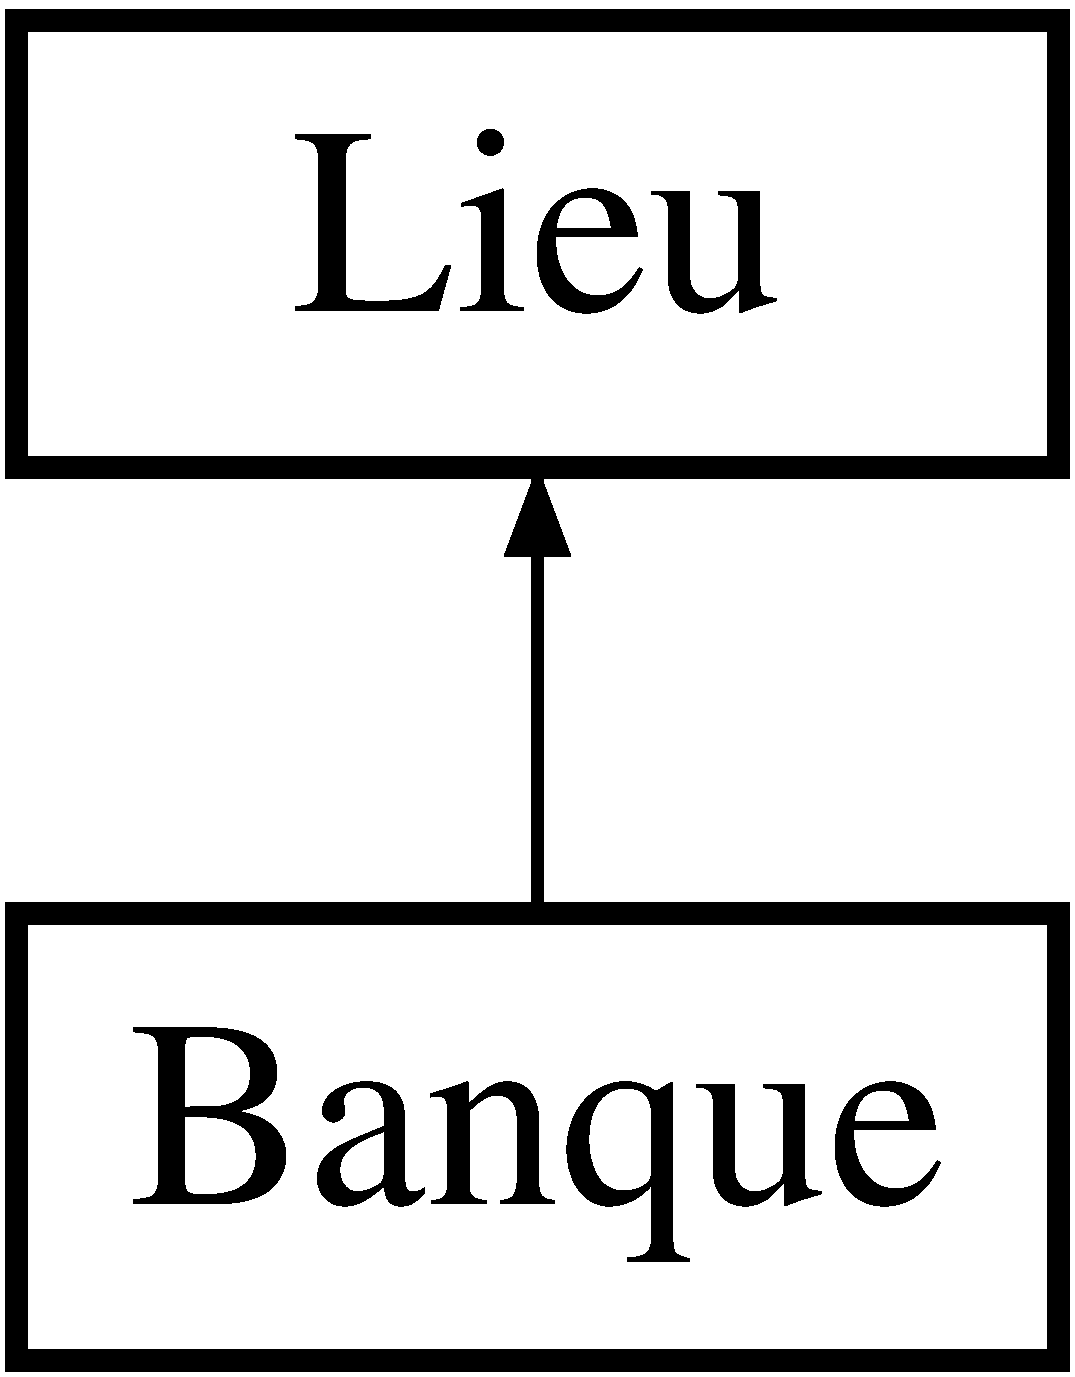
\includegraphics[height=2.000000cm]{class_banque}
\end{center}
\end{figure}
\subsection*{Public Member Functions}
\begin{DoxyCompactItemize}
\item 
\hyperlink{class_banque_aa15f21fa24ac647319aee3f8beb4b7f8}{Banque} ()
\begin{DoxyCompactList}\small\item\em Constructeur par défaut. \end{DoxyCompactList}\item 
\hyperlink{class_banque_ad861c8a9604be0acd1340ce108451b63}{Banque} (vector$<$ \hyperlink{class_objet}{Objet} $>$ \hyperlink{class_lieu_a3a65fbb8ecba3f2e265905730ad2e631}{objets\-Dispo}, int \hyperlink{class_lieu_a90b76b521f92a43626ccd29ed5a29f89}{cash\-Cache}, vector$<$ \hyperlink{class_p_n_j}{P\-N\-J} $>$ \hyperlink{class_lieu_a8c1e20b105f7972f22d8f16651de4ebd}{liste\-P\-N\-J}, string \hyperlink{class_lieu_a1e48889fe5c581f043b8bd77ca497fc7}{nom\-Lieu}, vector$<$ string $>$ action\-Vec)
\begin{DoxyCompactList}\small\item\em Constructeur de la classe \hyperlink{class_banque}{Banque}. \end{DoxyCompactList}\item 
virtual \hyperlink{class_banque_a14aaf09b3db8037f8d0007958fa7def2}{$\sim$\-Banque} ()
\begin{DoxyCompactList}\small\item\em Destructeur par défaut. \end{DoxyCompactList}\item 
void \hyperlink{class_banque_a24f76bd9177ebdef767e6bcbdc491535}{set\-Cash\-Banque} (int Cash\-Banque)
\begin{DoxyCompactList}\small\item\em stock la valeur de la variable Cash\-Banque dans la variable Cash\-Banque. \end{DoxyCompactList}\item 
void \hyperlink{class_banque_a8b9265c9c4d5df37631054f88ccb5f60}{deposer\-Cash} (\hyperlink{class_heros}{Heros} $\ast$heros, int cash)
\begin{DoxyCompactList}\small\item\em Incrémente le Cash\-Banque d'une valeur cash de la variable cash. \end{DoxyCompactList}\item 
int \hyperlink{class_banque_afe8de2a23d1e568be91811734a749197}{get\-Cash\-Banque} ()
\begin{DoxyCompactList}\small\item\em Accède à la variable Cash\-Banque. \end{DoxyCompactList}\item 
void \hyperlink{class_banque_a8729fd0d7255c82916fab90dd17c995a}{retirer\-Cash} (\hyperlink{class_heros}{Heros} $\ast$heros, int cash)
\begin{DoxyCompactList}\small\item\em Décrémente le Cash\-Banque d'une valeur cash de la variable cash. \end{DoxyCompactList}\item 
void \hyperlink{class_banque_ab6c629552a916ee9515a8c85bd5dc311}{executer\-Action} (\hyperlink{class_jeu}{Jeu} jeu, \hyperlink{class_heros}{Heros} $\ast$heros, \hyperlink{class_ville}{Ville} $\ast$ville)
\begin{DoxyCompactList}\small\item\em Exécute une action parmi les actions possibles par exemple Déposer, Retirer, Fouiller, Afficher Sac , Afficher stats du héros ou Quitter la banque. \end{DoxyCompactList}\end{DoxyCompactItemize}
\subsection*{Additional Inherited Members}


\subsection{Detailed Description}
Classe représentant la banque. 

\subsection{Constructor \& Destructor Documentation}
\hypertarget{class_banque_aa15f21fa24ac647319aee3f8beb4b7f8}{\index{Banque@{Banque}!Banque@{Banque}}
\index{Banque@{Banque}!Banque@{Banque}}
\subsubsection[{Banque}]{\setlength{\rightskip}{0pt plus 5cm}Banque\-::\-Banque (
\begin{DoxyParamCaption}
{}
\end{DoxyParamCaption}
)}}\label{class_banque_aa15f21fa24ac647319aee3f8beb4b7f8}


Constructeur par défaut. 


\begin{DoxyCode}
19 \{this->cashBanque = 0 ;\}
\end{DoxyCode}
\hypertarget{class_banque_ad861c8a9604be0acd1340ce108451b63}{\index{Banque@{Banque}!Banque@{Banque}}
\index{Banque@{Banque}!Banque@{Banque}}
\subsubsection[{Banque}]{\setlength{\rightskip}{0pt plus 5cm}Banque\-::\-Banque (
\begin{DoxyParamCaption}
\item[{vector$<$ {\bf Objet} $>$}]{objets\-Dispo, }
\item[{int}]{cash\-Cache, }
\item[{vector$<$ {\bf P\-N\-J} $>$}]{liste\-P\-N\-J, }
\item[{string}]{nom\-Lieu, }
\item[{vector$<$ string $>$}]{action\-Vec}
\end{DoxyParamCaption}
)}}\label{class_banque_ad861c8a9604be0acd1340ce108451b63}


Constructeur de la classe \hyperlink{class_banque}{Banque}. 


\begin{DoxyParams}{Parameters}
{\em objets\-Dispo} & Les objets disponibles à la banque. \\
\hline
{\em cashcache} & Le cash caché dans la banque. \\
\hline
{\em liste\-P\-N\-J} & Les \hyperlink{class_p_n_j}{P\-N\-J} présents dans la banque. \\
\hline
{\em nom\-Lieu} & Le nom de la banque. \\
\hline
{\em action\-Vec} & le vecteur des actions disponibles dans la banque. \\
\hline
\end{DoxyParams}

\begin{DoxyCode}
20                                                                                                            
                  :\hyperlink{class_lieu_a0b3086d598fc1bfc0b4c09ae96304b3a}{Lieu}(\hyperlink{class_lieu_a3a65fbb8ecba3f2e265905730ad2e631}{objetsDispo}, \hyperlink{class_lieu_a90b76b521f92a43626ccd29ed5a29f89}{cashCache}, \hyperlink{class_lieu_a8c1e20b105f7972f22d8f16651de4ebd}{listePNJ}, \textcolor{stringliteral}{"Banque"}, actionVec)\{
21     this->cashBanque = 0 ;\}
\end{DoxyCode}
\hypertarget{class_banque_a14aaf09b3db8037f8d0007958fa7def2}{\index{Banque@{Banque}!$\sim$\-Banque@{$\sim$\-Banque}}
\index{$\sim$\-Banque@{$\sim$\-Banque}!Banque@{Banque}}
\subsubsection[{$\sim$\-Banque}]{\setlength{\rightskip}{0pt plus 5cm}Banque\-::$\sim$\-Banque (
\begin{DoxyParamCaption}
{}
\end{DoxyParamCaption}
)\hspace{0.3cm}{\ttfamily [virtual]}}}\label{class_banque_a14aaf09b3db8037f8d0007958fa7def2}


Destructeur par défaut. 


\begin{DoxyCode}
62 \{\}
\end{DoxyCode}


\subsection{Member Function Documentation}
\hypertarget{class_banque_a8b9265c9c4d5df37631054f88ccb5f60}{\index{Banque@{Banque}!deposer\-Cash@{deposer\-Cash}}
\index{deposer\-Cash@{deposer\-Cash}!Banque@{Banque}}
\subsubsection[{deposer\-Cash}]{\setlength{\rightskip}{0pt plus 5cm}void Banque\-::deposer\-Cash (
\begin{DoxyParamCaption}
\item[{{\bf Heros} $\ast$}]{heros, }
\item[{int}]{cash}
\end{DoxyParamCaption}
)}}\label{class_banque_a8b9265c9c4d5df37631054f88ccb5f60}


Incrémente le Cash\-Banque d'une valeur cash de la variable cash. 


\begin{DoxyCode}
43                                                     \{
44         \textcolor{keywordflow}{if} (heros->\hyperlink{class_heros_a77bdee21cb8c8356448bb6669941441c}{getCash}() >= cash) \{
45             cashBanque+=cash;
46             heros->\hyperlink{class_heros_ae87dba7afa03e7fdacfc3a7e82d3a6a3}{setCash}(heros->\hyperlink{class_heros_a77bdee21cb8c8356448bb6669941441c}{getCash}() - cash);
47 
48         \}
49         \textcolor{keywordflow}{else} \{\}
50   \}
\end{DoxyCode}
\hypertarget{class_banque_ab6c629552a916ee9515a8c85bd5dc311}{\index{Banque@{Banque}!executer\-Action@{executer\-Action}}
\index{executer\-Action@{executer\-Action}!Banque@{Banque}}
\subsubsection[{executer\-Action}]{\setlength{\rightskip}{0pt plus 5cm}void Banque\-::executer\-Action (
\begin{DoxyParamCaption}
\item[{{\bf Jeu}}]{jeu, }
\item[{{\bf Heros} $\ast$}]{heros, }
\item[{{\bf Ville} $\ast$}]{ville}
\end{DoxyParamCaption}
)\hspace{0.3cm}{\ttfamily [virtual]}}}\label{class_banque_ab6c629552a916ee9515a8c85bd5dc311}


Exécute une action parmi les actions possibles par exemple Déposer, Retirer, Fouiller, Afficher Sac , Afficher stats du héros ou Quitter la banque. 


\begin{DoxyParams}{Parameters}
{\em jeu} & Une instance de la classe \hyperlink{class_jeu}{Jeu}. \\
\hline
{\em heros} & Une instance de la classe \hyperlink{class_heros}{Heros}. \\
\hline
\end{DoxyParams}


Reimplemented from \hyperlink{class_lieu_ad5d4e14283df04f0174f090f1614225c}{Lieu}.


\begin{DoxyCode}
64                                                                    \{
65 
66         \textcolor{keywordtype}{int} i=0, entree = -1 ;
67 
68     \textcolor{keywordflow}{while} (entree!=i+5) \{
69 
70         jeu.\hyperlink{class_jeu_aa09fb40439f16b9665a0d76679f78e4e}{afficherTexte}( \textcolor{stringliteral}{"Vous êtes dans le lieu suivant : "} + 
      \hyperlink{class_lieu_a1e48889fe5c581f043b8bd77ca497fc7}{nomLieu} + \textcolor{stringliteral}{". Que voulez-vous faire ? (entrée attendue : un numéro)"} );
71 
72 
73         \textcolor{keywordflow}{for} (i=0 ; i < \hyperlink{class_lieu_a8c1e20b105f7972f22d8f16651de4ebd}{listePNJ}.size(); i++) \{
74             jeu.\hyperlink{class_jeu_aa09fb40439f16b9665a0d76679f78e4e}{afficherTexte}(\hyperlink{banque_8cpp_a0d2f37137ee1fd6ff4a0ef803849dd63}{SSTR}(i) + \textcolor{stringliteral}{". Parler à la personne suivante :"} + 
      \hyperlink{class_lieu_a8c1e20b105f7972f22d8f16651de4ebd}{listePNJ}.at(i).getNom() );
75         \}
76 
77         jeu.\hyperlink{class_jeu_aa09fb40439f16b9665a0d76679f78e4e}{afficherTexte}(\hyperlink{banque_8cpp_a0d2f37137ee1fd6ff4a0ef803849dd63}{SSTR}(i) + \textcolor{stringliteral}{". "} + \textcolor{stringliteral}{"Déposer"} );
78 
79         jeu.\hyperlink{class_jeu_aa09fb40439f16b9665a0d76679f78e4e}{afficherTexte}(\hyperlink{banque_8cpp_a0d2f37137ee1fd6ff4a0ef803849dd63}{SSTR}(i+1) + \textcolor{stringliteral}{". "} + \textcolor{stringliteral}{"Retirer"} );
80 
81         jeu.\hyperlink{class_jeu_aa09fb40439f16b9665a0d76679f78e4e}{afficherTexte}(\hyperlink{banque_8cpp_a0d2f37137ee1fd6ff4a0ef803849dd63}{SSTR}(i+2) + \textcolor{stringliteral}{". "} + \textcolor{stringliteral}{"Fouiller"} );
82 
83         jeu.\hyperlink{class_jeu_aa09fb40439f16b9665a0d76679f78e4e}{afficherTexte}(\hyperlink{banque_8cpp_a0d2f37137ee1fd6ff4a0ef803849dd63}{SSTR}(i+3) + \textcolor{stringliteral}{". "} + \textcolor{stringliteral}{"Afficher Sac"} );
84 
85         jeu.\hyperlink{class_jeu_aa09fb40439f16b9665a0d76679f78e4e}{afficherTexte}(\hyperlink{banque_8cpp_a0d2f37137ee1fd6ff4a0ef803849dd63}{SSTR}(i+4) + \textcolor{stringliteral}{". "} + \textcolor{stringliteral}{"Afficher Stats du Héros"} );
86 
87         jeu.\hyperlink{class_jeu_aa09fb40439f16b9665a0d76679f78e4e}{afficherTexte}(\hyperlink{banque_8cpp_a0d2f37137ee1fd6ff4a0ef803849dd63}{SSTR}(i+5) + \textcolor{stringliteral}{". "} + \textcolor{stringliteral}{"Quitter"} );
88 
89 
90 
91         entree = jeu.\hyperlink{class_jeu_ac504a2a26ad7aa3c4281f8ab40cdc445}{demanderEntreeUtilisateur}(\textcolor{stringliteral}{"Faites votre choix :"});
92         \textcolor{keywordflow}{while} (entree < 0 or entree > i+5) \{
93             entree = jeu.\hyperlink{class_jeu_ac504a2a26ad7aa3c4281f8ab40cdc445}{demanderEntreeUtilisateur}(\textcolor{stringliteral}{"Faites un choix CORRECT :"});
94         \}
95 
96         \textcolor{keywordflow}{if} ( entree >= 0 and entree < i )
97             jeu.\hyperlink{class_jeu_aa09fb40439f16b9665a0d76679f78e4e}{afficherTexte}( heros->\hyperlink{class_heros_a4052af6e407ebdf4918e62340d374829}{ParleAPNJ}(&\hyperlink{class_lieu_a8c1e20b105f7972f22d8f16651de4ebd}{listePNJ}.at(entree), jeu) ) 
      ;
98 
99         \textcolor{keywordflow}{else} \textcolor{keywordflow}{if} ( entree == i )\{
100 
101             entree = -1 ;
102 
103             \textcolor{keywordflow}{while} ( entree < 0 or entree > heros->\hyperlink{class_heros_a77bdee21cb8c8356448bb6669941441c}{getCash}() ) \{
104                 entree = jeu.\hyperlink{class_jeu_ac504a2a26ad7aa3c4281f8ab40cdc445}{demanderEntreeUtilisateur}(\textcolor{stringliteral}{"Votre cash en portefeuille
       s'élève à : "} + \hyperlink{banque_8cpp_a0d2f37137ee1fd6ff4a0ef803849dd63}{SSTR}(heros->\hyperlink{class_heros_a77bdee21cb8c8356448bb6669941441c}{getCash}()) + \textcolor{stringliteral}{". Combien voulez-vous déposer ? Entrez 0 pour annuler"}
      );
105             \}
106 
107             \hyperlink{class_banque_a8b9265c9c4d5df37631054f88ccb5f60}{deposerCash}(heros, entree);
108             jeu.\hyperlink{class_jeu_aa09fb40439f16b9665a0d76679f78e4e}{afficherTexte}(\textcolor{stringliteral}{"Cash déposé: "} + \hyperlink{banque_8cpp_a0d2f37137ee1fd6ff4a0ef803849dd63}{SSTR}(entree) + \textcolor{stringliteral}{". Nouveau cash en banque: 
      "} + \hyperlink{banque_8cpp_a0d2f37137ee1fd6ff4a0ef803849dd63}{SSTR}(cashBanque) + \textcolor{stringliteral}{". Nouveau cash en portefeuille: "} + \hyperlink{banque_8cpp_a0d2f37137ee1fd6ff4a0ef803849dd63}{SSTR}(heros->
      \hyperlink{class_heros_a77bdee21cb8c8356448bb6669941441c}{getCash}()));
109 
110         \}
111 
112         \textcolor{keywordflow}{else} \textcolor{keywordflow}{if} ( entree == i+1 )\{
113 
114             entree = -1 ;
115 
116             \textcolor{keywordflow}{while} ( entree < 0 or entree > cashBanque ) \{
117                 entree = jeu.\hyperlink{class_jeu_ac504a2a26ad7aa3c4281f8ab40cdc445}{demanderEntreeUtilisateur}(\textcolor{stringliteral}{"Votre cash en banque
       s'élève à : "} + \hyperlink{banque_8cpp_a0d2f37137ee1fd6ff4a0ef803849dd63}{SSTR}(cashBanque) + \textcolor{stringliteral}{". Combien voulez-vous retirer ? Entrez 0 pour annuler"});
118             \}
119 
120             \hyperlink{class_banque_a8729fd0d7255c82916fab90dd17c995a}{retirerCash}(heros, entree);
121             jeu.\hyperlink{class_jeu_aa09fb40439f16b9665a0d76679f78e4e}{afficherTexte}(\textcolor{stringliteral}{"Cash retiré: "} + \hyperlink{banque_8cpp_a0d2f37137ee1fd6ff4a0ef803849dd63}{SSTR}(entree) + \textcolor{stringliteral}{". Nouveau cash en banque: 
      "} + \hyperlink{banque_8cpp_a0d2f37137ee1fd6ff4a0ef803849dd63}{SSTR}(cashBanque) + \textcolor{stringliteral}{". Nouveau cash en portefeuille: "} + \hyperlink{banque_8cpp_a0d2f37137ee1fd6ff4a0ef803849dd63}{SSTR}(heros->
      \hyperlink{class_heros_a77bdee21cb8c8356448bb6669941441c}{getCash}()));
122 
123 
124         \}
125 
126         \textcolor{keywordflow}{else} \textcolor{keywordflow}{if} ( entree == i+2 )\{
127 
128             \hyperlink{class_lieu_a90d7fd86c93e59830e20156ddb7aeb50}{fouiller}(jeu, heros);
129 
130         \}
131 
132         \textcolor{keywordflow}{else} \textcolor{keywordflow}{if} ( entree == i+3 )\{
133 
134             jeu.\hyperlink{class_jeu_a26c7a428a96b1f987150cb708fa7d903}{consommersac}(heros);
135 
136         \}
137 
138         \textcolor{keywordflow}{else} \textcolor{keywordflow}{if} ( entree == i+4 )\{
139 
140             jeu.\hyperlink{class_jeu_a7f9e3b8e6f3ad5d2c47ae29c54f2bdc4}{affichageStatsHero}(*heros);
141 
142         \}
143 
144         \textcolor{keywordflow}{else} \textcolor{keywordflow}{if} ( entree == i+5 )\{
145             jeu.\hyperlink{class_jeu_a52ce4fb6c415b45209db13a589c9d675}{timer}(4, \textcolor{stringliteral}{"retourn à la ville"});
146             heros->\hyperlink{class_heros_a8decc0b04f6724de10d2e2a8d1c3395c}{setLieuActuel}(ville);
147 
148         \}
149 
150         \textcolor{keywordflow}{else} \{\}
151 
152     \}
153     \}
\end{DoxyCode}
\hypertarget{class_banque_afe8de2a23d1e568be91811734a749197}{\index{Banque@{Banque}!get\-Cash\-Banque@{get\-Cash\-Banque}}
\index{get\-Cash\-Banque@{get\-Cash\-Banque}!Banque@{Banque}}
\subsubsection[{get\-Cash\-Banque}]{\setlength{\rightskip}{0pt plus 5cm}int Banque\-::get\-Cash\-Banque (
\begin{DoxyParamCaption}
{}
\end{DoxyParamCaption}
)}}\label{class_banque_afe8de2a23d1e568be91811734a749197}


Accède à la variable Cash\-Banque. 

\begin{DoxyReturn}{Returns}
La valeur de la variable Cash\-Banque. 
\end{DoxyReturn}

\begin{DoxyCode}
38                                  \{
39         \textcolor{keywordflow}{return} cashBanque;
40   \}
\end{DoxyCode}
\hypertarget{class_banque_a8729fd0d7255c82916fab90dd17c995a}{\index{Banque@{Banque}!retirer\-Cash@{retirer\-Cash}}
\index{retirer\-Cash@{retirer\-Cash}!Banque@{Banque}}
\subsubsection[{retirer\-Cash}]{\setlength{\rightskip}{0pt plus 5cm}void Banque\-::retirer\-Cash (
\begin{DoxyParamCaption}
\item[{{\bf Heros} $\ast$}]{heros, }
\item[{int}]{cash}
\end{DoxyParamCaption}
)}}\label{class_banque_a8729fd0d7255c82916fab90dd17c995a}


Décrémente le Cash\-Banque d'une valeur cash de la variable cash. 


\begin{DoxyCode}
52                                                   \{
53         \textcolor{keywordflow}{if} (cashBanque >= cash) \{
54             cashBanque-=cash;
55             heros->\hyperlink{class_heros_ae87dba7afa03e7fdacfc3a7e82d3a6a3}{setCash}(heros->\hyperlink{class_heros_a77bdee21cb8c8356448bb6669941441c}{getCash}() + cash);
56 
57         \}
58         \textcolor{keywordflow}{else} \{\}
59 
60     \}
\end{DoxyCode}
\hypertarget{class_banque_a24f76bd9177ebdef767e6bcbdc491535}{\index{Banque@{Banque}!set\-Cash\-Banque@{set\-Cash\-Banque}}
\index{set\-Cash\-Banque@{set\-Cash\-Banque}!Banque@{Banque}}
\subsubsection[{set\-Cash\-Banque}]{\setlength{\rightskip}{0pt plus 5cm}void Banque\-::set\-Cash\-Banque (
\begin{DoxyParamCaption}
\item[{int}]{Cash\-Banque}
\end{DoxyParamCaption}
)}}\label{class_banque_a24f76bd9177ebdef767e6bcbdc491535}


stock la valeur de la variable Cash\-Banque dans la variable Cash\-Banque. 


\begin{DoxyCode}
34                                                 \{
35             cashBanque = CashBanque;
36   \}
\end{DoxyCode}


The documentation for this class was generated from the following files\-:\begin{DoxyCompactItemize}
\item 
/nfs/usersgm/\-G\-M26/neljibbawe/\-Bureau/\-Projet\-C\-P\-P\-A\-Rendre/\-C\-P\-P R\-P\-G/\-R\-P\-G/\hyperlink{banque_8hpp}{banque.\-hpp}\item 
/nfs/usersgm/\-G\-M26/neljibbawe/\-Bureau/\-Projet\-C\-P\-P\-A\-Rendre/\-C\-P\-P R\-P\-G/\-R\-P\-G/\hyperlink{banque_8cpp}{banque.\-cpp}\end{DoxyCompactItemize}

\hypertarget{class_consommable}{\section{Consommable Class Reference}
\label{class_consommable}\index{Consommable@{Consommable}}
}


Classe représentant les objets consommables.  




{\ttfamily \#include $<$consommable.\-hpp$>$}

Inheritance diagram for Consommable\-:\begin{figure}[H]
\begin{center}
\leavevmode
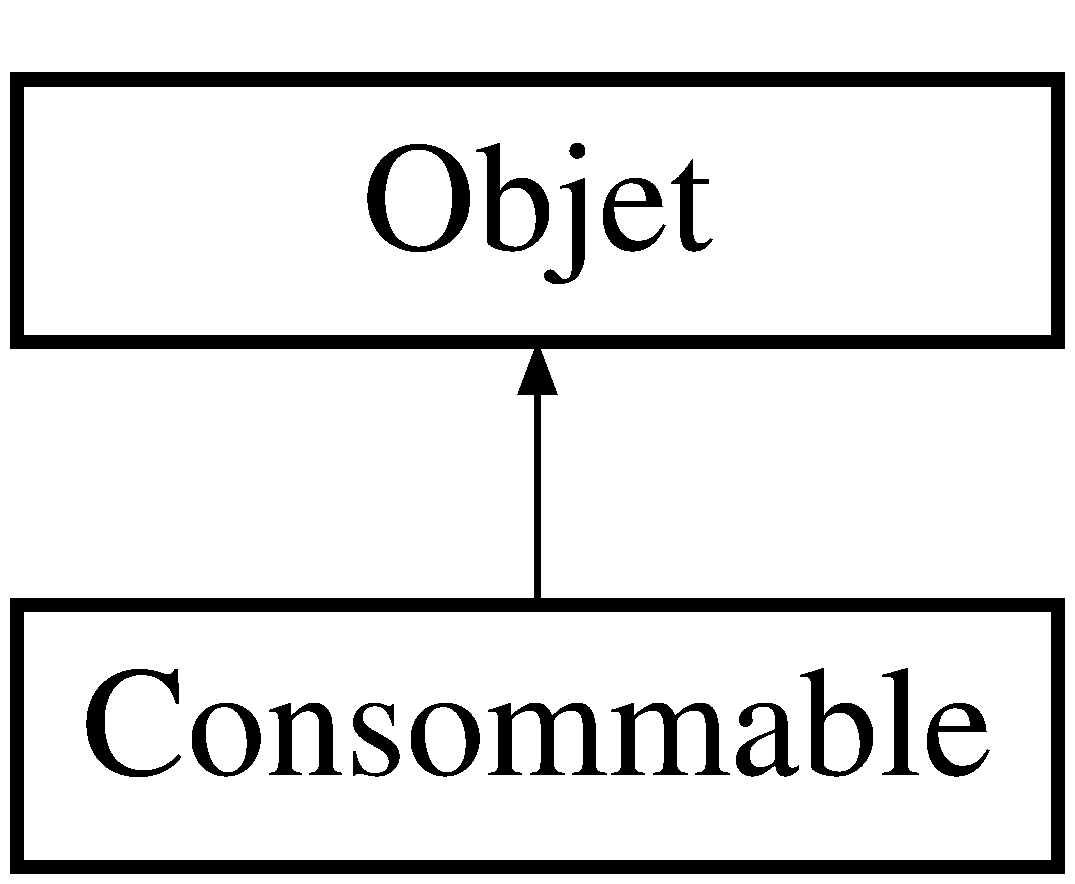
\includegraphics[height=2.000000cm]{class_consommable}
\end{center}
\end{figure}
\subsection*{Public Member Functions}
\begin{DoxyCompactItemize}
\item 
\hyperlink{class_consommable_a690f64c7cd8eaa64f4db98f170706864}{Consommable} (int acc\-Objet, int p, string nom\-Obj, int vf, int qte\-Obj, int valeur\-Energie, int valeur\-Intel)
\begin{DoxyCompactList}\small\item\em Constructeur de la classe \hyperlink{class_consommable}{Consommable}. \end{DoxyCompactList}\item 
\hyperlink{class_consommable_ad87f63d0fef7c1424270bdf334857d4d}{Consommable} ()
\begin{DoxyCompactList}\small\item\em Constructeur par défaut. \end{DoxyCompactList}\item 
void \hyperlink{class_consommable_a23a0a6e80f5cb5ff1269514389d70413}{set\-Valeur\-Intel} (int valeur\-Intel)
\begin{DoxyCompactList}\small\item\em stock la valeur de la variable valeur\-Intel dans la variable valeur\-Intel. \end{DoxyCompactList}\item 
int \hyperlink{class_consommable_aafb68bb944bfc5c3fee60d8d3ffba241}{get\-Valeur\-Intel} ()
\begin{DoxyCompactList}\small\item\em Accède à la variable valeur\-Intel. \end{DoxyCompactList}\item 
void \hyperlink{class_consommable_ac70bcac8ceed2be2a4b09a36874bc752}{set\-Valeur\-Energie} (int var)
\begin{DoxyCompactList}\small\item\em stock la valeur de la variable var dans la variable valeur\-Intel. \end{DoxyCompactList}\item 
int \hyperlink{class_consommable_a14eacc0565fc9afb5b2f2b510f8daff7}{get\-Valeur\-Energie} ()
\begin{DoxyCompactList}\small\item\em Accède à la variable valeur\-Energie. \end{DoxyCompactList}\item 
void \hyperlink{class_consommable_ab2105902385a78cbca8496fdde262d2f}{utiliser\-Objet} (\hyperlink{class_jeu}{Jeu} jeu, \hyperlink{class_heros}{Heros} $\ast$heros)
\begin{DoxyCompactList}\small\item\em En consommant l'objet, permet à l'héros de gagner de l'énergie, de la force et de l'intelligence. \end{DoxyCompactList}\end{DoxyCompactItemize}
\subsection*{Additional Inherited Members}


\subsection{Detailed Description}
Classe représentant les objets consommables. 

\subsection{Constructor \& Destructor Documentation}
\hypertarget{class_consommable_a690f64c7cd8eaa64f4db98f170706864}{\index{Consommable@{Consommable}!Consommable@{Consommable}}
\index{Consommable@{Consommable}!Consommable@{Consommable}}
\subsubsection[{Consommable}]{\setlength{\rightskip}{0pt plus 5cm}Consommable\-::\-Consommable (
\begin{DoxyParamCaption}
\item[{int}]{acc\-Objet, }
\item[{int}]{p, }
\item[{string}]{nom\-Obj, }
\item[{int}]{vf, }
\item[{int}]{qte\-Obj, }
\item[{int}]{valeur\-Energie, }
\item[{int}]{valeur\-Intel}
\end{DoxyParamCaption}
)}}\label{class_consommable_a690f64c7cd8eaa64f4db98f170706864}


Constructeur de la classe \hyperlink{class_consommable}{Consommable}. 


\begin{DoxyParams}{Parameters}
{\em acc\-Objet} & L'accessibilité de l'objet à partir d'un certain âge. \\
\hline
{\em p} & Le prix de l'objet. \\
\hline
{\em nom\-Obj} & Le nom de l'objet. \\
\hline
{\em vf} & La valeur force que l'héros gagne en consommant l'objet. \\
\hline
{\em qte\-Obj} & La quantité de l'objet. \\
\hline
{\em valeur\-Energie} & La valeur d'énergie que l'héros gagne en consommant l'objet. \\
\hline
{\em valeur\-Intel} & La valeur d'intelligence que l'héros gagne en consomment l'objet. \\
\hline
\end{DoxyParams}

\begin{DoxyCode}
13                                                                                                            
         : \hyperlink{class_objet_aefdd826d50085897e4894ffef4597d04}{Objet}(accObjet, p, nomObj, vf, qteObj) \{
14     valeurIntel = valIntel;
15     valeurEnergie = valEnergie;
16     \}
\end{DoxyCode}
\hypertarget{class_consommable_ad87f63d0fef7c1424270bdf334857d4d}{\index{Consommable@{Consommable}!Consommable@{Consommable}}
\index{Consommable@{Consommable}!Consommable@{Consommable}}
\subsubsection[{Consommable}]{\setlength{\rightskip}{0pt plus 5cm}Consommable\-::\-Consommable (
\begin{DoxyParamCaption}
{}
\end{DoxyParamCaption}
)}}\label{class_consommable_ad87f63d0fef7c1424270bdf334857d4d}


Constructeur par défaut. 


\begin{DoxyCode}
12 \{\}
\end{DoxyCode}


\subsection{Member Function Documentation}
\hypertarget{class_consommable_a14eacc0565fc9afb5b2f2b510f8daff7}{\index{Consommable@{Consommable}!get\-Valeur\-Energie@{get\-Valeur\-Energie}}
\index{get\-Valeur\-Energie@{get\-Valeur\-Energie}!Consommable@{Consommable}}
\subsubsection[{get\-Valeur\-Energie}]{\setlength{\rightskip}{0pt plus 5cm}int Consommable\-::get\-Valeur\-Energie (
\begin{DoxyParamCaption}
{}
\end{DoxyParamCaption}
)}}\label{class_consommable_a14eacc0565fc9afb5b2f2b510f8daff7}


Accède à la variable valeur\-Energie. 

\begin{DoxyReturn}{Returns}
La valeur de la variable valeur\-Energie. 
\end{DoxyReturn}

\begin{DoxyCode}
29                                    \{
30     \textcolor{keywordflow}{return} valeurEnergie;
31   \}
\end{DoxyCode}
\hypertarget{class_consommable_aafb68bb944bfc5c3fee60d8d3ffba241}{\index{Consommable@{Consommable}!get\-Valeur\-Intel@{get\-Valeur\-Intel}}
\index{get\-Valeur\-Intel@{get\-Valeur\-Intel}!Consommable@{Consommable}}
\subsubsection[{get\-Valeur\-Intel}]{\setlength{\rightskip}{0pt plus 5cm}int Consommable\-::get\-Valeur\-Intel (
\begin{DoxyParamCaption}
{}
\end{DoxyParamCaption}
)}}\label{class_consommable_aafb68bb944bfc5c3fee60d8d3ffba241}


Accède à la variable valeur\-Intel. 

\begin{DoxyReturn}{Returns}
La valeur de la variable valeur\-Intel. 
\end{DoxyReturn}

\begin{DoxyCode}
22                                        \{
23     \textcolor{keywordflow}{return} valeurIntel;
24   \}
\end{DoxyCode}
\hypertarget{class_consommable_ac70bcac8ceed2be2a4b09a36874bc752}{\index{Consommable@{Consommable}!set\-Valeur\-Energie@{set\-Valeur\-Energie}}
\index{set\-Valeur\-Energie@{set\-Valeur\-Energie}!Consommable@{Consommable}}
\subsubsection[{set\-Valeur\-Energie}]{\setlength{\rightskip}{0pt plus 5cm}void Consommable\-::set\-Valeur\-Energie (
\begin{DoxyParamCaption}
\item[{int}]{var}
\end{DoxyParamCaption}
)}}\label{class_consommable_ac70bcac8ceed2be2a4b09a36874bc752}


stock la valeur de la variable var dans la variable valeur\-Intel. 


\begin{DoxyCode}
26                                             \{
27     valeurEnergie=var;
28   \}
\end{DoxyCode}
\hypertarget{class_consommable_a23a0a6e80f5cb5ff1269514389d70413}{\index{Consommable@{Consommable}!set\-Valeur\-Intel@{set\-Valeur\-Intel}}
\index{set\-Valeur\-Intel@{set\-Valeur\-Intel}!Consommable@{Consommable}}
\subsubsection[{set\-Valeur\-Intel}]{\setlength{\rightskip}{0pt plus 5cm}void Consommable\-::set\-Valeur\-Intel (
\begin{DoxyParamCaption}
\item[{int}]{valeur\-Intel}
\end{DoxyParamCaption}
)}}\label{class_consommable_a23a0a6e80f5cb5ff1269514389d70413}


stock la valeur de la variable valeur\-Intel dans la variable valeur\-Intel. 


\begin{DoxyCode}
18                                                       \{
19       this->valeurIntel = valeurIntel;
20   \}
\end{DoxyCode}
\hypertarget{class_consommable_ab2105902385a78cbca8496fdde262d2f}{\index{Consommable@{Consommable}!utiliser\-Objet@{utiliser\-Objet}}
\index{utiliser\-Objet@{utiliser\-Objet}!Consommable@{Consommable}}
\subsubsection[{utiliser\-Objet}]{\setlength{\rightskip}{0pt plus 5cm}void Consommable\-::utiliser\-Objet (
\begin{DoxyParamCaption}
\item[{{\bf Jeu}}]{jeu, }
\item[{{\bf Heros} $\ast$}]{heros}
\end{DoxyParamCaption}
)\hspace{0.3cm}{\ttfamily [virtual]}}}\label{class_consommable_ab2105902385a78cbca8496fdde262d2f}


En consommant l'objet, permet à l'héros de gagner de l'énergie, de la force et de l'intelligence. 


\begin{DoxyParams}{Parameters}
{\em jeu} & Une instance de la classe \hyperlink{class_jeu}{Jeu}. \\
\hline
{\em heros} & Un pointeur sur la classe Héros. \\
\hline
\end{DoxyParams}


Reimplemented from \hyperlink{class_objet_ab8c32a2e0b236fcf75a06a2edc1f71b6}{Objet}.


\begin{DoxyCode}
32                                                       \{
33       heros->\hyperlink{class_heros_a5d4f5d3d3a4db451923f0609a3e1b53c}{setEnergie}(heros->\hyperlink{class_heros_ae9bbef6d2edcb8b14d9ec3854146a42c}{getEnergie}()+ valeurEnergie);
34       heros->\hyperlink{class_personnage_af8b3c4f6c0f7035678d9ecf574976650}{setIntelligence}(heros->\hyperlink{class_personnage_a250eec1aba0df7a105dd564e4cd02b0b}{getIntelligence}() + valeurIntel);
35       heros->\hyperlink{class_personnage_a6745d147720906f2c85ddce11981d71f}{setForce}(heros->\hyperlink{class_personnage_a40de0ba95f25eb6f1653b6a4183763ae}{getForce}() + \hyperlink{class_objet_aa819b02977c333c0cc5e116575e951cc}{valeurForce});
36       jeu.\hyperlink{class_jeu_aa09fb40439f16b9665a0d76679f78e4e}{afficherTexte}(\textcolor{stringliteral}{"Vous avez gagné "} + \hyperlink{consommable_8cpp_a0d2f37137ee1fd6ff4a0ef803849dd63}{SSTR}(valeurEnergie) + \textcolor{stringliteral}{" En energie et "} + 
      \hyperlink{consommable_8cpp_a0d2f37137ee1fd6ff4a0ef803849dd63}{SSTR}(valeurIntel)  + \textcolor{stringliteral}{" En Intelligence"});
37   \}
\end{DoxyCode}


The documentation for this class was generated from the following files\-:\begin{DoxyCompactItemize}
\item 
/nfs/usersgm/\-G\-M26/neljibbawe/\-Bureau/\-Projet\-C\-P\-P\-A\-Rendre/\-C\-P\-P R\-P\-G/\-R\-P\-G/\hyperlink{consommable_8hpp}{consommable.\-hpp}\item 
/nfs/usersgm/\-G\-M26/neljibbawe/\-Bureau/\-Projet\-C\-P\-P\-A\-Rendre/\-C\-P\-P R\-P\-G/\-R\-P\-G/\hyperlink{consommable_8cpp}{consommable.\-cpp}\end{DoxyCompactItemize}

\hypertarget{class_ecole}{\section{Ecole Class Reference}
\label{class_ecole}\index{Ecole@{Ecole}}
}


Classe représentant l'école.  




{\ttfamily \#include $<$ecole.\-hpp$>$}

Inheritance diagram for Ecole\-:\begin{figure}[H]
\begin{center}
\leavevmode
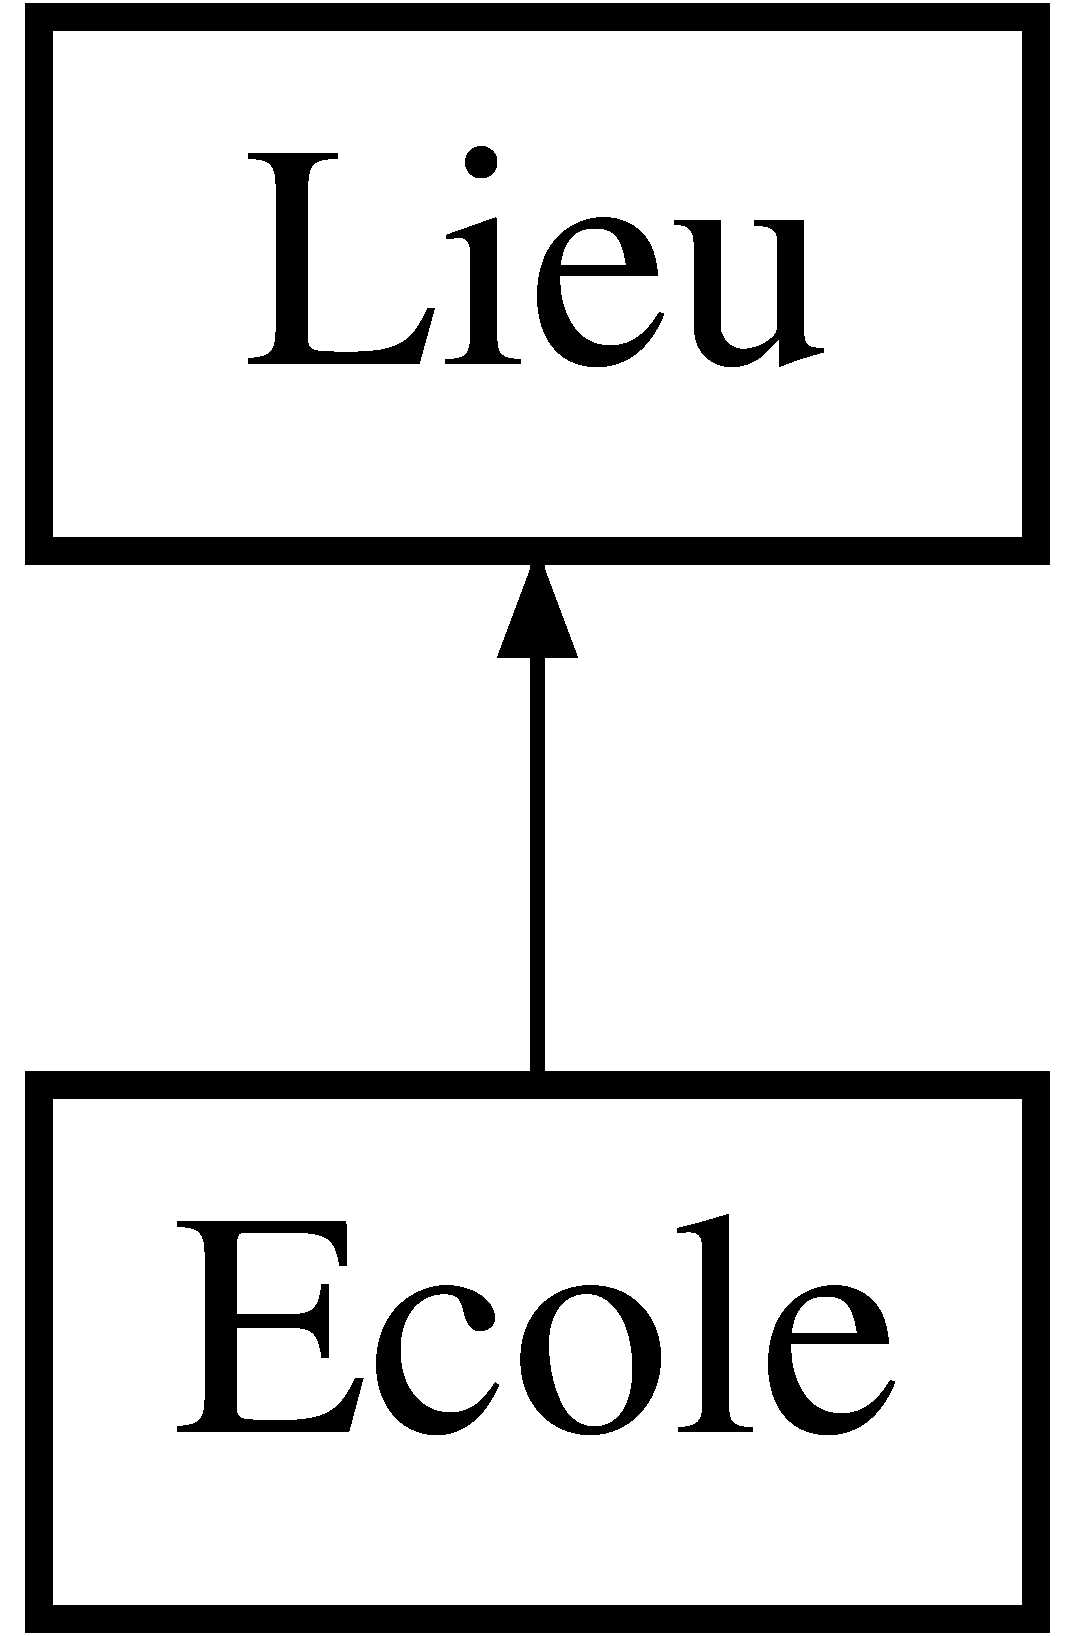
\includegraphics[height=2.000000cm]{class_ecole}
\end{center}
\end{figure}
\subsection*{Public Member Functions}
\begin{DoxyCompactItemize}
\item 
\hyperlink{class_ecole_a7bab5ff4118af8c59da282b62151653e}{Ecole} ()
\begin{DoxyCompactList}\small\item\em Constructeur par défaut. \end{DoxyCompactList}\item 
\hyperlink{class_ecole_a1630c88a0ebf2ce9e0e5220d1baaa34a}{Ecole} (vector$<$ \hyperlink{class_objet}{Objet} $>$ \hyperlink{class_lieu_a3a65fbb8ecba3f2e265905730ad2e631}{objets\-Dispo}, int \hyperlink{class_lieu_a90b76b521f92a43626ccd29ed5a29f89}{cash\-Cache}, vector$<$ \hyperlink{class_p_n_j}{P\-N\-J} $>$ \hyperlink{class_lieu_a8c1e20b105f7972f22d8f16651de4ebd}{liste\-P\-N\-J}, string \hyperlink{class_lieu_a1e48889fe5c581f043b8bd77ca497fc7}{nom\-Lieu}, vector$<$ string $>$ action\-Vec)
\begin{DoxyCompactList}\small\item\em Constructeur de la classe \hyperlink{class_ecole}{Ecole}. \end{DoxyCompactList}\item 
void \hyperlink{class_ecole_a717229b0b7a96d0093aa8b72db752ccd}{executer\-Action} (\hyperlink{class_jeu}{Jeu} jeu, \hyperlink{class_heros}{Heros} $\ast$heros, \hyperlink{class_ville}{Ville} $\ast$ville)
\begin{DoxyCompactList}\small\item\em Exécute une action parmi les actions possibles dans le lieu ecole comme parler à un \hyperlink{class_p_n_j}{P\-N\-J}, Faire du sport, Fouiller, Afficher sac ou Afficher stats du héros. \end{DoxyCompactList}\end{DoxyCompactItemize}
\subsection*{Additional Inherited Members}


\subsection{Detailed Description}
Classe représentant l'école. 

\subsection{Constructor \& Destructor Documentation}
\hypertarget{class_ecole_a7bab5ff4118af8c59da282b62151653e}{\index{Ecole@{Ecole}!Ecole@{Ecole}}
\index{Ecole@{Ecole}!Ecole@{Ecole}}
\subsubsection[{Ecole}]{\setlength{\rightskip}{0pt plus 5cm}Ecole\-::\-Ecole (
\begin{DoxyParamCaption}
{}
\end{DoxyParamCaption}
)}}\label{class_ecole_a7bab5ff4118af8c59da282b62151653e}


Constructeur par défaut. 


\begin{DoxyCode}
19 \{\}
\end{DoxyCode}
\hypertarget{class_ecole_a1630c88a0ebf2ce9e0e5220d1baaa34a}{\index{Ecole@{Ecole}!Ecole@{Ecole}}
\index{Ecole@{Ecole}!Ecole@{Ecole}}
\subsubsection[{Ecole}]{\setlength{\rightskip}{0pt plus 5cm}Ecole\-::\-Ecole (
\begin{DoxyParamCaption}
\item[{vector$<$ {\bf Objet} $>$}]{objets\-Dispo, }
\item[{int}]{cash\-Cache, }
\item[{vector$<$ {\bf P\-N\-J} $>$}]{liste\-P\-N\-J, }
\item[{string}]{nom\-Lieu, }
\item[{vector$<$ string $>$}]{action\-Vec}
\end{DoxyParamCaption}
)}}\label{class_ecole_a1630c88a0ebf2ce9e0e5220d1baaa34a}


Constructeur de la classe \hyperlink{class_ecole}{Ecole}. 


\begin{DoxyParams}{Parameters}
{\em objets\-Dispo} & Le vecteur des objets disponibles à l'école. \\
\hline
{\em cash\-Cache} & Le cash caché à l'école. \\
\hline
{\em liste\-P\-N\-J} & La liste des \hyperlink{class_p_n_j}{P\-N\-J} présents à l'école. \\
\hline
{\em nom\-Lieu} & c'est le nom du lieu ou se trouve l'héros ici c'est l'école. \\
\hline
{\em action\-Vec} & Le vecteur d'actons possibles à l'école. \\
\hline
\end{DoxyParams}

\begin{DoxyCode}
20                                                                                                            
                   : \hyperlink{class_lieu_a0b3086d598fc1bfc0b4c09ae96304b3a}{Lieu} (\hyperlink{class_lieu_a3a65fbb8ecba3f2e265905730ad2e631}{objetsDispo}, \hyperlink{class_lieu_a90b76b521f92a43626ccd29ed5a29f89}{cashCache}, \hyperlink{class_lieu_a8c1e20b105f7972f22d8f16651de4ebd}{listePNJ}, \textcolor{stringliteral}{"Ecole"}, actionVec)\{
21     \}
\end{DoxyCode}


\subsection{Member Function Documentation}
\hypertarget{class_ecole_a717229b0b7a96d0093aa8b72db752ccd}{\index{Ecole@{Ecole}!executer\-Action@{executer\-Action}}
\index{executer\-Action@{executer\-Action}!Ecole@{Ecole}}
\subsubsection[{executer\-Action}]{\setlength{\rightskip}{0pt plus 5cm}void Ecole\-::executer\-Action (
\begin{DoxyParamCaption}
\item[{{\bf Jeu}}]{jeu, }
\item[{{\bf Heros} $\ast$}]{heros, }
\item[{{\bf Ville} $\ast$}]{ville}
\end{DoxyParamCaption}
)\hspace{0.3cm}{\ttfamily [virtual]}}}\label{class_ecole_a717229b0b7a96d0093aa8b72db752ccd}


Exécute une action parmi les actions possibles dans le lieu ecole comme parler à un \hyperlink{class_p_n_j}{P\-N\-J}, Faire du sport, Fouiller, Afficher sac ou Afficher stats du héros. 


\begin{DoxyParams}{Parameters}
{\em jeu} & Une instance de la classe \hyperlink{class_jeu}{Jeu}. \\
\hline
{\em heros} & Un pointeur sur la classe Héros. \\
\hline
{\em ville} & Un pointeur sur la classe \hyperlink{class_ville}{Ville}. \\
\hline
\end{DoxyParams}


Reimplemented from \hyperlink{class_lieu_ad5d4e14283df04f0174f090f1614225c}{Lieu}.


\begin{DoxyCode}
35                                                               \{
36 
37         \textcolor{keywordtype}{int} i=0, entree = -1 ;
38     \textcolor{keywordflow}{while} (entree!=i+4) \{
39 
40         jeu.\hyperlink{class_jeu_aa09fb40439f16b9665a0d76679f78e4e}{afficherTexte}( \textcolor{stringliteral}{"Vous êtes dans le lieu suivant : Ecole. Que voulez-vous faire ?
       (entrée attendue : un numéro)"} );
41 
42 
43         \textcolor{keywordflow}{for} (i=0 ; i < \hyperlink{class_lieu_a8c1e20b105f7972f22d8f16651de4ebd}{listePNJ}.size(); i++) \{
44 
45         jeu.\hyperlink{class_jeu_aa09fb40439f16b9665a0d76679f78e4e}{afficherTexte}(\hyperlink{ecole_8cpp_a0d2f37137ee1fd6ff4a0ef803849dd63}{SSTR}(i) + \textcolor{stringliteral}{". Parler à la personne suivante :"} + 
      \hyperlink{class_lieu_a8c1e20b105f7972f22d8f16651de4ebd}{listePNJ}.at(i).getNom() );
46         \}
47         jeu.\hyperlink{class_jeu_aa09fb40439f16b9665a0d76679f78e4e}{afficherTexte}(\hyperlink{ecole_8cpp_a0d2f37137ee1fd6ff4a0ef803849dd63}{SSTR}(i) + \textcolor{stringliteral}{". Faire du sport"} );
48 
49         jeu.\hyperlink{class_jeu_aa09fb40439f16b9665a0d76679f78e4e}{afficherTexte}(\hyperlink{ecole_8cpp_a0d2f37137ee1fd6ff4a0ef803849dd63}{SSTR}(i+1) + \textcolor{stringliteral}{". "} + \textcolor{stringliteral}{"Fouiller"} );
50 
51         jeu.\hyperlink{class_jeu_aa09fb40439f16b9665a0d76679f78e4e}{afficherTexte}(\hyperlink{ecole_8cpp_a0d2f37137ee1fd6ff4a0ef803849dd63}{SSTR}(i+2) + \textcolor{stringliteral}{". "} + \textcolor{stringliteral}{"Afficher Sac"} );
52 
53         jeu.\hyperlink{class_jeu_aa09fb40439f16b9665a0d76679f78e4e}{afficherTexte}(\hyperlink{ecole_8cpp_a0d2f37137ee1fd6ff4a0ef803849dd63}{SSTR}(i+3) + \textcolor{stringliteral}{". "} + \textcolor{stringliteral}{"Afficher Stats du Héros"} );
54 
55         jeu.\hyperlink{class_jeu_aa09fb40439f16b9665a0d76679f78e4e}{afficherTexte}(\hyperlink{ecole_8cpp_a0d2f37137ee1fd6ff4a0ef803849dd63}{SSTR}(i+4) + \textcolor{stringliteral}{". "} + \textcolor{stringliteral}{"Quitter"} );
56 
57 
58 
59         entree = jeu.\hyperlink{class_jeu_ac504a2a26ad7aa3c4281f8ab40cdc445}{demanderEntreeUtilisateur}(\textcolor{stringliteral}{"Faites votre choix :"});
60         \textcolor{keywordflow}{while} (entree < 0 or entree > i+4) \{
61             entree = jeu.\hyperlink{class_jeu_ac504a2a26ad7aa3c4281f8ab40cdc445}{demanderEntreeUtilisateur}(\textcolor{stringliteral}{"Faites un choix CORRECT :"});
62         \}
63 
64         \textcolor{keywordflow}{if} ( entree >= 0 and entree < i )
65             jeu.\hyperlink{class_jeu_aa09fb40439f16b9665a0d76679f78e4e}{afficherTexte}( heros->\hyperlink{class_heros_a4052af6e407ebdf4918e62340d374829}{ParleAPNJ}(&\hyperlink{class_lieu_a8c1e20b105f7972f22d8f16651de4ebd}{listePNJ}.at(entree), jeu) ) 
      ;
66 
67         \textcolor{keywordflow}{else} \textcolor{keywordflow}{if} (entree == i) \{
68             \textcolor{keywordflow}{if} (heros->\hyperlink{class_heros_ae9bbef6d2edcb8b14d9ec3854146a42c}{getEnergie}()>heros->\hyperlink{class_heros_ae9bbef6d2edcb8b14d9ec3854146a42c}{getEnergie}()-4) \{
69             jeu.\hyperlink{class_jeu_a52ce4fb6c415b45209db13a589c9d675}{timer}(40/heros->\hyperlink{class_personnage_a40de0ba95f25eb6f1653b6a4183763ae}{getForce}(),\textcolor{stringliteral}{"Vous vous défoulez comme un fou !"});
70             heros->\hyperlink{class_personnage_a6745d147720906f2c85ddce11981d71f}{setForce}(heros->\hyperlink{class_personnage_a40de0ba95f25eb6f1653b6a4183763ae}{getForce}()+1);
71             heros->\hyperlink{class_heros_a5d4f5d3d3a4db451923f0609a3e1b53c}{setEnergie}(heros->\hyperlink{class_heros_ae9bbef6d2edcb8b14d9ec3854146a42c}{getEnergie}()-4);
72             jeu.\hyperlink{class_jeu_a52ce4fb6c415b45209db13a589c9d675}{timer}(1,\textcolor{stringliteral}{"Vous êtes épuisés ! Vous avez gagné 2 de force mais perdu 5 en énergie."});
73 
74             \}
75             \textcolor{keywordflow}{else} jeu.\hyperlink{class_jeu_aa09fb40439f16b9665a0d76679f78e4e}{afficherTexte}(\textcolor{stringliteral}{"Vous n'avez pas assez d'énergie... Allez vous reposer"});
76         \}
77         \textcolor{keywordflow}{else} \textcolor{keywordflow}{if} ( entree == i+1 )\{
78 
79             \hyperlink{class_lieu_a90d7fd86c93e59830e20156ddb7aeb50}{fouiller}(jeu, heros);
80 
81         \}
82 
83         \textcolor{keywordflow}{else} \textcolor{keywordflow}{if} ( entree == i+2 )\{
84 
85             jeu.\hyperlink{class_jeu_a26c7a428a96b1f987150cb708fa7d903}{consommersac}(heros);
86 
87         \}
88 
89         \textcolor{keywordflow}{else} \textcolor{keywordflow}{if} ( entree == i+3 )\{
90 
91             jeu.\hyperlink{class_jeu_a7f9e3b8e6f3ad5d2c47ae29c54f2bdc4}{affichageStatsHero}(*heros);
92 
93         \}
94 
95         \textcolor{keywordflow}{else} \textcolor{keywordflow}{if} ( entree == i+4 )\{
96             jeu.\hyperlink{class_jeu_a52ce4fb6c415b45209db13a589c9d675}{timer}(4, \textcolor{stringliteral}{"retour à la ville"});
97             heros->\hyperlink{class_heros_a8decc0b04f6724de10d2e2a8d1c3395c}{setLieuActuel}(ville);
98 
99         \}
100 
101         \textcolor{keywordflow}{else} \{\}
102 
103 
104     \}
105 
106 
107     \}
\end{DoxyCode}


The documentation for this class was generated from the following files\-:\begin{DoxyCompactItemize}
\item 
/nfs/usersgm/\-G\-M26/neljibbawe/\-Bureau/\-Projet\-C\-P\-P\-A\-Rendre/\-C\-P\-P R\-P\-G/\-R\-P\-G/\hyperlink{ecole_8hpp}{ecole.\-hpp}\item 
/nfs/usersgm/\-G\-M26/neljibbawe/\-Bureau/\-Projet\-C\-P\-P\-A\-Rendre/\-C\-P\-P R\-P\-G/\-R\-P\-G/\hyperlink{ecole_8cpp}{ecole.\-cpp}\end{DoxyCompactItemize}

\hypertarget{class_foret}{\section{Foret Class Reference}
\label{class_foret}\index{Foret@{Foret}}
}


Classe représentant la foret.  




{\ttfamily \#include $<$foret.\-hpp$>$}

Inheritance diagram for Foret\-:\begin{figure}[H]
\begin{center}
\leavevmode
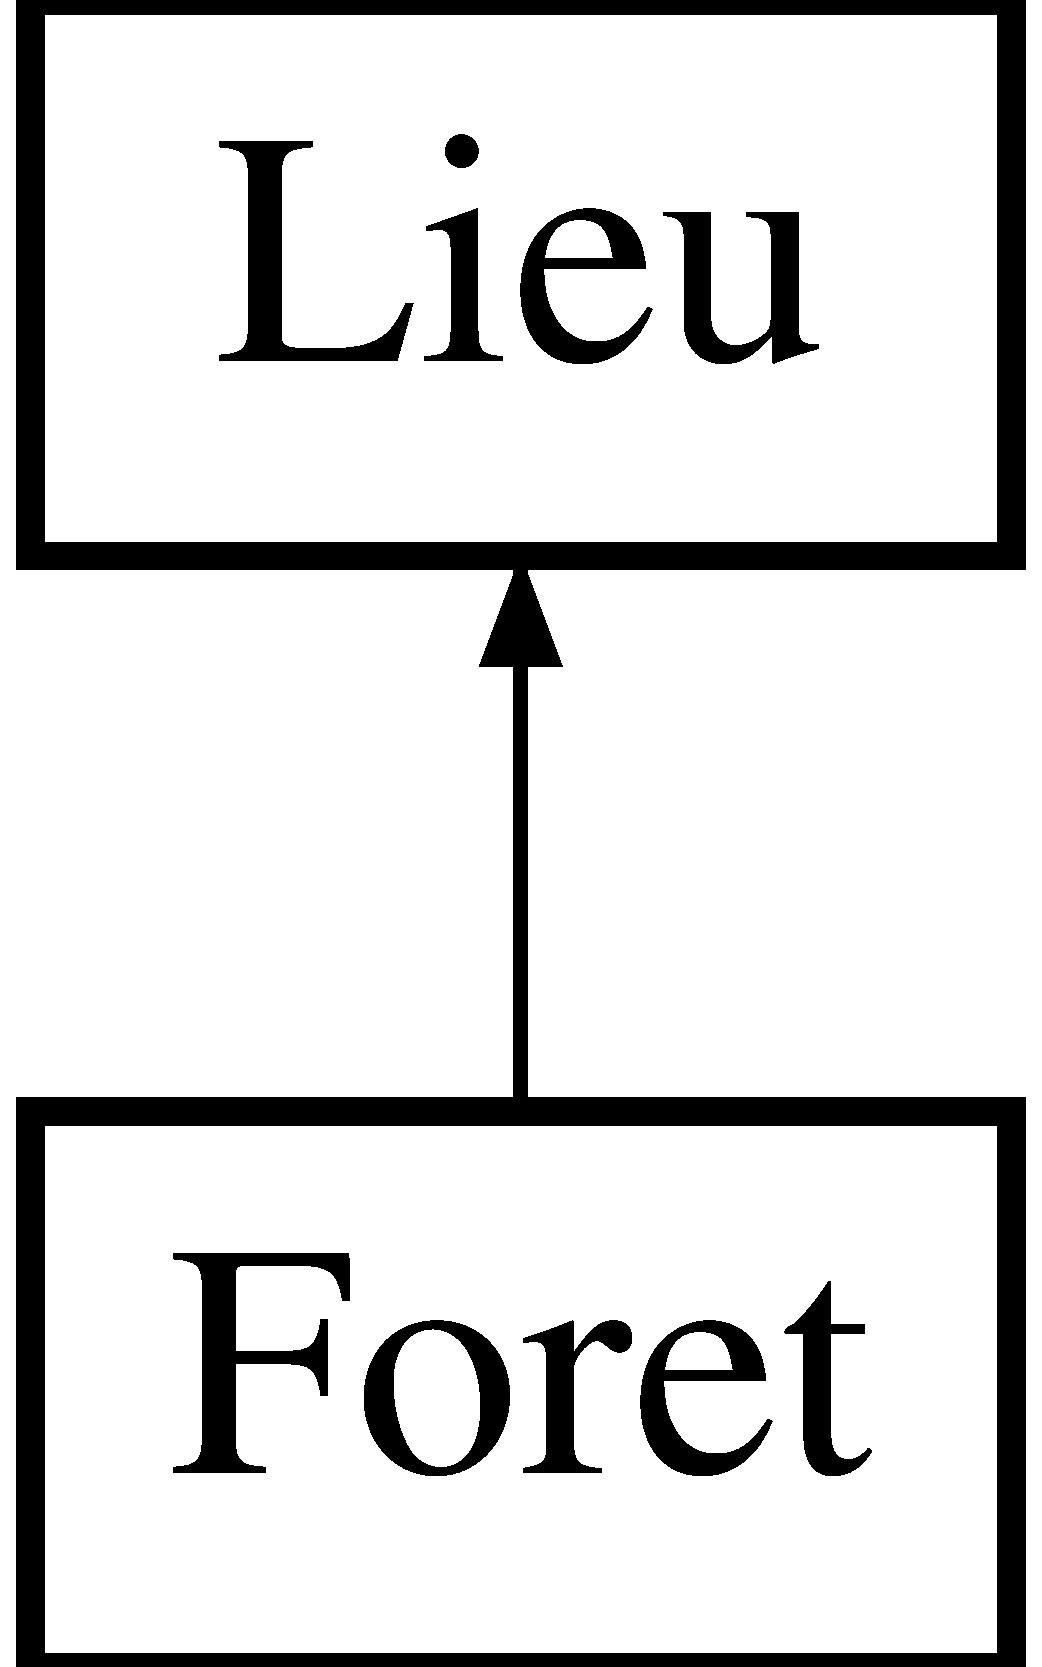
\includegraphics[height=2.000000cm]{class_foret}
\end{center}
\end{figure}
\subsection*{Public Member Functions}
\begin{DoxyCompactItemize}
\item 
\hyperlink{class_foret_a02cdb9636edbf4c2c6e406290cfad4db}{Foret} ()
\begin{DoxyCompactList}\small\item\em Constructeur par défaut. \end{DoxyCompactList}\item 
\hyperlink{class_foret_a936e4958fb4c860f0eebcea8e3652de1}{Foret} (vector$<$ \hyperlink{class_objet}{Objet} $>$ \hyperlink{class_lieu_a3a65fbb8ecba3f2e265905730ad2e631}{objets\-Dispo}, int \hyperlink{class_lieu_a90b76b521f92a43626ccd29ed5a29f89}{cash\-Cache}, vector$<$ \hyperlink{class_p_n_j}{P\-N\-J} $>$ \hyperlink{class_lieu_a8c1e20b105f7972f22d8f16651de4ebd}{liste\-P\-N\-J}, string \hyperlink{class_lieu_a1e48889fe5c581f043b8bd77ca497fc7}{nom\-Lieu}, vector$<$ string $>$ action\-Vec)
\begin{DoxyCompactList}\small\item\em Constructeur de la classe foret. \end{DoxyCompactList}\item 
void \hyperlink{class_foret_a7bde97b50ed9be97d62f84fe4868d44f}{executer\-Action} (\hyperlink{class_jeu}{Jeu} jeu, \hyperlink{class_heros}{Heros} $\ast$heros, \hyperlink{class_ville}{Ville} $\ast$ville)
\begin{DoxyCompactList}\small\item\em Exécute une action parmi les actions possibles comme parler à un \hyperlink{class_p_n_j}{P\-N\-J}, Fouiller, Afficher sac, Afficher stats du héros. \end{DoxyCompactList}\end{DoxyCompactItemize}
\subsection*{Additional Inherited Members}


\subsection{Detailed Description}
Classe représentant la foret. 

\subsection{Constructor \& Destructor Documentation}
\hypertarget{class_foret_a02cdb9636edbf4c2c6e406290cfad4db}{\index{Foret@{Foret}!Foret@{Foret}}
\index{Foret@{Foret}!Foret@{Foret}}
\subsubsection[{Foret}]{\setlength{\rightskip}{0pt plus 5cm}Foret\-::\-Foret (
\begin{DoxyParamCaption}
{}
\end{DoxyParamCaption}
)}}\label{class_foret_a02cdb9636edbf4c2c6e406290cfad4db}


Constructeur par défaut. 


\begin{DoxyCode}
19 \{\}
\end{DoxyCode}
\hypertarget{class_foret_a936e4958fb4c860f0eebcea8e3652de1}{\index{Foret@{Foret}!Foret@{Foret}}
\index{Foret@{Foret}!Foret@{Foret}}
\subsubsection[{Foret}]{\setlength{\rightskip}{0pt plus 5cm}Foret\-::\-Foret (
\begin{DoxyParamCaption}
\item[{vector$<$ {\bf Objet} $>$}]{objets\-Dispo, }
\item[{int}]{cash\-Cache, }
\item[{vector$<$ {\bf P\-N\-J} $>$}]{liste\-P\-N\-J, }
\item[{string}]{nom\-Lieu, }
\item[{vector$<$ string $>$}]{action\-Vec}
\end{DoxyParamCaption}
)}}\label{class_foret_a936e4958fb4c860f0eebcea8e3652de1}


Constructeur de la classe foret. 


\begin{DoxyParams}{Parameters}
{\em objets\-Dispo} & Le vecteur des objets disponibles dans la foret. \\
\hline
{\em cashcache} & La valeur du cash caché dans la foret. \\
\hline
{\em liste\-P\-N\-J} & Le vecteur des \hyperlink{class_p_n_j}{P\-N\-J} présents dans la foret. \\
\hline
{\em nom\-Lieu} & Le nom de la foret. \\
\hline
{\em action\-Vec} & Le vecteur des actions possibles dans la foret. \\
\hline
\end{DoxyParams}

\begin{DoxyCode}
20                                                                                                            
                   : \hyperlink{class_lieu_a0b3086d598fc1bfc0b4c09ae96304b3a}{Lieu} (\hyperlink{class_lieu_a3a65fbb8ecba3f2e265905730ad2e631}{objetsDispo}, \hyperlink{class_lieu_a90b76b521f92a43626ccd29ed5a29f89}{cashCache}, \hyperlink{class_lieu_a8c1e20b105f7972f22d8f16651de4ebd}{listePNJ}, \textcolor{stringliteral}{"Foret"}, actionVec)\{
21     \}
\end{DoxyCode}


\subsection{Member Function Documentation}
\hypertarget{class_foret_a7bde97b50ed9be97d62f84fe4868d44f}{\index{Foret@{Foret}!executer\-Action@{executer\-Action}}
\index{executer\-Action@{executer\-Action}!Foret@{Foret}}
\subsubsection[{executer\-Action}]{\setlength{\rightskip}{0pt plus 5cm}void Foret\-::executer\-Action (
\begin{DoxyParamCaption}
\item[{{\bf Jeu}}]{jeu, }
\item[{{\bf Heros} $\ast$}]{heros, }
\item[{{\bf Ville} $\ast$}]{ville}
\end{DoxyParamCaption}
)\hspace{0.3cm}{\ttfamily [virtual]}}}\label{class_foret_a7bde97b50ed9be97d62f84fe4868d44f}


Exécute une action parmi les actions possibles comme parler à un \hyperlink{class_p_n_j}{P\-N\-J}, Fouiller, Afficher sac, Afficher stats du héros. 


\begin{DoxyParams}{Parameters}
{\em jeu} & Une instance de la classe \hyperlink{class_jeu}{Jeu}. \\
\hline
{\em heros} & Un pointeur sur la classe \hyperlink{class_heros}{Heros}. \\
\hline
{\em ville} & Un pointeur sur la classe \hyperlink{class_ville}{Ville}. \\
\hline
\end{DoxyParams}


Reimplemented from \hyperlink{class_lieu_ad5d4e14283df04f0174f090f1614225c}{Lieu}.


\begin{DoxyCode}
35                                                                   \{
36 
37         \textcolor{keywordtype}{int} i=0, entree = -1 ;
38     \textcolor{keywordflow}{while} (entree!=i+3) \{
39 
40         jeu.\hyperlink{class_jeu_aa09fb40439f16b9665a0d76679f78e4e}{afficherTexte}( \textcolor{stringliteral}{"Vous êtes dans le lieu suivant : "} + 
      \hyperlink{class_lieu_a1e48889fe5c581f043b8bd77ca497fc7}{nomLieu} + \textcolor{stringliteral}{". Que voulez-vous faire ? (entrée attendue : un numéro)"} );
41 
42 
43         \textcolor{keywordflow}{for} (i=0 ; i < \hyperlink{class_lieu_a8c1e20b105f7972f22d8f16651de4ebd}{listePNJ}.size(); i++) \{
44 
45         jeu.\hyperlink{class_jeu_aa09fb40439f16b9665a0d76679f78e4e}{afficherTexte}(\hyperlink{foret_8cpp_a0d2f37137ee1fd6ff4a0ef803849dd63}{SSTR}(i) + \textcolor{stringliteral}{". Parler à la personne suivante :"} + 
      \hyperlink{class_lieu_a8c1e20b105f7972f22d8f16651de4ebd}{listePNJ}.at(i).getNom() );
46         \}
47 
48         jeu.\hyperlink{class_jeu_aa09fb40439f16b9665a0d76679f78e4e}{afficherTexte}(\hyperlink{foret_8cpp_a0d2f37137ee1fd6ff4a0ef803849dd63}{SSTR}(i) + \textcolor{stringliteral}{". "} + \textcolor{stringliteral}{"Fouiller"} );
49 
50         jeu.\hyperlink{class_jeu_aa09fb40439f16b9665a0d76679f78e4e}{afficherTexte}(\hyperlink{foret_8cpp_a0d2f37137ee1fd6ff4a0ef803849dd63}{SSTR}(i+1) + \textcolor{stringliteral}{". "} + \textcolor{stringliteral}{"Afficher Sac"} );
51 
52         jeu.\hyperlink{class_jeu_aa09fb40439f16b9665a0d76679f78e4e}{afficherTexte}(\hyperlink{foret_8cpp_a0d2f37137ee1fd6ff4a0ef803849dd63}{SSTR}(i+2) + \textcolor{stringliteral}{". "} + \textcolor{stringliteral}{"Afficher Stats du Héros"} );
53 
54         jeu.\hyperlink{class_jeu_aa09fb40439f16b9665a0d76679f78e4e}{afficherTexte}(\hyperlink{foret_8cpp_a0d2f37137ee1fd6ff4a0ef803849dd63}{SSTR}(i+3) + \textcolor{stringliteral}{". "} + \textcolor{stringliteral}{"Quitter"} );
55 
56 
57 
58         entree = jeu.\hyperlink{class_jeu_ac504a2a26ad7aa3c4281f8ab40cdc445}{demanderEntreeUtilisateur}(\textcolor{stringliteral}{"Faites votre choix :"});
59         \textcolor{keywordflow}{while} (entree < 0 or entree > i+3) \{
60             entree = jeu.\hyperlink{class_jeu_ac504a2a26ad7aa3c4281f8ab40cdc445}{demanderEntreeUtilisateur}(\textcolor{stringliteral}{"Faites un choix CORRECT :"});
61         \}
62 
63         \textcolor{keywordflow}{if} ( entree >= 0 and entree < i )
64             jeu.\hyperlink{class_jeu_aa09fb40439f16b9665a0d76679f78e4e}{afficherTexte}( heros->\hyperlink{class_heros_a4052af6e407ebdf4918e62340d374829}{ParleAPNJ}(&\hyperlink{class_lieu_a8c1e20b105f7972f22d8f16651de4ebd}{listePNJ}.at(entree), jeu) ) 
      ;
65 
66         \textcolor{keywordflow}{else} \textcolor{keywordflow}{if} ( entree == i )\{
67 
68             \hyperlink{class_lieu_a90d7fd86c93e59830e20156ddb7aeb50}{fouiller}(jeu, heros);
69 
70         \}
71 
72         \textcolor{keywordflow}{else} \textcolor{keywordflow}{if} ( entree == i+1 )\{
73 
74             jeu.\hyperlink{class_jeu_a26c7a428a96b1f987150cb708fa7d903}{consommersac}(heros);
75 
76         \}
77 
78         \textcolor{keywordflow}{else} \textcolor{keywordflow}{if} ( entree == i+2 )\{
79 
80             jeu.\hyperlink{class_jeu_a7f9e3b8e6f3ad5d2c47ae29c54f2bdc4}{affichageStatsHero}(*heros);
81 
82         \}
83 
84         \textcolor{keywordflow}{else} \textcolor{keywordflow}{if} ( entree == i+3 )\{
85             jeu.\hyperlink{class_jeu_a52ce4fb6c415b45209db13a589c9d675}{timer}(4, \textcolor{stringliteral}{"retour à la ville"});
86             heros->\hyperlink{class_heros_a8decc0b04f6724de10d2e2a8d1c3395c}{setLieuActuel}(ville);
87 
88         \}
89 
90         \textcolor{keywordflow}{else} \{\}
91 
92 
93     \}
94     
95     
96     \}
\end{DoxyCode}


The documentation for this class was generated from the following files\-:\begin{DoxyCompactItemize}
\item 
/nfs/usersgm/\-G\-M26/neljibbawe/\-Bureau/\-Projet\-C\-P\-P\-A\-Rendre/\-C\-P\-P R\-P\-G/\-R\-P\-G/\hyperlink{foret_8hpp}{foret.\-hpp}\item 
/nfs/usersgm/\-G\-M26/neljibbawe/\-Bureau/\-Projet\-C\-P\-P\-A\-Rendre/\-C\-P\-P R\-P\-G/\-R\-P\-G/\hyperlink{foret_8cpp}{foret.\-cpp}\end{DoxyCompactItemize}

\hypertarget{class_heros}{\section{Heros Class Reference}
\label{class_heros}\index{Heros@{Heros}}
}


Classe représentant l'héros.  




{\ttfamily \#include $<$heros.\-hpp$>$}

Inheritance diagram for Heros\-:\begin{figure}[H]
\begin{center}
\leavevmode
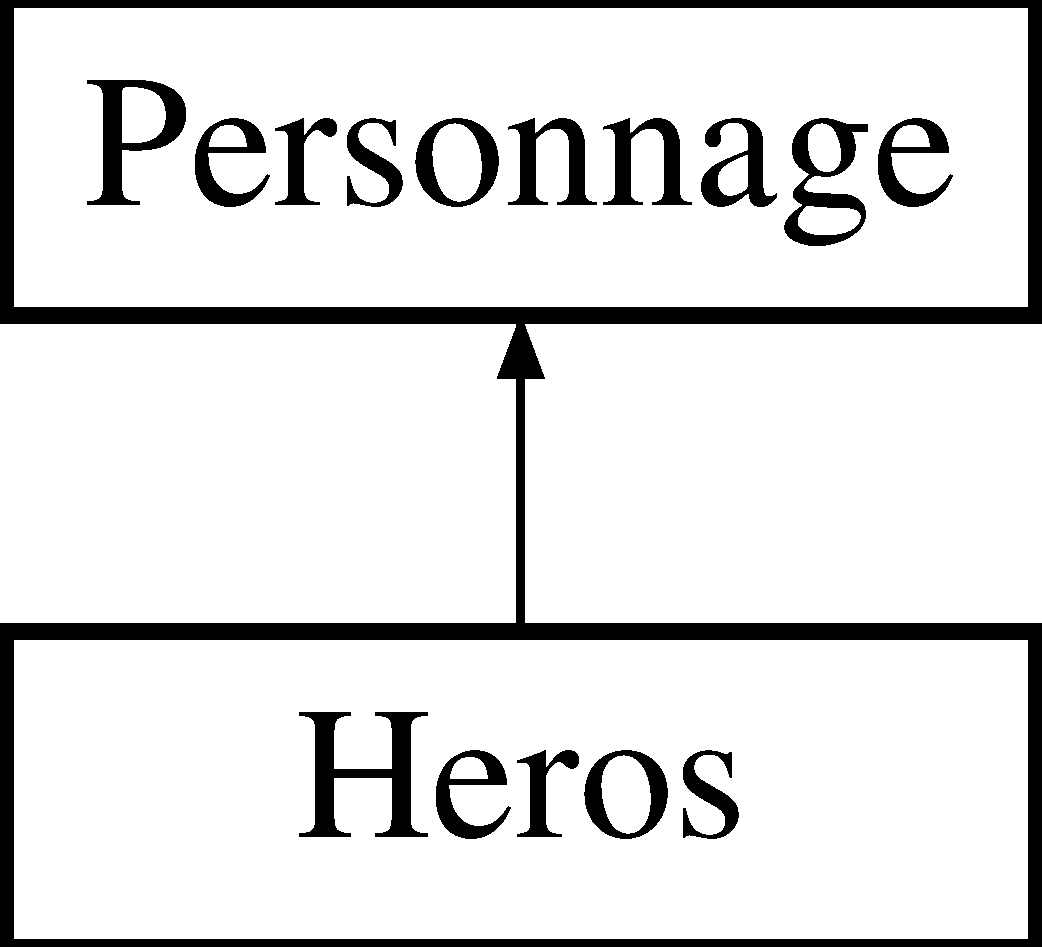
\includegraphics[height=2.000000cm]{class_heros}
\end{center}
\end{figure}
\subsection*{Public Member Functions}
\begin{DoxyCompactItemize}
\item 
\hyperlink{class_heros_ab4c8bc5b87a080c5f609a65bfab62c48}{Heros} ()
\begin{DoxyCompactList}\small\item\em Constructeur par défaut. \end{DoxyCompactList}\item 
\hyperlink{class_heros_a81e1ae1248debd353171ce44d910258d}{Heros} (int intelh, int forceh, int ageh, int cashh, int energieh, map$<$ string, \hyperlink{class_objet}{Objet} $\ast$ $>$sach, string nomh, vector$<$ \hyperlink{class_mission}{Mission} $\ast$ $>$ missh, \hyperlink{class_lieu}{Lieu} $\ast$lieuh)
\begin{DoxyCompactList}\small\item\em Constructeur de la classe \hyperlink{class_heros}{Heros}. \end{DoxyCompactList}\item 
vector$<$ \hyperlink{class_mission}{Mission} $\ast$ $>$ \hyperlink{class_heros_a38a959dcbaf42360236c0bb796ed7dcd}{mission\-Disponible} (\hyperlink{class_p_n_j}{P\-N\-J} $\ast$pnj)
\begin{DoxyCompactList}\small\item\em Retourne les missions disponibles proposées par les \hyperlink{class_p_n_j}{P\-N\-J}. \end{DoxyCompactList}\item 
void \hyperlink{class_heros_a88e91d926762f89d14b1bbc11ff4ae82}{se\-Deplacer} (\hyperlink{class_lieu}{Lieu} $\ast$lieu)
\begin{DoxyCompactList}\small\item\em Gère le déplacement de l'héros. \end{DoxyCompactList}\item 
\hyperlink{class_mission}{Mission} $\ast$ \hyperlink{class_heros_a11ebaa337de66722218930064505ce3c}{mission\-Plusaccess} (vector$<$ \hyperlink{class_mission}{Mission} $\ast$ $>$ miss)
\begin{DoxyCompactList}\small\item\em Sort la mission la plus adaptée à l'héros en fonction de ces statistiques. \end{DoxyCompactList}\item 
void \hyperlink{class_heros_ae87dba7afa03e7fdacfc3a7e82d3a6a3}{set\-Cash} (int new\-\_\-var)
\begin{DoxyCompactList}\small\item\em stock la valeur de la variable new\-\_\-var dans la variable cash. \end{DoxyCompactList}\item 
int \hyperlink{class_heros_a77bdee21cb8c8356448bb6669941441c}{get\-Cash} ()
\begin{DoxyCompactList}\small\item\em Accède à la variable cash. \end{DoxyCompactList}\item 
void \hyperlink{class_heros_a5d4f5d3d3a4db451923f0609a3e1b53c}{set\-Energie} (int new\-\_\-var)
\begin{DoxyCompactList}\small\item\em stock la valeur de la variable var dans la variable energie. \end{DoxyCompactList}\item 
int \hyperlink{class_heros_ae9bbef6d2edcb8b14d9ec3854146a42c}{get\-Energie} ()
\begin{DoxyCompactList}\small\item\em Accède à la variable energie. \end{DoxyCompactList}\item 
void \hyperlink{class_heros_a7d6d86388fe81deca1c5688ed07b2167}{set\-Sac} (map$<$ string, \hyperlink{class_objet}{Objet} $\ast$ $>$ new\-\_\-var)
\begin{DoxyCompactList}\small\item\em stock la valeur de la variable new\-\_\-var dans la variable sac. \end{DoxyCompactList}\item 
map$<$ string, \hyperlink{class_objet}{Objet} $\ast$ $>$ \hyperlink{class_heros_a62d8b172e82dbb0a1d2c23da21bdb069}{get\-Sac} ()
\begin{DoxyCompactList}\small\item\em Accède à la variable sac. \end{DoxyCompactList}\item 
void \hyperlink{class_heros_a74280cbf77bf35ee84728c989f6400c6}{set\-Nom\-Hero} (string new\-\_\-var)
\begin{DoxyCompactList}\small\item\em stock la valeur de la variable new\-\_\-var dans la variable nom\-Hero. \end{DoxyCompactList}\item 
string \hyperlink{class_heros_a1f950fc56d8c9813c4a7b76dae465478}{get\-Nom\-Hero} ()
\begin{DoxyCompactList}\small\item\em Accède à la variable nom\-Hero. \end{DoxyCompactList}\item 
void \hyperlink{class_heros_ae144c52184fc352808db4be369ced052}{set\-Missions} (vector$<$ \hyperlink{class_mission}{Mission} $\ast$ $>$ new\-\_\-var)
\begin{DoxyCompactList}\small\item\em stock la valeur de la variable new\-\_\-var dans la variable missions. \end{DoxyCompactList}\item 
vector$<$ \hyperlink{class_mission}{Mission} $\ast$ $>$ \hyperlink{class_heros_aae033294f652c209a599518e9a55fa83}{get\-Missions} ()
\begin{DoxyCompactList}\small\item\em Accède à la variable missions. \end{DoxyCompactList}\item 
void \hyperlink{class_heros_a8decc0b04f6724de10d2e2a8d1c3395c}{set\-Lieu\-Actuel} (\hyperlink{class_lieu}{Lieu} $\ast$new\-\_\-var)
\begin{DoxyCompactList}\small\item\em stock la valeur de la variable new\-\_\-var dans la variable lieu\-Actuel. \end{DoxyCompactList}\item 
\hyperlink{class_lieu}{Lieu} $\ast$ \hyperlink{class_heros_abb2a8141e5e2761b1eba4a902deca4ed}{get\-Lieu\-Actuel} ()
\begin{DoxyCompactList}\small\item\em Accède à la variable lieu\-Actuel. \end{DoxyCompactList}\item 
string \hyperlink{class_heros_a4052af6e407ebdf4918e62340d374829}{Parle\-A\-P\-N\-J} (\hyperlink{class_p_n_j}{P\-N\-J} $\ast$pnj, \hyperlink{class_jeu}{Jeu} jeu)
\begin{DoxyCompactList}\small\item\em Met en relation l'héros et les \hyperlink{class_p_n_j}{P\-N\-J}. \end{DoxyCompactList}\end{DoxyCompactItemize}
\subsection*{Additional Inherited Members}


\subsection{Detailed Description}
Classe représentant l'héros. 

\subsection{Constructor \& Destructor Documentation}
\hypertarget{class_heros_ab4c8bc5b87a080c5f609a65bfab62c48}{\index{Heros@{Heros}!Heros@{Heros}}
\index{Heros@{Heros}!Heros@{Heros}}
\subsubsection[{Heros}]{\setlength{\rightskip}{0pt plus 5cm}Heros\-::\-Heros (
\begin{DoxyParamCaption}
{}
\end{DoxyParamCaption}
)}}\label{class_heros_ab4c8bc5b87a080c5f609a65bfab62c48}


Constructeur par défaut. 


\begin{DoxyCode}
19 \{\}
\end{DoxyCode}
\hypertarget{class_heros_a81e1ae1248debd353171ce44d910258d}{\index{Heros@{Heros}!Heros@{Heros}}
\index{Heros@{Heros}!Heros@{Heros}}
\subsubsection[{Heros}]{\setlength{\rightskip}{0pt plus 5cm}Heros\-::\-Heros (
\begin{DoxyParamCaption}
\item[{int}]{intelh, }
\item[{int}]{forceh, }
\item[{int}]{ageh, }
\item[{int}]{cashh, }
\item[{int}]{energieh, }
\item[{map$<$ string, {\bf Objet} $\ast$ $>$}]{sach, }
\item[{string}]{nomh, }
\item[{vector$<$ {\bf Mission} $\ast$ $>$}]{missh, }
\item[{{\bf Lieu} $\ast$}]{lieuh}
\end{DoxyParamCaption}
)}}\label{class_heros_a81e1ae1248debd353171ce44d910258d}


Constructeur de la classe \hyperlink{class_heros}{Heros}. 


\begin{DoxyParams}{Parameters}
{\em intelh} & La valeur de l'intelligence de l'héros. \\
\hline
{\em forceh} & La valeur de la force de l'héros. \\
\hline
{\em ageh} & L'âge de l'héros. \\
\hline
{\em cashh} & La valeur du cash de l'héros. \\
\hline
{\em energieh} & La valeur de l'énergie de l'héros. \\
\hline
{\em sach} & Le sac d'objets de l'héros. \\
\hline
{\em nomh} & Le nom de l'héros. \\
\hline
{\em missh} & Le vecteur missions de l'héros. \\
\hline
{\em lieuh} & Un pointeur sur la classe \hyperlink{class_lieu}{Lieu}. \\
\hline
\end{DoxyParams}

\begin{DoxyCode}
22                                                                           :
      \hyperlink{class_personnage_abec36eb0310adc71f3375297fc590c65}{Personnage}
23 (intelh,forceh,ageh,nomh)\{
24         cash = cashh;
25         energie = energieh;
26         sac = sach;
27         missions = missh;
28         lieuActuel = lieuh; \}
\end{DoxyCode}


\subsection{Member Function Documentation}
\hypertarget{class_heros_a77bdee21cb8c8356448bb6669941441c}{\index{Heros@{Heros}!get\-Cash@{get\-Cash}}
\index{get\-Cash@{get\-Cash}!Heros@{Heros}}
\subsubsection[{get\-Cash}]{\setlength{\rightskip}{0pt plus 5cm}int Heros\-::get\-Cash (
\begin{DoxyParamCaption}
{}
\end{DoxyParamCaption}
)}}\label{class_heros_a77bdee21cb8c8356448bb6669941441c}


Accède à la variable cash. 

\begin{DoxyReturn}{Returns}
La valeur du cash de l'héros. 
\end{DoxyReturn}

\begin{DoxyCode}
57                         \{
58     \textcolor{keywordflow}{return} cash;
59   \}
\end{DoxyCode}
\hypertarget{class_heros_ae9bbef6d2edcb8b14d9ec3854146a42c}{\index{Heros@{Heros}!get\-Energie@{get\-Energie}}
\index{get\-Energie@{get\-Energie}!Heros@{Heros}}
\subsubsection[{get\-Energie}]{\setlength{\rightskip}{0pt plus 5cm}int Heros\-::get\-Energie (
\begin{DoxyParamCaption}
{}
\end{DoxyParamCaption}
)}}\label{class_heros_ae9bbef6d2edcb8b14d9ec3854146a42c}


Accède à la variable energie. 

\begin{DoxyReturn}{Returns}
La valeur de l'énergie de l'héros. 
\end{DoxyReturn}

\begin{DoxyCode}
66                            \{
67     \textcolor{keywordflow}{return} energie;
68   \}
\end{DoxyCode}
\hypertarget{class_heros_abb2a8141e5e2761b1eba4a902deca4ed}{\index{Heros@{Heros}!get\-Lieu\-Actuel@{get\-Lieu\-Actuel}}
\index{get\-Lieu\-Actuel@{get\-Lieu\-Actuel}!Heros@{Heros}}
\subsubsection[{get\-Lieu\-Actuel}]{\setlength{\rightskip}{0pt plus 5cm}{\bf Lieu} $\ast$ Heros\-::get\-Lieu\-Actuel (
\begin{DoxyParamCaption}
{}
\end{DoxyParamCaption}
)}}\label{class_heros_abb2a8141e5e2761b1eba4a902deca4ed}


Accède à la variable lieu\-Actuel. 

\begin{DoxyReturn}{Returns}
Un pointeur sur lieu. 
\end{DoxyReturn}

\begin{DoxyCode}
96                                 \{
97     \textcolor{keywordflow}{return} lieuActuel;
98   \}
\end{DoxyCode}
\hypertarget{class_heros_aae033294f652c209a599518e9a55fa83}{\index{Heros@{Heros}!get\-Missions@{get\-Missions}}
\index{get\-Missions@{get\-Missions}!Heros@{Heros}}
\subsubsection[{get\-Missions}]{\setlength{\rightskip}{0pt plus 5cm}vector$<$ {\bf Mission} $\ast$ $>$ Heros\-::get\-Missions (
\begin{DoxyParamCaption}
{}
\end{DoxyParamCaption}
)}}\label{class_heros_aae033294f652c209a599518e9a55fa83}


Accède à la variable missions. 

\begin{DoxyReturn}{Returns}
Le vecteur des missions de l'héros. 
\end{DoxyReturn}

\begin{DoxyCode}
87                                           \{
88     \textcolor{keywordflow}{return} missions;
89   \}
\end{DoxyCode}
\hypertarget{class_heros_a1f950fc56d8c9813c4a7b76dae465478}{\index{Heros@{Heros}!get\-Nom\-Hero@{get\-Nom\-Hero}}
\index{get\-Nom\-Hero@{get\-Nom\-Hero}!Heros@{Heros}}
\subsubsection[{get\-Nom\-Hero}]{\setlength{\rightskip}{0pt plus 5cm}string Heros\-::get\-Nom\-Hero (
\begin{DoxyParamCaption}
{}
\end{DoxyParamCaption}
)}}\label{class_heros_a1f950fc56d8c9813c4a7b76dae465478}


Accède à la variable nom\-Hero. 

\begin{DoxyReturn}{Returns}
Le nom de l'héros. 
\end{DoxyReturn}

\begin{DoxyCode}
30                         \{
31         \textcolor{keywordflow}{return} \hyperlink{class_personnage_acb7331b96dfc9f2aec78c60799030302}{nom};
32 \}
\end{DoxyCode}
\hypertarget{class_heros_a62d8b172e82dbb0a1d2c23da21bdb069}{\index{Heros@{Heros}!get\-Sac@{get\-Sac}}
\index{get\-Sac@{get\-Sac}!Heros@{Heros}}
\subsubsection[{get\-Sac}]{\setlength{\rightskip}{0pt plus 5cm}map$<$ string, {\bf Objet} $\ast$ $>$ Heros\-::get\-Sac (
\begin{DoxyParamCaption}
{}
\end{DoxyParamCaption}
)}}\label{class_heros_a62d8b172e82dbb0a1d2c23da21bdb069}


Accède à la variable sac. 

\begin{DoxyReturn}{Returns}
Un map constitué d'objets et leurs noms. 
\end{DoxyReturn}

\begin{DoxyCode}
77                                       \{
78     \textcolor{keywordflow}{return} sac;
79   \}
\end{DoxyCode}
\hypertarget{class_heros_a38a959dcbaf42360236c0bb796ed7dcd}{\index{Heros@{Heros}!mission\-Disponible@{mission\-Disponible}}
\index{mission\-Disponible@{mission\-Disponible}!Heros@{Heros}}
\subsubsection[{mission\-Disponible}]{\setlength{\rightskip}{0pt plus 5cm}vector$<$ {\bf Mission} $\ast$ $>$ Heros\-::mission\-Disponible (
\begin{DoxyParamCaption}
\item[{{\bf P\-N\-J} $\ast$}]{pnj}
\end{DoxyParamCaption}
)}}\label{class_heros_a38a959dcbaf42360236c0bb796ed7dcd}


Retourne les missions disponibles proposées par les \hyperlink{class_p_n_j}{P\-N\-J}. 


\begin{DoxyParams}{Parameters}
{\em pnj} & Un pointeur sur la classe \hyperlink{class_p_n_j}{P\-N\-J}. \\
\hline
\end{DoxyParams}
\begin{DoxyReturn}{Returns}
Le vecteur des missions disponibles. 
\end{DoxyReturn}

\begin{DoxyCode}
37                                                    \{
38 vector<Mission*> miss;
39 \textcolor{keywordflow}{for}(\textcolor{keywordtype}{int} i=0; i<pnj->\hyperlink{class_p_n_j_ab947fafa6afecf6640e1279ff05b7941}{getMissionsP}().size(); i++)\{
40         \textcolor{keywordflow}{if}(pnj->\hyperlink{class_p_n_j_ab947fafa6afecf6640e1279ff05b7941}{getMissionsP}().at(i)->getAccessIntel() <= 
      \hyperlink{class_personnage_a8e9bc213349fb0553d76d4da6a711231}{intelligence}
41                 && pnj->\hyperlink{class_p_n_j_ab947fafa6afecf6640e1279ff05b7941}{getMissionsP}().at(i)->getAccessForce () <= 
      \hyperlink{class_personnage_a823cd88582efee2ea29d199f96dcc677}{force}
42                 && pnj->\hyperlink{class_p_n_j_ab947fafa6afecf6640e1279ff05b7941}{getMissionsP}().at(i)->getAccessAge() <= \hyperlink{class_personnage_a2aa943e3c255f221eb9e57e8d134641f}{age} && pnj->
      \hyperlink{class_p_n_j_ab947fafa6afecf6640e1279ff05b7941}{getMissionsP}().at(i)->getEtatMission()!=\hyperlink{mission_8hpp_ace9df1e8554ba5a57340fb42cee370f7a9e765bd835523da043a754ce21905cb5}{achevee})
43 
44             miss.push\_back(pnj->\hyperlink{class_p_n_j_ab947fafa6afecf6640e1279ff05b7941}{getMissionsP}().at(i));
45         \}
46 \textcolor{keywordflow}{return} miss;
47 \}
\end{DoxyCode}
\hypertarget{class_heros_a11ebaa337de66722218930064505ce3c}{\index{Heros@{Heros}!mission\-Plusaccess@{mission\-Plusaccess}}
\index{mission\-Plusaccess@{mission\-Plusaccess}!Heros@{Heros}}
\subsubsection[{mission\-Plusaccess}]{\setlength{\rightskip}{0pt plus 5cm}{\bf Mission} $\ast$ Heros\-::mission\-Plusaccess (
\begin{DoxyParamCaption}
\item[{vector$<$ {\bf Mission} $\ast$ $>$}]{miss}
\end{DoxyParamCaption}
)}}\label{class_heros_a11ebaa337de66722218930064505ce3c}


Sort la mission la plus adaptée à l'héros en fonction de ces statistiques. 


\begin{DoxyParams}{Parameters}
{\em miss} & Un vecteur de missions. \\
\hline
\end{DoxyParams}
\begin{DoxyReturn}{Returns}
Un pointeur sur la classe \hyperlink{class_mission}{Mission}. 
\end{DoxyReturn}

\begin{DoxyCode}
102                                                       \{
103 \hyperlink{class_mission}{Mission} *min = (miss.at(0));
104         \textcolor{keywordflow}{for}(\textcolor{keywordtype}{int} i=0; i<miss.size(); i++)\{
105         \textcolor{keywordflow}{if}(miss.at(i)->getAccessIntel() + miss.at(i)->getAccessForce() +
106 miss.at(i)->getAccessAge() < min->\hyperlink{class_mission_ab3ed2d8bde3f15489406775cec6ca3ae}{getAccessIntel}() +
107 min->\hyperlink{class_mission_ae443e12738d9e3c52f27f3630df68bbf}{getAccessForce}() + min->\hyperlink{class_mission_a3ce0c4da70204a7bd84f9acb6306e43e}{getAccessAge}())
108                 min = miss.at(i);\}
109 \textcolor{keywordflow}{return} min;
110 \}
\end{DoxyCode}
\hypertarget{class_heros_a4052af6e407ebdf4918e62340d374829}{\index{Heros@{Heros}!Parle\-A\-P\-N\-J@{Parle\-A\-P\-N\-J}}
\index{Parle\-A\-P\-N\-J@{Parle\-A\-P\-N\-J}!Heros@{Heros}}
\subsubsection[{Parle\-A\-P\-N\-J}]{\setlength{\rightskip}{0pt plus 5cm}string Heros\-::\-Parle\-A\-P\-N\-J (
\begin{DoxyParamCaption}
\item[{{\bf P\-N\-J} $\ast$}]{pnj, }
\item[{{\bf Jeu}}]{jeu}
\end{DoxyParamCaption}
)}}\label{class_heros_a4052af6e407ebdf4918e62340d374829}


Met en relation l'héros et les \hyperlink{class_p_n_j}{P\-N\-J}. 


\begin{DoxyParams}{Parameters}
{\em pnj} & Un paramètre de la classe \hyperlink{class_p_n_j}{P\-N\-J}. \\
\hline
{\em jeu} & Un paramètre de la classe \hyperlink{class_jeu}{Jeu}. \\
\hline
\end{DoxyParams}
\begin{DoxyReturn}{Returns}
Un texte afin de gérer la communication entre l'héros et les pnj. 
\end{DoxyReturn}

\begin{DoxyCode}
113                                        \{
114         \textcolor{keywordflow}{if}(this->\hyperlink{class_heros_a38a959dcbaf42360236c0bb796ed7dcd}{missionDisponible}(pnj).empty())\{
115                 \textcolor{keywordflow}{return} pnj->\hyperlink{class_p_n_j_ac2495e0c6580568cd6299389df128b20}{getDialogueParDefaut}();\}
116             \textcolor{keywordflow}{else} \{
117                 \textcolor{keywordflow}{return} this->\hyperlink{class_heros_a11ebaa337de66722218930064505ce3c}{missionPlusaccess}( this->
      \hyperlink{class_heros_a38a959dcbaf42360236c0bb796ed7dcd}{missionDisponible}(pnj))->\hyperlink{class_mission_ad4375f925eda8637d6346ef468747f44}{executerMission}(jeu, \textcolor{keyword}{this}, pnj);
118             \}
119 \}
\end{DoxyCode}
\hypertarget{class_heros_a88e91d926762f89d14b1bbc11ff4ae82}{\index{Heros@{Heros}!se\-Deplacer@{se\-Deplacer}}
\index{se\-Deplacer@{se\-Deplacer}!Heros@{Heros}}
\subsubsection[{se\-Deplacer}]{\setlength{\rightskip}{0pt plus 5cm}void Heros\-::se\-Deplacer (
\begin{DoxyParamCaption}
\item[{{\bf Lieu} $\ast$}]{lieu}
\end{DoxyParamCaption}
)}}\label{class_heros_a88e91d926762f89d14b1bbc11ff4ae82}


Gère le déplacement de l'héros. 


\begin{DoxyParams}{Parameters}
{\em lieu} & Un pointeur sur la classe \hyperlink{class_lieu}{Lieu}. \\
\hline
\end{DoxyParams}

\begin{DoxyCode}
49                                  \{
50         lieuActuel = lieu;
51 \}
\end{DoxyCode}
\hypertarget{class_heros_ae87dba7afa03e7fdacfc3a7e82d3a6a3}{\index{Heros@{Heros}!set\-Cash@{set\-Cash}}
\index{set\-Cash@{set\-Cash}!Heros@{Heros}}
\subsubsection[{set\-Cash}]{\setlength{\rightskip}{0pt plus 5cm}void Heros\-::set\-Cash (
\begin{DoxyParamCaption}
\item[{int}]{new\-\_\-var}
\end{DoxyParamCaption}
)}}\label{class_heros_ae87dba7afa03e7fdacfc3a7e82d3a6a3}


stock la valeur de la variable new\-\_\-var dans la variable cash. 


\begin{DoxyCode}
53                                   \{
54       cash = new\_var;
55   \}
\end{DoxyCode}
\hypertarget{class_heros_a5d4f5d3d3a4db451923f0609a3e1b53c}{\index{Heros@{Heros}!set\-Energie@{set\-Energie}}
\index{set\-Energie@{set\-Energie}!Heros@{Heros}}
\subsubsection[{set\-Energie}]{\setlength{\rightskip}{0pt plus 5cm}void Heros\-::set\-Energie (
\begin{DoxyParamCaption}
\item[{int}]{new\-\_\-var}
\end{DoxyParamCaption}
)}}\label{class_heros_a5d4f5d3d3a4db451923f0609a3e1b53c}


stock la valeur de la variable var dans la variable energie. 


\begin{DoxyCode}
61                                        \{
62       energie = new\_var;
63   \}
\end{DoxyCode}
\hypertarget{class_heros_a8decc0b04f6724de10d2e2a8d1c3395c}{\index{Heros@{Heros}!set\-Lieu\-Actuel@{set\-Lieu\-Actuel}}
\index{set\-Lieu\-Actuel@{set\-Lieu\-Actuel}!Heros@{Heros}}
\subsubsection[{set\-Lieu\-Actuel}]{\setlength{\rightskip}{0pt plus 5cm}void Heros\-::set\-Lieu\-Actuel (
\begin{DoxyParamCaption}
\item[{{\bf Lieu} $\ast$}]{new\-\_\-var}
\end{DoxyParamCaption}
)}}\label{class_heros_a8decc0b04f6724de10d2e2a8d1c3395c}


stock la valeur de la variable new\-\_\-var dans la variable lieu\-Actuel. 


\begin{DoxyCode}
91                                             \{
92       lieuActuel = new\_var;
93   \}
\end{DoxyCode}
\hypertarget{class_heros_ae144c52184fc352808db4be369ced052}{\index{Heros@{Heros}!set\-Missions@{set\-Missions}}
\index{set\-Missions@{set\-Missions}!Heros@{Heros}}
\subsubsection[{set\-Missions}]{\setlength{\rightskip}{0pt plus 5cm}void Heros\-::set\-Missions (
\begin{DoxyParamCaption}
\item[{vector$<$ {\bf Mission} $\ast$ $>$}]{new\-\_\-var}
\end{DoxyParamCaption}
)}}\label{class_heros_ae144c52184fc352808db4be369ced052}


stock la valeur de la variable new\-\_\-var dans la variable missions. 


\begin{DoxyCode}
83                                                      \{
84       missions = new\_var;
85   \}
\end{DoxyCode}
\hypertarget{class_heros_a74280cbf77bf35ee84728c989f6400c6}{\index{Heros@{Heros}!set\-Nom\-Hero@{set\-Nom\-Hero}}
\index{set\-Nom\-Hero@{set\-Nom\-Hero}!Heros@{Heros}}
\subsubsection[{set\-Nom\-Hero}]{\setlength{\rightskip}{0pt plus 5cm}void Heros\-::set\-Nom\-Hero (
\begin{DoxyParamCaption}
\item[{string}]{new\-\_\-var}
\end{DoxyParamCaption}
)}}\label{class_heros_a74280cbf77bf35ee84728c989f6400c6}


stock la valeur de la variable new\-\_\-var dans la variable nom\-Hero. 


\begin{DoxyCode}
33                                  \{
34         \hyperlink{class_personnage_acb7331b96dfc9f2aec78c60799030302}{nom} = nomh;\}
\end{DoxyCode}
\hypertarget{class_heros_a7d6d86388fe81deca1c5688ed07b2167}{\index{Heros@{Heros}!set\-Sac@{set\-Sac}}
\index{set\-Sac@{set\-Sac}!Heros@{Heros}}
\subsubsection[{set\-Sac}]{\setlength{\rightskip}{0pt plus 5cm}void Heros\-::set\-Sac (
\begin{DoxyParamCaption}
\item[{map$<$ string, {\bf Objet} $\ast$ $>$}]{new\-\_\-var}
\end{DoxyParamCaption}
)}}\label{class_heros_a7d6d86388fe81deca1c5688ed07b2167}


stock la valeur de la variable new\-\_\-var dans la variable sac. 


\begin{DoxyCode}
72                                                   \{
73       sac = new\_var;
74   \}
\end{DoxyCode}


The documentation for this class was generated from the following files\-:\begin{DoxyCompactItemize}
\item 
/nfs/usersgm/\-G\-M26/neljibbawe/\-Bureau/\-Projet\-C\-P\-P\-A\-Rendre/\-C\-P\-P R\-P\-G/\-R\-P\-G/\hyperlink{heros_8hpp}{heros.\-hpp}\item 
/nfs/usersgm/\-G\-M26/neljibbawe/\-Bureau/\-Projet\-C\-P\-P\-A\-Rendre/\-C\-P\-P R\-P\-G/\-R\-P\-G/\hyperlink{heros_8cpp}{heros.\-cpp}\end{DoxyCompactItemize}

\hypertarget{class_jeu}{\section{Jeu Class Reference}
\label{class_jeu}\index{Jeu@{Jeu}}
}


Classe représentant le jeu.  




{\ttfamily \#include $<$jeu.\-hpp$>$}

\subsection*{Public Member Functions}
\begin{DoxyCompactItemize}
\item 
\hyperlink{class_jeu_acc5795ee00edf75516d3dfe65be3e6d6}{Jeu} ()
\begin{DoxyCompactList}\small\item\em Constructeur par défaut. \end{DoxyCompactList}\item 
void \hyperlink{class_jeu_ab049953d4de15842e4e3523c4323bc9e}{jouer} (\hyperlink{class_heros}{Heros} $\ast$heros, \hyperlink{class_ville}{Ville} $\ast$ville)
\begin{DoxyCompactList}\small\item\em Gère le jeu. \end{DoxyCompactList}\item 
void \hyperlink{class_jeu_a437282d939ce54d7f3e2eeb56dc0fce7}{initialiser\-Jeu} ()
\begin{DoxyCompactList}\small\item\em Initialise le jeu. \end{DoxyCompactList}\item 
bool \hyperlink{class_jeu_a3aa07b1e7a5e5d82479b8bb2a2841635}{demander\-Bool\-Utilisateur} (string texte)
\begin{DoxyCompactList}\small\item\em Vérifie si les saisies clavier faites par l'utilisateur sont correctes ou pas. \end{DoxyCompactList}\item 
int \hyperlink{class_jeu_ac504a2a26ad7aa3c4281f8ab40cdc445}{demander\-Entree\-Utilisateur} (string texte)
\begin{DoxyCompactList}\small\item\em Vérifie si les saisies clavier faites par l'utilisateur sont correctes ou pas. \end{DoxyCompactList}\item 
string \hyperlink{class_jeu_a4b70e906117c6a21b989ad3ab672c83c}{demander\-String\-Utilisateur} (string texte)
\begin{DoxyCompactList}\small\item\em Demande une saisie clavier à l'utilisateur sous forme d'un texte. \end{DoxyCompactList}\item 
void \hyperlink{class_jeu_aa09fb40439f16b9665a0d76679f78e4e}{afficher\-Texte} (string texte)
\begin{DoxyCompactList}\small\item\em Affiche le texte saisi par l'utilisateur. \end{DoxyCompactList}\item 
void \hyperlink{class_jeu_a26c7a428a96b1f987150cb708fa7d903}{consommersac} (\hyperlink{class_heros}{Heros} $\ast$heros)
\begin{DoxyCompactList}\small\item\em sert à consommer ou non un objet consommable par le héros. \end{DoxyCompactList}\item 
void \hyperlink{class_jeu_ac70f7bfb1945030e04287da3a35973af}{affichersac} (\hyperlink{class_heros}{Heros} $\ast$heros)
\begin{DoxyCompactList}\small\item\em Affiche le contenu du sac de l'héros. \end{DoxyCompactList}\item 
void \hyperlink{class_jeu_a52ce4fb6c415b45209db13a589c9d675}{timer} (int temps, string message)
\begin{DoxyCompactList}\small\item\em Gère le temps de déplacement de l'héros entre les différents lieux ou le temps d'une mission. \end{DoxyCompactList}\item 
void \hyperlink{class_jeu_a7f9e3b8e6f3ad5d2c47ae29c54f2bdc4}{affichage\-Stats\-Hero} (\hyperlink{class_heros}{Heros} heros)
\begin{DoxyCompactList}\small\item\em Affiche les stats de l'héros comme l'énergie, l'intelligence, le cash, la force et l'âge. \end{DoxyCompactList}\end{DoxyCompactItemize}


\subsection{Detailed Description}
Classe représentant le jeu. 

\subsection{Constructor \& Destructor Documentation}
\hypertarget{class_jeu_acc5795ee00edf75516d3dfe65be3e6d6}{\index{Jeu@{Jeu}!Jeu@{Jeu}}
\index{Jeu@{Jeu}!Jeu@{Jeu}}
\subsubsection[{Jeu}]{\setlength{\rightskip}{0pt plus 5cm}Jeu\-::\-Jeu (
\begin{DoxyParamCaption}
{}
\end{DoxyParamCaption}
)}}\label{class_jeu_acc5795ee00edf75516d3dfe65be3e6d6}


Constructeur par défaut. 


\begin{DoxyCode}
254         \{
255 
256 \}
\end{DoxyCode}


\subsection{Member Function Documentation}
\hypertarget{class_jeu_a7f9e3b8e6f3ad5d2c47ae29c54f2bdc4}{\index{Jeu@{Jeu}!affichage\-Stats\-Hero@{affichage\-Stats\-Hero}}
\index{affichage\-Stats\-Hero@{affichage\-Stats\-Hero}!Jeu@{Jeu}}
\subsubsection[{affichage\-Stats\-Hero}]{\setlength{\rightskip}{0pt plus 5cm}void Jeu\-::affichage\-Stats\-Hero (
\begin{DoxyParamCaption}
\item[{{\bf Heros}}]{heros}
\end{DoxyParamCaption}
)}}\label{class_jeu_a7f9e3b8e6f3ad5d2c47ae29c54f2bdc4}


Affiche les stats de l'héros comme l'énergie, l'intelligence, le cash, la force et l'âge. 


\begin{DoxyParams}{Parameters}
{\em heros} & Une instance de la classe \hyperlink{class_heros}{Heros}. \\
\hline
\end{DoxyParams}

\begin{DoxyCode}
374                                         \{
375     this->\hyperlink{class_jeu_aa09fb40439f16b9665a0d76679f78e4e}{afficherTexte}(\textcolor{stringliteral}{"Voici vos stats: Energie : "} + \hyperlink{jeu_8cpp_a0d2f37137ee1fd6ff4a0ef803849dd63}{SSTR}(heros.
      \hyperlink{class_heros_ae9bbef6d2edcb8b14d9ec3854146a42c}{getEnergie}()) + \textcolor{stringliteral}{"\(\backslash\)n"} + \textcolor{stringliteral}{"Intelligence : "} + \hyperlink{jeu_8cpp_a0d2f37137ee1fd6ff4a0ef803849dd63}{SSTR}(heros.
      \hyperlink{class_personnage_a250eec1aba0df7a105dd564e4cd02b0b}{getIntelligence}()) + \textcolor{stringliteral}{"\(\backslash\)n"} + \textcolor{stringliteral}{"Cash : "} + \hyperlink{jeu_8cpp_a0d2f37137ee1fd6ff4a0ef803849dd63}{SSTR}(heros.\hyperlink{class_heros_a77bdee21cb8c8356448bb6669941441c}{getCash}()) + \textcolor{stringliteral}{"\(\backslash\)n"} + \textcolor{stringliteral}{"Force : "}
       + \hyperlink{jeu_8cpp_a0d2f37137ee1fd6ff4a0ef803849dd63}{SSTR}(heros.\hyperlink{class_personnage_a40de0ba95f25eb6f1653b6a4183763ae}{getForce}()) + \textcolor{stringliteral}{"\(\backslash\)n"} + \textcolor{stringliteral}{"Age : "} + \hyperlink{jeu_8cpp_a0d2f37137ee1fd6ff4a0ef803849dd63}{SSTR}(heros.\hyperlink{class_personnage_a991d7e1cf4662e245ad72e76b9eb9d53}{getAge}()));
376     \hyperlink{class_jeu_a52ce4fb6c415b45209db13a589c9d675}{timer}(4,\textcolor{stringliteral}{""});
377 \}
\end{DoxyCode}
\hypertarget{class_jeu_ac70f7bfb1945030e04287da3a35973af}{\index{Jeu@{Jeu}!affichersac@{affichersac}}
\index{affichersac@{affichersac}!Jeu@{Jeu}}
\subsubsection[{affichersac}]{\setlength{\rightskip}{0pt plus 5cm}void Jeu\-::affichersac (
\begin{DoxyParamCaption}
\item[{{\bf Heros} $\ast$}]{heros}
\end{DoxyParamCaption}
)}}\label{class_jeu_ac70f7bfb1945030e04287da3a35973af}


Affiche le contenu du sac de l'héros. 


\begin{DoxyParams}{Parameters}
{\em heros} & Un pointeur sur la classe \hyperlink{class_heros}{Heros}. \\
\hline
\end{DoxyParams}

\begin{DoxyCode}
316                                  \{
317         \textcolor{keywordtype}{string} s ;
318         map <string, Objet*> sacH=heros->\hyperlink{class_heros_a62d8b172e82dbb0a1d2c23da21bdb069}{getSac}();
319 
320         \textcolor{keywordflow}{for}(map<string,Objet*>::iterator it=sacH.begin(); it!=sacH.end(); ++it) \{
321             \textcolor{keywordflow}{if}(it->second->getQuantiteObjet()>0) \{
322                 this->\hyperlink{class_jeu_aa09fb40439f16b9665a0d76679f78e4e}{afficherTexte}(\textcolor{stringliteral}{"- ("} + \hyperlink{jeu_8cpp_a0d2f37137ee1fd6ff4a0ef803849dd63}{SSTR}(it->second->getQuantiteObjet()) + \textcolor{stringliteral}{")"}
323 + it->first + \textcolor{stringliteral}{"\(\backslash\)n"} );
324                 \}
325 
326         \}
327 \}
\end{DoxyCode}
\hypertarget{class_jeu_aa09fb40439f16b9665a0d76679f78e4e}{\index{Jeu@{Jeu}!afficher\-Texte@{afficher\-Texte}}
\index{afficher\-Texte@{afficher\-Texte}!Jeu@{Jeu}}
\subsubsection[{afficher\-Texte}]{\setlength{\rightskip}{0pt plus 5cm}void Jeu\-::afficher\-Texte (
\begin{DoxyParamCaption}
\item[{string}]{texte}
\end{DoxyParamCaption}
)}}\label{class_jeu_aa09fb40439f16b9665a0d76679f78e4e}


Affiche le texte saisi par l'utilisateur. 


\begin{DoxyParams}{Parameters}
{\em texte} & Un texte demandé à l'utilisateur afin qu'il fasse son choix. \\
\hline
\end{DoxyParams}

\begin{DoxyCode}
312                                     \{
313     cout<<texte<<endl;
314 \}
\end{DoxyCode}
\hypertarget{class_jeu_a26c7a428a96b1f987150cb708fa7d903}{\index{Jeu@{Jeu}!consommersac@{consommersac}}
\index{consommersac@{consommersac}!Jeu@{Jeu}}
\subsubsection[{consommersac}]{\setlength{\rightskip}{0pt plus 5cm}void Jeu\-::consommersac (
\begin{DoxyParamCaption}
\item[{{\bf Heros} $\ast$}]{heros}
\end{DoxyParamCaption}
)}}\label{class_jeu_a26c7a428a96b1f987150cb708fa7d903}


sert à consommer ou non un objet consommable par le héros. 


\begin{DoxyParams}{Parameters}
{\em heros} & Un pointeur sur la classe \hyperlink{class_heros}{Heros}. \\
\hline
\end{DoxyParams}

\begin{DoxyCode}
330                                   \{
331         this->\hyperlink{class_jeu_aa09fb40439f16b9665a0d76679f78e4e}{afficherTexte}(\textcolor{stringliteral}{"Voici les objets dans le sac"});
332         this->\hyperlink{class_jeu_ac70f7bfb1945030e04287da3a35973af}{affichersac}(heros);
333         \textcolor{keywordflow}{if} (\hyperlink{class_jeu_a3aa07b1e7a5e5d82479b8bb2a2841635}{demanderBoolUtilisateur}(\textcolor{stringliteral}{"Consommer un objet ?"}))\{
334         map<string,Objet*> sac = heros->\hyperlink{class_heros_a62d8b172e82dbb0a1d2c23da21bdb069}{getSac}();
335         \textcolor{keywordtype}{string} choix1;
336         \textcolor{keywordflow}{do}\{
337          choix1 = this->\hyperlink{class_jeu_a4b70e906117c6a21b989ad3ab672c83c}{demanderStringUtilisateur}(\textcolor{stringliteral}{"Faites votre choix (écrivez le
       nom de l'objet tel qu'il est orthographié) ou 'q' pour quitter."});
338 
339          \textcolor{keywordflow}{if} (choix1==\textcolor{stringliteral}{"q"}) \{\textcolor{keywordflow}{return};\}
340          \textcolor{keywordflow}{else} \textcolor{keywordflow}{if}(sac.find(choix1) == sac.end())
341                                    \{this->\hyperlink{class_jeu_aa09fb40439f16b9665a0d76679f78e4e}{afficherTexte}(\textcolor{stringliteral}{"Veuillez choisir un objet consommable
      "});\}
342         \}\textcolor{keywordflow}{while}(sac.find(choix1) == sac.end() && choix1!=\textcolor{stringliteral}{"q"});
343 
344          \textcolor{keywordtype}{bool} choix2 = this->\hyperlink{class_jeu_a3aa07b1e7a5e5d82479b8bb2a2841635}{demanderBoolUtilisateur}(\textcolor{stringliteral}{"Consommer?"} );
345                  \textcolor{keywordflow}{if}(choix2 == 1)\{
346 
347                          sac[choix1]->setQuantiteObjet(sac[choix1]->getQuantiteObjet()-1);
348                          heros->\hyperlink{class_heros_a7d6d86388fe81deca1c5688ed07b2167}{setSac}(sac);
349 
350 
351                          sac[choix1]->utiliserObjet(*\textcolor{keyword}{this},heros);
352                  \}\textcolor{keywordflow}{else}
353                          this->\hyperlink{class_jeu_aa09fb40439f16b9665a0d76679f78e4e}{afficherTexte}(\textcolor{stringliteral}{"Vous avez choisi de ne pas consommer objet"});
354         \}
355         \textcolor{keywordflow}{else} \textcolor{keywordflow}{return};
356 
357 \}
\end{DoxyCode}
\hypertarget{class_jeu_a3aa07b1e7a5e5d82479b8bb2a2841635}{\index{Jeu@{Jeu}!demander\-Bool\-Utilisateur@{demander\-Bool\-Utilisateur}}
\index{demander\-Bool\-Utilisateur@{demander\-Bool\-Utilisateur}!Jeu@{Jeu}}
\subsubsection[{demander\-Bool\-Utilisateur}]{\setlength{\rightskip}{0pt plus 5cm}bool Jeu\-::demander\-Bool\-Utilisateur (
\begin{DoxyParamCaption}
\item[{string}]{texte}
\end{DoxyParamCaption}
)}}\label{class_jeu_a3aa07b1e7a5e5d82479b8bb2a2841635}


Vérifie si les saisies clavier faites par l'utilisateur sont correctes ou pas. 


\begin{DoxyParams}{Parameters}
{\em texte} & Un texte correspondant au choix de l'utilisateur. \\
\hline
\end{DoxyParams}
\begin{DoxyReturn}{Returns}
un booléen. 
\end{DoxyReturn}

\begin{DoxyCode}
262                                               \{
263 
264         \textcolor{keywordtype}{string} s;
265         \textcolor{keywordtype}{int} l;
266 
267         \textcolor{keywordtype}{bool} isInt=\textcolor{keyword}{false};
268 
269         cout<<texte<<endl<<\textcolor{stringliteral}{"1 : oui, 0 : non"}<<endl;
270         \textcolor{keywordflow}{do} \{
271             cin>>s;
272             istringstream istr(s);
273             isInt=(istr>>l);
274             \textcolor{keywordflow}{if} (!isInt or !(l==0 or l==1))
275                 cout << \textcolor{stringliteral}{"Entrée incorrecte, veuillez recommencer."} << endl ;
276         \}\textcolor{keywordflow}{while} (!isInt or !(l==0 or l==1));
277 
278         \textcolor{keywordflow}{if} (l==0)
279             \textcolor{keywordflow}{return} \textcolor{keyword}{false};
280         \textcolor{keywordflow}{else} \textcolor{keywordflow}{if} (l==1)
281             \textcolor{keywordflow}{return} \textcolor{keyword}{true};
282         \textcolor{keywordflow}{else}\{\}
283 
284 \}
\end{DoxyCode}
\hypertarget{class_jeu_ac504a2a26ad7aa3c4281f8ab40cdc445}{\index{Jeu@{Jeu}!demander\-Entree\-Utilisateur@{demander\-Entree\-Utilisateur}}
\index{demander\-Entree\-Utilisateur@{demander\-Entree\-Utilisateur}!Jeu@{Jeu}}
\subsubsection[{demander\-Entree\-Utilisateur}]{\setlength{\rightskip}{0pt plus 5cm}int Jeu\-::demander\-Entree\-Utilisateur (
\begin{DoxyParamCaption}
\item[{string}]{texte}
\end{DoxyParamCaption}
)}}\label{class_jeu_ac504a2a26ad7aa3c4281f8ab40cdc445}


Vérifie si les saisies clavier faites par l'utilisateur sont correctes ou pas. 


\begin{DoxyParams}{Parameters}
{\em texte} & Un texte correspondant au choix de l'utilisateur. \\
\hline
\end{DoxyParams}
\begin{DoxyReturn}{Returns}
un booléen. 
\end{DoxyReturn}

\begin{DoxyCode}
287                                                \{
288     \textcolor{keywordtype}{string} s;
289     \textcolor{keywordtype}{int} l;
290     \textcolor{keywordtype}{bool} isInt=\textcolor{keyword}{false};
291     cout<<texte<<endl;
292 
293     \textcolor{keywordflow}{do} \{
294         cin>>s;
295         istringstream istr(s);
296         isInt=(istr>>l);
297         \textcolor{keywordflow}{if} (!isInt)
298             cout << \textcolor{stringliteral}{"Entrée incorrecte, veuillez recommencer."} << endl ;
299     \}
300     \textcolor{keywordflow}{while} (!isInt);
301 
302     \textcolor{keywordflow}{return} l;
303 \}
\end{DoxyCode}
\hypertarget{class_jeu_a4b70e906117c6a21b989ad3ab672c83c}{\index{Jeu@{Jeu}!demander\-String\-Utilisateur@{demander\-String\-Utilisateur}}
\index{demander\-String\-Utilisateur@{demander\-String\-Utilisateur}!Jeu@{Jeu}}
\subsubsection[{demander\-String\-Utilisateur}]{\setlength{\rightskip}{0pt plus 5cm}string Jeu\-::demander\-String\-Utilisateur (
\begin{DoxyParamCaption}
\item[{string}]{texte}
\end{DoxyParamCaption}
)}}\label{class_jeu_a4b70e906117c6a21b989ad3ab672c83c}


Demande une saisie clavier à l'utilisateur sous forme d'un texte. 


\begin{DoxyParams}{Parameters}
{\em texte} & Un texte correspondant à la saisie clavier de l'utilisateur. \\
\hline
\end{DoxyParams}
\begin{DoxyReturn}{Returns}
un entier. 
\end{DoxyReturn}

\begin{DoxyCode}
305                                                   \{
306     cout<<texte<<endl;
307     \textcolor{keywordtype}{string} l;
308     cin>>l;
309     \textcolor{keywordflow}{return} l;
310 \}
\end{DoxyCode}
\hypertarget{class_jeu_a437282d939ce54d7f3e2eeb56dc0fce7}{\index{Jeu@{Jeu}!initialiser\-Jeu@{initialiser\-Jeu}}
\index{initialiser\-Jeu@{initialiser\-Jeu}!Jeu@{Jeu}}
\subsubsection[{initialiser\-Jeu}]{\setlength{\rightskip}{0pt plus 5cm}void Jeu\-::initialiser\-Jeu (
\begin{DoxyParamCaption}
{}
\end{DoxyParamCaption}
)}}\label{class_jeu_a437282d939ce54d7f3e2eeb56dc0fce7}


Initialise le jeu. 


\begin{DoxyCode}
258                         \{
259 
260 \} 
\end{DoxyCode}
\hypertarget{class_jeu_ab049953d4de15842e4e3523c4323bc9e}{\index{Jeu@{Jeu}!jouer@{jouer}}
\index{jouer@{jouer}!Jeu@{Jeu}}
\subsubsection[{jouer}]{\setlength{\rightskip}{0pt plus 5cm}void Jeu\-::jouer (
\begin{DoxyParamCaption}
\item[{{\bf Heros} $\ast$}]{heros, }
\item[{{\bf Ville} $\ast$}]{ville}
\end{DoxyParamCaption}
)}}\label{class_jeu_ab049953d4de15842e4e3523c4323bc9e}


Gère le jeu. 


\begin{DoxyParams}{Parameters}
{\em heros} & Un pointeur sur la classe \hyperlink{class_heros}{Heros}. \\
\hline
{\em ville} & Un pointeur sur la classe \hyperlink{class_ville}{Ville}. \\
\hline
\end{DoxyParams}

\begin{DoxyCode}
242                                          \{
243 
244     \textcolor{keywordflow}{while}(heros->\hyperlink{class_personnage_a250eec1aba0df7a105dd564e4cd02b0b}{getIntelligence}() < \hyperlink{jeu_8cpp_a9d6989b85af84d4c359c8a47437cf8b7}{INTELFIN} || heros->
      \hyperlink{class_personnage_a40de0ba95f25eb6f1653b6a4183763ae}{getForce}() < \hyperlink{jeu_8cpp_ab33c269a96a182fa40c46ae8f0eec850}{FORCEFIN} )\{
245         heros->\hyperlink{class_heros_abb2a8141e5e2761b1eba4a902deca4ed}{getLieuActuel}()->\hyperlink{class_lieu_ad5d4e14283df04f0174f090f1614225c}{executerAction}(*\textcolor{keyword}{this}, heros, ville);
246     \}
247 
248     \textcolor{keywordflow}{if}(heros->\hyperlink{class_personnage_a250eec1aba0df7a105dd564e4cd02b0b}{getIntelligence}()>=\hyperlink{jeu_8cpp_a9d6989b85af84d4c359c8a47437cf8b7}{INTELFIN} )\{
249         \hyperlink{class_jeu_aa09fb40439f16b9665a0d76679f78e4e}{afficherTexte}(\textcolor{stringliteral}{"Bravo, vous avez terminé le jeu, vous avez atteint "}+
      \hyperlink{jeu_8cpp_a0d2f37137ee1fd6ff4a0ef803849dd63}{SSTR}(\hyperlink{jeu_8cpp_a9d6989b85af84d4c359c8a47437cf8b7}{INTELFIN})+\textcolor{stringliteral}{" d'intelligence, vous avez le droit à une banane !"});
250     \}
251 \}
\end{DoxyCode}
\hypertarget{class_jeu_a52ce4fb6c415b45209db13a589c9d675}{\index{Jeu@{Jeu}!timer@{timer}}
\index{timer@{timer}!Jeu@{Jeu}}
\subsubsection[{timer}]{\setlength{\rightskip}{0pt plus 5cm}void Jeu\-::timer (
\begin{DoxyParamCaption}
\item[{int}]{temps, }
\item[{string}]{message}
\end{DoxyParamCaption}
)}}\label{class_jeu_a52ce4fb6c415b45209db13a589c9d675}


Gère le temps de déplacement de l'héros entre les différents lieux ou le temps d'une mission. 


\begin{DoxyParams}{Parameters}
{\em temps} & Un temps correspondant à la durée du timer. \\
\hline
{\em message} & Un texte permettant de savoir ce qui est en train de se passer pendant le temps temps. \\
\hline
\end{DoxyParams}

\begin{DoxyCode}
360                                         \{
361     time\_t \hyperlink{class_jeu_a52ce4fb6c415b45209db13a589c9d675}{timer};
362     \textcolor{keywordtype}{double} t =time(&timer);
363     \hyperlink{class_jeu_aa09fb40439f16b9665a0d76679f78e4e}{afficherTexte}(message);
364     \textcolor{keywordtype}{int} i=1;
365     \textcolor{keywordflow}{while}(time(&timer)-t<temps) \{
366         \textcolor{keywordflow}{if} (time(&timer)-t == i)\{
367             cout<<\textcolor{stringliteral}{"."}<<endl;
368             i++;
369         \}
370     \}
371     \textcolor{keywordflow}{return};
372 \}
\end{DoxyCode}


The documentation for this class was generated from the following files\-:\begin{DoxyCompactItemize}
\item 
/nfs/usersgm/\-G\-M26/neljibbawe/\-Bureau/\-Projet\-C\-P\-P\-A\-Rendre/\-C\-P\-P R\-P\-G/\-R\-P\-G/\hyperlink{jeu_8hpp}{jeu.\-hpp}\item 
/nfs/usersgm/\-G\-M26/neljibbawe/\-Bureau/\-Projet\-C\-P\-P\-A\-Rendre/\-C\-P\-P R\-P\-G/\-R\-P\-G/\hyperlink{jeu_8cpp}{jeu.\-cpp}\end{DoxyCompactItemize}

\hypertarget{class_lieu}{\section{Lieu Class Reference}
\label{class_lieu}\index{Lieu@{Lieu}}
}


Classe représentant le lieu.  




{\ttfamily \#include $<$lieu.\-hpp$>$}

Inheritance diagram for Lieu\-:\begin{figure}[H]
\begin{center}
\leavevmode
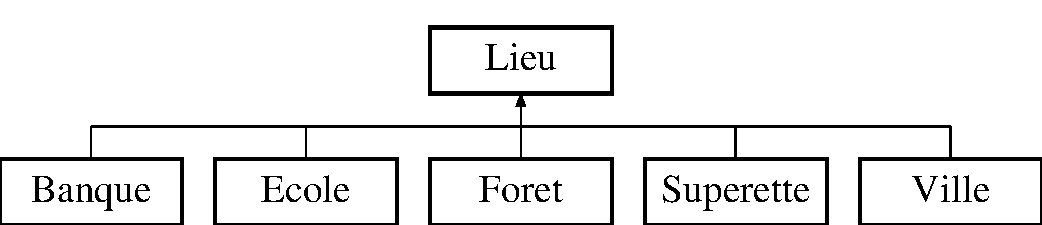
\includegraphics[height=2.000000cm]{class_lieu}
\end{center}
\end{figure}
\subsection*{Public Member Functions}
\begin{DoxyCompactItemize}
\item 
\hyperlink{class_lieu_a0b3086d598fc1bfc0b4c09ae96304b3a}{Lieu} ()
\begin{DoxyCompactList}\small\item\em Constructeur par défaut. \end{DoxyCompactList}\item 
\hyperlink{class_lieu_abb644ef90d500f7b6d7d110b1dc06896}{Lieu} (vector$<$ \hyperlink{class_objet}{Objet} $>$ \hyperlink{class_lieu_a3a65fbb8ecba3f2e265905730ad2e631}{objets\-Dispo}, int \hyperlink{class_lieu_a90b76b521f92a43626ccd29ed5a29f89}{cash\-Cache}, vector$<$ \hyperlink{class_p_n_j}{P\-N\-J} $>$ \hyperlink{class_lieu_a8c1e20b105f7972f22d8f16651de4ebd}{liste\-P\-N\-J}, string \hyperlink{class_lieu_a1e48889fe5c581f043b8bd77ca497fc7}{nom\-Lieu}, vector$<$ string $>$ action\-Vec)
\begin{DoxyCompactList}\small\item\em Constructeur de la classe lieu. \end{DoxyCompactList}\item 
virtual \hyperlink{class_lieu_af0e191bcc85454c9e59d107cfb557b20}{$\sim$\-Lieu} ()
\begin{DoxyCompactList}\small\item\em Destructeur par défaut. \end{DoxyCompactList}\item 
void \hyperlink{class_lieu_a7af4284fb6e898e2ef29ad06ea244cc0}{set\-Objets\-Dispo} (vector$<$ \hyperlink{class_objet}{Objet} $>$ new\-\_\-var)
\begin{DoxyCompactList}\small\item\em stock la valeur de la variable new\-\_\-var dans la variable objets\-Dispo. \end{DoxyCompactList}\item 
vector$<$ \hyperlink{class_objet}{Objet} $>$ \hyperlink{class_lieu_ad4fbedc5d8b53c0b79684aa34c6700b8}{get\-Objets\-Dispo} () const 
\begin{DoxyCompactList}\small\item\em Accède à la variable objets\-Dispo. \end{DoxyCompactList}\item 
void \hyperlink{class_lieu_af9efb050ea38c72ad7d7bc7e2f128875}{set\-Liste\-P\-N\-J} (vector$<$ \hyperlink{class_p_n_j}{P\-N\-J} $>$ new\-\_\-var)
\begin{DoxyCompactList}\small\item\em stock la valeur de la variable new\-\_\-var dans la variable liste\-P\-N\-J. \end{DoxyCompactList}\item 
vector$<$ \hyperlink{class_p_n_j}{P\-N\-J} $>$ \hyperlink{class_lieu_abfe724c1e50380a4a4c2d5b522dc60d2}{get\-Liste\-P\-N\-J} () const 
\begin{DoxyCompactList}\small\item\em Accède à la variable liste\-P\-N\-J. \end{DoxyCompactList}\item 
void \hyperlink{class_lieu_a13f53069b0a2f1b4ef399f2998fbea9b}{set\-Nom\-Lieu} (string new\-\_\-var)
\begin{DoxyCompactList}\small\item\em stock la valeur de la variable new\-\_\-var dans la variable nom\-Lieu. \end{DoxyCompactList}\item 
string \hyperlink{class_lieu_a43de9e65cac7649ab5fd4ea14cde55e3}{get\-Nom\-Lieu} () const 
\begin{DoxyCompactList}\small\item\em Accède à la variable nom\-Lieu. \end{DoxyCompactList}\item 
void \hyperlink{class_lieu_ab25609f0f26c916b8e2736ae7f8199fc}{set\-Cash\-Cache} (int new\-\_\-var)
\begin{DoxyCompactList}\small\item\em stock la valeur de la variable new\-\_\-var dans la variable Cash\-Cache. \end{DoxyCompactList}\item 
int \hyperlink{class_lieu_ab6da88a248d20fe79afd6f81c97cf2e9}{get\-Cash\-Cache} () const 
\begin{DoxyCompactList}\small\item\em Accède à la variable Cash\-Cache. \end{DoxyCompactList}\item 
void \hyperlink{class_lieu_ae9635e101b08d67adeb02e2f375be0f2}{set\-Liste\-Action} (vector$<$ string $>$ new\-\_\-var)
\begin{DoxyCompactList}\small\item\em stock la valeur de la variable new\-\_\-var dans la variable liste\-Action. \end{DoxyCompactList}\item 
vector$<$ string $>$ \hyperlink{class_lieu_a3200d6c77c575e83a3e1ccb524424e32}{get\-Liste\-Action} () const 
\begin{DoxyCompactList}\small\item\em Accède à la variable liste\-Action. \end{DoxyCompactList}\item 
virtual void \hyperlink{class_lieu_ad5d4e14283df04f0174f090f1614225c}{executer\-Action} (\hyperlink{class_jeu}{Jeu} jeu, \hyperlink{class_heros}{Heros} $\ast$heros, \hyperlink{class_ville}{Ville} $\ast$ville)
\begin{DoxyCompactList}\small\item\em Exécute une action parmi les actions possibles. \end{DoxyCompactList}\item 
void \hyperlink{class_lieu_a90d7fd86c93e59830e20156ddb7aeb50}{fouiller} (\hyperlink{class_jeu}{Jeu} jeu, \hyperlink{class_heros}{Heros} $\ast$heros)
\begin{DoxyCompactList}\small\item\em Fouille un lieu afin de trouver des objets en consommant une certaine énergie et en ajoutant ces objets au sac de l'héros. \end{DoxyCompactList}\end{DoxyCompactItemize}
\subsection*{Protected Attributes}
\begin{DoxyCompactItemize}
\item 
vector$<$ \hyperlink{class_objet}{Objet} $>$ \hyperlink{class_lieu_a3a65fbb8ecba3f2e265905730ad2e631}{objets\-Dispo}
\begin{DoxyCompactList}\small\item\em Le vecteur des objets disponibles dans un lieu. \end{DoxyCompactList}\item 
int \hyperlink{class_lieu_a90b76b521f92a43626ccd29ed5a29f89}{cash\-Cache}
\begin{DoxyCompactList}\small\item\em La valeur du cash caché dans un lieu. \end{DoxyCompactList}\item 
vector$<$ \hyperlink{class_p_n_j}{P\-N\-J} $>$ \hyperlink{class_lieu_a8c1e20b105f7972f22d8f16651de4ebd}{liste\-P\-N\-J}
\begin{DoxyCompactList}\small\item\em La liste des \hyperlink{class_p_n_j}{P\-N\-J} présents dans un lieu. \end{DoxyCompactList}\item 
string \hyperlink{class_lieu_a1e48889fe5c581f043b8bd77ca497fc7}{nom\-Lieu}
\begin{DoxyCompactList}\small\item\em Le nom du lieu. \end{DoxyCompactList}\item 
vector$<$ string $>$ \hyperlink{class_lieu_aeb5471a9b471cea9bfc5c5b9a03e5d0a}{liste\-Action}
\begin{DoxyCompactList}\small\item\em La liste des actions dans un lieu. \end{DoxyCompactList}\end{DoxyCompactItemize}


\subsection{Detailed Description}
Classe représentant le lieu. 

\subsection{Constructor \& Destructor Documentation}
\hypertarget{class_lieu_a0b3086d598fc1bfc0b4c09ae96304b3a}{\index{Lieu@{Lieu}!Lieu@{Lieu}}
\index{Lieu@{Lieu}!Lieu@{Lieu}}
\subsubsection[{Lieu}]{\setlength{\rightskip}{0pt plus 5cm}Lieu\-::\-Lieu (
\begin{DoxyParamCaption}
{}
\end{DoxyParamCaption}
)}}\label{class_lieu_a0b3086d598fc1bfc0b4c09ae96304b3a}


Constructeur par défaut. 


\begin{DoxyCode}
11 \{\hyperlink{class_lieu_a90b76b521f92a43626ccd29ed5a29f89}{cashCache} = 0 ;\}
\end{DoxyCode}
\hypertarget{class_lieu_abb644ef90d500f7b6d7d110b1dc06896}{\index{Lieu@{Lieu}!Lieu@{Lieu}}
\index{Lieu@{Lieu}!Lieu@{Lieu}}
\subsubsection[{Lieu}]{\setlength{\rightskip}{0pt plus 5cm}Lieu\-::\-Lieu (
\begin{DoxyParamCaption}
\item[{vector$<$ {\bf Objet} $>$}]{objets\-Dispo, }
\item[{int}]{cash\-Cache, }
\item[{vector$<$ {\bf P\-N\-J} $>$}]{liste\-P\-N\-J, }
\item[{string}]{nom\-Lieu, }
\item[{vector$<$ string $>$}]{action\-Vec}
\end{DoxyParamCaption}
)}}\label{class_lieu_abb644ef90d500f7b6d7d110b1dc06896}


Constructeur de la classe lieu. 


\begin{DoxyParams}{Parameters}
{\em objets\-Dispo} & Le vecteur des objets disponibles dans un lieu. \\
\hline
{\em cash\-Cashe} & La valeur du cash caché dans un lieu. \\
\hline
{\em liste\-P\-N\-J} & Le vecteur des \hyperlink{class_p_n_j}{P\-N\-J} présents dans un lieu. \\
\hline
{\em nom\-Lieu} & Le nom du lieu. \\
\hline
{\em action\-Vec} & Le vecteurs des actions. \\
\hline
\end{DoxyParams}

\begin{DoxyCode}
15                                                                                                         \{
16     \hyperlink{class_lieu_a3a65fbb8ecba3f2e265905730ad2e631}{objetsDispo} = objetVec;
17     \hyperlink{class_lieu_a90b76b521f92a43626ccd29ed5a29f89}{cashCache} = cash ;
18     \hyperlink{class_lieu_a8c1e20b105f7972f22d8f16651de4ebd}{listePNJ} = pnjVec;
19     \hyperlink{class_lieu_a1e48889fe5c581f043b8bd77ca497fc7}{nomLieu} = lieu;
20     \hyperlink{class_lieu_aeb5471a9b471cea9bfc5c5b9a03e5d0a}{listeAction} = actionVec;
21   \}
\end{DoxyCode}
\hypertarget{class_lieu_af0e191bcc85454c9e59d107cfb557b20}{\index{Lieu@{Lieu}!$\sim$\-Lieu@{$\sim$\-Lieu}}
\index{$\sim$\-Lieu@{$\sim$\-Lieu}!Lieu@{Lieu}}
\subsubsection[{$\sim$\-Lieu}]{\setlength{\rightskip}{0pt plus 5cm}Lieu\-::$\sim$\-Lieu (
\begin{DoxyParamCaption}
{}
\end{DoxyParamCaption}
)\hspace{0.3cm}{\ttfamily [virtual]}}}\label{class_lieu_af0e191bcc85454c9e59d107cfb557b20}


Destructeur par défaut. 


\begin{DoxyCode}
13 \{\}
\end{DoxyCode}


\subsection{Member Function Documentation}
\hypertarget{class_lieu_ad5d4e14283df04f0174f090f1614225c}{\index{Lieu@{Lieu}!executer\-Action@{executer\-Action}}
\index{executer\-Action@{executer\-Action}!Lieu@{Lieu}}
\subsubsection[{executer\-Action}]{\setlength{\rightskip}{0pt plus 5cm}void Lieu\-::executer\-Action (
\begin{DoxyParamCaption}
\item[{{\bf Jeu}}]{jeu, }
\item[{{\bf Heros} $\ast$}]{heros, }
\item[{{\bf Ville} $\ast$}]{ville}
\end{DoxyParamCaption}
)\hspace{0.3cm}{\ttfamily [virtual]}}}\label{class_lieu_ad5d4e14283df04f0174f090f1614225c}


Exécute une action parmi les actions possibles. 


\begin{DoxyParams}{Parameters}
{\em jeu} & Une instance de la classe \hyperlink{class_jeu}{Jeu}. \\
\hline
{\em heros} & un pointeur sur la classe \hyperlink{class_heros}{Heros}. \\
\hline
{\em ville} & Un pointeur sur la classe \hyperlink{class_ville}{Ville}. \\
\hline
\end{DoxyParams}


Reimplemented in \hyperlink{class_banque_ab6c629552a916ee9515a8c85bd5dc311}{Banque}, \hyperlink{class_superette_a6c9124730932bbf721149f5167c0611d}{Superette}, \hyperlink{class_foret_a7bde97b50ed9be97d62f84fe4868d44f}{Foret}, \hyperlink{class_ecole_a717229b0b7a96d0093aa8b72db752ccd}{Ecole}, and \hyperlink{class_ville_a7bfe737f37ec9a99bc1e809047ca0e2e}{Ville}.


\begin{DoxyCode}
96                                                                 \{
97         cout<<\textcolor{stringliteral}{"erreur"};
98     \}
\end{DoxyCode}
\hypertarget{class_lieu_a90d7fd86c93e59830e20156ddb7aeb50}{\index{Lieu@{Lieu}!fouiller@{fouiller}}
\index{fouiller@{fouiller}!Lieu@{Lieu}}
\subsubsection[{fouiller}]{\setlength{\rightskip}{0pt plus 5cm}void Lieu\-::fouiller (
\begin{DoxyParamCaption}
\item[{{\bf Jeu}}]{jeu, }
\item[{{\bf Heros} $\ast$}]{heros}
\end{DoxyParamCaption}
)}}\label{class_lieu_a90d7fd86c93e59830e20156ddb7aeb50}


Fouille un lieu afin de trouver des objets en consommant une certaine énergie et en ajoutant ces objets au sac de l'héros. 


\begin{DoxyParams}{Parameters}
{\em jeu} & Une instance de la classe \hyperlink{class_jeu}{Jeu}. \\
\hline
{\em heros} & Un pointeur sur la classe \hyperlink{class_heros}{Heros}. \\
\hline
\end{DoxyParams}

\begin{DoxyCode}
67                                              \{  \textcolor{comment}{// pour fouiller le héros doit avoir au moins 3 pts
       d'énergie}
68         jeu.\hyperlink{class_jeu_a52ce4fb6c415b45209db13a589c9d675}{timer}(5,\textcolor{stringliteral}{"Vous fouillez le lieu..."});
69         \textcolor{keywordflow}{if} (\hyperlink{class_lieu_a3a65fbb8ecba3f2e265905730ad2e631}{objetsDispo}.size() == 0)
70             jeu.\hyperlink{class_jeu_aa09fb40439f16b9665a0d76679f78e4e}{afficherTexte}(\textcolor{stringliteral}{"Il n'y a plus rien ici... :'( "});
71         \textcolor{keywordflow}{else} \textcolor{keywordflow}{if} ( \hyperlink{class_lieu_a3a65fbb8ecba3f2e265905730ad2e631}{objetsDispo}.size()>0 && heros->\hyperlink{class_heros_ae9bbef6d2edcb8b14d9ec3854146a42c}{getEnergie}() >= 3 ) \{
72 
73             srand(time(NULL));
74             \textcolor{keywordtype}{int} nb = rand() % \hyperlink{class_lieu_a3a65fbb8ecba3f2e265905730ad2e631}{objetsDispo}.size() ;
75 \textcolor{comment}{//          cout << "objetsDispo.size() " << objetsDispo.size() << endl;}
76 
77             map <string, Objet*> sacH = heros->\hyperlink{class_heros_a62d8b172e82dbb0a1d2c23da21bdb069}{getSac}();
78             sacH[this->\hyperlink{class_lieu_ad4fbedc5d8b53c0b79684aa34c6700b8}{getObjetsDispo}().at(nb).getNomObjet()]->setQuantiteObjet(heros->
      \hyperlink{class_heros_a62d8b172e82dbb0a1d2c23da21bdb069}{getSac}()[\hyperlink{class_lieu_a3a65fbb8ecba3f2e265905730ad2e631}{objetsDispo}.at(nb).getNomObjet()]->getQuantiteObjet()+1 ) ;
79             heros->\hyperlink{class_heros_a7d6d86388fe81deca1c5688ed07b2167}{setSac}(sacH);
80 
81         \textcolor{comment}{//  cout << "objetsDispo.begin() + nb " << objetsDispo.begin()+nb << endl;}
82             jeu.\hyperlink{class_jeu_aa09fb40439f16b9665a0d76679f78e4e}{afficherTexte}(\textcolor{stringliteral}{"Bravo ! Votre fouille vous a permis de trouver : "}+
      \hyperlink{class_lieu_a3a65fbb8ecba3f2e265905730ad2e631}{objetsDispo}.at(nb).getNomObjet());
83             \hyperlink{class_lieu_a3a65fbb8ecba3f2e265905730ad2e631}{objetsDispo}.erase(\hyperlink{class_lieu_a3a65fbb8ecba3f2e265905730ad2e631}{objetsDispo}.begin()+nb);
84             
85             heros->\hyperlink{class_heros_a5d4f5d3d3a4db451923f0609a3e1b53c}{setEnergie}( heros->\hyperlink{class_heros_ae9bbef6d2edcb8b14d9ec3854146a42c}{getEnergie}() - 3 ) ;
86             jeu.\hyperlink{class_jeu_aa09fb40439f16b9665a0d76679f78e4e}{afficherTexte}(\textcolor{stringliteral}{"Fouiller c'est fatiguant, vous avez perdu 3 d'énergie"});
87 
88         \}
89         \textcolor{keywordflow}{else} \textcolor{keywordflow}{if} (heros->\hyperlink{class_heros_ae9bbef6d2edcb8b14d9ec3854146a42c}{getEnergie}() < 3)
90             jeu.\hyperlink{class_jeu_aa09fb40439f16b9665a0d76679f78e4e}{afficherTexte}(\textcolor{stringliteral}{"Vous n'avez pas assez d'énergie... Reposez-vous espèce de
       faible !"});
91 
92         \textcolor{keywordflow}{else} \{\}\textcolor{comment}{//end if}
93         
94     \}
\end{DoxyCode}
\hypertarget{class_lieu_ab6da88a248d20fe79afd6f81c97cf2e9}{\index{Lieu@{Lieu}!get\-Cash\-Cache@{get\-Cash\-Cache}}
\index{get\-Cash\-Cache@{get\-Cash\-Cache}!Lieu@{Lieu}}
\subsubsection[{get\-Cash\-Cache}]{\setlength{\rightskip}{0pt plus 5cm}int Lieu\-::get\-Cash\-Cache (
\begin{DoxyParamCaption}
{}
\end{DoxyParamCaption}
) const}}\label{class_lieu_ab6da88a248d20fe79afd6f81c97cf2e9}


Accède à la variable Cash\-Cache. 

\begin{DoxyReturn}{Returns}
La valeur du cash caché. 
\end{DoxyReturn}

\begin{DoxyCode}
54                                     \{
55     \textcolor{keywordflow}{return} \hyperlink{class_lieu_a90b76b521f92a43626ccd29ed5a29f89}{cashCache};
56   \}
\end{DoxyCode}
\hypertarget{class_lieu_a3200d6c77c575e83a3e1ccb524424e32}{\index{Lieu@{Lieu}!get\-Liste\-Action@{get\-Liste\-Action}}
\index{get\-Liste\-Action@{get\-Liste\-Action}!Lieu@{Lieu}}
\subsubsection[{get\-Liste\-Action}]{\setlength{\rightskip}{0pt plus 5cm}vector$<$ string $>$ Lieu\-::get\-Liste\-Action (
\begin{DoxyParamCaption}
{}
\end{DoxyParamCaption}
) const}}\label{class_lieu_a3200d6c77c575e83a3e1ccb524424e32}


Accède à la variable liste\-Action. 

\begin{DoxyReturn}{Returns}
la liste des actions. 
\end{DoxyReturn}

\begin{DoxyCode}
62                                                  \{
63     \textcolor{keywordflow}{return} \hyperlink{class_lieu_aeb5471a9b471cea9bfc5c5b9a03e5d0a}{listeAction};
64   \}
\end{DoxyCode}
\hypertarget{class_lieu_abfe724c1e50380a4a4c2d5b522dc60d2}{\index{Lieu@{Lieu}!get\-Liste\-P\-N\-J@{get\-Liste\-P\-N\-J}}
\index{get\-Liste\-P\-N\-J@{get\-Liste\-P\-N\-J}!Lieu@{Lieu}}
\subsubsection[{get\-Liste\-P\-N\-J}]{\setlength{\rightskip}{0pt plus 5cm}vector$<$ {\bf P\-N\-J} $>$ Lieu\-::get\-Liste\-P\-N\-J (
\begin{DoxyParamCaption}
{}
\end{DoxyParamCaption}
) const}}\label{class_lieu_abfe724c1e50380a4a4c2d5b522dc60d2}


Accède à la variable liste\-P\-N\-J. 

\begin{DoxyReturn}{Returns}
La liste des \hyperlink{class_p_n_j}{P\-N\-J}. 
\end{DoxyReturn}

\begin{DoxyCode}
38                                            \{
39     \textcolor{keywordflow}{return} \hyperlink{class_lieu_a8c1e20b105f7972f22d8f16651de4ebd}{listePNJ};
40   \}
\end{DoxyCode}
\hypertarget{class_lieu_a43de9e65cac7649ab5fd4ea14cde55e3}{\index{Lieu@{Lieu}!get\-Nom\-Lieu@{get\-Nom\-Lieu}}
\index{get\-Nom\-Lieu@{get\-Nom\-Lieu}!Lieu@{Lieu}}
\subsubsection[{get\-Nom\-Lieu}]{\setlength{\rightskip}{0pt plus 5cm}string Lieu\-::get\-Nom\-Lieu (
\begin{DoxyParamCaption}
{}
\end{DoxyParamCaption}
) const}}\label{class_lieu_a43de9e65cac7649ab5fd4ea14cde55e3}


Accède à la variable nom\-Lieu. 

\begin{DoxyReturn}{Returns}
le nom du lieu. 
\end{DoxyReturn}

\begin{DoxyCode}
46                                      \{
47     \textcolor{keywordflow}{return} \hyperlink{class_lieu_a1e48889fe5c581f043b8bd77ca497fc7}{nomLieu};
48   \}
\end{DoxyCode}
\hypertarget{class_lieu_ad4fbedc5d8b53c0b79684aa34c6700b8}{\index{Lieu@{Lieu}!get\-Objets\-Dispo@{get\-Objets\-Dispo}}
\index{get\-Objets\-Dispo@{get\-Objets\-Dispo}!Lieu@{Lieu}}
\subsubsection[{get\-Objets\-Dispo}]{\setlength{\rightskip}{0pt plus 5cm}vector$<$ {\bf Objet} $>$ Lieu\-::get\-Objets\-Dispo (
\begin{DoxyParamCaption}
{}
\end{DoxyParamCaption}
) const}}\label{class_lieu_ad4fbedc5d8b53c0b79684aa34c6700b8}


Accède à la variable objets\-Dispo. 

\begin{DoxyReturn}{Returns}
Le vecteur des objets disponibles. 
\end{DoxyReturn}

\begin{DoxyCode}
29                                                  \{
30     \textcolor{keywordflow}{return} \hyperlink{class_lieu_a3a65fbb8ecba3f2e265905730ad2e631}{objetsDispo};
31   \}
\end{DoxyCode}
\hypertarget{class_lieu_ab25609f0f26c916b8e2736ae7f8199fc}{\index{Lieu@{Lieu}!set\-Cash\-Cache@{set\-Cash\-Cache}}
\index{set\-Cash\-Cache@{set\-Cash\-Cache}!Lieu@{Lieu}}
\subsubsection[{set\-Cash\-Cache}]{\setlength{\rightskip}{0pt plus 5cm}void Lieu\-::set\-Cash\-Cache (
\begin{DoxyParamCaption}
\item[{int}]{new\-\_\-var}
\end{DoxyParamCaption}
)}}\label{class_lieu_ab25609f0f26c916b8e2736ae7f8199fc}


stock la valeur de la variable new\-\_\-var dans la variable Cash\-Cache. 


\begin{DoxyCode}
50                                           \{
51       \hyperlink{class_lieu_a90b76b521f92a43626ccd29ed5a29f89}{cashCache} = new\_var;
52   \}
\end{DoxyCode}
\hypertarget{class_lieu_ae9635e101b08d67adeb02e2f375be0f2}{\index{Lieu@{Lieu}!set\-Liste\-Action@{set\-Liste\-Action}}
\index{set\-Liste\-Action@{set\-Liste\-Action}!Lieu@{Lieu}}
\subsubsection[{set\-Liste\-Action}]{\setlength{\rightskip}{0pt plus 5cm}void Lieu\-::set\-Liste\-Action (
\begin{DoxyParamCaption}
\item[{vector$<$ string $>$}]{new\-\_\-var}
\end{DoxyParamCaption}
)}}\label{class_lieu_ae9635e101b08d67adeb02e2f375be0f2}


stock la valeur de la variable new\-\_\-var dans la variable liste\-Action. 


\begin{DoxyCode}
58                                                        \{
59       \hyperlink{class_lieu_aeb5471a9b471cea9bfc5c5b9a03e5d0a}{listeAction} = new\_var;
60   \}
\end{DoxyCode}
\hypertarget{class_lieu_af9efb050ea38c72ad7d7bc7e2f128875}{\index{Lieu@{Lieu}!set\-Liste\-P\-N\-J@{set\-Liste\-P\-N\-J}}
\index{set\-Liste\-P\-N\-J@{set\-Liste\-P\-N\-J}!Lieu@{Lieu}}
\subsubsection[{set\-Liste\-P\-N\-J}]{\setlength{\rightskip}{0pt plus 5cm}void Lieu\-::set\-Liste\-P\-N\-J (
\begin{DoxyParamCaption}
\item[{vector$<$ {\bf P\-N\-J} $>$}]{new\-\_\-var}
\end{DoxyParamCaption}
)}}\label{class_lieu_af9efb050ea38c72ad7d7bc7e2f128875}


stock la valeur de la variable new\-\_\-var dans la variable liste\-P\-N\-J. 


\begin{DoxyCode}
33                                                  \{
34       \hyperlink{class_lieu_a8c1e20b105f7972f22d8f16651de4ebd}{listePNJ} = new\_var;
35   \}
\end{DoxyCode}
\hypertarget{class_lieu_a13f53069b0a2f1b4ef399f2998fbea9b}{\index{Lieu@{Lieu}!set\-Nom\-Lieu@{set\-Nom\-Lieu}}
\index{set\-Nom\-Lieu@{set\-Nom\-Lieu}!Lieu@{Lieu}}
\subsubsection[{set\-Nom\-Lieu}]{\setlength{\rightskip}{0pt plus 5cm}void Lieu\-::set\-Nom\-Lieu (
\begin{DoxyParamCaption}
\item[{string}]{new\-\_\-var}
\end{DoxyParamCaption}
)}}\label{class_lieu_a13f53069b0a2f1b4ef399f2998fbea9b}


stock la valeur de la variable new\-\_\-var dans la variable nom\-Lieu. 


\begin{DoxyCode}
42                                            \{
43       \hyperlink{class_lieu_a1e48889fe5c581f043b8bd77ca497fc7}{nomLieu} = new\_var;
44   \}
\end{DoxyCode}
\hypertarget{class_lieu_a7af4284fb6e898e2ef29ad06ea244cc0}{\index{Lieu@{Lieu}!set\-Objets\-Dispo@{set\-Objets\-Dispo}}
\index{set\-Objets\-Dispo@{set\-Objets\-Dispo}!Lieu@{Lieu}}
\subsubsection[{set\-Objets\-Dispo}]{\setlength{\rightskip}{0pt plus 5cm}void Lieu\-::set\-Objets\-Dispo (
\begin{DoxyParamCaption}
\item[{vector$<$ {\bf Objet} $>$}]{new\-\_\-var}
\end{DoxyParamCaption}
)}}\label{class_lieu_a7af4284fb6e898e2ef29ad06ea244cc0}


stock la valeur de la variable new\-\_\-var dans la variable objets\-Dispo. 


\begin{DoxyCode}
24                                                        \{
25       \hyperlink{class_lieu_a3a65fbb8ecba3f2e265905730ad2e631}{objetsDispo} = new\_var;
26   \}
\end{DoxyCode}


\subsection{Member Data Documentation}
\hypertarget{class_lieu_a90b76b521f92a43626ccd29ed5a29f89}{\index{Lieu@{Lieu}!cash\-Cache@{cash\-Cache}}
\index{cash\-Cache@{cash\-Cache}!Lieu@{Lieu}}
\subsubsection[{cash\-Cache}]{\setlength{\rightskip}{0pt plus 5cm}int Lieu\-::cash\-Cache\hspace{0.3cm}{\ttfamily [protected]}}}\label{class_lieu_a90b76b521f92a43626ccd29ed5a29f89}


La valeur du cash caché dans un lieu. 

\hypertarget{class_lieu_aeb5471a9b471cea9bfc5c5b9a03e5d0a}{\index{Lieu@{Lieu}!liste\-Action@{liste\-Action}}
\index{liste\-Action@{liste\-Action}!Lieu@{Lieu}}
\subsubsection[{liste\-Action}]{\setlength{\rightskip}{0pt plus 5cm}vector$<$string$>$ Lieu\-::liste\-Action\hspace{0.3cm}{\ttfamily [protected]}}}\label{class_lieu_aeb5471a9b471cea9bfc5c5b9a03e5d0a}


La liste des actions dans un lieu. 

\hypertarget{class_lieu_a8c1e20b105f7972f22d8f16651de4ebd}{\index{Lieu@{Lieu}!liste\-P\-N\-J@{liste\-P\-N\-J}}
\index{liste\-P\-N\-J@{liste\-P\-N\-J}!Lieu@{Lieu}}
\subsubsection[{liste\-P\-N\-J}]{\setlength{\rightskip}{0pt plus 5cm}vector$<${\bf P\-N\-J}$>$ Lieu\-::liste\-P\-N\-J\hspace{0.3cm}{\ttfamily [protected]}}}\label{class_lieu_a8c1e20b105f7972f22d8f16651de4ebd}


La liste des \hyperlink{class_p_n_j}{P\-N\-J} présents dans un lieu. 

\hypertarget{class_lieu_a1e48889fe5c581f043b8bd77ca497fc7}{\index{Lieu@{Lieu}!nom\-Lieu@{nom\-Lieu}}
\index{nom\-Lieu@{nom\-Lieu}!Lieu@{Lieu}}
\subsubsection[{nom\-Lieu}]{\setlength{\rightskip}{0pt plus 5cm}string Lieu\-::nom\-Lieu\hspace{0.3cm}{\ttfamily [protected]}}}\label{class_lieu_a1e48889fe5c581f043b8bd77ca497fc7}


Le nom du lieu. 

\hypertarget{class_lieu_a3a65fbb8ecba3f2e265905730ad2e631}{\index{Lieu@{Lieu}!objets\-Dispo@{objets\-Dispo}}
\index{objets\-Dispo@{objets\-Dispo}!Lieu@{Lieu}}
\subsubsection[{objets\-Dispo}]{\setlength{\rightskip}{0pt plus 5cm}vector$<${\bf Objet}$>$ Lieu\-::objets\-Dispo\hspace{0.3cm}{\ttfamily [protected]}}}\label{class_lieu_a3a65fbb8ecba3f2e265905730ad2e631}


Le vecteur des objets disponibles dans un lieu. 



The documentation for this class was generated from the following files\-:\begin{DoxyCompactItemize}
\item 
/nfs/usersgm/\-G\-M26/neljibbawe/\-Bureau/\-Projet\-C\-P\-P\-A\-Rendre/\-C\-P\-P R\-P\-G/\-R\-P\-G/\hyperlink{lieu_8hpp}{lieu.\-hpp}\item 
/nfs/usersgm/\-G\-M26/neljibbawe/\-Bureau/\-Projet\-C\-P\-P\-A\-Rendre/\-C\-P\-P R\-P\-G/\-R\-P\-G/\hyperlink{lieu_8cpp}{lieu.\-cpp}\end{DoxyCompactItemize}

\hypertarget{class_mission}{\section{Mission Class Reference}
\label{class_mission}\index{Mission@{Mission}}
}


Classe représentant les missions.  




{\ttfamily \#include $<$mission.\-hpp$>$}

Inheritance diagram for Mission\-:\begin{figure}[H]
\begin{center}
\leavevmode
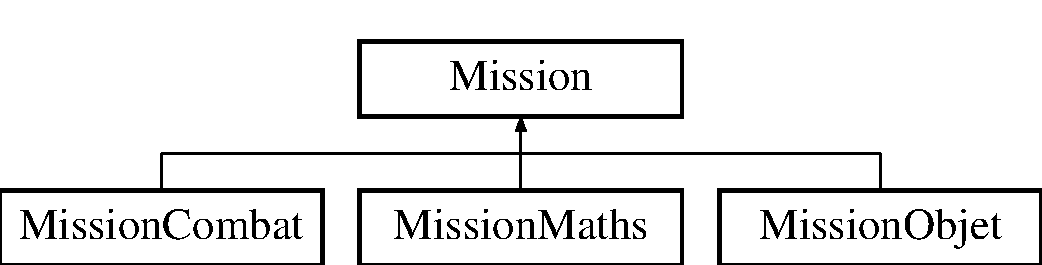
\includegraphics[height=2.000000cm]{class_mission}
\end{center}
\end{figure}
\subsection*{Public Member Functions}
\begin{DoxyCompactItemize}
\item 
\hyperlink{class_mission_a7623e26167975876e1a7f483eed38d33}{Mission} (int acc\-Intel, int acc\-Force, int acc\-Age, int acc\-Energie, string nom, string dialogue\-R, string dialogue\-E)
\begin{DoxyCompactList}\small\item\em Constructeur de la classe mission. \end{DoxyCompactList}\item 
\hyperlink{class_mission_aa5a6ff4fc779338ab01b8f6dd470f4df}{Mission} ()
\begin{DoxyCompactList}\small\item\em Constructeur par défaut. \end{DoxyCompactList}\item 
\hyperlink{class_mission_ad1a61b34162393ac42be5955d9772921}{$\sim$\-Mission} ()
\begin{DoxyCompactList}\small\item\em Destructeur par défaut. \end{DoxyCompactList}\item 
void \hyperlink{class_mission_a8fb06ed6f8b7bf29b75729548c18c5e9}{set\-Access\-Intel} (int new\-\_\-var)
\begin{DoxyCompactList}\small\item\em stock la valeur de la variable new\-\_\-var dans la variable access\-Intel. \end{DoxyCompactList}\item 
int \hyperlink{class_mission_ab3ed2d8bde3f15489406775cec6ca3ae}{get\-Access\-Intel} ()
\begin{DoxyCompactList}\small\item\em Accède à la variable access\-Intel. \end{DoxyCompactList}\item 
void \hyperlink{class_mission_a23c1490b294d170c675279ee9296f1f2}{set\-Access\-Force} (int new\-\_\-var)
\begin{DoxyCompactList}\small\item\em stock la valeur de la variable new\-\_\-var dans la variable access\-Force. \end{DoxyCompactList}\item 
int \hyperlink{class_mission_ae443e12738d9e3c52f27f3630df68bbf}{get\-Access\-Force} ()
\begin{DoxyCompactList}\small\item\em Accède à la variable access\-Force. \end{DoxyCompactList}\item 
void \hyperlink{class_mission_aac3bc744de87abea4e87db51616dfec5}{set\-Access\-Age} (int new\-\_\-var)
\begin{DoxyCompactList}\small\item\em stock la valeur de la variable new\-\_\-var dans la variable access\-Age. \end{DoxyCompactList}\item 
int \hyperlink{class_mission_a3ce0c4da70204a7bd84f9acb6306e43e}{get\-Access\-Age} ()
\begin{DoxyCompactList}\small\item\em Accède à la variable access\-Age. \end{DoxyCompactList}\item 
void \hyperlink{class_mission_a5ee38d2b67b7f860fb6a27d486200bec}{set\-Etat\-Mission} (\hyperlink{mission_8hpp_ace9df1e8554ba5a57340fb42cee370f7}{Etat\-Mission} new\-\_\-var)
\begin{DoxyCompactList}\small\item\em stock la valeur de la variable new\-\_\-var dans la variable etat\-Mission. \end{DoxyCompactList}\item 
\hyperlink{mission_8hpp_ace9df1e8554ba5a57340fb42cee370f7}{Etat\-Mission} \hyperlink{class_mission_aa513084d347dc1c4c8a957258c9d3876}{get\-Etat\-Mission} ()
\begin{DoxyCompactList}\small\item\em Accède à la variable etat\-Mission. \end{DoxyCompactList}\item 
void \hyperlink{class_mission_afc0e70a63822f561abf3a7e832f086af}{set\-Texte\-Mission} (string new\-\_\-var)
\begin{DoxyCompactList}\small\item\em stock la valeur de la variable new\-\_\-var dans la variable texte\-Mission. \end{DoxyCompactList}\item 
string \hyperlink{class_mission_ad6b21ef20ff04bad9769f3b50a3b1218}{get\-Texte\-Mission} ()
\begin{DoxyCompactList}\small\item\em Accède à la variable texte\-Mission. \end{DoxyCompactList}\item 
void \hyperlink{class_mission_a3b2a2ce4cd3025d2233ff593cd87cae0}{set\-Access\-Energie} (int var)
\begin{DoxyCompactList}\small\item\em stock la valeur de la variable var dans la variable access\-Energie. \end{DoxyCompactList}\item 
int \hyperlink{class_mission_a1fd4aa1e267e0f722f6bdb8891ec053f}{get\-Access\-Energie} ()
\begin{DoxyCompactList}\small\item\em Accède à la variable access\-Energie. \end{DoxyCompactList}\item 
string \hyperlink{class_mission_adedaca4409d2abe41a36c04921440b86}{get\-Dialogue\-Reussite} ()
\begin{DoxyCompactList}\small\item\em Accède à la variable dialogue\-Reussite. \end{DoxyCompactList}\item 
void \hyperlink{class_mission_a168753922a0eaf4fc7ed0a311ac70b46}{set\-Dialogue\-Reussite} (string \hyperlink{class_mission_a75d8fc66d0ed01f1f1192e03528a2612}{dialogue\-Reussite})
\begin{DoxyCompactList}\small\item\em stock la valeur de la variable dialogue\-Reussite dans la variable dialogue\-Reussite. \end{DoxyCompactList}\item 
string \hyperlink{class_mission_af9a813bba373bcac25b42e22c8440c1c}{get\-Dialogue\-Echec} ()
\begin{DoxyCompactList}\small\item\em Accède à la variable dialogue\-Echec. \end{DoxyCompactList}\item 
virtual string \hyperlink{class_mission_ad4375f925eda8637d6346ef468747f44}{executer\-Mission} (\hyperlink{class_jeu}{Jeu} jeu, \hyperlink{class_heros}{Heros} $\ast$heros, \hyperlink{class_p_n_j}{P\-N\-J} $\ast$pnj)
\begin{DoxyCompactList}\small\item\em Exécute une mission. C'est une méthode virtuelle qui va être redéfinie dans chacune des classes filles de \hyperlink{class_mission}{Mission}. \end{DoxyCompactList}\end{DoxyCompactItemize}
\subsection*{Protected Attributes}
\begin{DoxyCompactItemize}
\item 
int \hyperlink{class_mission_af93302ac38548302411994e4cbf9b850}{access\-Intel}
\begin{DoxyCompactList}\small\item\em La valeur nécessaire d'intelligence pour accéder à une mission. \end{DoxyCompactList}\item 
int \hyperlink{class_mission_a58a62ea21f7c074d87e8592a009dec49}{access\-Force}
\begin{DoxyCompactList}\small\item\em La valeur nécessaire de la force pour accéder à une mission. \end{DoxyCompactList}\item 
int \hyperlink{class_mission_a78226357c57649c261115d34598f9a8e}{access\-Age}
\begin{DoxyCompactList}\small\item\em La valeur nécessaire d'âge pour accéder à une mission. \end{DoxyCompactList}\item 
int \hyperlink{class_mission_ae767714f7433f66f519468bc1913a5ef}{access\-Energie}
\begin{DoxyCompactList}\small\item\em La valeur nécessaire d'énergie pour accéder à une mission. \end{DoxyCompactList}\item 
\hyperlink{mission_8hpp_ace9df1e8554ba5a57340fb42cee370f7}{Etat\-Mission} \hyperlink{class_mission_a7a3a8c801854fdbc1ddfb73d187e5b2e}{etat\-Mission}
\begin{DoxyCompactList}\small\item\em L'état de chaque mission pour savoir si la mission est pas\-Entamee, en\-Cours ou achevée. \end{DoxyCompactList}\item 
string \hyperlink{class_mission_ac289a213c14ea87ba5740be349c23419}{texte\-Mission}
\begin{DoxyCompactList}\small\item\em Le texte envoyé à l'utilisateur afin qu'il fasse son choix. \end{DoxyCompactList}\item 
string \hyperlink{class_mission_a75d8fc66d0ed01f1f1192e03528a2612}{dialogue\-Reussite}
\begin{DoxyCompactList}\small\item\em Un texte renvoyé à l'utilisateur quand celui-\/ci réussit la mission. \end{DoxyCompactList}\item 
string \hyperlink{class_mission_aeb543b4e12125834e6b8901820db243b}{dialogue\-Echec}
\begin{DoxyCompactList}\small\item\em Un texte renvoyé à l'utilisateur quand celui-\/ci échoue la mission. \end{DoxyCompactList}\end{DoxyCompactItemize}
\subsection*{Static Protected Attributes}
\begin{DoxyCompactItemize}
\item 
static int \hyperlink{class_mission_af6589a43033e50899832cc63939ecb23}{compteur\-Mission} = 1
\begin{DoxyCompactList}\small\item\em Le compteur de la mission. \end{DoxyCompactList}\end{DoxyCompactItemize}


\subsection{Detailed Description}
Classe représentant les missions. 

\subsection{Constructor \& Destructor Documentation}
\hypertarget{class_mission_a7623e26167975876e1a7f483eed38d33}{\index{Mission@{Mission}!Mission@{Mission}}
\index{Mission@{Mission}!Mission@{Mission}}
\subsubsection[{Mission}]{\setlength{\rightskip}{0pt plus 5cm}Mission\-::\-Mission (
\begin{DoxyParamCaption}
\item[{int}]{acc\-Intel, }
\item[{int}]{acc\-Force, }
\item[{int}]{acc\-Age, }
\item[{int}]{acc\-Energie, }
\item[{string}]{nom, }
\item[{string}]{dialogue\-R, }
\item[{string}]{dialogue\-E}
\end{DoxyParamCaption}
)}}\label{class_mission_a7623e26167975876e1a7f483eed38d33}


Constructeur de la classe mission. 


\begin{DoxyParams}{Parameters}
{\em acc\-Intel} & La valeur nécessaire d'intelligence pour accéder à une mission. \\
\hline
{\em acc\-Force} & La valeur nécessaire de la force pour accéder à une mission. \\
\hline
{\em acc\-Age} & La valeur nécessaire d'âge pour accéder à une mission. \\
\hline
{\em access\-Energie} & La valeur nécessaire d'énergie pour accéder à une mission. \\
\hline
{\em nom} & le nom de la mission. \\
\hline
{\em dialogue\-R} & Le dialogue en cas de réussite. \\
\hline
{\em dialogue\-E} & Le dialogue en cas d'échec. \\
\hline
\end{DoxyParams}

\begin{DoxyCode}
14                                                                                                            
                 \{
15     \hyperlink{class_mission_af93302ac38548302411994e4cbf9b850}{accessIntel} = accIntel;
16     \hyperlink{class_mission_a58a62ea21f7c074d87e8592a009dec49}{accessForce} = accForce;
17     \hyperlink{class_mission_a78226357c57649c261115d34598f9a8e}{accessAge} = accAge;
18     \hyperlink{class_mission_ac289a213c14ea87ba5740be349c23419}{texteMission} = nom;
19     \hyperlink{class_mission_ae767714f7433f66f519468bc1913a5ef}{accessEnergie} = accEnergie;
20     \hyperlink{class_mission_a7a3a8c801854fdbc1ddfb73d187e5b2e}{etatMission} = \hyperlink{mission_8hpp_ace9df1e8554ba5a57340fb42cee370f7a008dce2c823a7fc5afc3b4233e8da8d9}{pasEntamee};
21     \hyperlink{class_mission_a75d8fc66d0ed01f1f1192e03528a2612}{dialogueReussite} = dialogueR;
22     \hyperlink{class_mission_aeb543b4e12125834e6b8901820db243b}{dialogueEchec} = dialogueE;
23 
24 \}
\end{DoxyCode}
\hypertarget{class_mission_aa5a6ff4fc779338ab01b8f6dd470f4df}{\index{Mission@{Mission}!Mission@{Mission}}
\index{Mission@{Mission}!Mission@{Mission}}
\subsubsection[{Mission}]{\setlength{\rightskip}{0pt plus 5cm}Mission\-::\-Mission (
\begin{DoxyParamCaption}
{}
\end{DoxyParamCaption}
)}}\label{class_mission_aa5a6ff4fc779338ab01b8f6dd470f4df}


Constructeur par défaut. 


\begin{DoxyCode}
27 \{\};
\end{DoxyCode}
\hypertarget{class_mission_ad1a61b34162393ac42be5955d9772921}{\index{Mission@{Mission}!$\sim$\-Mission@{$\sim$\-Mission}}
\index{$\sim$\-Mission@{$\sim$\-Mission}!Mission@{Mission}}
\subsubsection[{$\sim$\-Mission}]{\setlength{\rightskip}{0pt plus 5cm}Mission\-::$\sim$\-Mission (
\begin{DoxyParamCaption}
{}
\end{DoxyParamCaption}
)}}\label{class_mission_ad1a61b34162393ac42be5955d9772921}


Destructeur par défaut. 


\begin{DoxyCode}
29 \{\};
\end{DoxyCode}


\subsection{Member Function Documentation}
\hypertarget{class_mission_ad4375f925eda8637d6346ef468747f44}{\index{Mission@{Mission}!executer\-Mission@{executer\-Mission}}
\index{executer\-Mission@{executer\-Mission}!Mission@{Mission}}
\subsubsection[{executer\-Mission}]{\setlength{\rightskip}{0pt plus 5cm}string Mission\-::executer\-Mission (
\begin{DoxyParamCaption}
\item[{{\bf Jeu}}]{jeu, }
\item[{{\bf Heros} $\ast$}]{heros, }
\item[{{\bf P\-N\-J} $\ast$}]{pnj}
\end{DoxyParamCaption}
)\hspace{0.3cm}{\ttfamily [virtual]}}}\label{class_mission_ad4375f925eda8637d6346ef468747f44}


Exécute une mission. C'est une méthode virtuelle qui va être redéfinie dans chacune des classes filles de \hyperlink{class_mission}{Mission}. 


\begin{DoxyParams}{Parameters}
{\em jeu} & Une instance de la classe \hyperlink{class_jeu}{Jeu}. \\
\hline
{\em heros} & Un pointeur sur la classe \hyperlink{class_heros}{Heros}. \\
\hline
{\em pnj} & Un pointeur sur la classe \hyperlink{class_p_n_j}{P\-N\-J}. \\
\hline
\end{DoxyParams}
\begin{DoxyReturn}{Returns}
erreur si la mission n'a pas été exécutée. 
\end{DoxyReturn}


Reimplemented in \hyperlink{class_mission_maths_aec614bc24cbe313c5ce6d5d76119a041}{Mission\-Maths}, \hyperlink{class_mission_combat_a66b242eaa5cd9b788e9e26502d885fa7}{Mission\-Combat}, and \hyperlink{class_mission_objet_a49547f2e562b288a9abd640641964f78}{Mission\-Objet}.


\begin{DoxyCode}
94                                                                 \{
95       \textcolor{keywordflow}{return} \textcolor{stringliteral}{"erreur"};
96   \}
\end{DoxyCode}
\hypertarget{class_mission_a3ce0c4da70204a7bd84f9acb6306e43e}{\index{Mission@{Mission}!get\-Access\-Age@{get\-Access\-Age}}
\index{get\-Access\-Age@{get\-Access\-Age}!Mission@{Mission}}
\subsubsection[{get\-Access\-Age}]{\setlength{\rightskip}{0pt plus 5cm}int Mission\-::get\-Access\-Age (
\begin{DoxyParamCaption}
{}
\end{DoxyParamCaption}
)}}\label{class_mission_a3ce0c4da70204a7bd84f9acb6306e43e}


Accède à la variable access\-Age. 

\begin{DoxyReturn}{Returns}
la valeur de l'âge nécessaire pour accèder à une mission. 
\end{DoxyReturn}

\begin{DoxyCode}
53                                  \{
54     \textcolor{keywordflow}{return} \hyperlink{class_mission_a78226357c57649c261115d34598f9a8e}{accessAge};
55   \}
\end{DoxyCode}
\hypertarget{class_mission_a1fd4aa1e267e0f722f6bdb8891ec053f}{\index{Mission@{Mission}!get\-Access\-Energie@{get\-Access\-Energie}}
\index{get\-Access\-Energie@{get\-Access\-Energie}!Mission@{Mission}}
\subsubsection[{get\-Access\-Energie}]{\setlength{\rightskip}{0pt plus 5cm}int Mission\-::get\-Access\-Energie (
\begin{DoxyParamCaption}
{}
\end{DoxyParamCaption}
)}}\label{class_mission_a1fd4aa1e267e0f722f6bdb8891ec053f}


Accède à la variable access\-Energie. 

\begin{DoxyReturn}{Returns}
la valeur de l'énergie nécessaire pour accèder à une mission. 
\end{DoxyReturn}

\begin{DoxyCode}
90                                 \{
91     \textcolor{keywordflow}{return} \hyperlink{class_mission_ae767714f7433f66f519468bc1913a5ef}{accessEnergie};
92   \}
\end{DoxyCode}
\hypertarget{class_mission_ae443e12738d9e3c52f27f3630df68bbf}{\index{Mission@{Mission}!get\-Access\-Force@{get\-Access\-Force}}
\index{get\-Access\-Force@{get\-Access\-Force}!Mission@{Mission}}
\subsubsection[{get\-Access\-Force}]{\setlength{\rightskip}{0pt plus 5cm}int Mission\-::get\-Access\-Force (
\begin{DoxyParamCaption}
{}
\end{DoxyParamCaption}
)}}\label{class_mission_ae443e12738d9e3c52f27f3630df68bbf}


Accède à la variable access\-Force. 

\begin{DoxyReturn}{Returns}
la valeur de la force nécessaire pour accèder à une mission. 
\end{DoxyReturn}

\begin{DoxyCode}
45                                    \{
46     \textcolor{keywordflow}{return} \hyperlink{class_mission_a58a62ea21f7c074d87e8592a009dec49}{accessForce};
47   \}
\end{DoxyCode}
\hypertarget{class_mission_ab3ed2d8bde3f15489406775cec6ca3ae}{\index{Mission@{Mission}!get\-Access\-Intel@{get\-Access\-Intel}}
\index{get\-Access\-Intel@{get\-Access\-Intel}!Mission@{Mission}}
\subsubsection[{get\-Access\-Intel}]{\setlength{\rightskip}{0pt plus 5cm}int Mission\-::get\-Access\-Intel (
\begin{DoxyParamCaption}
{}
\end{DoxyParamCaption}
)}}\label{class_mission_ab3ed2d8bde3f15489406775cec6ca3ae}


Accède à la variable access\-Intel. 

\begin{DoxyReturn}{Returns}
la valeur de l'intelligence nécessaire pour accèder à une mission. 
\end{DoxyReturn}

\begin{DoxyCode}
37                                    \{
38     \textcolor{keywordflow}{return} \hyperlink{class_mission_af93302ac38548302411994e4cbf9b850}{accessIntel};
39   \}
\end{DoxyCode}
\hypertarget{class_mission_af9a813bba373bcac25b42e22c8440c1c}{\index{Mission@{Mission}!get\-Dialogue\-Echec@{get\-Dialogue\-Echec}}
\index{get\-Dialogue\-Echec@{get\-Dialogue\-Echec}!Mission@{Mission}}
\subsubsection[{get\-Dialogue\-Echec}]{\setlength{\rightskip}{0pt plus 5cm}string Mission\-::get\-Dialogue\-Echec (
\begin{DoxyParamCaption}
{}
\end{DoxyParamCaption}
)}}\label{class_mission_af9a813bba373bcac25b42e22c8440c1c}


Accède à la variable dialogue\-Echec. 

\begin{DoxyReturn}{Returns}
Un texte afin d'indiquer si la mission a été échouée. 
\end{DoxyReturn}

\begin{DoxyCode}
82                                     \{
83         \textcolor{keywordflow}{return} \hyperlink{class_mission_aeb543b4e12125834e6b8901820db243b}{dialogueEchec};
84     \}
\end{DoxyCode}
\hypertarget{class_mission_adedaca4409d2abe41a36c04921440b86}{\index{Mission@{Mission}!get\-Dialogue\-Reussite@{get\-Dialogue\-Reussite}}
\index{get\-Dialogue\-Reussite@{get\-Dialogue\-Reussite}!Mission@{Mission}}
\subsubsection[{get\-Dialogue\-Reussite}]{\setlength{\rightskip}{0pt plus 5cm}string Mission\-::get\-Dialogue\-Reussite (
\begin{DoxyParamCaption}
{}
\end{DoxyParamCaption}
)}}\label{class_mission_adedaca4409d2abe41a36c04921440b86}


Accède à la variable dialogue\-Reussite. 

\begin{DoxyReturn}{Returns}
Un texte afin d'indiquer si la mission a été réussie. 
\end{DoxyReturn}

\begin{DoxyCode}
74                                          \{
75         \textcolor{keywordflow}{return} \hyperlink{class_mission_a75d8fc66d0ed01f1f1192e03528a2612}{dialogueReussite};
76     \}
\end{DoxyCode}
\hypertarget{class_mission_aa513084d347dc1c4c8a957258c9d3876}{\index{Mission@{Mission}!get\-Etat\-Mission@{get\-Etat\-Mission}}
\index{get\-Etat\-Mission@{get\-Etat\-Mission}!Mission@{Mission}}
\subsubsection[{get\-Etat\-Mission}]{\setlength{\rightskip}{0pt plus 5cm}{\bf Etat\-Mission} Mission\-::get\-Etat\-Mission (
\begin{DoxyParamCaption}
{}
\end{DoxyParamCaption}
)}}\label{class_mission_aa513084d347dc1c4c8a957258c9d3876}


Accède à la variable etat\-Mission. 

\begin{DoxyReturn}{Returns}
L'état de la mission par exemple pas\-Entame, en\-Cours ou achevee. 
\end{DoxyReturn}

\begin{DoxyCode}
62                                            \{
63     \textcolor{keywordflow}{return} \hyperlink{class_mission_a7a3a8c801854fdbc1ddfb73d187e5b2e}{etatMission};
64   \}
\end{DoxyCode}
\hypertarget{class_mission_ad6b21ef20ff04bad9769f3b50a3b1218}{\index{Mission@{Mission}!get\-Texte\-Mission@{get\-Texte\-Mission}}
\index{get\-Texte\-Mission@{get\-Texte\-Mission}!Mission@{Mission}}
\subsubsection[{get\-Texte\-Mission}]{\setlength{\rightskip}{0pt plus 5cm}string Mission\-::get\-Texte\-Mission (
\begin{DoxyParamCaption}
{}
\end{DoxyParamCaption}
)}}\label{class_mission_ad6b21ef20ff04bad9769f3b50a3b1218}


Accède à la variable texte\-Mission. 

\begin{DoxyReturn}{Returns}
Le texte permettant de choisir une mission par l'utilisateur . 
\end{DoxyReturn}

\begin{DoxyCode}
70                                        \{
71     \textcolor{keywordflow}{return} \hyperlink{class_mission_ac289a213c14ea87ba5740be349c23419}{texteMission};
72   \}
\end{DoxyCode}
\hypertarget{class_mission_aac3bc744de87abea4e87db51616dfec5}{\index{Mission@{Mission}!set\-Access\-Age@{set\-Access\-Age}}
\index{set\-Access\-Age@{set\-Access\-Age}!Mission@{Mission}}
\subsubsection[{set\-Access\-Age}]{\setlength{\rightskip}{0pt plus 5cm}void Mission\-::set\-Access\-Age (
\begin{DoxyParamCaption}
\item[{int}]{new\-\_\-var}
\end{DoxyParamCaption}
)}}\label{class_mission_aac3bc744de87abea4e87db51616dfec5}


stock la valeur de la variable new\-\_\-var dans la variable access\-Age. 


\begin{DoxyCode}
49                                             \{
50       \hyperlink{class_mission_a78226357c57649c261115d34598f9a8e}{accessAge} = new\_var;
51   \}
\end{DoxyCode}
\hypertarget{class_mission_a3b2a2ce4cd3025d2233ff593cd87cae0}{\index{Mission@{Mission}!set\-Access\-Energie@{set\-Access\-Energie}}
\index{set\-Access\-Energie@{set\-Access\-Energie}!Mission@{Mission}}
\subsubsection[{set\-Access\-Energie}]{\setlength{\rightskip}{0pt plus 5cm}void Mission\-::set\-Access\-Energie (
\begin{DoxyParamCaption}
\item[{int}]{var}
\end{DoxyParamCaption}
)}}\label{class_mission_a3b2a2ce4cd3025d2233ff593cd87cae0}


stock la valeur de la variable var dans la variable access\-Energie. 


\begin{DoxyCode}
86                                         \{
87     \hyperlink{class_mission_ae767714f7433f66f519468bc1913a5ef}{accessEnergie} = var;
88   \}
\end{DoxyCode}
\hypertarget{class_mission_a23c1490b294d170c675279ee9296f1f2}{\index{Mission@{Mission}!set\-Access\-Force@{set\-Access\-Force}}
\index{set\-Access\-Force@{set\-Access\-Force}!Mission@{Mission}}
\subsubsection[{set\-Access\-Force}]{\setlength{\rightskip}{0pt plus 5cm}void Mission\-::set\-Access\-Force (
\begin{DoxyParamCaption}
\item[{int}]{new\-\_\-var}
\end{DoxyParamCaption}
)}}\label{class_mission_a23c1490b294d170c675279ee9296f1f2}


stock la valeur de la variable new\-\_\-var dans la variable access\-Force. 


\begin{DoxyCode}
41                                                \{
42       \hyperlink{class_mission_a58a62ea21f7c074d87e8592a009dec49}{accessForce} = new\_var;
43   \}
\end{DoxyCode}
\hypertarget{class_mission_a8fb06ed6f8b7bf29b75729548c18c5e9}{\index{Mission@{Mission}!set\-Access\-Intel@{set\-Access\-Intel}}
\index{set\-Access\-Intel@{set\-Access\-Intel}!Mission@{Mission}}
\subsubsection[{set\-Access\-Intel}]{\setlength{\rightskip}{0pt plus 5cm}void Mission\-::set\-Access\-Intel (
\begin{DoxyParamCaption}
\item[{int}]{new\-\_\-var}
\end{DoxyParamCaption}
)}}\label{class_mission_a8fb06ed6f8b7bf29b75729548c18c5e9}


stock la valeur de la variable new\-\_\-var dans la variable access\-Intel. 


\begin{DoxyCode}
33                                               \{
34       \hyperlink{class_mission_af93302ac38548302411994e4cbf9b850}{accessIntel} = new\_var;
35   \}
\end{DoxyCode}
\hypertarget{class_mission_a168753922a0eaf4fc7ed0a311ac70b46}{\index{Mission@{Mission}!set\-Dialogue\-Reussite@{set\-Dialogue\-Reussite}}
\index{set\-Dialogue\-Reussite@{set\-Dialogue\-Reussite}!Mission@{Mission}}
\subsubsection[{set\-Dialogue\-Reussite}]{\setlength{\rightskip}{0pt plus 5cm}void Mission\-::set\-Dialogue\-Reussite (
\begin{DoxyParamCaption}
\item[{string}]{dialogue\-Reussite}
\end{DoxyParamCaption}
)}}\label{class_mission_a168753922a0eaf4fc7ed0a311ac70b46}


stock la valeur de la variable dialogue\-Reussite dans la variable dialogue\-Reussite. 


\begin{DoxyCode}
78                                                              \{
79         this->\hyperlink{class_mission_a75d8fc66d0ed01f1f1192e03528a2612}{dialogueReussite} = \hyperlink{class_mission_a75d8fc66d0ed01f1f1192e03528a2612}{dialogueReussite};
80     \}
\end{DoxyCode}
\hypertarget{class_mission_a5ee38d2b67b7f860fb6a27d486200bec}{\index{Mission@{Mission}!set\-Etat\-Mission@{set\-Etat\-Mission}}
\index{set\-Etat\-Mission@{set\-Etat\-Mission}!Mission@{Mission}}
\subsubsection[{set\-Etat\-Mission}]{\setlength{\rightskip}{0pt plus 5cm}void Mission\-::set\-Etat\-Mission (
\begin{DoxyParamCaption}
\item[{{\bf Etat\-Mission}}]{new\-\_\-var}
\end{DoxyParamCaption}
)}}\label{class_mission_a5ee38d2b67b7f860fb6a27d486200bec}


stock la valeur de la variable new\-\_\-var dans la variable etat\-Mission. 


\begin{DoxyCode}
57                                                        \{
58       \hyperlink{class_mission_a7a3a8c801854fdbc1ddfb73d187e5b2e}{etatMission} = new\_var;
59   \}
\end{DoxyCode}
\hypertarget{class_mission_afc0e70a63822f561abf3a7e832f086af}{\index{Mission@{Mission}!set\-Texte\-Mission@{set\-Texte\-Mission}}
\index{set\-Texte\-Mission@{set\-Texte\-Mission}!Mission@{Mission}}
\subsubsection[{set\-Texte\-Mission}]{\setlength{\rightskip}{0pt plus 5cm}void Mission\-::set\-Texte\-Mission (
\begin{DoxyParamCaption}
\item[{string}]{new\-\_\-var}
\end{DoxyParamCaption}
)}}\label{class_mission_afc0e70a63822f561abf3a7e832f086af}


stock la valeur de la variable new\-\_\-var dans la variable texte\-Mission. 


\begin{DoxyCode}
66                                                    \{
67       \hyperlink{class_mission_ac289a213c14ea87ba5740be349c23419}{texteMission} = new\_var;
68   \}
\end{DoxyCode}


\subsection{Member Data Documentation}
\hypertarget{class_mission_a78226357c57649c261115d34598f9a8e}{\index{Mission@{Mission}!access\-Age@{access\-Age}}
\index{access\-Age@{access\-Age}!Mission@{Mission}}
\subsubsection[{access\-Age}]{\setlength{\rightskip}{0pt plus 5cm}int Mission\-::access\-Age\hspace{0.3cm}{\ttfamily [protected]}}}\label{class_mission_a78226357c57649c261115d34598f9a8e}


La valeur nécessaire d'âge pour accéder à une mission. 

\hypertarget{class_mission_ae767714f7433f66f519468bc1913a5ef}{\index{Mission@{Mission}!access\-Energie@{access\-Energie}}
\index{access\-Energie@{access\-Energie}!Mission@{Mission}}
\subsubsection[{access\-Energie}]{\setlength{\rightskip}{0pt plus 5cm}int Mission\-::access\-Energie\hspace{0.3cm}{\ttfamily [protected]}}}\label{class_mission_ae767714f7433f66f519468bc1913a5ef}


La valeur nécessaire d'énergie pour accéder à une mission. 

\hypertarget{class_mission_a58a62ea21f7c074d87e8592a009dec49}{\index{Mission@{Mission}!access\-Force@{access\-Force}}
\index{access\-Force@{access\-Force}!Mission@{Mission}}
\subsubsection[{access\-Force}]{\setlength{\rightskip}{0pt plus 5cm}int Mission\-::access\-Force\hspace{0.3cm}{\ttfamily [protected]}}}\label{class_mission_a58a62ea21f7c074d87e8592a009dec49}


La valeur nécessaire de la force pour accéder à une mission. 

\hypertarget{class_mission_af93302ac38548302411994e4cbf9b850}{\index{Mission@{Mission}!access\-Intel@{access\-Intel}}
\index{access\-Intel@{access\-Intel}!Mission@{Mission}}
\subsubsection[{access\-Intel}]{\setlength{\rightskip}{0pt plus 5cm}int Mission\-::access\-Intel\hspace{0.3cm}{\ttfamily [protected]}}}\label{class_mission_af93302ac38548302411994e4cbf9b850}


La valeur nécessaire d'intelligence pour accéder à une mission. 

\hypertarget{class_mission_af6589a43033e50899832cc63939ecb23}{\index{Mission@{Mission}!compteur\-Mission@{compteur\-Mission}}
\index{compteur\-Mission@{compteur\-Mission}!Mission@{Mission}}
\subsubsection[{compteur\-Mission}]{\setlength{\rightskip}{0pt plus 5cm}int Mission\-::compteur\-Mission = 1\hspace{0.3cm}{\ttfamily [static]}, {\ttfamily [protected]}}}\label{class_mission_af6589a43033e50899832cc63939ecb23}


Le compteur de la mission. 

\hypertarget{class_mission_aeb543b4e12125834e6b8901820db243b}{\index{Mission@{Mission}!dialogue\-Echec@{dialogue\-Echec}}
\index{dialogue\-Echec@{dialogue\-Echec}!Mission@{Mission}}
\subsubsection[{dialogue\-Echec}]{\setlength{\rightskip}{0pt plus 5cm}string Mission\-::dialogue\-Echec\hspace{0.3cm}{\ttfamily [protected]}}}\label{class_mission_aeb543b4e12125834e6b8901820db243b}


Un texte renvoyé à l'utilisateur quand celui-\/ci échoue la mission. 

\hypertarget{class_mission_a75d8fc66d0ed01f1f1192e03528a2612}{\index{Mission@{Mission}!dialogue\-Reussite@{dialogue\-Reussite}}
\index{dialogue\-Reussite@{dialogue\-Reussite}!Mission@{Mission}}
\subsubsection[{dialogue\-Reussite}]{\setlength{\rightskip}{0pt plus 5cm}string Mission\-::dialogue\-Reussite\hspace{0.3cm}{\ttfamily [protected]}}}\label{class_mission_a75d8fc66d0ed01f1f1192e03528a2612}


Un texte renvoyé à l'utilisateur quand celui-\/ci réussit la mission. 

\hypertarget{class_mission_a7a3a8c801854fdbc1ddfb73d187e5b2e}{\index{Mission@{Mission}!etat\-Mission@{etat\-Mission}}
\index{etat\-Mission@{etat\-Mission}!Mission@{Mission}}
\subsubsection[{etat\-Mission}]{\setlength{\rightskip}{0pt plus 5cm}{\bf Etat\-Mission} Mission\-::etat\-Mission\hspace{0.3cm}{\ttfamily [protected]}}}\label{class_mission_a7a3a8c801854fdbc1ddfb73d187e5b2e}


L'état de chaque mission pour savoir si la mission est pas\-Entamee, en\-Cours ou achevée. 

\hypertarget{class_mission_ac289a213c14ea87ba5740be349c23419}{\index{Mission@{Mission}!texte\-Mission@{texte\-Mission}}
\index{texte\-Mission@{texte\-Mission}!Mission@{Mission}}
\subsubsection[{texte\-Mission}]{\setlength{\rightskip}{0pt plus 5cm}string Mission\-::texte\-Mission\hspace{0.3cm}{\ttfamily [protected]}}}\label{class_mission_ac289a213c14ea87ba5740be349c23419}


Le texte envoyé à l'utilisateur afin qu'il fasse son choix. 



The documentation for this class was generated from the following files\-:\begin{DoxyCompactItemize}
\item 
/nfs/usersgm/\-G\-M26/neljibbawe/\-Bureau/\-Projet\-C\-P\-P\-A\-Rendre/\-C\-P\-P R\-P\-G/\-R\-P\-G/\hyperlink{mission_8hpp}{mission.\-hpp}\item 
/nfs/usersgm/\-G\-M26/neljibbawe/\-Bureau/\-Projet\-C\-P\-P\-A\-Rendre/\-C\-P\-P R\-P\-G/\-R\-P\-G/\hyperlink{mission_8cpp}{mission.\-cpp}\end{DoxyCompactItemize}

\hypertarget{class_mission_combat}{\section{Mission\-Combat Class Reference}
\label{class_mission_combat}\index{Mission\-Combat@{Mission\-Combat}}
}


Classe représentant les missions de type combat.  




{\ttfamily \#include $<$missioncombat.\-hpp$>$}

Inheritance diagram for Mission\-Combat\-:\begin{figure}[H]
\begin{center}
\leavevmode
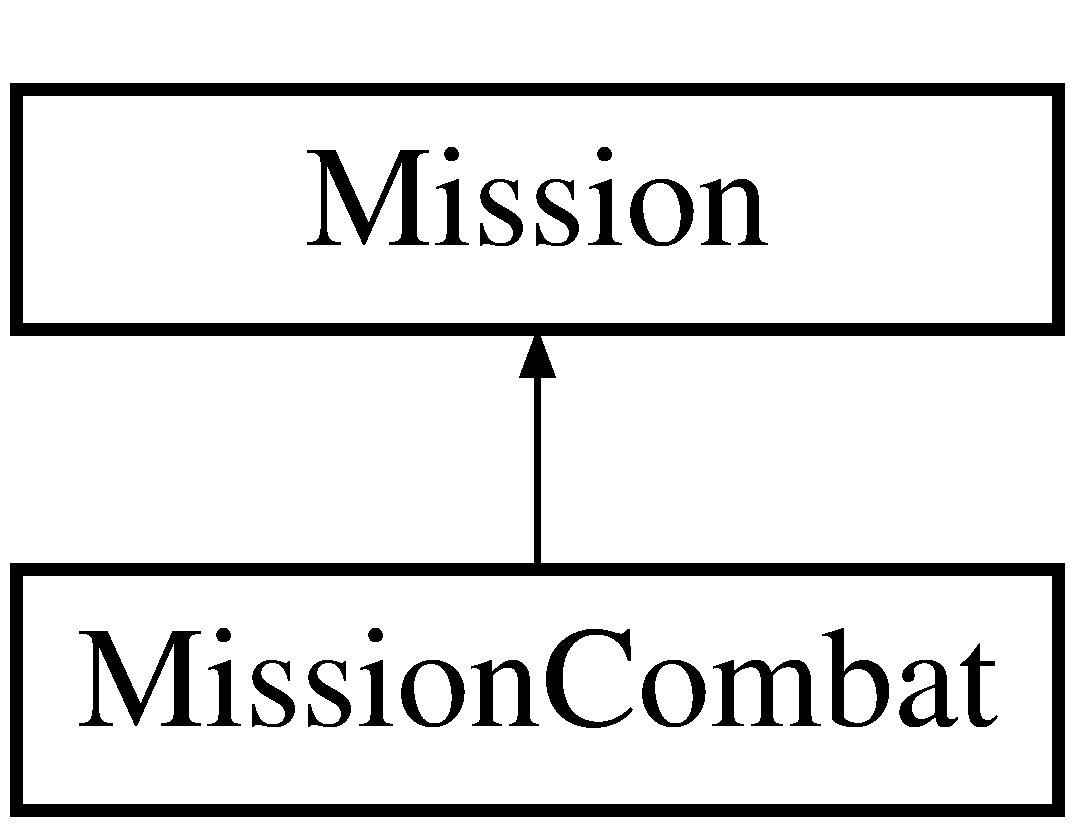
\includegraphics[height=2.000000cm]{class_mission_combat}
\end{center}
\end{figure}
\subsection*{Public Member Functions}
\begin{DoxyCompactItemize}
\item 
\hyperlink{class_mission_combat_a16d2c93a4366d48fb6ea6339388c76c4}{Mission\-Combat} ()
\begin{DoxyCompactList}\small\item\em Constructeur par défaut. \end{DoxyCompactList}\item 
\hyperlink{class_mission_combat_a7599e8cb49f2e49b8a54cfbf836c2f42}{Mission\-Combat} (int acc\-Intel, int acc\-Force, int acc\-Age, int acc\-Energie, string nom, int rec\-Force, int rec\-Cash, string dialogue\-R, string dialogue\-E)
\begin{DoxyCompactList}\small\item\em Constructeur de la classe mission combat . \end{DoxyCompactList}\item 
void \hyperlink{class_mission_combat_ad838e9ec99671e81fe9b0edb18b81f02}{set\-Recomp\-Force} (int new\-\_\-var)
\begin{DoxyCompactList}\small\item\em stock la valeur de la variable new\-\_\-var dans la variable recomp\-Force. \end{DoxyCompactList}\item 
int \hyperlink{class_mission_combat_a47460faf8b07a407771f11249fbe26d1}{get\-Recomp\-Force} ()
\begin{DoxyCompactList}\small\item\em Accède à la variable recomp\-Force. \end{DoxyCompactList}\item 
void \hyperlink{class_mission_combat_a8d9d56b01541e6ec190a029ddb9861e3}{set\-Recomp\-Cash} (int new\-\_\-var)
\begin{DoxyCompactList}\small\item\em stock la valeur de la variable new\-\_\-var dans la variable recomp\-Cash. \end{DoxyCompactList}\item 
int \hyperlink{class_mission_combat_ac8acd44a461561bd13f718c099bdd416}{get\-Recomp\-Cash} ()
\begin{DoxyCompactList}\small\item\em Accède à la variable recomp\-Cash. \end{DoxyCompactList}\item 
bool \hyperlink{class_mission_combat_a983b1a729c2aedf312c4c61029d14294}{test\-Validite} (\hyperlink{class_heros}{Heros} $\ast$heros, \hyperlink{class_p_n_j}{P\-N\-J} $\ast$pnj)
\begin{DoxyCompactList}\small\item\em Teste la validité de la mission combat. \end{DoxyCompactList}\item 
\hyperlink{class_personnage}{Personnage} $\ast$ \hyperlink{class_mission_combat_a511ab55d291861d8c000fcba73393f44}{comparer\-Stats} (\hyperlink{class_heros}{Heros} $\ast$hero, \hyperlink{class_p_n_j}{P\-N\-J} $\ast$pnj)
\begin{DoxyCompactList}\small\item\em Compare les statistiques du héros avec celles du \hyperlink{class_p_n_j}{P\-N\-J}. \end{DoxyCompactList}\item 
string \hyperlink{class_mission_combat_a66b242eaa5cd9b788e9e26502d885fa7}{executer\-Mission} (\hyperlink{class_jeu}{Jeu} jeu, \hyperlink{class_heros}{Heros} $\ast$heros, \hyperlink{class_p_n_j}{P\-N\-J} $\ast$pnj)
\begin{DoxyCompactList}\small\item\em Exécute une mission de type combat. \end{DoxyCompactList}\end{DoxyCompactItemize}
\subsection*{Additional Inherited Members}


\subsection{Detailed Description}
Classe représentant les missions de type combat. 

\subsection{Constructor \& Destructor Documentation}
\hypertarget{class_mission_combat_a16d2c93a4366d48fb6ea6339388c76c4}{\index{Mission\-Combat@{Mission\-Combat}!Mission\-Combat@{Mission\-Combat}}
\index{Mission\-Combat@{Mission\-Combat}!MissionCombat@{Mission\-Combat}}
\subsubsection[{Mission\-Combat}]{\setlength{\rightskip}{0pt plus 5cm}Mission\-Combat\-::\-Mission\-Combat (
\begin{DoxyParamCaption}
{}
\end{DoxyParamCaption}
)}}\label{class_mission_combat_a16d2c93a4366d48fb6ea6339388c76c4}


Constructeur par défaut. 


\begin{DoxyCode}
16 \{\}
\end{DoxyCode}
\hypertarget{class_mission_combat_a7599e8cb49f2e49b8a54cfbf836c2f42}{\index{Mission\-Combat@{Mission\-Combat}!Mission\-Combat@{Mission\-Combat}}
\index{Mission\-Combat@{Mission\-Combat}!MissionCombat@{Mission\-Combat}}
\subsubsection[{Mission\-Combat}]{\setlength{\rightskip}{0pt plus 5cm}Mission\-Combat\-::\-Mission\-Combat (
\begin{DoxyParamCaption}
\item[{int}]{acc\-Intel, }
\item[{int}]{acc\-Force, }
\item[{int}]{acc\-Age, }
\item[{int}]{acc\-Energie, }
\item[{string}]{nom, }
\item[{int}]{rec\-Force, }
\item[{int}]{rec\-Cash, }
\item[{string}]{dialogue\-R, }
\item[{string}]{dialogue\-E}
\end{DoxyParamCaption}
)}}\label{class_mission_combat_a7599e8cb49f2e49b8a54cfbf836c2f42}


Constructeur de la classe mission combat . 


\begin{DoxyParams}{Parameters}
{\em acc\-Intel} & La valeur nécessaire d'intelligence pour accéder à une mission. \\
\hline
{\em acc\-Force} & La valeur nécessaire de la force pour accéder à une mission. \\
\hline
{\em acc\-Age} & La valeur nécessaire d'âge pour accéder à une mission. \\
\hline
{\em access\-Energie} & La valeur nécessaire d'énergie pour accéder à une mission. \\
\hline
{\em nom} & le nom de la mission. \\
\hline
{\em rec\-Force} & La valeur de la récompense force que l'héros peut gagner. \\
\hline
{\em rec\-Cash} & La valeur de la récompense cash que l'héros peut gagner \\
\hline
{\em dialogue\-R} & Le dialogue en cas de réussite. \\
\hline
{\em dialogue\-E} & Le dialogue en cas d'échec. \\
\hline
\end{DoxyParams}

\begin{DoxyCode}
17                                                                                                            
                                                      : \hyperlink{class_mission_aa5a6ff4fc779338ab01b8f6dd470f4df}{Mission}(accIntel,accForce,accAge,accEnergie,nom, 
      dialogueR, dialogueE) \{
18     recompForce = recForce;
19     recompCash = recCash;
20     \}
\end{DoxyCode}


\subsection{Member Function Documentation}
\hypertarget{class_mission_combat_a511ab55d291861d8c000fcba73393f44}{\index{Mission\-Combat@{Mission\-Combat}!comparer\-Stats@{comparer\-Stats}}
\index{comparer\-Stats@{comparer\-Stats}!MissionCombat@{Mission\-Combat}}
\subsubsection[{comparer\-Stats}]{\setlength{\rightskip}{0pt plus 5cm}{\bf Personnage} $\ast$ Mission\-Combat\-::comparer\-Stats (
\begin{DoxyParamCaption}
\item[{{\bf Heros} $\ast$}]{hero, }
\item[{{\bf P\-N\-J} $\ast$}]{pnj}
\end{DoxyParamCaption}
)}}\label{class_mission_combat_a511ab55d291861d8c000fcba73393f44}


Compare les statistiques du héros avec celles du \hyperlink{class_p_n_j}{P\-N\-J}. 


\begin{DoxyParams}{Parameters}
{\em heros} & Un paramètre de la classe \hyperlink{class_heros}{Heros}. \\
\hline
{\em pnj} & Un paramètre de la classe \hyperlink{class_p_n_j}{P\-N\-J}. \\
\hline
\end{DoxyParams}
\begin{DoxyReturn}{Returns}
Un personnage qui peut être soit l'héros soit le \hyperlink{class_p_n_j}{P\-N\-J}. 
\end{DoxyReturn}

\begin{DoxyCode}
38                                                                 \{
39     \textcolor{keywordflow}{if}(heros->getForce() > pnj->\hyperlink{class_personnage_a40de0ba95f25eb6f1653b6a4183763ae}{getForce}())
40         \textcolor{keywordflow}{return} heros;
41     \textcolor{keywordflow}{else} \textcolor{keywordflow}{return} pnj;
42   \}
\end{DoxyCode}
\hypertarget{class_mission_combat_a66b242eaa5cd9b788e9e26502d885fa7}{\index{Mission\-Combat@{Mission\-Combat}!executer\-Mission@{executer\-Mission}}
\index{executer\-Mission@{executer\-Mission}!MissionCombat@{Mission\-Combat}}
\subsubsection[{executer\-Mission}]{\setlength{\rightskip}{0pt plus 5cm}string Mission\-Combat\-::executer\-Mission (
\begin{DoxyParamCaption}
\item[{{\bf Jeu}}]{jeu, }
\item[{{\bf Heros} $\ast$}]{heros, }
\item[{{\bf P\-N\-J} $\ast$}]{pnj}
\end{DoxyParamCaption}
)\hspace{0.3cm}{\ttfamily [virtual]}}}\label{class_mission_combat_a66b242eaa5cd9b788e9e26502d885fa7}


Exécute une mission de type combat. 


\begin{DoxyParams}{Parameters}
{\em jeu} & Une instance de la classe \hyperlink{class_jeu}{Jeu}. \\
\hline
{\em heros} & Un pointeur sur la classe \hyperlink{class_heros}{Heros}. \\
\hline
{\em pnj} & Un pointeur sur la classe \hyperlink{class_p_n_j}{P\-N\-J}. \\
\hline
\end{DoxyParams}
\begin{DoxyReturn}{Returns}
Un texte permettant de savoir si le héros a assez de force pour combattre, s'il a gagné ou perdu le combat etc. 
\end{DoxyReturn}


Reimplemented from \hyperlink{class_mission_ad4375f925eda8637d6346ef468747f44}{Mission}.


\begin{DoxyCode}
50                                                                          \{
51 
52       \textcolor{keywordflow}{if}(heros->\hyperlink{class_heros_ae9bbef6d2edcb8b14d9ec3854146a42c}{getEnergie}()<=\hyperlink{class_mission_ae767714f7433f66f519468bc1913a5ef}{accessEnergie})
53           \textcolor{keywordflow}{return} \textcolor{stringliteral}{"Vous n'avez pas assez d'énergie... C'est peut être mieux comme ça remarquez."};
54 
55       \textcolor{keywordflow}{else} \textcolor{keywordflow}{if}(jeu.\hyperlink{class_jeu_a3aa07b1e7a5e5d82479b8bb2a2841635}{demanderBoolUtilisateur}(\textcolor{stringliteral}{"Voulez vous combattre "}+pnj->
      \hyperlink{class_personnage_a519301399a9bee1557858aa50a04a85a}{getNom}()+\textcolor{stringliteral}{" ?"})) \{
56             \hyperlink{class_mission_a5ee38d2b67b7f860fb6a27d486200bec}{setEtatMission}(\hyperlink{mission_8hpp_ace9df1e8554ba5a57340fb42cee370f7aca12092e4757cb029f1b3e1fa95ed277}{enCours});
57             heros->\hyperlink{class_heros_a5d4f5d3d3a4db451923f0609a3e1b53c}{setEnergie}(heros->\hyperlink{class_heros_ae9bbef6d2edcb8b14d9ec3854146a42c}{getEnergie}()-
      \hyperlink{class_mission_ae767714f7433f66f519468bc1913a5ef}{accessEnergie});
58             jeu.\hyperlink{class_jeu_aa09fb40439f16b9665a0d76679f78e4e}{afficherTexte}(\textcolor{stringliteral}{"Vous avez perdu "}+\hyperlink{missioncombat_8cpp_a0d2f37137ee1fd6ff4a0ef803849dd63}{SSTR}(
      \hyperlink{class_mission_ae767714f7433f66f519468bc1913a5ef}{accessEnergie})+\textcolor{stringliteral}{" d'énergie."});
59             jeu.\hyperlink{class_jeu_a52ce4fb6c415b45209db13a589c9d675}{timer}(1, pnj->\hyperlink{class_personnage_a519301399a9bee1557858aa50a04a85a}{getNom}()+\textcolor{stringliteral}{" se retrousse les manches."});
60             jeu.\hyperlink{class_jeu_a52ce4fb6c415b45209db13a589c9d675}{timer}(5, \textcolor{stringliteral}{"Des coups pleuvent dans tous les sens, le combat fait rage..."});
61           \textcolor{keywordflow}{if} (\hyperlink{class_mission_combat_a983b1a729c2aedf312c4c61029d14294}{testValidite}(heros, pnj))\{
62               \hyperlink{class_mission_a5ee38d2b67b7f860fb6a27d486200bec}{setEtatMission}(\hyperlink{mission_8hpp_ace9df1e8554ba5a57340fb42cee370f7a9e765bd835523da043a754ce21905cb5}{achevee});
63               heros->\hyperlink{class_heros_ae87dba7afa03e7fdacfc3a7e82d3a6a3}{setCash}(heros->\hyperlink{class_heros_a77bdee21cb8c8356448bb6669941441c}{getCash}()+recompCash);
64               heros->\hyperlink{class_personnage_a6745d147720906f2c85ddce11981d71f}{setForce}(heros->\hyperlink{class_personnage_a40de0ba95f25eb6f1653b6a4183763ae}{getForce}()+recompForce);
65               \textcolor{keywordflow}{return} pnj->\hyperlink{class_personnage_a519301399a9bee1557858aa50a04a85a}{getNom}()+\textcolor{stringliteral}{" : "}+\hyperlink{class_mission_adedaca4409d2abe41a36c04921440b86}{getDialogueReussite}()+\textcolor{stringliteral}{"\(\backslash\)nVous avez gagné
       le combat, quelle musculature incroyable, je vous croquerai bien...hum. Vous gagnez : "}+
      \hyperlink{missioncombat_8cpp_a0d2f37137ee1fd6ff4a0ef803849dd63}{SSTR}(recompCash)+\textcolor{stringliteral}{" de cash et "}+\hyperlink{missioncombat_8cpp_a0d2f37137ee1fd6ff4a0ef803849dd63}{SSTR}(recompForce)+\textcolor{stringliteral}{" de force"};
66           \}
67           \textcolor{keywordflow}{else} \{
68               \textcolor{keywordflow}{if} (heros->\hyperlink{class_heros_ae9bbef6d2edcb8b14d9ec3854146a42c}{getEnergie}()>heros->\hyperlink{class_personnage_a40de0ba95f25eb6f1653b6a4183763ae}{getForce}()/3)
69             heros->\hyperlink{class_heros_a5d4f5d3d3a4db451923f0609a3e1b53c}{setEnergie}(heros->\hyperlink{class_heros_ae9bbef6d2edcb8b14d9ec3854146a42c}{getEnergie}()-(heros->
      \hyperlink{class_personnage_a40de0ba95f25eb6f1653b6a4183763ae}{getForce}()/3));
70               \textcolor{keywordflow}{else} heros->\hyperlink{class_heros_a5d4f5d3d3a4db451923f0609a3e1b53c}{setEnergie}(0);
71 
72               \textcolor{keywordflow}{if} (heros->\hyperlink{class_heros_a77bdee21cb8c8356448bb6669941441c}{getCash}() > recompCash*2)
73             heros->\hyperlink{class_heros_ae87dba7afa03e7fdacfc3a7e82d3a6a3}{setCash}(heros->\hyperlink{class_heros_a77bdee21cb8c8356448bb6669941441c}{getCash}()-recompCash*2);
74               \textcolor{keywordflow}{else} heros->\hyperlink{class_heros_ae87dba7afa03e7fdacfc3a7e82d3a6a3}{setCash}(0);
75             \textcolor{keywordflow}{return} pnj->\hyperlink{class_personnage_a519301399a9bee1557858aa50a04a85a}{getNom}()+\textcolor{stringliteral}{" : "}+\hyperlink{class_mission_af9a813bba373bcac25b42e22c8440c1c}{getDialogueEchec}()+\textcolor{stringliteral}{"\(\backslash\)nVotre échec vous a
       épuisé, vous perdez : "}+\hyperlink{missioncombat_8cpp_a0d2f37137ee1fd6ff4a0ef803849dd63}{SSTR}((heros->\hyperlink{class_personnage_a40de0ba95f25eb6f1653b6a4183763ae}{getForce}()/3))+\textcolor{stringliteral}{" points d'énergie et "}+
      \hyperlink{missioncombat_8cpp_a0d2f37137ee1fd6ff4a0ef803849dd63}{SSTR}(recompCash*2)+\textcolor{stringliteral}{" cash"};
76           \}
77       \}
78       \textcolor{keywordflow}{else} \textcolor{keywordflow}{return} \textcolor{stringliteral}{"La fuite peut parfois être une sage décision... Poule mouillée."};
79   \}
\end{DoxyCode}
\hypertarget{class_mission_combat_ac8acd44a461561bd13f718c099bdd416}{\index{Mission\-Combat@{Mission\-Combat}!get\-Recomp\-Cash@{get\-Recomp\-Cash}}
\index{get\-Recomp\-Cash@{get\-Recomp\-Cash}!MissionCombat@{Mission\-Combat}}
\subsubsection[{get\-Recomp\-Cash}]{\setlength{\rightskip}{0pt plus 5cm}int Mission\-Combat\-::get\-Recomp\-Cash (
\begin{DoxyParamCaption}
{}
\end{DoxyParamCaption}
)}}\label{class_mission_combat_ac8acd44a461561bd13f718c099bdd416}


Accède à la variable recomp\-Cash. 

\begin{DoxyReturn}{Returns}
la valeur de la récompense cash. 
\end{DoxyReturn}

\begin{DoxyCode}
34                                         \{
35     \textcolor{keywordflow}{return} recompCash;
36   \}
\end{DoxyCode}
\hypertarget{class_mission_combat_a47460faf8b07a407771f11249fbe26d1}{\index{Mission\-Combat@{Mission\-Combat}!get\-Recomp\-Force@{get\-Recomp\-Force}}
\index{get\-Recomp\-Force@{get\-Recomp\-Force}!MissionCombat@{Mission\-Combat}}
\subsubsection[{get\-Recomp\-Force}]{\setlength{\rightskip}{0pt plus 5cm}int Mission\-Combat\-::get\-Recomp\-Force (
\begin{DoxyParamCaption}
{}
\end{DoxyParamCaption}
)}}\label{class_mission_combat_a47460faf8b07a407771f11249fbe26d1}


Accède à la variable recomp\-Force. 

\begin{DoxyReturn}{Returns}
la valeur de la récompense force. 
\end{DoxyReturn}

\begin{DoxyCode}
26                                          \{
27     \textcolor{keywordflow}{return} recompForce;
28   \}
\end{DoxyCode}
\hypertarget{class_mission_combat_a8d9d56b01541e6ec190a029ddb9861e3}{\index{Mission\-Combat@{Mission\-Combat}!set\-Recomp\-Cash@{set\-Recomp\-Cash}}
\index{set\-Recomp\-Cash@{set\-Recomp\-Cash}!MissionCombat@{Mission\-Combat}}
\subsubsection[{set\-Recomp\-Cash}]{\setlength{\rightskip}{0pt plus 5cm}void Mission\-Combat\-::set\-Recomp\-Cash (
\begin{DoxyParamCaption}
\item[{int}]{new\-\_\-var}
\end{DoxyParamCaption}
)}}\label{class_mission_combat_a8d9d56b01541e6ec190a029ddb9861e3}


stock la valeur de la variable new\-\_\-var dans la variable recomp\-Cash. 


\begin{DoxyCode}
30                                                     \{
31       recompCash = new\_var;
32   \}
\end{DoxyCode}
\hypertarget{class_mission_combat_ad838e9ec99671e81fe9b0edb18b81f02}{\index{Mission\-Combat@{Mission\-Combat}!set\-Recomp\-Force@{set\-Recomp\-Force}}
\index{set\-Recomp\-Force@{set\-Recomp\-Force}!MissionCombat@{Mission\-Combat}}
\subsubsection[{set\-Recomp\-Force}]{\setlength{\rightskip}{0pt plus 5cm}void Mission\-Combat\-::set\-Recomp\-Force (
\begin{DoxyParamCaption}
\item[{int}]{new\-\_\-var}
\end{DoxyParamCaption}
)}}\label{class_mission_combat_ad838e9ec99671e81fe9b0edb18b81f02}


stock la valeur de la variable new\-\_\-var dans la variable recomp\-Force. 


\begin{DoxyCode}
22                                                      \{
23       recompForce = new\_var;
24   \}
\end{DoxyCode}
\hypertarget{class_mission_combat_a983b1a729c2aedf312c4c61029d14294}{\index{Mission\-Combat@{Mission\-Combat}!test\-Validite@{test\-Validite}}
\index{test\-Validite@{test\-Validite}!MissionCombat@{Mission\-Combat}}
\subsubsection[{test\-Validite}]{\setlength{\rightskip}{0pt plus 5cm}bool Mission\-Combat\-::test\-Validite (
\begin{DoxyParamCaption}
\item[{{\bf Heros} $\ast$}]{heros, }
\item[{{\bf P\-N\-J} $\ast$}]{pnj}
\end{DoxyParamCaption}
)}}\label{class_mission_combat_a983b1a729c2aedf312c4c61029d14294}


Teste la validité de la mission combat. 


\begin{DoxyParams}{Parameters}
{\em heros} & Un paramètre de la classe \hyperlink{class_heros}{Heros}. \\
\hline
{\em pnj} & Un paramètre de la classe \hyperlink{class_p_n_j}{P\-N\-J}. \\
\hline
\end{DoxyParams}
\begin{DoxyReturn}{Returns}
Un booléen. 
\end{DoxyReturn}

\begin{DoxyCode}
44                                                          \{
45       \textcolor{keywordflow}{if} (\hyperlink{class_mission_combat_a511ab55d291861d8c000fcba73393f44}{comparerStats}(heros,pnj)->getNom() == (heros->\hyperlink{class_personnage_a519301399a9bee1557858aa50a04a85a}{getNom}()) )
46         \textcolor{keywordflow}{return} \textcolor{keyword}{true};
47       \textcolor{keywordflow}{else} \textcolor{keywordflow}{return} \textcolor{keyword}{false};
48   \}
\end{DoxyCode}


The documentation for this class was generated from the following files\-:\begin{DoxyCompactItemize}
\item 
/nfs/usersgm/\-G\-M26/neljibbawe/\-Bureau/\-Projet\-C\-P\-P\-A\-Rendre/\-C\-P\-P R\-P\-G/\-R\-P\-G/\hyperlink{missioncombat_8hpp}{missioncombat.\-hpp}\item 
/nfs/usersgm/\-G\-M26/neljibbawe/\-Bureau/\-Projet\-C\-P\-P\-A\-Rendre/\-C\-P\-P R\-P\-G/\-R\-P\-G/\hyperlink{missioncombat_8cpp}{missioncombat.\-cpp}\end{DoxyCompactItemize}

\hypertarget{class_mission_maths}{\section{Mission\-Maths Class Reference}
\label{class_mission_maths}\index{Mission\-Maths@{Mission\-Maths}}
}


Classe représentant les missions de type maths.  




{\ttfamily \#include $<$missionmaths.\-hpp$>$}

Inheritance diagram for Mission\-Maths\-:\begin{figure}[H]
\begin{center}
\leavevmode
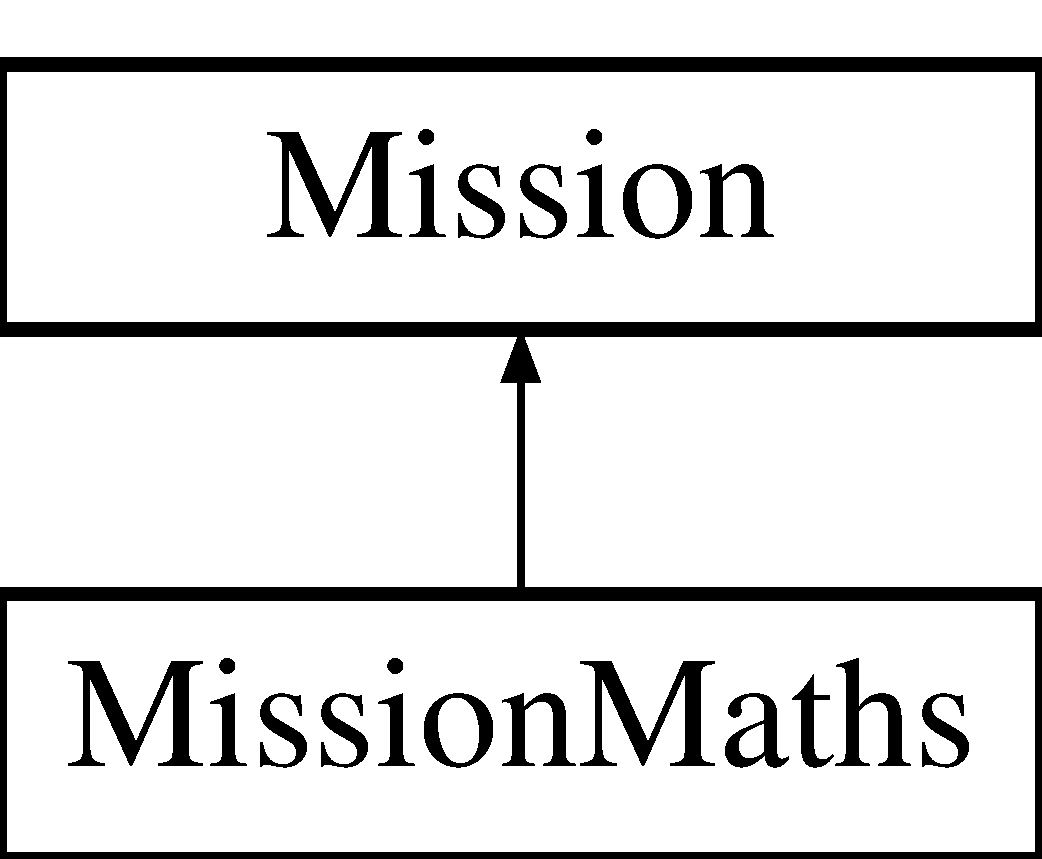
\includegraphics[height=2.000000cm]{class_mission_maths}
\end{center}
\end{figure}
\subsection*{Public Member Functions}
\begin{DoxyCompactItemize}
\item 
\hyperlink{class_mission_maths_abe58873e14c757c086ecaf42e581dd20}{Mission\-Maths} ()
\begin{DoxyCompactList}\small\item\em Constructeur par défaut. \end{DoxyCompactList}\item 
\hyperlink{class_mission_maths_afd5e073b7a77121cf692925f71b27959}{Mission\-Maths} (int acc\-Intel, int acc\-Force, int acc\-Age, int acc\-Energie, string nom, int rec\-Intel, string dialogue\-R, string dialogue\-E)
\begin{DoxyCompactList}\small\item\em Constructeur de la classe mission maths. \end{DoxyCompactList}\item 
void \hyperlink{class_mission_maths_a29c16120131c778ab70c67f26252ff0c}{set\-Recomp\-Int} (int new\-\_\-var)
\begin{DoxyCompactList}\small\item\em stock la valeur de la variable new\-\_\-var dans la variable recomp\-Int. \end{DoxyCompactList}\item 
int \hyperlink{class_mission_maths_a43e24544f6550d8acffb0fd19eefe3a5}{get\-Recomp\-Int} ()
\begin{DoxyCompactList}\small\item\em Accède à la variable recomp\-Int. \end{DoxyCompactList}\item 
void \hyperlink{class_mission_maths_a07c256993831514508290420b4b57bcf}{set\-Question} (vector$<$ \hyperlink{struct_q_c_m}{Q\-C\-M} $>$ new\-\_\-var)
\begin{DoxyCompactList}\small\item\em stock la valeur de la variable new\-\_\-var dans la variable question. \end{DoxyCompactList}\item 
vector$<$ \hyperlink{struct_q_c_m}{Q\-C\-M} $>$ \hyperlink{class_mission_maths_a719d59e5c73f690c92417863cec4e747}{get\-Question} ()
\begin{DoxyCompactList}\small\item\em Accède à la variable question. \end{DoxyCompactList}\item 
string \hyperlink{class_mission_maths_a0cc9fd94da2659ec7274693097e93bd3}{get\-Nom\-Mission} ()
\begin{DoxyCompactList}\small\item\em Accède à la variable nom\-Mission. \end{DoxyCompactList}\item 
void \hyperlink{class_mission_maths_a238579d120711f3be1ca9254a5cad214}{set\-Nom\-Mission} (string var)
\begin{DoxyCompactList}\small\item\em stock la valeur de la variable var dans la variable nom\-Mission. \end{DoxyCompactList}\item 
string \hyperlink{class_mission_maths_aec614bc24cbe313c5ce6d5d76119a041}{executer\-Mission} (\hyperlink{class_jeu}{Jeu} jeu, \hyperlink{class_heros}{Heros} $\ast$heros, \hyperlink{class_p_n_j}{P\-N\-J} $\ast$pnj)
\begin{DoxyCompactList}\small\item\em Exécute une mission de type maths. \end{DoxyCompactList}\end{DoxyCompactItemize}
\subsection*{Additional Inherited Members}


\subsection{Detailed Description}
Classe représentant les missions de type maths. 

\subsection{Constructor \& Destructor Documentation}
\hypertarget{class_mission_maths_abe58873e14c757c086ecaf42e581dd20}{\index{Mission\-Maths@{Mission\-Maths}!Mission\-Maths@{Mission\-Maths}}
\index{Mission\-Maths@{Mission\-Maths}!MissionMaths@{Mission\-Maths}}
\subsubsection[{Mission\-Maths}]{\setlength{\rightskip}{0pt plus 5cm}Mission\-Maths\-::\-Mission\-Maths (
\begin{DoxyParamCaption}
{}
\end{DoxyParamCaption}
)}}\label{class_mission_maths_abe58873e14c757c086ecaf42e581dd20}


Constructeur par défaut. 


\begin{DoxyCode}
15 \{\}
\end{DoxyCode}
\hypertarget{class_mission_maths_afd5e073b7a77121cf692925f71b27959}{\index{Mission\-Maths@{Mission\-Maths}!Mission\-Maths@{Mission\-Maths}}
\index{Mission\-Maths@{Mission\-Maths}!MissionMaths@{Mission\-Maths}}
\subsubsection[{Mission\-Maths}]{\setlength{\rightskip}{0pt plus 5cm}Mission\-Maths\-::\-Mission\-Maths (
\begin{DoxyParamCaption}
\item[{int}]{acc\-Intel, }
\item[{int}]{acc\-Force, }
\item[{int}]{acc\-Age, }
\item[{int}]{acc\-Energie, }
\item[{string}]{nom, }
\item[{int}]{rec\-Intel, }
\item[{string}]{dialogue\-R, }
\item[{string}]{dialogue\-E}
\end{DoxyParamCaption}
)}}\label{class_mission_maths_afd5e073b7a77121cf692925f71b27959}


Constructeur de la classe mission maths. 


\begin{DoxyParams}{Parameters}
{\em heros} & Un paramètre de la classe \hyperlink{class_heros}{Heros}. \\
\hline
{\em acc\-Intel} & La valeur nécessaire d'intelligence pour accéder à une mission. \\
\hline
{\em acc\-Force} & La valeur nécessaire de la force pour accéder à une mission. \\
\hline
{\em acc\-Age} & La valeur nécessaire d'âge pour accéder à une mission. \\
\hline
{\em access\-Energie} & La valeur nécessaire d'énergie pour accéder à une mission. \\
\hline
{\em nom} & le nom de la mission. \\
\hline
{\em rec\-Intel} & La valeur de la récompense intelligence que l'héros peut gagner. \\
\hline
{\em dialogue\-R} & Le dialogue en cas de réussite. \\
\hline
{\em dialogue\-E} & Le dialogue en cas d'échec. \\
\hline
\end{DoxyParams}

\begin{DoxyCode}
16                                                                                                            
                                         : \hyperlink{class_mission_aa5a6ff4fc779338ab01b8f6dd470f4df}{Mission}(accIntel,accForce,accAge,accEnergie,nom, dialogueR, 
      dialogueE)\{
17     recompInt = recIntel;
18     niveau = floor(\hyperlink{class_mission_af93302ac38548302411994e4cbf9b850}{accessIntel}/10);
19 
20     \}
\end{DoxyCode}


\subsection{Member Function Documentation}
\hypertarget{class_mission_maths_aec614bc24cbe313c5ce6d5d76119a041}{\index{Mission\-Maths@{Mission\-Maths}!executer\-Mission@{executer\-Mission}}
\index{executer\-Mission@{executer\-Mission}!MissionMaths@{Mission\-Maths}}
\subsubsection[{executer\-Mission}]{\setlength{\rightskip}{0pt plus 5cm}string Mission\-Maths\-::executer\-Mission (
\begin{DoxyParamCaption}
\item[{{\bf Jeu}}]{jeu, }
\item[{{\bf Heros} $\ast$}]{heros, }
\item[{{\bf P\-N\-J} $\ast$}]{pnj}
\end{DoxyParamCaption}
)\hspace{0.3cm}{\ttfamily [virtual]}}}\label{class_mission_maths_aec614bc24cbe313c5ce6d5d76119a041}


Exécute une mission de type maths. 


\begin{DoxyParams}{Parameters}
{\em jeu} & Une instance de la classe \hyperlink{class_jeu}{Jeu}. \\
\hline
{\em heros} & Un pointeur sur la classe \hyperlink{class_heros}{Heros}. \\
\hline
{\em pnj} & Un pointeur sur la classe \hyperlink{class_p_n_j}{P\-N\-J}. \\
\hline
\end{DoxyParams}
\begin{DoxyReturn}{Returns}
Un message permettant de savoir si le héros a réussi ou échoué la mission maths et combien de points d'intelligence a-\/t-\/il gagné etc. 
\end{DoxyReturn}


Reimplemented from \hyperlink{class_mission_ad4375f925eda8637d6346ef468747f44}{Mission}.


\begin{DoxyCode}
38                                                                       \{
39 
40       \textcolor{keywordflow}{if} (heros->\hyperlink{class_heros_ae9bbef6d2edcb8b14d9ec3854146a42c}{getEnergie}()> \hyperlink{class_mission_ae767714f7433f66f519468bc1913a5ef}{accessEnergie}) \{
41 
42       \textcolor{keywordflow}{if} (jeu.\hyperlink{class_jeu_a3aa07b1e7a5e5d82479b8bb2a2841635}{demanderBoolUtilisateur}(\textcolor{stringliteral}{"Voulez vous essayer de répondre à une
       question de niveau "}+\hyperlink{missionmaths_8cpp_a0d2f37137ee1fd6ff4a0ef803849dd63}{SSTR}(niveau)+\textcolor{stringliteral}{" ? Vous gagnerez ainsi "}+\hyperlink{missionmaths_8cpp_a0d2f37137ee1fd6ff4a0ef803849dd63}{SSTR}(recompInt)+\textcolor{stringliteral}{" points d'intelligence"} ))\{
43           \hyperlink{class_mission_a5ee38d2b67b7f860fb6a27d486200bec}{setEtatMission}(\hyperlink{mission_8hpp_ace9df1e8554ba5a57340fb42cee370f7aca12092e4757cb029f1b3e1fa95ed277}{enCours});
44 
45               heros->\hyperlink{class_heros_a5d4f5d3d3a4db451923f0609a3e1b53c}{setEnergie}(heros->\hyperlink{class_heros_ae9bbef6d2edcb8b14d9ec3854146a42c}{getEnergie}()-
      \hyperlink{class_mission_ae767714f7433f66f519468bc1913a5ef}{accessEnergie});
46               jeu.\hyperlink{class_jeu_aa09fb40439f16b9665a0d76679f78e4e}{afficherTexte}(\textcolor{stringliteral}{"Vous venez de perdre "}+\hyperlink{missionmaths_8cpp_a0d2f37137ee1fd6ff4a0ef803849dd63}{SSTR}(
      \hyperlink{class_mission_ae767714f7433f66f519468bc1913a5ef}{accessEnergie})+\textcolor{stringliteral}{" points d'énergie, il vous en reste "}+\hyperlink{missionmaths_8cpp_a0d2f37137ee1fd6ff4a0ef803849dd63}{SSTR}(heros->
      \hyperlink{class_heros_ae9bbef6d2edcb8b14d9ec3854146a42c}{getEnergie}()));
47               jeu.\hyperlink{class_jeu_a52ce4fb6c415b45209db13a589c9d675}{timer}(1,\textcolor{stringliteral}{""});
48               jeu.\hyperlink{class_jeu_a52ce4fb6c415b45209db13a589c9d675}{timer}(3,pnj->\hyperlink{class_personnage_a519301399a9bee1557858aa50a04a85a}{getNom}()+\textcolor{stringliteral}{" : Laisse moi réfléchir à une question..."});
49 
50           \textcolor{keywordtype}{bool} test = \textcolor{keyword}{true};
51           \textcolor{keywordflow}{for}(\textcolor{keywordtype}{int} i=0; i<question.size() and test==\textcolor{keyword}{true}; i++)\{
52               \textcolor{keywordtype}{int} entree = jeu.\hyperlink{class_jeu_ac504a2a26ad7aa3c4281f8ab40cdc445}{demanderEntreeUtilisateur}(question.at(i).exo);
53               \textcolor{keywordflow}{if} (entree != question.at(i).answer) \{
54                   test = \textcolor{keyword}{false};
55                   jeu.\hyperlink{class_jeu_a52ce4fb6c415b45209db13a589c9d675}{timer}(2,pnj->\hyperlink{class_personnage_a519301399a9bee1557858aa50a04a85a}{getNom}()+\textcolor{stringliteral}{" : Pas du tout ! C'est médiocre ! On s'arrête là."})
      ;
56               \}
57               \textcolor{keywordflow}{else} \textcolor{keywordflow}{if} (i!= question.size()-1) jeu.\hyperlink{class_jeu_a52ce4fb6c415b45209db13a589c9d675}{timer}(3,pnj->\hyperlink{class_personnage_a519301399a9bee1557858aa50a04a85a}{getNom}()+\textcolor{stringliteral}{" : hum... celle là
       était simple. Laisse moi réfléchir à une autre question."});
58           \}
59           \textcolor{keywordflow}{if} (test==\textcolor{keyword}{true}) \{
60             heros->\hyperlink{class_personnage_af8b3c4f6c0f7035678d9ecf574976650}{setIntelligence}(heros->\hyperlink{class_personnage_a250eec1aba0df7a105dd564e4cd02b0b}{getIntelligence}()+recompInt);
61             \textcolor{keywordflow}{return} pnj->\hyperlink{class_personnage_a519301399a9bee1557858aa50a04a85a}{getNom}()+\textcolor{stringliteral}{" : "}+\hyperlink{class_mission_adedaca4409d2abe41a36c04921440b86}{getDialogueReussite}()+\textcolor{stringliteral}{"\(\backslash\)nVous avez gagné "}+
      \hyperlink{missionmaths_8cpp_a0d2f37137ee1fd6ff4a0ef803849dd63}{SSTR}(recompInt)+\textcolor{stringliteral}{" de points d'intelligence"};
62             \}
63           \textcolor{keywordflow}{else}
64             \textcolor{keywordflow}{return} \hyperlink{class_mission_af9a813bba373bcac25b42e22c8440c1c}{getDialogueEchec}();
65           \}
66       \textcolor{keywordflow}{else} \textcolor{keywordflow}{return} pnj->\hyperlink{class_personnage_a519301399a9bee1557858aa50a04a85a}{getNom}()+\textcolor{stringliteral}{" : Je vois... Vous n'êtes donc pas de taille... Amateur."};
67       \}
68       \textcolor{keywordflow}{else} \textcolor{keywordflow}{return} \textcolor{stringliteral}{"Vous n'avez pas assez d'énergie... Dommage."};
69   \}
\end{DoxyCode}
\hypertarget{class_mission_maths_a0cc9fd94da2659ec7274693097e93bd3}{\index{Mission\-Maths@{Mission\-Maths}!get\-Nom\-Mission@{get\-Nom\-Mission}}
\index{get\-Nom\-Mission@{get\-Nom\-Mission}!MissionMaths@{Mission\-Maths}}
\subsubsection[{get\-Nom\-Mission}]{\setlength{\rightskip}{0pt plus 5cm}string Mission\-Maths\-::get\-Nom\-Mission (
\begin{DoxyParamCaption}
{}
\end{DoxyParamCaption}
)}}\label{class_mission_maths_a0cc9fd94da2659ec7274693097e93bd3}


Accède à la variable nom\-Mission. 

\begin{DoxyReturn}{Returns}
Le nom de la mission. 
\end{DoxyReturn}
\hypertarget{class_mission_maths_a719d59e5c73f690c92417863cec4e747}{\index{Mission\-Maths@{Mission\-Maths}!get\-Question@{get\-Question}}
\index{get\-Question@{get\-Question}!MissionMaths@{Mission\-Maths}}
\subsubsection[{get\-Question}]{\setlength{\rightskip}{0pt plus 5cm}vector$<$ {\bf Q\-C\-M} $>$ Mission\-Maths\-::get\-Question (
\begin{DoxyParamCaption}
{}
\end{DoxyParamCaption}
)}}\label{class_mission_maths_a719d59e5c73f690c92417863cec4e747}


Accède à la variable question. 

\begin{DoxyReturn}{Returns}
Le vecteur des questions composé de l'exercice et la réponse. 
\end{DoxyReturn}

\begin{DoxyCode}
34                                              \{
35     \textcolor{keywordflow}{return} question;
36   \}
\end{DoxyCode}
\hypertarget{class_mission_maths_a43e24544f6550d8acffb0fd19eefe3a5}{\index{Mission\-Maths@{Mission\-Maths}!get\-Recomp\-Int@{get\-Recomp\-Int}}
\index{get\-Recomp\-Int@{get\-Recomp\-Int}!MissionMaths@{Mission\-Maths}}
\subsubsection[{get\-Recomp\-Int}]{\setlength{\rightskip}{0pt plus 5cm}int Mission\-Maths\-::get\-Recomp\-Int (
\begin{DoxyParamCaption}
{}
\end{DoxyParamCaption}
)}}\label{class_mission_maths_a43e24544f6550d8acffb0fd19eefe3a5}


Accède à la variable recomp\-Int. 

\begin{DoxyReturn}{Returns}
la valeur de la récompense intelligence. 
\end{DoxyReturn}

\begin{DoxyCode}
26                                       \{
27     \textcolor{keywordflow}{return} recompInt;
28   \}
\end{DoxyCode}
\hypertarget{class_mission_maths_a238579d120711f3be1ca9254a5cad214}{\index{Mission\-Maths@{Mission\-Maths}!set\-Nom\-Mission@{set\-Nom\-Mission}}
\index{set\-Nom\-Mission@{set\-Nom\-Mission}!MissionMaths@{Mission\-Maths}}
\subsubsection[{set\-Nom\-Mission}]{\setlength{\rightskip}{0pt plus 5cm}void Mission\-Maths\-::set\-Nom\-Mission (
\begin{DoxyParamCaption}
\item[{string}]{var}
\end{DoxyParamCaption}
)}}\label{class_mission_maths_a238579d120711f3be1ca9254a5cad214}


stock la valeur de la variable var dans la variable nom\-Mission. 

\hypertarget{class_mission_maths_a07c256993831514508290420b4b57bcf}{\index{Mission\-Maths@{Mission\-Maths}!set\-Question@{set\-Question}}
\index{set\-Question@{set\-Question}!MissionMaths@{Mission\-Maths}}
\subsubsection[{set\-Question}]{\setlength{\rightskip}{0pt plus 5cm}void Mission\-Maths\-::set\-Question (
\begin{DoxyParamCaption}
\item[{vector$<$ {\bf Q\-C\-M} $>$}]{new\-\_\-var}
\end{DoxyParamCaption}
)}}\label{class_mission_maths_a07c256993831514508290420b4b57bcf}


stock la valeur de la variable new\-\_\-var dans la variable question. 


\begin{DoxyCode}
30                                                          \{
31       question = new\_var;
32   \}
\end{DoxyCode}
\hypertarget{class_mission_maths_a29c16120131c778ab70c67f26252ff0c}{\index{Mission\-Maths@{Mission\-Maths}!set\-Recomp\-Int@{set\-Recomp\-Int}}
\index{set\-Recomp\-Int@{set\-Recomp\-Int}!MissionMaths@{Mission\-Maths}}
\subsubsection[{set\-Recomp\-Int}]{\setlength{\rightskip}{0pt plus 5cm}void Mission\-Maths\-::set\-Recomp\-Int (
\begin{DoxyParamCaption}
\item[{int}]{new\-\_\-var}
\end{DoxyParamCaption}
)}}\label{class_mission_maths_a29c16120131c778ab70c67f26252ff0c}


stock la valeur de la variable new\-\_\-var dans la variable recomp\-Int. 


\begin{DoxyCode}
22                                                  \{
23       recompInt = new\_var;
24   \}
\end{DoxyCode}


The documentation for this class was generated from the following files\-:\begin{DoxyCompactItemize}
\item 
/nfs/usersgm/\-G\-M26/neljibbawe/\-Bureau/\-Projet\-C\-P\-P\-A\-Rendre/\-C\-P\-P R\-P\-G/\-R\-P\-G/\hyperlink{missionmaths_8hpp}{missionmaths.\-hpp}\item 
/nfs/usersgm/\-G\-M26/neljibbawe/\-Bureau/\-Projet\-C\-P\-P\-A\-Rendre/\-C\-P\-P R\-P\-G/\-R\-P\-G/\hyperlink{missionmaths_8cpp}{missionmaths.\-cpp}\end{DoxyCompactItemize}

\hypertarget{class_mission_objet}{\section{Mission\-Objet Class Reference}
\label{class_mission_objet}\index{Mission\-Objet@{Mission\-Objet}}
}


Classe représentant les missions de type objet.  




{\ttfamily \#include $<$missionobjet.\-hpp$>$}

Inheritance diagram for Mission\-Objet\-:\begin{figure}[H]
\begin{center}
\leavevmode
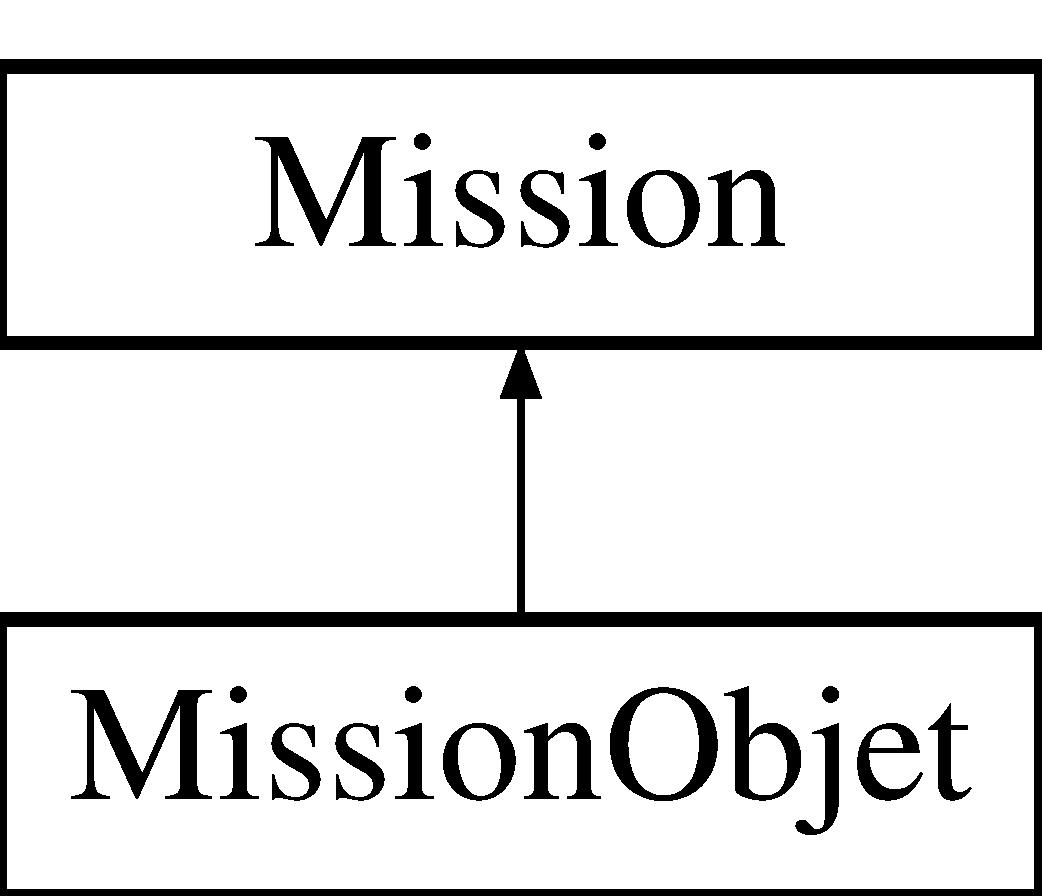
\includegraphics[height=2.000000cm]{class_mission_objet}
\end{center}
\end{figure}
\subsection*{Public Member Functions}
\begin{DoxyCompactItemize}
\item 
\hyperlink{class_mission_objet_a318a1e74b1c2fb4a5c4f9e8c1307cb5d}{Mission\-Objet} ()
\begin{DoxyCompactList}\small\item\em Constructeur par défaut. \end{DoxyCompactList}\item 
\hyperlink{class_mission_objet_a3622eac0551933b75a5d11c93ceba22f}{Mission\-Objet} (int acc\-Intel, int acc\-Force, int acc\-Age, int acc\-Energie, string nom, int rec\-Cash, string dialogue\-R, string dialogue\-E, \hyperlink{class_objet}{Objet} obj\-Rec, \hyperlink{class_objet}{Objet} obj\-A\-Trouver)
\begin{DoxyCompactList}\small\item\em Constructeur de la classe mission objet. \end{DoxyCompactList}\item 
void \hyperlink{class_mission_objet_ac8de7ea7c712f4f5db299909043a18b9}{set\-Recomp\-Cash} (int new\-\_\-var)
\begin{DoxyCompactList}\small\item\em stock la valeur de la variable new\-\_\-var dans la variable recomp\-Cash. \end{DoxyCompactList}\item 
int \hyperlink{class_mission_objet_af488361b1557fe4443494479fb5b1861}{get\-Recomp\-Cash} ()
\begin{DoxyCompactList}\small\item\em Accède à la variable recomp\-Cash. \end{DoxyCompactList}\item 
void \hyperlink{class_mission_objet_a0c3e3707924333f8de5b236d172191de}{set\-Recomp\-Objet} (\hyperlink{class_objet}{Objet} new\-\_\-var)
\begin{DoxyCompactList}\small\item\em stock la valeur de la variable new\-\_\-var dans la variable recomp\-Objet. \end{DoxyCompactList}\item 
\hyperlink{class_objet}{Objet} \hyperlink{class_mission_objet_a2bf5716c0c4cb7b6a9239af4c083d26d}{get\-Recomp\-Objet} ()
\begin{DoxyCompactList}\small\item\em Accède à la variable recomp\-Objet. \end{DoxyCompactList}\item 
string \hyperlink{class_mission_objet_a77d2258493308443e34c27beefc6b6e0}{get\-Nom\-Mission} ()
\begin{DoxyCompactList}\small\item\em Accède à la variable nom\-Mission. \end{DoxyCompactList}\item 
void \hyperlink{class_mission_objet_a62531c502fbc5fb1d5634a69afeaa3d3}{set\-Nom\-Mission} (string var)
\begin{DoxyCompactList}\small\item\em stock la valeur de la variable var dans la variable nom\-Mission. \end{DoxyCompactList}\item 
string \hyperlink{class_mission_objet_a49547f2e562b288a9abd640641964f78}{executer\-Mission} (\hyperlink{class_jeu}{Jeu} jeu, \hyperlink{class_heros}{Heros} $\ast$heros, \hyperlink{class_p_n_j}{P\-N\-J} $\ast$pnj)
\begin{DoxyCompactList}\small\item\em Exécute une mission de type objet. \end{DoxyCompactList}\end{DoxyCompactItemize}
\subsection*{Additional Inherited Members}


\subsection{Detailed Description}
Classe représentant les missions de type objet. 

\subsection{Constructor \& Destructor Documentation}
\hypertarget{class_mission_objet_a318a1e74b1c2fb4a5c4f9e8c1307cb5d}{\index{Mission\-Objet@{Mission\-Objet}!Mission\-Objet@{Mission\-Objet}}
\index{Mission\-Objet@{Mission\-Objet}!MissionObjet@{Mission\-Objet}}
\subsubsection[{Mission\-Objet}]{\setlength{\rightskip}{0pt plus 5cm}Mission\-Objet\-::\-Mission\-Objet (
\begin{DoxyParamCaption}
{}
\end{DoxyParamCaption}
)}}\label{class_mission_objet_a318a1e74b1c2fb4a5c4f9e8c1307cb5d}


Constructeur par défaut. 


\begin{DoxyCode}
15 \{\}
\end{DoxyCode}
\hypertarget{class_mission_objet_a3622eac0551933b75a5d11c93ceba22f}{\index{Mission\-Objet@{Mission\-Objet}!Mission\-Objet@{Mission\-Objet}}
\index{Mission\-Objet@{Mission\-Objet}!MissionObjet@{Mission\-Objet}}
\subsubsection[{Mission\-Objet}]{\setlength{\rightskip}{0pt plus 5cm}Mission\-Objet\-::\-Mission\-Objet (
\begin{DoxyParamCaption}
\item[{int}]{acc\-Intel, }
\item[{int}]{acc\-Force, }
\item[{int}]{acc\-Age, }
\item[{int}]{acc\-Energie, }
\item[{string}]{nom, }
\item[{int}]{rec\-Cash, }
\item[{string}]{dialogue\-R, }
\item[{string}]{dialogue\-E, }
\item[{{\bf Objet}}]{obj\-Rec, }
\item[{{\bf Objet}}]{obj\-A\-Trouver}
\end{DoxyParamCaption}
)}}\label{class_mission_objet_a3622eac0551933b75a5d11c93ceba22f}


Constructeur de la classe mission objet. 


\begin{DoxyParams}{Parameters}
{\em acc\-Intel} & La valeur nécessaire d'intelligence pour accéder à une mission. \\
\hline
{\em acc\-Force} & La valeur nécessaire de la force pour accéder à une mission. \\
\hline
{\em acc\-Age} & La valeur nécessaire d'âge pour accéder à une mission. \\
\hline
{\em access\-Energie} & La valeur nécessaire d'énergie pour accéder à une mission. \\
\hline
{\em nom} & Le nom de la mission. \\
\hline
{\em rec\-Cash} & La valeur de la récompense cash que l'héros peut gagner. \\
\hline
{\em dialogue\-R} & Le dialogue en cas de réussite. \\
\hline
{\em dialogue\-E} & Le dialogue en cas d'échec. \\
\hline
{\em obj\-Rec} & L'objet que l'héros peut gagner. \\
\hline
{\em obj\-A\-Trouver} & L'objet que l'héros doit trouver. \\
\hline
\end{DoxyParams}

\begin{DoxyCode}
16                                                                                                            
                                                                       : \hyperlink{class_mission_aa5a6ff4fc779338ab01b8f6dd470f4df}{Mission}(accIntel,accForce,accAge,
      accEnergie,nom, dialogueR, dialogueE)\{
17     recompCash = recCash;
18     recompObjet = objRec;
19     objetATrouver = objATrouver;
20     \}
\end{DoxyCode}


\subsection{Member Function Documentation}
\hypertarget{class_mission_objet_a49547f2e562b288a9abd640641964f78}{\index{Mission\-Objet@{Mission\-Objet}!executer\-Mission@{executer\-Mission}}
\index{executer\-Mission@{executer\-Mission}!MissionObjet@{Mission\-Objet}}
\subsubsection[{executer\-Mission}]{\setlength{\rightskip}{0pt plus 5cm}string Mission\-Objet\-::executer\-Mission (
\begin{DoxyParamCaption}
\item[{{\bf Jeu}}]{jeu, }
\item[{{\bf Heros} $\ast$}]{heros, }
\item[{{\bf P\-N\-J} $\ast$}]{pnj}
\end{DoxyParamCaption}
)\hspace{0.3cm}{\ttfamily [virtual]}}}\label{class_mission_objet_a49547f2e562b288a9abd640641964f78}


Exécute une mission de type objet. 


\begin{DoxyParams}{Parameters}
{\em jeu} & Une instance de la classe \hyperlink{class_jeu}{Jeu}. \\
\hline
{\em heros} & Un pointeur sur la classe \hyperlink{class_heros}{Heros}. \\
\hline
{\em pnj} & Un pointeur sur la classe \hyperlink{class_p_n_j}{P\-N\-J}. \\
\hline
\end{DoxyParams}
\begin{DoxyReturn}{Returns}
Un texte permettant de savoir si le héros a assez d'énergie pour faire ce type de mission, s'il a réussi ou échoué à faire cette mission etc. 
\end{DoxyReturn}


Reimplemented from \hyperlink{class_mission_ad4375f925eda8637d6346ef468747f44}{Mission}.


\begin{DoxyCode}
38                                                                      \{
39       \textcolor{keywordflow}{if}(jeu.\hyperlink{class_jeu_a3aa07b1e7a5e5d82479b8bb2a2841635}{demanderBoolUtilisateur}(\hyperlink{class_mission_ad6b21ef20ff04bad9769f3b50a3b1218}{getTexteMission}())) \{
40       \textcolor{keywordflow}{if} (\hyperlink{class_mission_aa513084d347dc1c4c8a957258c9d3876}{getEtatMission}() != \hyperlink{mission_8hpp_ace9df1e8554ba5a57340fb42cee370f7aca12092e4757cb029f1b3e1fa95ed277}{enCours})\{
41           \hyperlink{class_mission_a5ee38d2b67b7f860fb6a27d486200bec}{setEtatMission}(\hyperlink{mission_8hpp_ace9df1e8554ba5a57340fb42cee370f7aca12092e4757cb029f1b3e1fa95ed277}{enCours});
42           \textcolor{keywordflow}{if} (heros->\hyperlink{class_heros_ae9bbef6d2edcb8b14d9ec3854146a42c}{getEnergie}()> \hyperlink{class_mission_ae767714f7433f66f519468bc1913a5ef}{accessEnergie}) \{
43               heros->\hyperlink{class_heros_a5d4f5d3d3a4db451923f0609a3e1b53c}{setEnergie}(heros->\hyperlink{class_heros_ae9bbef6d2edcb8b14d9ec3854146a42c}{getEnergie}()-
      \hyperlink{class_mission_ae767714f7433f66f519468bc1913a5ef}{accessEnergie});
44               jeu.\hyperlink{class_jeu_a52ce4fb6c415b45209db13a589c9d675}{timer}(3,\textcolor{stringliteral}{"Nouvelle mission : vous avez perdu "}+\hyperlink{missionobjet_8cpp_a0d2f37137ee1fd6ff4a0ef803849dd63}{SSTR}(
      \hyperlink{class_mission_ae767714f7433f66f519468bc1913a5ef}{accessEnergie})+\textcolor{stringliteral}{" d'énergie."});
45 
46           \}
47           \textcolor{keywordflow}{else} \{
48               \textcolor{keywordflow}{return} \textcolor{stringliteral}{"Vous n'avez pas assez d'énergie, dommage."};
49           \}
50 
51       \}
52       \textcolor{keywordflow}{else} jeu.\hyperlink{class_jeu_a52ce4fb6c415b45209db13a589c9d675}{timer}(4,pnj->\hyperlink{class_personnage_a519301399a9bee1557858aa50a04a85a}{getNom}()+\textcolor{stringliteral}{" : Alors, tu as retrouvé : ("}+objetATrouver.
      \hyperlink{class_objet_a843e99ecd1e150589f8db23f43dd27b0}{getNomObjet}()+\textcolor{stringliteral}{") ?\(\backslash\)n Vous cherchez dans votre sac..."});
53 
54         map<string,Objet*> sacHeros = heros->\hyperlink{class_heros_a62d8b172e82dbb0a1d2c23da21bdb069}{getSac}();
55 
56         \textcolor{keywordflow}{if} (sacHeros[objetATrouver.\hyperlink{class_objet_a843e99ecd1e150589f8db23f43dd27b0}{getNomObjet}()]->getQuantiteObjet()>0)\{
57 
58             sacHeros[objetATrouver.\hyperlink{class_objet_a843e99ecd1e150589f8db23f43dd27b0}{getNomObjet}()]->setQuantiteObjet(sacHeros[objetATrouver.
      \hyperlink{class_objet_a843e99ecd1e150589f8db23f43dd27b0}{getNomObjet}()]->getQuantiteObjet()-1);
59 
60             sacHeros[recompObjet.\hyperlink{class_objet_a843e99ecd1e150589f8db23f43dd27b0}{getNomObjet}()]->setQuantiteObjet(sacHeros[recompObjet.
      \hyperlink{class_objet_a843e99ecd1e150589f8db23f43dd27b0}{getNomObjet}()]->getQuantiteObjet()+1);
61 
62             heros->\hyperlink{class_heros_a7d6d86388fe81deca1c5688ed07b2167}{setSac}(sacHeros);
63             \hyperlink{class_mission_a5ee38d2b67b7f860fb6a27d486200bec}{setEtatMission}(\hyperlink{mission_8hpp_ace9df1e8554ba5a57340fb42cee370f7a9e765bd835523da043a754ce21905cb5}{achevee});
64             heros->\hyperlink{class_heros_ae87dba7afa03e7fdacfc3a7e82d3a6a3}{setCash}(heros->\hyperlink{class_heros_a77bdee21cb8c8356448bb6669941441c}{getCash}()+recompCash);
65             jeu.\hyperlink{class_jeu_a52ce4fb6c415b45209db13a589c9d675}{timer}(3,\textcolor{stringliteral}{"Vous avez obtenu "}+\hyperlink{missionobjet_8cpp_a0d2f37137ee1fd6ff4a0ef803849dd63}{SSTR}(recompCash)+\textcolor{stringliteral}{" cash et l'objet suivant : ("}+
      recompObjet.\hyperlink{class_objet_a843e99ecd1e150589f8db23f43dd27b0}{getNomObjet}()+\textcolor{stringliteral}{")"});
66             \textcolor{keywordflow}{return} \hyperlink{class_mission_a75d8fc66d0ed01f1f1192e03528a2612}{dialogueReussite};
67         \}
68 
69         \textcolor{keywordflow}{else} \{
70             \textcolor{keywordflow}{return} \hyperlink{class_mission_aeb543b4e12125834e6b8901820db243b}{dialogueEchec};
71         \}
72       \}
73       \textcolor{keywordflow}{else} \{
74           jeu.\hyperlink{class_jeu_a52ce4fb6c415b45209db13a589c9d675}{timer}(3,\textcolor{stringliteral}{"Reviens me voir si tu changes d'avis"});
75           \textcolor{keywordflow}{return} \textcolor{stringliteral}{""};
76       \}
77   \}
\end{DoxyCode}
\hypertarget{class_mission_objet_a77d2258493308443e34c27beefc6b6e0}{\index{Mission\-Objet@{Mission\-Objet}!get\-Nom\-Mission@{get\-Nom\-Mission}}
\index{get\-Nom\-Mission@{get\-Nom\-Mission}!MissionObjet@{Mission\-Objet}}
\subsubsection[{get\-Nom\-Mission}]{\setlength{\rightskip}{0pt plus 5cm}string Mission\-Objet\-::get\-Nom\-Mission (
\begin{DoxyParamCaption}
{}
\end{DoxyParamCaption}
)}}\label{class_mission_objet_a77d2258493308443e34c27beefc6b6e0}


Accède à la variable nom\-Mission. 

\begin{DoxyReturn}{Returns}
Le nom de la mission. 
\end{DoxyReturn}
\hypertarget{class_mission_objet_af488361b1557fe4443494479fb5b1861}{\index{Mission\-Objet@{Mission\-Objet}!get\-Recomp\-Cash@{get\-Recomp\-Cash}}
\index{get\-Recomp\-Cash@{get\-Recomp\-Cash}!MissionObjet@{Mission\-Objet}}
\subsubsection[{get\-Recomp\-Cash}]{\setlength{\rightskip}{0pt plus 5cm}int Mission\-Objet\-::get\-Recomp\-Cash (
\begin{DoxyParamCaption}
{}
\end{DoxyParamCaption}
)}}\label{class_mission_objet_af488361b1557fe4443494479fb5b1861}


Accède à la variable recomp\-Cash. 

\begin{DoxyReturn}{Returns}
la valeur de la récompense cash. 
\end{DoxyReturn}

\begin{DoxyCode}
26                                        \{
27     \textcolor{keywordflow}{return} recompCash;
28   \}
\end{DoxyCode}
\hypertarget{class_mission_objet_a2bf5716c0c4cb7b6a9239af4c083d26d}{\index{Mission\-Objet@{Mission\-Objet}!get\-Recomp\-Objet@{get\-Recomp\-Objet}}
\index{get\-Recomp\-Objet@{get\-Recomp\-Objet}!MissionObjet@{Mission\-Objet}}
\subsubsection[{get\-Recomp\-Objet}]{\setlength{\rightskip}{0pt plus 5cm}{\bf Objet} Mission\-Objet\-::get\-Recomp\-Objet (
\begin{DoxyParamCaption}
{}
\end{DoxyParamCaption}
)}}\label{class_mission_objet_a2bf5716c0c4cb7b6a9239af4c083d26d}


Accède à la variable recomp\-Objet. 

\begin{DoxyReturn}{Returns}
l'objet correspondant à la récompense objet. 
\end{DoxyReturn}

\begin{DoxyCode}
34                                           \{
35     \textcolor{keywordflow}{return} recompObjet;
36   \}
\end{DoxyCode}
\hypertarget{class_mission_objet_a62531c502fbc5fb1d5634a69afeaa3d3}{\index{Mission\-Objet@{Mission\-Objet}!set\-Nom\-Mission@{set\-Nom\-Mission}}
\index{set\-Nom\-Mission@{set\-Nom\-Mission}!MissionObjet@{Mission\-Objet}}
\subsubsection[{set\-Nom\-Mission}]{\setlength{\rightskip}{0pt plus 5cm}void Mission\-Objet\-::set\-Nom\-Mission (
\begin{DoxyParamCaption}
\item[{string}]{var}
\end{DoxyParamCaption}
)}}\label{class_mission_objet_a62531c502fbc5fb1d5634a69afeaa3d3}


stock la valeur de la variable var dans la variable nom\-Mission. 

\hypertarget{class_mission_objet_ac8de7ea7c712f4f5db299909043a18b9}{\index{Mission\-Objet@{Mission\-Objet}!set\-Recomp\-Cash@{set\-Recomp\-Cash}}
\index{set\-Recomp\-Cash@{set\-Recomp\-Cash}!MissionObjet@{Mission\-Objet}}
\subsubsection[{set\-Recomp\-Cash}]{\setlength{\rightskip}{0pt plus 5cm}void Mission\-Objet\-::set\-Recomp\-Cash (
\begin{DoxyParamCaption}
\item[{int}]{new\-\_\-var}
\end{DoxyParamCaption}
)}}\label{class_mission_objet_ac8de7ea7c712f4f5db299909043a18b9}


stock la valeur de la variable new\-\_\-var dans la variable recomp\-Cash. 


\begin{DoxyCode}
22                                                   \{
23       recompCash = new\_var;
24   \}
\end{DoxyCode}
\hypertarget{class_mission_objet_a0c3e3707924333f8de5b236d172191de}{\index{Mission\-Objet@{Mission\-Objet}!set\-Recomp\-Objet@{set\-Recomp\-Objet}}
\index{set\-Recomp\-Objet@{set\-Recomp\-Objet}!MissionObjet@{Mission\-Objet}}
\subsubsection[{set\-Recomp\-Objet}]{\setlength{\rightskip}{0pt plus 5cm}void Mission\-Objet\-::set\-Recomp\-Objet (
\begin{DoxyParamCaption}
\item[{{\bf Objet}}]{new\-\_\-var}
\end{DoxyParamCaption}
)}}\label{class_mission_objet_a0c3e3707924333f8de5b236d172191de}


stock la valeur de la variable new\-\_\-var dans la variable recomp\-Objet. 


\begin{DoxyCode}
30                                                    \{
31       recompObjet = new\_var;
32   \}
\end{DoxyCode}


The documentation for this class was generated from the following files\-:\begin{DoxyCompactItemize}
\item 
/nfs/usersgm/\-G\-M26/neljibbawe/\-Bureau/\-Projet\-C\-P\-P\-A\-Rendre/\-C\-P\-P R\-P\-G/\-R\-P\-G/\hyperlink{missionobjet_8hpp}{missionobjet.\-hpp}\item 
/nfs/usersgm/\-G\-M26/neljibbawe/\-Bureau/\-Projet\-C\-P\-P\-A\-Rendre/\-C\-P\-P R\-P\-G/\-R\-P\-G/\hyperlink{missionobjet_8cpp}{missionobjet.\-cpp}\end{DoxyCompactItemize}

\hypertarget{class_non_consommable}{\section{Non\-Consommable Class Reference}
\label{class_non_consommable}\index{Non\-Consommable@{Non\-Consommable}}
}


Classe représentant les objets non consommables.  




{\ttfamily \#include $<$nonconsommable.\-hpp$>$}

Inheritance diagram for Non\-Consommable\-:\begin{figure}[H]
\begin{center}
\leavevmode
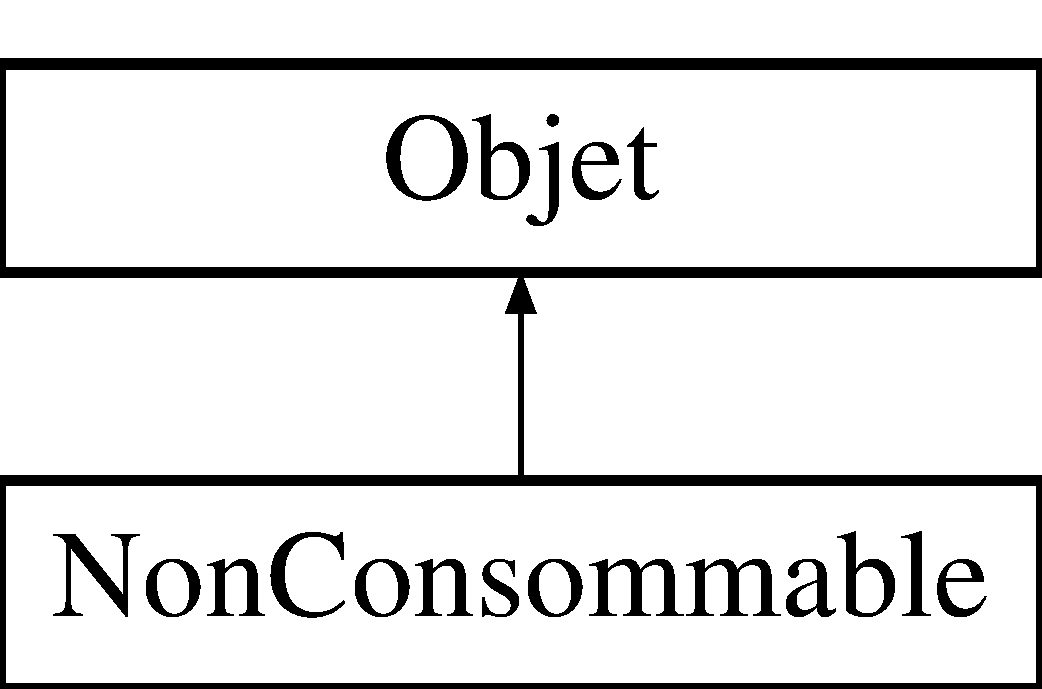
\includegraphics[height=2.000000cm]{class_non_consommable}
\end{center}
\end{figure}
\subsection*{Public Member Functions}
\begin{DoxyCompactItemize}
\item 
\hyperlink{class_non_consommable_ab2dcf94cbb47401e632a37b594ae8091}{Non\-Consommable} ()
\begin{DoxyCompactList}\small\item\em Constructeur par défaut. \end{DoxyCompactList}\item 
\hyperlink{class_non_consommable_a7c0078a9defcc714a9d6e54b97e57203}{Non\-Consommable} (int acc\-Objet, int p, string nom\-Obj, int vf, int qte\-Obj, int dur\-Vie)
\begin{DoxyCompactList}\small\item\em Constructeur de la classe nonconsommable. \end{DoxyCompactList}\item 
void \hyperlink{class_non_consommable_acf08bda31a32e15598a71bb28546629d}{setdureevie} (int new\-\_\-var)
\begin{DoxyCompactList}\small\item\em stock la valeur de la variable new\-\_\-var dans la variable dureevie. \end{DoxyCompactList}\item 
int \hyperlink{class_non_consommable_a58c576024c1daba5b28e4c243ded1c18}{getdureevie} ()
\begin{DoxyCompactList}\small\item\em Accède à la variable dureevie. \end{DoxyCompactList}\item 
void \hyperlink{class_non_consommable_acfb7cfd4a6669eaf4acb1422545ef857}{utiliser\-Objet} (\hyperlink{class_jeu}{Jeu} jeu, \hyperlink{class_heros}{Heros} $\ast$heros)
\begin{DoxyCompactList}\small\item\em Utilise un objet non consommable afin de gagner de la force. \end{DoxyCompactList}\end{DoxyCompactItemize}
\subsection*{Additional Inherited Members}


\subsection{Detailed Description}
Classe représentant les objets non consommables. 

\subsection{Constructor \& Destructor Documentation}
\hypertarget{class_non_consommable_ab2dcf94cbb47401e632a37b594ae8091}{\index{Non\-Consommable@{Non\-Consommable}!Non\-Consommable@{Non\-Consommable}}
\index{Non\-Consommable@{Non\-Consommable}!NonConsommable@{Non\-Consommable}}
\subsubsection[{Non\-Consommable}]{\setlength{\rightskip}{0pt plus 5cm}Non\-Consommable\-::\-Non\-Consommable (
\begin{DoxyParamCaption}
{}
\end{DoxyParamCaption}
)}}\label{class_non_consommable_ab2dcf94cbb47401e632a37b594ae8091}


Constructeur par défaut. 


\begin{DoxyCode}
9 \{\}
\end{DoxyCode}
\hypertarget{class_non_consommable_a7c0078a9defcc714a9d6e54b97e57203}{\index{Non\-Consommable@{Non\-Consommable}!Non\-Consommable@{Non\-Consommable}}
\index{Non\-Consommable@{Non\-Consommable}!NonConsommable@{Non\-Consommable}}
\subsubsection[{Non\-Consommable}]{\setlength{\rightskip}{0pt plus 5cm}Non\-Consommable\-::\-Non\-Consommable (
\begin{DoxyParamCaption}
\item[{int}]{acc\-Objet, }
\item[{int}]{p, }
\item[{string}]{nom\-Obj, }
\item[{int}]{vf, }
\item[{int}]{qte\-Obj, }
\item[{int}]{dur\-Vie}
\end{DoxyParamCaption}
)}}\label{class_non_consommable_a7c0078a9defcc714a9d6e54b97e57203}


Constructeur de la classe nonconsommable. 


\begin{DoxyParams}{Parameters}
{\em acc\-Objet} & L'accessibilité de l'objet à partir d'un certain âge. \\
\hline
{\em p} & Le prix de l'objet. \\
\hline
{\em nom\-Obj} & Le nom de l'objet. \\
\hline
{\em vf} & La valeur de la force que l'héros peut gagner \\
\hline
{\em qte\-Obj} & La quantité de l'objet. \\
\hline
{\em dur\-Vie} & La durée de vie de l'objet. \\
\hline
\end{DoxyParams}

\begin{DoxyCode}
11                                                                                                   : 
      \hyperlink{class_objet_aefdd826d50085897e4894ffef4597d04}{Objet}(accObjet, p, nomObj, vf, qteObj) \{
12     dureevie = durVie;\}
\end{DoxyCode}


\subsection{Member Function Documentation}
\hypertarget{class_non_consommable_a58c576024c1daba5b28e4c243ded1c18}{\index{Non\-Consommable@{Non\-Consommable}!getdureevie@{getdureevie}}
\index{getdureevie@{getdureevie}!NonConsommable@{Non\-Consommable}}
\subsubsection[{getdureevie}]{\setlength{\rightskip}{0pt plus 5cm}int Non\-Consommable\-::getdureevie (
\begin{DoxyParamCaption}
{}
\end{DoxyParamCaption}
)}}\label{class_non_consommable_a58c576024c1daba5b28e4c243ded1c18}


Accède à la variable dureevie. 

\begin{DoxyReturn}{Returns}
La durée de vie de l'objet non consommable. 
\end{DoxyReturn}

\begin{DoxyCode}
18                                        \{
19     \textcolor{keywordflow}{return} dureevie;
20   \}
\end{DoxyCode}
\hypertarget{class_non_consommable_acf08bda31a32e15598a71bb28546629d}{\index{Non\-Consommable@{Non\-Consommable}!setdureevie@{setdureevie}}
\index{setdureevie@{setdureevie}!NonConsommable@{Non\-Consommable}}
\subsubsection[{setdureevie}]{\setlength{\rightskip}{0pt plus 5cm}void Non\-Consommable\-::setdureevie (
\begin{DoxyParamCaption}
\item[{int}]{new\-\_\-var}
\end{DoxyParamCaption}
)}}\label{class_non_consommable_acf08bda31a32e15598a71bb28546629d}


stock la valeur de la variable new\-\_\-var dans la variable dureevie. 


\begin{DoxyCode}
14                                                   \{
15       dureevie = new\_var;
16   \}
\end{DoxyCode}
\hypertarget{class_non_consommable_acfb7cfd4a6669eaf4acb1422545ef857}{\index{Non\-Consommable@{Non\-Consommable}!utiliser\-Objet@{utiliser\-Objet}}
\index{utiliser\-Objet@{utiliser\-Objet}!NonConsommable@{Non\-Consommable}}
\subsubsection[{utiliser\-Objet}]{\setlength{\rightskip}{0pt plus 5cm}void Non\-Consommable\-::utiliser\-Objet (
\begin{DoxyParamCaption}
\item[{{\bf Jeu}}]{jeu, }
\item[{{\bf Heros} $\ast$}]{heros}
\end{DoxyParamCaption}
)\hspace{0.3cm}{\ttfamily [virtual]}}}\label{class_non_consommable_acfb7cfd4a6669eaf4acb1422545ef857}


Utilise un objet non consommable afin de gagner de la force. 


\begin{DoxyParams}{Parameters}
{\em jeu} & Une instance de la classe \hyperlink{class_jeu}{Jeu}. \\
\hline
{\em heros} & un pointeur sur la classe \hyperlink{class_heros}{Heros} \\
\hline
\end{DoxyParams}


Reimplemented from \hyperlink{class_objet_ab8c32a2e0b236fcf75a06a2edc1f71b6}{Objet}.


\begin{DoxyCode}
21                                                         \{
22       jeu.\hyperlink{class_jeu_aa09fb40439f16b9665a0d76679f78e4e}{afficherTexte}(\textcolor{stringliteral}{"Ce n'est pas un objet consommbale."});
23       heros->\hyperlink{class_personnage_a6745d147720906f2c85ddce11981d71f}{setForce}(heros->\hyperlink{class_personnage_a40de0ba95f25eb6f1653b6a4183763ae}{getForce}() + \hyperlink{class_objet_aa819b02977c333c0cc5e116575e951cc}{valeurForce});
24 
25 
26  \}
\end{DoxyCode}


The documentation for this class was generated from the following files\-:\begin{DoxyCompactItemize}
\item 
/nfs/usersgm/\-G\-M26/neljibbawe/\-Bureau/\-Projet\-C\-P\-P\-A\-Rendre/\-C\-P\-P R\-P\-G/\-R\-P\-G/\hyperlink{nonconsommable_8hpp}{nonconsommable.\-hpp}\item 
/nfs/usersgm/\-G\-M26/neljibbawe/\-Bureau/\-Projet\-C\-P\-P\-A\-Rendre/\-C\-P\-P R\-P\-G/\-R\-P\-G/\hyperlink{nonconsommable_8cpp}{nonconsommable.\-cpp}\end{DoxyCompactItemize}

\hypertarget{class_objet}{\section{Objet Class Reference}
\label{class_objet}\index{Objet@{Objet}}
}


Classe représentant les objets.  




{\ttfamily \#include $<$objet.\-hpp$>$}

Inheritance diagram for Objet\-:\begin{figure}[H]
\begin{center}
\leavevmode
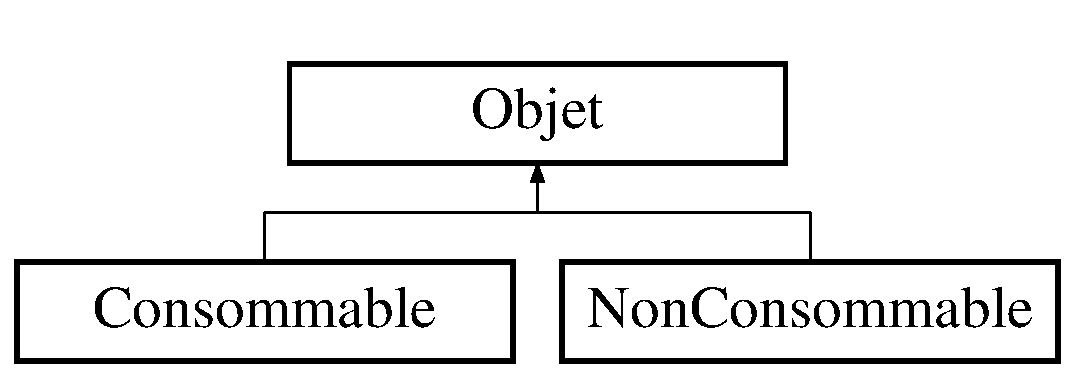
\includegraphics[height=2.000000cm]{class_objet}
\end{center}
\end{figure}
\subsection*{Public Member Functions}
\begin{DoxyCompactItemize}
\item 
\hyperlink{class_objet_aefdd826d50085897e4894ffef4597d04}{Objet} ()
\begin{DoxyCompactList}\small\item\em Constructeur par défaut. \end{DoxyCompactList}\item 
\hyperlink{class_objet_a6fb1713f353f5ede79c339874be7c29b}{Objet} (int acc\-Objet, int p, string nom\-Obj, int vf, int qte\-Obj)
\begin{DoxyCompactList}\small\item\em Constructeur de la classe objet. \end{DoxyCompactList}\item 
void \hyperlink{class_objet_a63d919b38358563e308c8fa4a6d1d1e8}{set\-Nom\-Objet} (string new\-\_\-var)
\begin{DoxyCompactList}\small\item\em stock la valeur de la variable new\-\_\-var dans la variable nom\-Objet. \end{DoxyCompactList}\item 
string \hyperlink{class_objet_a843e99ecd1e150589f8db23f43dd27b0}{get\-Nom\-Objet} ()
\begin{DoxyCompactList}\small\item\em Accède à la variable nom\-Objet. \end{DoxyCompactList}\item 
void \hyperlink{class_objet_a3b4253aca64e7fa3fb1303449579f3be}{set\-Prix} (int new\-\_\-var)
\begin{DoxyCompactList}\small\item\em stock la valeur de la variable new\-\_\-var dans la variable prix. \end{DoxyCompactList}\item 
int \hyperlink{class_objet_a9b36c37091e821bc8f00d6bfd3665a66}{get\-Prix} ()
\begin{DoxyCompactList}\small\item\em Accède à la variable prix. \end{DoxyCompactList}\item 
void \hyperlink{class_objet_a46ff6cb720f950f6a9cc607427ae98cc}{set\-Valeur\-Force} (int new\-\_\-var)
\begin{DoxyCompactList}\small\item\em stock la valeur de la variable new\-\_\-var dans la variable valeur\-Force. \end{DoxyCompactList}\item 
int \hyperlink{class_objet_af57c602bd00d1478cfefb8d568bad309}{get\-Valeur\-Force} ()
\begin{DoxyCompactList}\small\item\em Accède à la variable valeur\-Force. \end{DoxyCompactList}\item 
void \hyperlink{class_objet_a867e1cec21732464c50251d8b5abb00e}{set\-Access\-Objet} (int var)
\begin{DoxyCompactList}\small\item\em stock la valeur de la variable var dans la variable access\-Objet. \end{DoxyCompactList}\item 
int \hyperlink{class_objet_a89e96aceca5fa4ff383bec982be3e39a}{get\-Access\-Objet} ()
\begin{DoxyCompactList}\small\item\em Accède à la variable access\-Objet. \end{DoxyCompactList}\item 
void \hyperlink{class_objet_a667447b583f58e06a0ac8407d2fed45a}{set\-Quantite\-Objet} (int var)
\begin{DoxyCompactList}\small\item\em stock la valeur de la variable var dans la variable quantite\-Objet. \end{DoxyCompactList}\item 
int \hyperlink{class_objet_a48ed4b5205b42401520102586cfe2265}{get\-Quantite\-Objet} ()
\begin{DoxyCompactList}\small\item\em Accède à la variable quantite\-Objet. \end{DoxyCompactList}\item 
void \hyperlink{class_objet_a812fd7438f15ff8f5b530187affc3cc9}{initialiser\-Objet} ()
\begin{DoxyCompactList}\small\item\em Initialise l'objet. \end{DoxyCompactList}\item 
virtual void \hyperlink{class_objet_ab8c32a2e0b236fcf75a06a2edc1f71b6}{utiliser\-Objet} (\hyperlink{class_jeu}{Jeu} jeu, \hyperlink{class_heros}{Heros} $\ast$heros)
\begin{DoxyCompactList}\small\item\em sert à utiliser un objet. C'est une méthode virtuelle qui va être redéfinie dans chacune des classes filles de \hyperlink{class_objet}{Objet}. \end{DoxyCompactList}\end{DoxyCompactItemize}
\subsection*{Protected Attributes}
\begin{DoxyCompactItemize}
\item 
int \hyperlink{class_objet_a420bad3c2d47108539b1d93156966924}{access\-Objet}
\begin{DoxyCompactList}\small\item\em L'âge à partir duquel on peut accèder à l'objet. \end{DoxyCompactList}\item 
string \hyperlink{class_objet_aeae2038324beeebfdd3ef7f793ca0b21}{nom\-Objet}
\begin{DoxyCompactList}\small\item\em Le nom de l'objet. \end{DoxyCompactList}\item 
int \hyperlink{class_objet_abdcebe17a8c444c7e3c982d5d99930cd}{prix}
\begin{DoxyCompactList}\small\item\em Le prix de l'objet. \end{DoxyCompactList}\item 
int \hyperlink{class_objet_aa819b02977c333c0cc5e116575e951cc}{valeur\-Force}
\begin{DoxyCompactList}\small\item\em La valeur de la force que l'objet permet de gagner. \end{DoxyCompactList}\item 
int \hyperlink{class_objet_a97d1fa595a507f7c06f241d73c63bb94}{quantite\-Objet}
\begin{DoxyCompactList}\small\item\em La qunatité de l'objet. \end{DoxyCompactList}\end{DoxyCompactItemize}


\subsection{Detailed Description}
Classe représentant les objets. 

\subsection{Constructor \& Destructor Documentation}
\hypertarget{class_objet_aefdd826d50085897e4894ffef4597d04}{\index{Objet@{Objet}!Objet@{Objet}}
\index{Objet@{Objet}!Objet@{Objet}}
\subsubsection[{Objet}]{\setlength{\rightskip}{0pt plus 5cm}Objet\-::\-Objet (
\begin{DoxyParamCaption}
{}
\end{DoxyParamCaption}
)}}\label{class_objet_aefdd826d50085897e4894ffef4597d04}


Constructeur par défaut. 


\begin{DoxyCode}
18             \{
19     \}
\end{DoxyCode}
\hypertarget{class_objet_a6fb1713f353f5ede79c339874be7c29b}{\index{Objet@{Objet}!Objet@{Objet}}
\index{Objet@{Objet}!Objet@{Objet}}
\subsubsection[{Objet}]{\setlength{\rightskip}{0pt plus 5cm}Objet\-::\-Objet (
\begin{DoxyParamCaption}
\item[{int}]{acc\-Objet, }
\item[{int}]{p, }
\item[{string}]{nom\-Obj, }
\item[{int}]{vf, }
\item[{int}]{qte\-Obj}
\end{DoxyParamCaption}
)}}\label{class_objet_a6fb1713f353f5ede79c339874be7c29b}


Constructeur de la classe objet. 


\begin{DoxyParams}{Parameters}
{\em acc\-Objet} & L'accessibilité de l'objet à partir d'un certain âge. \\
\hline
{\em p} & Le prix de l'objet. \\
\hline
{\em nom\-Obj} & Le nom de l'objet. \\
\hline
{\em vf} & La valeur de la force que l'héros peut gagner. \\
\hline
{\em qte\-Obj} & La quantité de l'objet. \\
\hline
\end{DoxyParams}

\begin{DoxyCode}
11                                                                   \{
12     \hyperlink{class_objet_a420bad3c2d47108539b1d93156966924}{accessObjet} = accObjet;
13     \hyperlink{class_objet_aeae2038324beeebfdd3ef7f793ca0b21}{nomObjet} = nomObj;
14     \hyperlink{class_objet_abdcebe17a8c444c7e3c982d5d99930cd}{prix} = p;
15     \hyperlink{class_objet_aa819b02977c333c0cc5e116575e951cc}{valeurForce} = vf;
16     \hyperlink{class_objet_a97d1fa595a507f7c06f241d73c63bb94}{quantiteObjet} = qteObj;
17 \}
\end{DoxyCode}


\subsection{Member Function Documentation}
\hypertarget{class_objet_a89e96aceca5fa4ff383bec982be3e39a}{\index{Objet@{Objet}!get\-Access\-Objet@{get\-Access\-Objet}}
\index{get\-Access\-Objet@{get\-Access\-Objet}!Objet@{Objet}}
\subsubsection[{get\-Access\-Objet}]{\setlength{\rightskip}{0pt plus 5cm}int Objet\-::get\-Access\-Objet (
\begin{DoxyParamCaption}
{}
\end{DoxyParamCaption}
)}}\label{class_objet_a89e96aceca5fa4ff383bec982be3e39a}


Accède à la variable access\-Objet. 

\begin{DoxyReturn}{Returns}
L'âge à partir duquel l'objet sera accessible. 
\end{DoxyReturn}

\begin{DoxyCode}
49                             \{
50     \textcolor{keywordflow}{return} \hyperlink{class_objet_a420bad3c2d47108539b1d93156966924}{accessObjet};
51   \}
\end{DoxyCode}
\hypertarget{class_objet_a843e99ecd1e150589f8db23f43dd27b0}{\index{Objet@{Objet}!get\-Nom\-Objet@{get\-Nom\-Objet}}
\index{get\-Nom\-Objet@{get\-Nom\-Objet}!Objet@{Objet}}
\subsubsection[{get\-Nom\-Objet}]{\setlength{\rightskip}{0pt plus 5cm}string Objet\-::get\-Nom\-Objet (
\begin{DoxyParamCaption}
{}
\end{DoxyParamCaption}
)}}\label{class_objet_a843e99ecd1e150589f8db23f43dd27b0}


Accède à la variable nom\-Objet. 

\begin{DoxyReturn}{Returns}
Le nom de l'objet. 
\end{DoxyReturn}

\begin{DoxyCode}
25                                \{
26     \textcolor{keywordflow}{return} \hyperlink{class_objet_aeae2038324beeebfdd3ef7f793ca0b21}{nomObjet};
27   \}
\end{DoxyCode}
\hypertarget{class_objet_a9b36c37091e821bc8f00d6bfd3665a66}{\index{Objet@{Objet}!get\-Prix@{get\-Prix}}
\index{get\-Prix@{get\-Prix}!Objet@{Objet}}
\subsubsection[{get\-Prix}]{\setlength{\rightskip}{0pt plus 5cm}int Objet\-::get\-Prix (
\begin{DoxyParamCaption}
{}
\end{DoxyParamCaption}
)}}\label{class_objet_a9b36c37091e821bc8f00d6bfd3665a66}


Accède à la variable prix. 

\begin{DoxyReturn}{Returns}
Le prix de l'objet. 
\end{DoxyReturn}

\begin{DoxyCode}
33                          \{
34     \textcolor{keywordflow}{return} \hyperlink{class_objet_abdcebe17a8c444c7e3c982d5d99930cd}{prix};
35   \}
\end{DoxyCode}
\hypertarget{class_objet_a48ed4b5205b42401520102586cfe2265}{\index{Objet@{Objet}!get\-Quantite\-Objet@{get\-Quantite\-Objet}}
\index{get\-Quantite\-Objet@{get\-Quantite\-Objet}!Objet@{Objet}}
\subsubsection[{get\-Quantite\-Objet}]{\setlength{\rightskip}{0pt plus 5cm}int Objet\-::get\-Quantite\-Objet (
\begin{DoxyParamCaption}
{}
\end{DoxyParamCaption}
)}}\label{class_objet_a48ed4b5205b42401520102586cfe2265}


Accède à la variable quantite\-Objet. 

\begin{DoxyReturn}{Returns}
La quantité de l'objet. 
\end{DoxyReturn}

\begin{DoxyCode}
57                               \{
58     \textcolor{keywordflow}{return} \hyperlink{class_objet_a97d1fa595a507f7c06f241d73c63bb94}{quantiteObjet};
59   \}
\end{DoxyCode}
\hypertarget{class_objet_af57c602bd00d1478cfefb8d568bad309}{\index{Objet@{Objet}!get\-Valeur\-Force@{get\-Valeur\-Force}}
\index{get\-Valeur\-Force@{get\-Valeur\-Force}!Objet@{Objet}}
\subsubsection[{get\-Valeur\-Force}]{\setlength{\rightskip}{0pt plus 5cm}int Objet\-::get\-Valeur\-Force (
\begin{DoxyParamCaption}
{}
\end{DoxyParamCaption}
)}}\label{class_objet_af57c602bd00d1478cfefb8d568bad309}


Accède à la variable valeur\-Force. 

\begin{DoxyReturn}{Returns}
La valeur de la force que l'héros peut gagner. 
\end{DoxyReturn}

\begin{DoxyCode}
41                                 \{
42     \textcolor{keywordflow}{return} \hyperlink{class_objet_aa819b02977c333c0cc5e116575e951cc}{valeurForce};
43   \}
\end{DoxyCode}
\hypertarget{class_objet_a812fd7438f15ff8f5b530187affc3cc9}{\index{Objet@{Objet}!initialiser\-Objet@{initialiser\-Objet}}
\index{initialiser\-Objet@{initialiser\-Objet}!Objet@{Objet}}
\subsubsection[{initialiser\-Objet}]{\setlength{\rightskip}{0pt plus 5cm}void Objet\-::initialiser\-Objet (
\begin{DoxyParamCaption}
{}
\end{DoxyParamCaption}
)}}\label{class_objet_a812fd7438f15ff8f5b530187affc3cc9}


Initialise l'objet. 

\hypertarget{class_objet_a867e1cec21732464c50251d8b5abb00e}{\index{Objet@{Objet}!set\-Access\-Objet@{set\-Access\-Objet}}
\index{set\-Access\-Objet@{set\-Access\-Objet}!Objet@{Objet}}
\subsubsection[{set\-Access\-Objet}]{\setlength{\rightskip}{0pt plus 5cm}void Objet\-::set\-Access\-Objet (
\begin{DoxyParamCaption}
\item[{int}]{var}
\end{DoxyParamCaption}
)}}\label{class_objet_a867e1cec21732464c50251d8b5abb00e}


stock la valeur de la variable var dans la variable access\-Objet. 


\begin{DoxyCode}
45                                    \{
46     \hyperlink{class_objet_a420bad3c2d47108539b1d93156966924}{accessObjet} =var;
47   \}
\end{DoxyCode}
\hypertarget{class_objet_a63d919b38358563e308c8fa4a6d1d1e8}{\index{Objet@{Objet}!set\-Nom\-Objet@{set\-Nom\-Objet}}
\index{set\-Nom\-Objet@{set\-Nom\-Objet}!Objet@{Objet}}
\subsubsection[{set\-Nom\-Objet}]{\setlength{\rightskip}{0pt plus 5cm}void Objet\-::set\-Nom\-Objet (
\begin{DoxyParamCaption}
\item[{string}]{new\-\_\-var}
\end{DoxyParamCaption}
)}}\label{class_objet_a63d919b38358563e308c8fa4a6d1d1e8}


stock la valeur de la variable new\-\_\-var dans la variable nom\-Objet. 


\begin{DoxyCode}
21                                            \{
22       \hyperlink{class_objet_aeae2038324beeebfdd3ef7f793ca0b21}{nomObjet} = new\_var;
23   \}
\end{DoxyCode}
\hypertarget{class_objet_a3b4253aca64e7fa3fb1303449579f3be}{\index{Objet@{Objet}!set\-Prix@{set\-Prix}}
\index{set\-Prix@{set\-Prix}!Objet@{Objet}}
\subsubsection[{set\-Prix}]{\setlength{\rightskip}{0pt plus 5cm}void Objet\-::set\-Prix (
\begin{DoxyParamCaption}
\item[{int}]{new\-\_\-var}
\end{DoxyParamCaption}
)}}\label{class_objet_a3b4253aca64e7fa3fb1303449579f3be}


stock la valeur de la variable new\-\_\-var dans la variable prix. 


\begin{DoxyCode}
29                                      \{
30       \hyperlink{class_objet_abdcebe17a8c444c7e3c982d5d99930cd}{prix} = new\_var;
31   \}
\end{DoxyCode}
\hypertarget{class_objet_a667447b583f58e06a0ac8407d2fed45a}{\index{Objet@{Objet}!set\-Quantite\-Objet@{set\-Quantite\-Objet}}
\index{set\-Quantite\-Objet@{set\-Quantite\-Objet}!Objet@{Objet}}
\subsubsection[{set\-Quantite\-Objet}]{\setlength{\rightskip}{0pt plus 5cm}void Objet\-::set\-Quantite\-Objet (
\begin{DoxyParamCaption}
\item[{int}]{var}
\end{DoxyParamCaption}
)}}\label{class_objet_a667447b583f58e06a0ac8407d2fed45a}


stock la valeur de la variable var dans la variable quantite\-Objet. 


\begin{DoxyCode}
53                                       \{
54     \hyperlink{class_objet_a97d1fa595a507f7c06f241d73c63bb94}{quantiteObjet} = var;
55   \}
\end{DoxyCode}
\hypertarget{class_objet_a46ff6cb720f950f6a9cc607427ae98cc}{\index{Objet@{Objet}!set\-Valeur\-Force@{set\-Valeur\-Force}}
\index{set\-Valeur\-Force@{set\-Valeur\-Force}!Objet@{Objet}}
\subsubsection[{set\-Valeur\-Force}]{\setlength{\rightskip}{0pt plus 5cm}void Objet\-::set\-Valeur\-Force (
\begin{DoxyParamCaption}
\item[{int}]{new\-\_\-var}
\end{DoxyParamCaption}
)}}\label{class_objet_a46ff6cb720f950f6a9cc607427ae98cc}


stock la valeur de la variable new\-\_\-var dans la variable valeur\-Force. 


\begin{DoxyCode}
37                                             \{
38       \hyperlink{class_objet_aa819b02977c333c0cc5e116575e951cc}{valeurForce} = new\_var;
39   \}
\end{DoxyCode}
\hypertarget{class_objet_ab8c32a2e0b236fcf75a06a2edc1f71b6}{\index{Objet@{Objet}!utiliser\-Objet@{utiliser\-Objet}}
\index{utiliser\-Objet@{utiliser\-Objet}!Objet@{Objet}}
\subsubsection[{utiliser\-Objet}]{\setlength{\rightskip}{0pt plus 5cm}void Objet\-::utiliser\-Objet (
\begin{DoxyParamCaption}
\item[{{\bf Jeu}}]{jeu, }
\item[{{\bf Heros} $\ast$}]{heros}
\end{DoxyParamCaption}
)\hspace{0.3cm}{\ttfamily [virtual]}}}\label{class_objet_ab8c32a2e0b236fcf75a06a2edc1f71b6}


sert à utiliser un objet. C'est une méthode virtuelle qui va être redéfinie dans chacune des classes filles de \hyperlink{class_objet}{Objet}. 


\begin{DoxyParams}{Parameters}
{\em jeu} & Une instance de la classe \hyperlink{class_jeu}{Jeu}. \\
\hline
{\em heros} & un pointeur sur la classe \hyperlink{class_heros}{Heros}. \\
\hline
\end{DoxyParams}


Reimplemented in \hyperlink{class_consommable_ab2105902385a78cbca8496fdde262d2f}{Consommable}, and \hyperlink{class_non_consommable_acfb7cfd4a6669eaf4acb1422545ef857}{Non\-Consommable}.


\begin{DoxyCode}
64                                                   \{
65 \}
\end{DoxyCode}


\subsection{Member Data Documentation}
\hypertarget{class_objet_a420bad3c2d47108539b1d93156966924}{\index{Objet@{Objet}!access\-Objet@{access\-Objet}}
\index{access\-Objet@{access\-Objet}!Objet@{Objet}}
\subsubsection[{access\-Objet}]{\setlength{\rightskip}{0pt plus 5cm}int Objet\-::access\-Objet\hspace{0.3cm}{\ttfamily [protected]}}}\label{class_objet_a420bad3c2d47108539b1d93156966924}


L'âge à partir duquel on peut accèder à l'objet. 

\hypertarget{class_objet_aeae2038324beeebfdd3ef7f793ca0b21}{\index{Objet@{Objet}!nom\-Objet@{nom\-Objet}}
\index{nom\-Objet@{nom\-Objet}!Objet@{Objet}}
\subsubsection[{nom\-Objet}]{\setlength{\rightskip}{0pt plus 5cm}string Objet\-::nom\-Objet\hspace{0.3cm}{\ttfamily [protected]}}}\label{class_objet_aeae2038324beeebfdd3ef7f793ca0b21}


Le nom de l'objet. 

\hypertarget{class_objet_abdcebe17a8c444c7e3c982d5d99930cd}{\index{Objet@{Objet}!prix@{prix}}
\index{prix@{prix}!Objet@{Objet}}
\subsubsection[{prix}]{\setlength{\rightskip}{0pt plus 5cm}int Objet\-::prix\hspace{0.3cm}{\ttfamily [protected]}}}\label{class_objet_abdcebe17a8c444c7e3c982d5d99930cd}


Le prix de l'objet. 

\hypertarget{class_objet_a97d1fa595a507f7c06f241d73c63bb94}{\index{Objet@{Objet}!quantite\-Objet@{quantite\-Objet}}
\index{quantite\-Objet@{quantite\-Objet}!Objet@{Objet}}
\subsubsection[{quantite\-Objet}]{\setlength{\rightskip}{0pt plus 5cm}int Objet\-::quantite\-Objet\hspace{0.3cm}{\ttfamily [protected]}}}\label{class_objet_a97d1fa595a507f7c06f241d73c63bb94}


La qunatité de l'objet. 

\hypertarget{class_objet_aa819b02977c333c0cc5e116575e951cc}{\index{Objet@{Objet}!valeur\-Force@{valeur\-Force}}
\index{valeur\-Force@{valeur\-Force}!Objet@{Objet}}
\subsubsection[{valeur\-Force}]{\setlength{\rightskip}{0pt plus 5cm}int Objet\-::valeur\-Force\hspace{0.3cm}{\ttfamily [protected]}}}\label{class_objet_aa819b02977c333c0cc5e116575e951cc}


La valeur de la force que l'objet permet de gagner. 



The documentation for this class was generated from the following files\-:\begin{DoxyCompactItemize}
\item 
/nfs/usersgm/\-G\-M26/neljibbawe/\-Bureau/\-Projet\-C\-P\-P\-A\-Rendre/\-C\-P\-P R\-P\-G/\-R\-P\-G/\hyperlink{objet_8hpp}{objet.\-hpp}\item 
/nfs/usersgm/\-G\-M26/neljibbawe/\-Bureau/\-Projet\-C\-P\-P\-A\-Rendre/\-C\-P\-P R\-P\-G/\-R\-P\-G/\hyperlink{objet_8cpp}{objet.\-cpp}\end{DoxyCompactItemize}

\hypertarget{class_personnage}{\section{Personnage Class Reference}
\label{class_personnage}\index{Personnage@{Personnage}}
}


Classe représentant les personnages.  




{\ttfamily \#include $<$personnage.\-hpp$>$}

Inheritance diagram for Personnage\-:\begin{figure}[H]
\begin{center}
\leavevmode
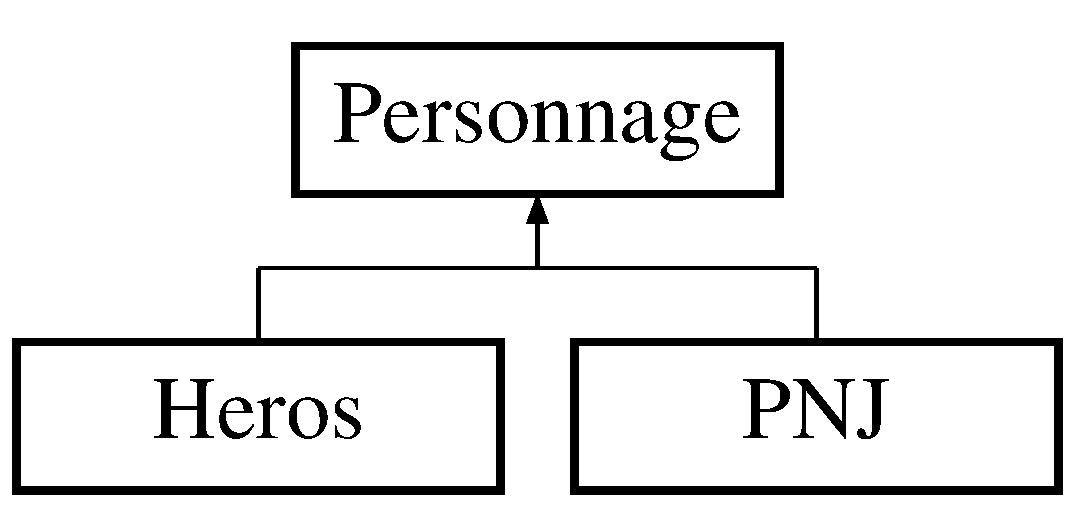
\includegraphics[height=2.000000cm]{class_personnage}
\end{center}
\end{figure}
\subsection*{Public Member Functions}
\begin{DoxyCompactItemize}
\item 
\hyperlink{class_personnage_abec36eb0310adc71f3375297fc590c65}{Personnage} ()
\begin{DoxyCompactList}\small\item\em Constructeur par défaut. \end{DoxyCompactList}\item 
\hyperlink{class_personnage_aee7b1cf6fb3ae9c6dd9d834fb9a7557c}{Personnage} (int intelp, int forcep, int agep, string nomp)
\begin{DoxyCompactList}\small\item\em Constructeur de la classe personnage. \end{DoxyCompactList}\item 
void \hyperlink{class_personnage_af8b3c4f6c0f7035678d9ecf574976650}{set\-Intelligence} (int new\-\_\-var)
\begin{DoxyCompactList}\small\item\em stock la valeur de la variable new\-\_\-var dans la variable Intelligence. \end{DoxyCompactList}\item 
int \hyperlink{class_personnage_a250eec1aba0df7a105dd564e4cd02b0b}{get\-Intelligence} ()
\begin{DoxyCompactList}\small\item\em Accède à la variable Intelligence. \end{DoxyCompactList}\item 
void \hyperlink{class_personnage_a6745d147720906f2c85ddce11981d71f}{set\-Force} (int new\-\_\-var)
\begin{DoxyCompactList}\small\item\em stock la valeur de la variable new\-\_\-var dans la variable Force. \end{DoxyCompactList}\item 
int \hyperlink{class_personnage_a40de0ba95f25eb6f1653b6a4183763ae}{get\-Force} ()
\begin{DoxyCompactList}\small\item\em Accède à la variable Force. \end{DoxyCompactList}\item 
void \hyperlink{class_personnage_a5d9ef278febb61a54c8d61e9eff79aa4}{set\-Age} (int new\-\_\-var)
\begin{DoxyCompactList}\small\item\em stock la valeur de la variable new\-\_\-var dans la variable Age. \end{DoxyCompactList}\item 
int \hyperlink{class_personnage_a991d7e1cf4662e245ad72e76b9eb9d53}{get\-Age} ()
\begin{DoxyCompactList}\small\item\em Accède à la variable Age. \end{DoxyCompactList}\item 
void \hyperlink{class_personnage_a5071fd1a8c64b3b2653681b8a867405d}{set\-Nom} (string var)
\begin{DoxyCompactList}\small\item\em stock la valeur de la variable var dans la variable Nom. \end{DoxyCompactList}\item 
string \hyperlink{class_personnage_a519301399a9bee1557858aa50a04a85a}{get\-Nom} ()
\begin{DoxyCompactList}\small\item\em Accède à la variable Nom. \end{DoxyCompactList}\end{DoxyCompactItemize}
\subsection*{Protected Attributes}
\begin{DoxyCompactItemize}
\item 
int \hyperlink{class_personnage_a8e9bc213349fb0553d76d4da6a711231}{intelligence}
\begin{DoxyCompactList}\small\item\em La valeur de l'intelligence du personnage. \end{DoxyCompactList}\item 
int \hyperlink{class_personnage_a823cd88582efee2ea29d199f96dcc677}{force}
\begin{DoxyCompactList}\small\item\em La valeur de la force du personnage. \end{DoxyCompactList}\item 
int \hyperlink{class_personnage_a2aa943e3c255f221eb9e57e8d134641f}{age}
\begin{DoxyCompactList}\small\item\em L'âge du personnage. \end{DoxyCompactList}\item 
string \hyperlink{class_personnage_acb7331b96dfc9f2aec78c60799030302}{nom}
\begin{DoxyCompactList}\small\item\em Le nom du personnage. \end{DoxyCompactList}\end{DoxyCompactItemize}


\subsection{Detailed Description}
Classe représentant les personnages. 

\subsection{Constructor \& Destructor Documentation}
\hypertarget{class_personnage_abec36eb0310adc71f3375297fc590c65}{\index{Personnage@{Personnage}!Personnage@{Personnage}}
\index{Personnage@{Personnage}!Personnage@{Personnage}}
\subsubsection[{Personnage}]{\setlength{\rightskip}{0pt plus 5cm}Personnage\-::\-Personnage (
\begin{DoxyParamCaption}
{}
\end{DoxyParamCaption}
)}}\label{class_personnage_abec36eb0310adc71f3375297fc590c65}


Constructeur par défaut. 


\begin{DoxyCode}
7 \{\}
\end{DoxyCode}
\hypertarget{class_personnage_aee7b1cf6fb3ae9c6dd9d834fb9a7557c}{\index{Personnage@{Personnage}!Personnage@{Personnage}}
\index{Personnage@{Personnage}!Personnage@{Personnage}}
\subsubsection[{Personnage}]{\setlength{\rightskip}{0pt plus 5cm}Personnage\-::\-Personnage (
\begin{DoxyParamCaption}
\item[{int}]{intelp, }
\item[{int}]{forcep, }
\item[{int}]{agep, }
\item[{string}]{nomp}
\end{DoxyParamCaption}
)}}\label{class_personnage_aee7b1cf6fb3ae9c6dd9d834fb9a7557c}


Constructeur de la classe personnage. 


\begin{DoxyParams}{Parameters}
{\em intelp} & La valeur de l'intelligence du personnage. \\
\hline
{\em forcep} & La valeur de la force du personnage. \\
\hline
{\em agep} & L'âge du personnage. \\
\hline
{\em nomp} & le nom du personnage. \\
\hline
\end{DoxyParams}

\begin{DoxyCode}
9                                                                    \{
10     \hyperlink{class_personnage_a8e9bc213349fb0553d76d4da6a711231}{intelligence} = intelp;
11     \hyperlink{class_personnage_a823cd88582efee2ea29d199f96dcc677}{force} = forcep;
12     \hyperlink{class_personnage_a2aa943e3c255f221eb9e57e8d134641f}{age} = agep;
13     \hyperlink{class_personnage_acb7331b96dfc9f2aec78c60799030302}{nom} = nomp;
14     \}
\end{DoxyCode}


\subsection{Member Function Documentation}
\hypertarget{class_personnage_a991d7e1cf4662e245ad72e76b9eb9d53}{\index{Personnage@{Personnage}!get\-Age@{get\-Age}}
\index{get\-Age@{get\-Age}!Personnage@{Personnage}}
\subsubsection[{get\-Age}]{\setlength{\rightskip}{0pt plus 5cm}int Personnage\-::get\-Age (
\begin{DoxyParamCaption}
{}
\end{DoxyParamCaption}
)}}\label{class_personnage_a991d7e1cf4662e245ad72e76b9eb9d53}


Accède à la variable Age. 

\begin{DoxyReturn}{Returns}
La valeur de l'âge. 
\end{DoxyReturn}

\begin{DoxyCode}
41                             \{
42     \textcolor{keywordflow}{return} \hyperlink{class_personnage_a2aa943e3c255f221eb9e57e8d134641f}{age};
43   \}
\end{DoxyCode}
\hypertarget{class_personnage_a40de0ba95f25eb6f1653b6a4183763ae}{\index{Personnage@{Personnage}!get\-Force@{get\-Force}}
\index{get\-Force@{get\-Force}!Personnage@{Personnage}}
\subsubsection[{get\-Force}]{\setlength{\rightskip}{0pt plus 5cm}int Personnage\-::get\-Force (
\begin{DoxyParamCaption}
{}
\end{DoxyParamCaption}
)}}\label{class_personnage_a40de0ba95f25eb6f1653b6a4183763ae}


Accède à la variable Force. 

\begin{DoxyReturn}{Returns}
La valeur de la force. 
\end{DoxyReturn}

\begin{DoxyCode}
33                               \{
34     \textcolor{keywordflow}{return} \hyperlink{class_personnage_a823cd88582efee2ea29d199f96dcc677}{force};
35   \}
\end{DoxyCode}
\hypertarget{class_personnage_a250eec1aba0df7a105dd564e4cd02b0b}{\index{Personnage@{Personnage}!get\-Intelligence@{get\-Intelligence}}
\index{get\-Intelligence@{get\-Intelligence}!Personnage@{Personnage}}
\subsubsection[{get\-Intelligence}]{\setlength{\rightskip}{0pt plus 5cm}int Personnage\-::get\-Intelligence (
\begin{DoxyParamCaption}
{}
\end{DoxyParamCaption}
)}}\label{class_personnage_a250eec1aba0df7a105dd564e4cd02b0b}


Accède à la variable Intelligence. 

\begin{DoxyReturn}{Returns}
La valeur de l'intelligence. 
\end{DoxyReturn}

\begin{DoxyCode}
25                                      \{
26     \textcolor{keywordflow}{return} \hyperlink{class_personnage_a8e9bc213349fb0553d76d4da6a711231}{intelligence};
27   \}
\end{DoxyCode}
\hypertarget{class_personnage_a519301399a9bee1557858aa50a04a85a}{\index{Personnage@{Personnage}!get\-Nom@{get\-Nom}}
\index{get\-Nom@{get\-Nom}!Personnage@{Personnage}}
\subsubsection[{get\-Nom}]{\setlength{\rightskip}{0pt plus 5cm}string Personnage\-::get\-Nom (
\begin{DoxyParamCaption}
{}
\end{DoxyParamCaption}
)}}\label{class_personnage_a519301399a9bee1557858aa50a04a85a}


Accède à la variable Nom. 

\begin{DoxyReturn}{Returns}
Le nom. 
\end{DoxyReturn}

\begin{DoxyCode}
18                           \{
19     \textcolor{keywordflow}{return} \hyperlink{class_personnage_acb7331b96dfc9f2aec78c60799030302}{nom};
20 \}
\end{DoxyCode}
\hypertarget{class_personnage_a5d9ef278febb61a54c8d61e9eff79aa4}{\index{Personnage@{Personnage}!set\-Age@{set\-Age}}
\index{set\-Age@{set\-Age}!Personnage@{Personnage}}
\subsubsection[{set\-Age}]{\setlength{\rightskip}{0pt plus 5cm}void Personnage\-::set\-Age (
\begin{DoxyParamCaption}
\item[{int}]{new\-\_\-var}
\end{DoxyParamCaption}
)}}\label{class_personnage_a5d9ef278febb61a54c8d61e9eff79aa4}


stock la valeur de la variable new\-\_\-var dans la variable Age. 


\begin{DoxyCode}
37                                         \{
38       \hyperlink{class_personnage_a2aa943e3c255f221eb9e57e8d134641f}{age} = new\_var;
39   \}
\end{DoxyCode}
\hypertarget{class_personnage_a6745d147720906f2c85ddce11981d71f}{\index{Personnage@{Personnage}!set\-Force@{set\-Force}}
\index{set\-Force@{set\-Force}!Personnage@{Personnage}}
\subsubsection[{set\-Force}]{\setlength{\rightskip}{0pt plus 5cm}void Personnage\-::set\-Force (
\begin{DoxyParamCaption}
\item[{int}]{new\-\_\-var}
\end{DoxyParamCaption}
)}}\label{class_personnage_a6745d147720906f2c85ddce11981d71f}


stock la valeur de la variable new\-\_\-var dans la variable Force. 


\begin{DoxyCode}
29                                           \{
30       \hyperlink{class_personnage_a823cd88582efee2ea29d199f96dcc677}{force} = new\_var;
31   \}
\end{DoxyCode}
\hypertarget{class_personnage_af8b3c4f6c0f7035678d9ecf574976650}{\index{Personnage@{Personnage}!set\-Intelligence@{set\-Intelligence}}
\index{set\-Intelligence@{set\-Intelligence}!Personnage@{Personnage}}
\subsubsection[{set\-Intelligence}]{\setlength{\rightskip}{0pt plus 5cm}void Personnage\-::set\-Intelligence (
\begin{DoxyParamCaption}
\item[{int}]{new\-\_\-var}
\end{DoxyParamCaption}
)}}\label{class_personnage_af8b3c4f6c0f7035678d9ecf574976650}


stock la valeur de la variable new\-\_\-var dans la variable Intelligence. 


\begin{DoxyCode}
21                                                  \{
22       \hyperlink{class_personnage_a8e9bc213349fb0553d76d4da6a711231}{intelligence} = new\_var;
23   \}
\end{DoxyCode}
\hypertarget{class_personnage_a5071fd1a8c64b3b2653681b8a867405d}{\index{Personnage@{Personnage}!set\-Nom@{set\-Nom}}
\index{set\-Nom@{set\-Nom}!Personnage@{Personnage}}
\subsubsection[{set\-Nom}]{\setlength{\rightskip}{0pt plus 5cm}void Personnage\-::set\-Nom (
\begin{DoxyParamCaption}
\item[{string}]{var}
\end{DoxyParamCaption}
)}}\label{class_personnage_a5071fd1a8c64b3b2653681b8a867405d}


stock la valeur de la variable var dans la variable Nom. 


\begin{DoxyCode}
15                                    \{
16     \hyperlink{class_personnage_acb7331b96dfc9f2aec78c60799030302}{nom} = var;
17 \}
\end{DoxyCode}


\subsection{Member Data Documentation}
\hypertarget{class_personnage_a2aa943e3c255f221eb9e57e8d134641f}{\index{Personnage@{Personnage}!age@{age}}
\index{age@{age}!Personnage@{Personnage}}
\subsubsection[{age}]{\setlength{\rightskip}{0pt plus 5cm}int Personnage\-::age\hspace{0.3cm}{\ttfamily [protected]}}}\label{class_personnage_a2aa943e3c255f221eb9e57e8d134641f}


L'âge du personnage. 

\hypertarget{class_personnage_a823cd88582efee2ea29d199f96dcc677}{\index{Personnage@{Personnage}!force@{force}}
\index{force@{force}!Personnage@{Personnage}}
\subsubsection[{force}]{\setlength{\rightskip}{0pt plus 5cm}int Personnage\-::force\hspace{0.3cm}{\ttfamily [protected]}}}\label{class_personnage_a823cd88582efee2ea29d199f96dcc677}


La valeur de la force du personnage. 

\hypertarget{class_personnage_a8e9bc213349fb0553d76d4da6a711231}{\index{Personnage@{Personnage}!intelligence@{intelligence}}
\index{intelligence@{intelligence}!Personnage@{Personnage}}
\subsubsection[{intelligence}]{\setlength{\rightskip}{0pt plus 5cm}int Personnage\-::intelligence\hspace{0.3cm}{\ttfamily [protected]}}}\label{class_personnage_a8e9bc213349fb0553d76d4da6a711231}


La valeur de l'intelligence du personnage. 

\hypertarget{class_personnage_acb7331b96dfc9f2aec78c60799030302}{\index{Personnage@{Personnage}!nom@{nom}}
\index{nom@{nom}!Personnage@{Personnage}}
\subsubsection[{nom}]{\setlength{\rightskip}{0pt plus 5cm}string Personnage\-::nom\hspace{0.3cm}{\ttfamily [protected]}}}\label{class_personnage_acb7331b96dfc9f2aec78c60799030302}


Le nom du personnage. 



The documentation for this class was generated from the following files\-:\begin{DoxyCompactItemize}
\item 
/nfs/usersgm/\-G\-M26/neljibbawe/\-Bureau/\-Projet\-C\-P\-P\-A\-Rendre/\-C\-P\-P R\-P\-G/\-R\-P\-G/\hyperlink{personnage_8hpp}{personnage.\-hpp}\item 
/nfs/usersgm/\-G\-M26/neljibbawe/\-Bureau/\-Projet\-C\-P\-P\-A\-Rendre/\-C\-P\-P R\-P\-G/\-R\-P\-G/\hyperlink{personnage_8cpp}{personnage.\-cpp}\end{DoxyCompactItemize}

\hypertarget{class_p_n_j}{\section{P\-N\-J Class Reference}
\label{class_p_n_j}\index{P\-N\-J@{P\-N\-J}}
}


Classe représentant les \hyperlink{class_p_n_j}{P\-N\-J} (personnes non joueurs).  




{\ttfamily \#include $<$pnj.\-hpp$>$}

Inheritance diagram for P\-N\-J\-:\begin{figure}[H]
\begin{center}
\leavevmode
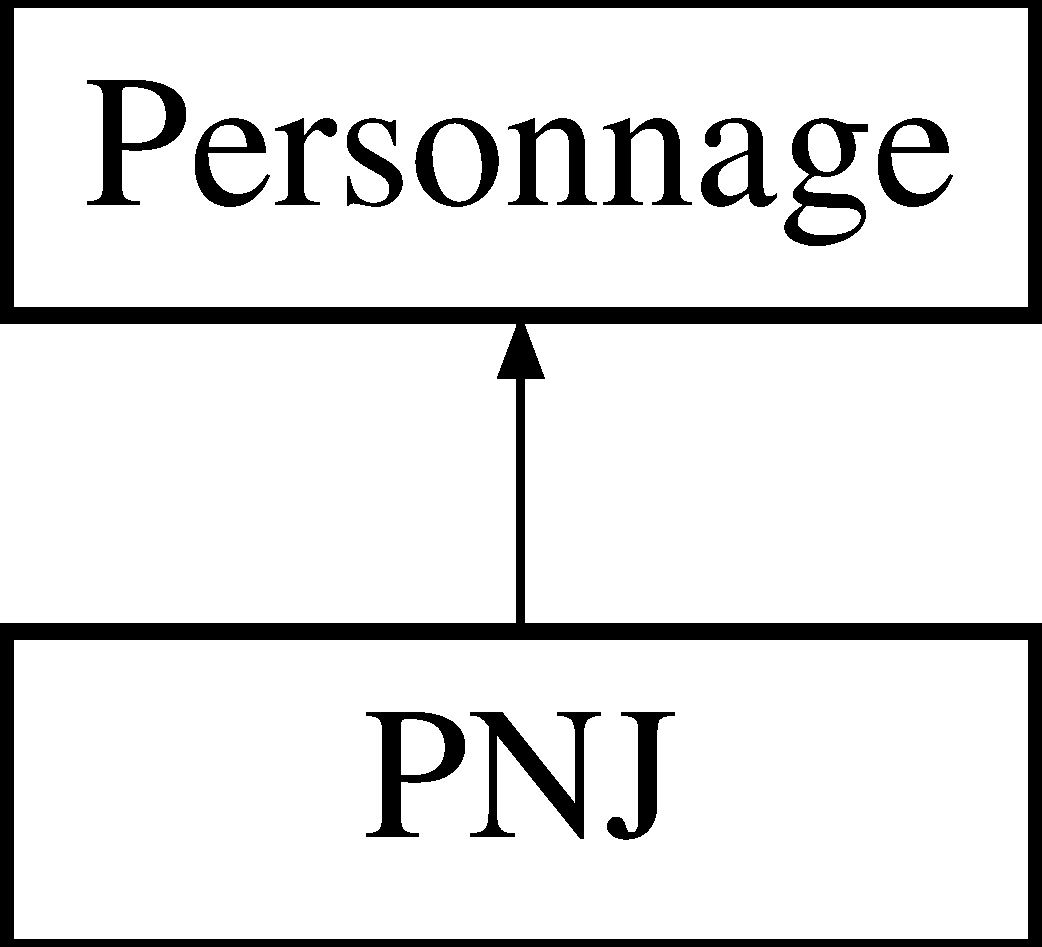
\includegraphics[height=2.000000cm]{class_p_n_j}
\end{center}
\end{figure}
\subsection*{Public Member Functions}
\begin{DoxyCompactItemize}
\item 
\hyperlink{class_p_n_j_af47e047679a553304cd94c4f052afc9d}{P\-N\-J} ()
\begin{DoxyCompactList}\small\item\em Constructeur par défaut. \end{DoxyCompactList}\item 
\hyperlink{class_p_n_j_a9d69e66223cac489b73561e71e0949e4}{P\-N\-J} (int intelp, int forcep, int agep, string nomp, vector$<$ \hyperlink{class_mission}{Mission} $\ast$ $>$ miss, string dpd)
\begin{DoxyCompactList}\small\item\em Constructeur de la classe \hyperlink{class_p_n_j}{P\-N\-J}. \end{DoxyCompactList}\item 
void \hyperlink{class_p_n_j_a519fb3ba5b692d2088c7c3a66421f72b}{set\-Missions\-P} (vector$<$ \hyperlink{class_mission}{Mission} $\ast$ $>$ new\-\_\-var)
\begin{DoxyCompactList}\small\item\em stock la valeur de la variable new\-\_\-var dans la variable Missions\-P. \end{DoxyCompactList}\item 
vector$<$ \hyperlink{class_mission}{Mission} $\ast$ $>$ \hyperlink{class_p_n_j_ab947fafa6afecf6640e1279ff05b7941}{get\-Missions\-P} ()
\begin{DoxyCompactList}\small\item\em Accède à la variable Mission\-P. \end{DoxyCompactList}\item 
string \hyperlink{class_p_n_j_ac2495e0c6580568cd6299389df128b20}{get\-Dialogue\-Par\-Defaut} ()
\begin{DoxyCompactList}\small\item\em Accède à la variable dialogue\-Par\-Defaut. \end{DoxyCompactList}\item 
void \hyperlink{class_p_n_j_ae938be01cfe4befe3a86c512cb2f87e1}{set\-Dialogue\-Par\-Defaut} (string dpd)
\begin{DoxyCompactList}\small\item\em stock la valeur de la variable dpd dans la variable Dialogue\-Par\-Defaut. \end{DoxyCompactList}\item 
string \hyperlink{class_p_n_j_a11332cced0b00f4dfb9221b2d897aba5}{get\-Nom\-P\-N\-J} ()
\begin{DoxyCompactList}\small\item\em Accède à la variable Nom\-P\-N\-J. \end{DoxyCompactList}\item 
void \hyperlink{class_p_n_j_a05bc22ba955f35343d89ef3d040d5fa4}{set\-Nom\-P\-N\-J} (string nomp)
\begin{DoxyCompactList}\small\item\em stock la valeur de la variable nomp dans la variable Nom\-P\-N\-J. \end{DoxyCompactList}\end{DoxyCompactItemize}
\subsection*{Additional Inherited Members}


\subsection{Detailed Description}
Classe représentant les \hyperlink{class_p_n_j}{P\-N\-J} (personnes non joueurs). 

\subsection{Constructor \& Destructor Documentation}
\hypertarget{class_p_n_j_af47e047679a553304cd94c4f052afc9d}{\index{P\-N\-J@{P\-N\-J}!P\-N\-J@{P\-N\-J}}
\index{P\-N\-J@{P\-N\-J}!PNJ@{P\-N\-J}}
\subsubsection[{P\-N\-J}]{\setlength{\rightskip}{0pt plus 5cm}P\-N\-J\-::\-P\-N\-J (
\begin{DoxyParamCaption}
{}
\end{DoxyParamCaption}
)}}\label{class_p_n_j_af47e047679a553304cd94c4f052afc9d}


Constructeur par défaut. 


\begin{DoxyCode}
9 \{\}
\end{DoxyCode}
\hypertarget{class_p_n_j_a9d69e66223cac489b73561e71e0949e4}{\index{P\-N\-J@{P\-N\-J}!P\-N\-J@{P\-N\-J}}
\index{P\-N\-J@{P\-N\-J}!PNJ@{P\-N\-J}}
\subsubsection[{P\-N\-J}]{\setlength{\rightskip}{0pt plus 5cm}P\-N\-J\-::\-P\-N\-J (
\begin{DoxyParamCaption}
\item[{int}]{intelp, }
\item[{int}]{forcep, }
\item[{int}]{agep, }
\item[{string}]{nomp, }
\item[{vector$<$ {\bf Mission} $\ast$ $>$}]{miss, }
\item[{string}]{dpd}
\end{DoxyParamCaption}
)}}\label{class_p_n_j_a9d69e66223cac489b73561e71e0949e4}


Constructeur de la classe \hyperlink{class_p_n_j}{P\-N\-J}. 


\begin{DoxyParams}{Parameters}
{\em intelp} & La valeur de l'intelligence du \hyperlink{class_p_n_j}{P\-N\-J}. \\
\hline
{\em forcep} & La valeur de la force du \hyperlink{class_p_n_j}{P\-N\-J}. \\
\hline
{\em agep} & L'âge du \hyperlink{class_p_n_j}{P\-N\-J}. \\
\hline
{\em nomp} & Le nom du \hyperlink{class_p_n_j}{P\-N\-J}. \\
\hline
{\em miss} & Le vecteur des missions proposées par les \hyperlink{class_p_n_j}{P\-N\-J}. \\
\hline
{\em dpd} & Le dialogue par défaut du \hyperlink{class_p_n_j}{P\-N\-J} \\
\hline
\end{DoxyParams}

\begin{DoxyCode}
11                                                                                          :
      \hyperlink{class_personnage_abec36eb0310adc71f3375297fc590c65}{Personnage}(intelp,forcep,agep,nomp)\{
12 
13     missionsP = miss;
14     dialogueParDefaut= dpd;
15     \}
\end{DoxyCode}


\subsection{Member Function Documentation}
\hypertarget{class_p_n_j_ac2495e0c6580568cd6299389df128b20}{\index{P\-N\-J@{P\-N\-J}!get\-Dialogue\-Par\-Defaut@{get\-Dialogue\-Par\-Defaut}}
\index{get\-Dialogue\-Par\-Defaut@{get\-Dialogue\-Par\-Defaut}!PNJ@{P\-N\-J}}
\subsubsection[{get\-Dialogue\-Par\-Defaut}]{\setlength{\rightskip}{0pt plus 5cm}string P\-N\-J\-::get\-Dialogue\-Par\-Defaut (
\begin{DoxyParamCaption}
{}
\end{DoxyParamCaption}
)}}\label{class_p_n_j_ac2495e0c6580568cd6299389df128b20}


Accède à la variable dialogue\-Par\-Defaut. 

\begin{DoxyReturn}{Returns}
Le dialogue par défaut du \hyperlink{class_p_n_j}{P\-N\-J}. 
\end{DoxyReturn}

\begin{DoxyCode}
32                                     \{
33     \textcolor{keywordflow}{return} dialogueParDefaut;
34   \}
\end{DoxyCode}
\hypertarget{class_p_n_j_ab947fafa6afecf6640e1279ff05b7941}{\index{P\-N\-J@{P\-N\-J}!get\-Missions\-P@{get\-Missions\-P}}
\index{get\-Missions\-P@{get\-Missions\-P}!PNJ@{P\-N\-J}}
\subsubsection[{get\-Missions\-P}]{\setlength{\rightskip}{0pt plus 5cm}vector$<$ {\bf Mission} $\ast$ $>$ P\-N\-J\-::get\-Missions\-P (
\begin{DoxyParamCaption}
{}
\end{DoxyParamCaption}
)}}\label{class_p_n_j_ab947fafa6afecf6640e1279ff05b7941}


Accède à la variable Mission\-P. 

\begin{DoxyReturn}{Returns}
Un vecteur de missions. 
\end{DoxyReturn}

\begin{DoxyCode}
28                                         \{
29     \textcolor{keywordflow}{return} missionsP;
30   \}
\end{DoxyCode}
\hypertarget{class_p_n_j_a11332cced0b00f4dfb9221b2d897aba5}{\index{P\-N\-J@{P\-N\-J}!get\-Nom\-P\-N\-J@{get\-Nom\-P\-N\-J}}
\index{get\-Nom\-P\-N\-J@{get\-Nom\-P\-N\-J}!PNJ@{P\-N\-J}}
\subsubsection[{get\-Nom\-P\-N\-J}]{\setlength{\rightskip}{0pt plus 5cm}string P\-N\-J\-::get\-Nom\-P\-N\-J (
\begin{DoxyParamCaption}
{}
\end{DoxyParamCaption}
)}}\label{class_p_n_j_a11332cced0b00f4dfb9221b2d897aba5}


Accède à la variable Nom\-P\-N\-J. 

\begin{DoxyReturn}{Returns}
Le nom du \hyperlink{class_p_n_j}{P\-N\-J}. 
\end{DoxyReturn}

\begin{DoxyCode}
20                        \{
21     \textcolor{keywordflow}{return} \hyperlink{class_personnage_acb7331b96dfc9f2aec78c60799030302}{nom};
22 \}
\end{DoxyCode}
\hypertarget{class_p_n_j_ae938be01cfe4befe3a86c512cb2f87e1}{\index{P\-N\-J@{P\-N\-J}!set\-Dialogue\-Par\-Defaut@{set\-Dialogue\-Par\-Defaut}}
\index{set\-Dialogue\-Par\-Defaut@{set\-Dialogue\-Par\-Defaut}!PNJ@{P\-N\-J}}
\subsubsection[{set\-Dialogue\-Par\-Defaut}]{\setlength{\rightskip}{0pt plus 5cm}void P\-N\-J\-::set\-Dialogue\-Par\-Defaut (
\begin{DoxyParamCaption}
\item[{string}]{dpd}
\end{DoxyParamCaption}
)}}\label{class_p_n_j_ae938be01cfe4befe3a86c512cb2f87e1}


stock la valeur de la variable dpd dans la variable Dialogue\-Par\-Defaut. 


\begin{DoxyCode}
36                                            \{
37     dialogueParDefaut = dpd;
38   \}
\end{DoxyCode}
\hypertarget{class_p_n_j_a519fb3ba5b692d2088c7c3a66421f72b}{\index{P\-N\-J@{P\-N\-J}!set\-Missions\-P@{set\-Missions\-P}}
\index{set\-Missions\-P@{set\-Missions\-P}!PNJ@{P\-N\-J}}
\subsubsection[{set\-Missions\-P}]{\setlength{\rightskip}{0pt plus 5cm}void P\-N\-J\-::set\-Missions\-P (
\begin{DoxyParamCaption}
\item[{vector$<$ {\bf Mission} $\ast$ $>$}]{new\-\_\-var}
\end{DoxyParamCaption}
)}}\label{class_p_n_j_a519fb3ba5b692d2088c7c3a66421f72b}


stock la valeur de la variable new\-\_\-var dans la variable Missions\-P. 


\begin{DoxyCode}
24                                                     \{
25       missionsP = new\_var;
26   \}
\end{DoxyCode}
\hypertarget{class_p_n_j_a05bc22ba955f35343d89ef3d040d5fa4}{\index{P\-N\-J@{P\-N\-J}!set\-Nom\-P\-N\-J@{set\-Nom\-P\-N\-J}}
\index{set\-Nom\-P\-N\-J@{set\-Nom\-P\-N\-J}!PNJ@{P\-N\-J}}
\subsubsection[{set\-Nom\-P\-N\-J}]{\setlength{\rightskip}{0pt plus 5cm}void P\-N\-J\-::set\-Nom\-P\-N\-J (
\begin{DoxyParamCaption}
\item[{string}]{nomp}
\end{DoxyParamCaption}
)}}\label{class_p_n_j_a05bc22ba955f35343d89ef3d040d5fa4}


stock la valeur de la variable nomp dans la variable Nom\-P\-N\-J. 


\begin{DoxyCode}
17                                 \{
18     \hyperlink{class_personnage_acb7331b96dfc9f2aec78c60799030302}{nom} = nomp;
19 \}
\end{DoxyCode}


The documentation for this class was generated from the following files\-:\begin{DoxyCompactItemize}
\item 
/nfs/usersgm/\-G\-M26/neljibbawe/\-Bureau/\-Projet\-C\-P\-P\-A\-Rendre/\-C\-P\-P R\-P\-G/\-R\-P\-G/\hyperlink{pnj_8hpp}{pnj.\-hpp}\item 
/nfs/usersgm/\-G\-M26/neljibbawe/\-Bureau/\-Projet\-C\-P\-P\-A\-Rendre/\-C\-P\-P R\-P\-G/\-R\-P\-G/\hyperlink{pnj_8cpp}{pnj.\-cpp}\end{DoxyCompactItemize}

\hypertarget{struct_q_c_m}{\section{Q\-C\-M Struct Reference}
\label{struct_q_c_m}\index{Q\-C\-M@{Q\-C\-M}}
}


{\ttfamily \#include $<$missionmaths.\-hpp$>$}

\subsection*{Public Attributes}
\begin{DoxyCompactItemize}
\item 
string \hyperlink{struct_q_c_m_a6d24b233b44048c23595712c0e03fb47}{exo}
\item 
int \hyperlink{struct_q_c_m_ad90e9b83f64b15f51e3f920922670fa4}{answer}
\end{DoxyCompactItemize}


\subsection{Member Data Documentation}
\hypertarget{struct_q_c_m_ad90e9b83f64b15f51e3f920922670fa4}{\index{Q\-C\-M@{Q\-C\-M}!answer@{answer}}
\index{answer@{answer}!QCM@{Q\-C\-M}}
\subsubsection[{answer}]{\setlength{\rightskip}{0pt plus 5cm}int Q\-C\-M\-::answer}}\label{struct_q_c_m_ad90e9b83f64b15f51e3f920922670fa4}
\hypertarget{struct_q_c_m_a6d24b233b44048c23595712c0e03fb47}{\index{Q\-C\-M@{Q\-C\-M}!exo@{exo}}
\index{exo@{exo}!QCM@{Q\-C\-M}}
\subsubsection[{exo}]{\setlength{\rightskip}{0pt plus 5cm}string Q\-C\-M\-::exo}}\label{struct_q_c_m_a6d24b233b44048c23595712c0e03fb47}


The documentation for this struct was generated from the following file\-:\begin{DoxyCompactItemize}
\item 
/nfs/usersgm/\-G\-M26/neljibbawe/\-Bureau/\-Projet\-C\-P\-P\-A\-Rendre/\-C\-P\-P R\-P\-G/\-R\-P\-G/\hyperlink{missionmaths_8hpp}{missionmaths.\-hpp}\end{DoxyCompactItemize}

\hypertarget{class_superette}{\section{Superette Class Reference}
\label{class_superette}\index{Superette@{Superette}}
}


Classe représentant la superette.  




{\ttfamily \#include $<$superette.\-hpp$>$}

Inheritance diagram for Superette\-:\begin{figure}[H]
\begin{center}
\leavevmode
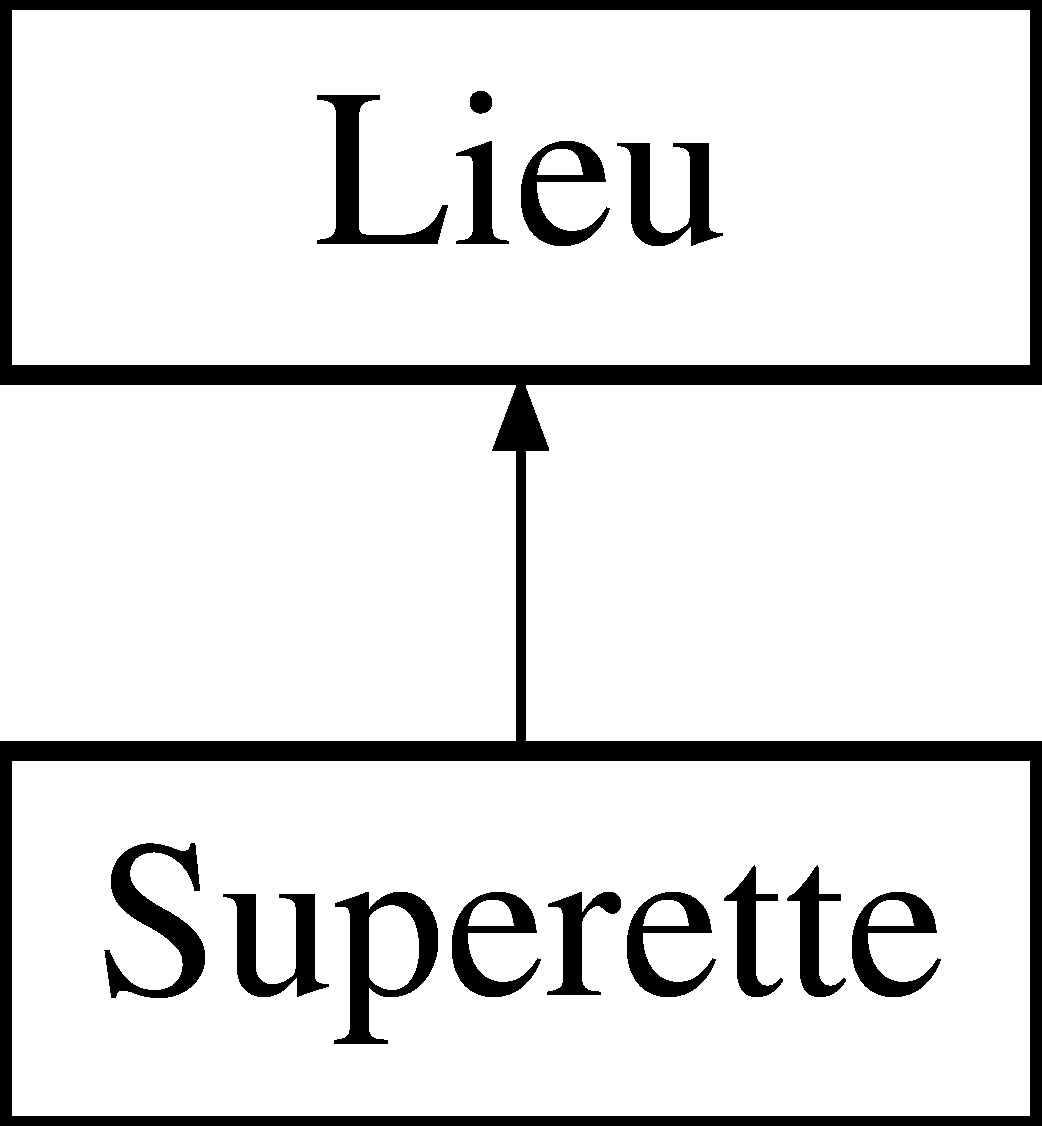
\includegraphics[height=2.000000cm]{class_superette}
\end{center}
\end{figure}
\subsection*{Public Member Functions}
\begin{DoxyCompactItemize}
\item 
\hyperlink{class_superette_a83beb054a37acf78f325a11e679d06c6}{Superette} ()
\begin{DoxyCompactList}\small\item\em Constructeur par défaut. \end{DoxyCompactList}\item 
\hyperlink{class_superette_af6ecf322ce825777c01851e8b64b9f1c}{Superette} (vector$<$ \hyperlink{class_objet}{Objet} $>$ \hyperlink{class_lieu_a3a65fbb8ecba3f2e265905730ad2e631}{objets\-Dispo}, int \hyperlink{class_lieu_a90b76b521f92a43626ccd29ed5a29f89}{cash\-Cache}, vector$<$ \hyperlink{class_p_n_j}{P\-N\-J} $>$ \hyperlink{class_lieu_a8c1e20b105f7972f22d8f16651de4ebd}{liste\-P\-N\-J}, string \hyperlink{class_lieu_a1e48889fe5c581f043b8bd77ca497fc7}{nom\-Lieu}, vector$<$ string $>$ action\-Vec, map$<$ string, \hyperlink{class_objet}{Objet} $>$ objets\-A\-Vendre)
\begin{DoxyCompactList}\small\item\em Constructeur de la classe superette. \end{DoxyCompactList}\item 
void \hyperlink{class_superette_a6c9124730932bbf721149f5167c0611d}{executer\-Action} (\hyperlink{class_jeu}{Jeu} jeu, \hyperlink{class_heros}{Heros} $\ast$heros, \hyperlink{class_ville}{Ville} $\ast$ville)
\begin{DoxyCompactList}\small\item\em Exécute une action parmi les actions possibles. \end{DoxyCompactList}\item 
void \hyperlink{class_superette_a03c5890e470b71e24e59e2b018286a18}{acheter\-Un\-Objet} (\hyperlink{class_heros}{Heros} $\ast$heros, \hyperlink{class_objet}{Objet} objet)
\begin{DoxyCompactList}\small\item\em Achète un objet parmi les objets disponibles dans la superette. \end{DoxyCompactList}\item 
void \hyperlink{class_superette_a4d3c1ec385b042f8cd59f7e592a134f2}{vendre\-Un\-Objet} (\hyperlink{class_heros}{Heros} $\ast$heros, \hyperlink{class_objet}{Objet} objet)
\begin{DoxyCompactList}\small\item\em Vend un objet parmi les objets disponibles dans le sac. \end{DoxyCompactList}\item 
const map$<$ string, \hyperlink{class_objet}{Objet} $>$ \& \hyperlink{class_superette_a38f21ad92a08b036ee3b50e3762c02fd}{get\-Objets\-A\-Vendre} () const 
\begin{DoxyCompactList}\small\item\em Accède à la variable objets\-A\-Vendre. \end{DoxyCompactList}\item 
void \hyperlink{class_superette_af203c4433fcb6831175aed1d18e7f05b}{set\-Objets\-A\-Vendre} (const map$<$ string, \hyperlink{class_objet}{Objet} $>$ \&objets\-A\-Vendre)
\begin{DoxyCompactList}\small\item\em stock la valeur de la variable \& objets\-A\-Vendre dans la variable objets\-A\-Vendre. \end{DoxyCompactList}\end{DoxyCompactItemize}
\subsection*{Additional Inherited Members}


\subsection{Detailed Description}
Classe représentant la superette. 

\subsection{Constructor \& Destructor Documentation}
\hypertarget{class_superette_a83beb054a37acf78f325a11e679d06c6}{\index{Superette@{Superette}!Superette@{Superette}}
\index{Superette@{Superette}!Superette@{Superette}}
\subsubsection[{Superette}]{\setlength{\rightskip}{0pt plus 5cm}Superette\-::\-Superette (
\begin{DoxyParamCaption}
{}
\end{DoxyParamCaption}
)}}\label{class_superette_a83beb054a37acf78f325a11e679d06c6}


Constructeur par défaut. 


\begin{DoxyCode}
19 \{\}
\end{DoxyCode}
\hypertarget{class_superette_af6ecf322ce825777c01851e8b64b9f1c}{\index{Superette@{Superette}!Superette@{Superette}}
\index{Superette@{Superette}!Superette@{Superette}}
\subsubsection[{Superette}]{\setlength{\rightskip}{0pt plus 5cm}Superette\-::\-Superette (
\begin{DoxyParamCaption}
\item[{vector$<$ {\bf Objet} $>$}]{objets\-Dispo, }
\item[{int}]{cash\-Cache, }
\item[{vector$<$ {\bf P\-N\-J} $>$}]{liste\-P\-N\-J, }
\item[{string}]{nom\-Lieu, }
\item[{vector$<$ string $>$}]{action\-Vec, }
\item[{map$<$ string, {\bf Objet} $>$}]{objets\-A\-Vendre}
\end{DoxyParamCaption}
)}}\label{class_superette_af6ecf322ce825777c01851e8b64b9f1c}


Constructeur de la classe superette. 


\begin{DoxyParams}{Parameters}
{\em objets\-Dispo} & Le vecteur des objets disponibles dans la superette. \\
\hline
{\em cashcache} & La valeur du cash caché dans la superette. \\
\hline
{\em liste\-P\-N\-J} & Le vecteur des \hyperlink{class_p_n_j}{P\-N\-J} présents dans la superette. \\
\hline
{\em nom\-Lieu} & Le nom de la superette. \\
\hline
{\em action\-Vec} & Le vecteur des actions possibles dans la superette. \\
\hline
{\em objets\-A\-Vendre} & Un map des objets à vendre dans la superette. \\
\hline
\end{DoxyParams}

\begin{DoxyCode}
20                                                                                                            
                                                           : \hyperlink{class_lieu_a0b3086d598fc1bfc0b4c09ae96304b3a}{Lieu} (\hyperlink{class_lieu_a3a65fbb8ecba3f2e265905730ad2e631}{objetsDispo}, 
      \hyperlink{class_lieu_a90b76b521f92a43626ccd29ed5a29f89}{cashCache}, \hyperlink{class_lieu_a8c1e20b105f7972f22d8f16651de4ebd}{listePNJ}, \textcolor{stringliteral}{"Superette"}, actionVec)\{
21     this->objetsAVendre = objetsAVendre;\}
\end{DoxyCode}


\subsection{Member Function Documentation}
\hypertarget{class_superette_a03c5890e470b71e24e59e2b018286a18}{\index{Superette@{Superette}!acheter\-Un\-Objet@{acheter\-Un\-Objet}}
\index{acheter\-Un\-Objet@{acheter\-Un\-Objet}!Superette@{Superette}}
\subsubsection[{acheter\-Un\-Objet}]{\setlength{\rightskip}{0pt plus 5cm}void Superette\-::acheter\-Un\-Objet (
\begin{DoxyParamCaption}
\item[{{\bf Heros} $\ast$}]{heros, }
\item[{{\bf Objet}}]{objet}
\end{DoxyParamCaption}
)}}\label{class_superette_a03c5890e470b71e24e59e2b018286a18}


Achète un objet parmi les objets disponibles dans la superette. 


\begin{DoxyParams}{Parameters}
{\em objet} & Un paramètre de la classe \hyperlink{class_objet}{Objet}. \\
\hline
{\em heros} & un paramètre de la classe \hyperlink{class_heros}{Heros}. \\
\hline
\end{DoxyParams}

\begin{DoxyCode}
165                                                             \{
166 
167         \textcolor{keywordflow}{if} ( heros->\hyperlink{class_heros_a77bdee21cb8c8356448bb6669941441c}{getCash}() >= objet.\hyperlink{class_objet_a9b36c37091e821bc8f00d6bfd3665a66}{getPrix}() ) \{
168 \textcolor{comment}{//          cout<<"jsikskqs "<<heros->getCash()<<endl;}
169 \textcolor{comment}{//          cout<<"jsikskqs "<<objet.getPrix()<<endl;}
170             heros->\hyperlink{class_heros_ae87dba7afa03e7fdacfc3a7e82d3a6a3}{setCash} ( heros->\hyperlink{class_heros_a77bdee21cb8c8356448bb6669941441c}{getCash}() - objet.\hyperlink{class_objet_a9b36c37091e821bc8f00d6bfd3665a66}{getPrix}() ) ;
171             map<string, Objet*> sacH=heros->\hyperlink{class_heros_a62d8b172e82dbb0a1d2c23da21bdb069}{getSac}();
172             sacH[objet.\hyperlink{class_objet_a843e99ecd1e150589f8db23f43dd27b0}{getNomObjet}()]->setQuantiteObjet( heros->
      \hyperlink{class_heros_a62d8b172e82dbb0a1d2c23da21bdb069}{getSac}()[objet.\hyperlink{class_objet_a843e99ecd1e150589f8db23f43dd27b0}{getNomObjet}()]->getQuantiteObjet()+1 ) ;
173             heros->\hyperlink{class_heros_a7d6d86388fe81deca1c5688ed07b2167}{setSac}(sacH);
174         \}
175     \}
\end{DoxyCode}
\hypertarget{class_superette_a6c9124730932bbf721149f5167c0611d}{\index{Superette@{Superette}!executer\-Action@{executer\-Action}}
\index{executer\-Action@{executer\-Action}!Superette@{Superette}}
\subsubsection[{executer\-Action}]{\setlength{\rightskip}{0pt plus 5cm}void Superette\-::executer\-Action (
\begin{DoxyParamCaption}
\item[{{\bf Jeu}}]{jeu, }
\item[{{\bf Heros} $\ast$}]{heros, }
\item[{{\bf Ville} $\ast$}]{ville}
\end{DoxyParamCaption}
)\hspace{0.3cm}{\ttfamily [virtual]}}}\label{class_superette_a6c9124730932bbf721149f5167c0611d}


Exécute une action parmi les actions possibles. 


\begin{DoxyParams}{Parameters}
{\em jeu} & Un paramètre de la classe \hyperlink{class_jeu}{Jeu}. \\
\hline
{\em heros} & un paramètre de la classe \hyperlink{class_heros}{Heros}. \\
\hline
\end{DoxyParams}


Reimplemented from \hyperlink{class_lieu_ad5d4e14283df04f0174f090f1614225c}{Lieu}.


\begin{DoxyCode}
42                                                                       \{
43 
44         \textcolor{keywordtype}{int} i=0, entree = -1 ;
45     \textcolor{keywordflow}{while} (entree!=i+5) \{
46 
47         jeu.\hyperlink{class_jeu_aa09fb40439f16b9665a0d76679f78e4e}{afficherTexte}( \textcolor{stringliteral}{"Vous êtes dans le lieu suivant : "} + 
      \hyperlink{class_lieu_a1e48889fe5c581f043b8bd77ca497fc7}{nomLieu} + \textcolor{stringliteral}{". Que voulez-vous faire ? (entrée attendue : un numéro)"} );
48 
49 
50         \textcolor{keywordflow}{for} (i=0 ; i < \hyperlink{class_lieu_a8c1e20b105f7972f22d8f16651de4ebd}{listePNJ}.size(); i++) \{
51 
52         jeu.\hyperlink{class_jeu_aa09fb40439f16b9665a0d76679f78e4e}{afficherTexte}(\hyperlink{superette_8cpp_a0d2f37137ee1fd6ff4a0ef803849dd63}{SSTR}(i) + \textcolor{stringliteral}{". Parler à la personne suivante :"} + 
      \hyperlink{class_lieu_a8c1e20b105f7972f22d8f16651de4ebd}{listePNJ}.at(i).getNom() );
53         \}
54 
55         jeu.\hyperlink{class_jeu_aa09fb40439f16b9665a0d76679f78e4e}{afficherTexte}(\hyperlink{superette_8cpp_a0d2f37137ee1fd6ff4a0ef803849dd63}{SSTR}(i) + \textcolor{stringliteral}{". "} + \textcolor{stringliteral}{"Acheter"} );
56 
57         jeu.\hyperlink{class_jeu_aa09fb40439f16b9665a0d76679f78e4e}{afficherTexte}(\hyperlink{superette_8cpp_a0d2f37137ee1fd6ff4a0ef803849dd63}{SSTR}(i+1) + \textcolor{stringliteral}{". "} + \textcolor{stringliteral}{"Vendre"} );
58 
59         jeu.\hyperlink{class_jeu_aa09fb40439f16b9665a0d76679f78e4e}{afficherTexte}(\hyperlink{superette_8cpp_a0d2f37137ee1fd6ff4a0ef803849dd63}{SSTR}(i+2) + \textcolor{stringliteral}{". "} + \textcolor{stringliteral}{"Fouiller"} );
60 
61         jeu.\hyperlink{class_jeu_aa09fb40439f16b9665a0d76679f78e4e}{afficherTexte}(\hyperlink{superette_8cpp_a0d2f37137ee1fd6ff4a0ef803849dd63}{SSTR}(i+3) + \textcolor{stringliteral}{". "} + \textcolor{stringliteral}{"Afficher Sac"} );
62 
63         jeu.\hyperlink{class_jeu_aa09fb40439f16b9665a0d76679f78e4e}{afficherTexte}(\hyperlink{superette_8cpp_a0d2f37137ee1fd6ff4a0ef803849dd63}{SSTR}(i+4) + \textcolor{stringliteral}{". "} + \textcolor{stringliteral}{"Afficher Stats du Héros"} );
64 
65         jeu.\hyperlink{class_jeu_aa09fb40439f16b9665a0d76679f78e4e}{afficherTexte}(\hyperlink{superette_8cpp_a0d2f37137ee1fd6ff4a0ef803849dd63}{SSTR}(i+5) + \textcolor{stringliteral}{". "} + \textcolor{stringliteral}{"Quitter"} );
66 
67 
68 
69         entree = jeu.\hyperlink{class_jeu_ac504a2a26ad7aa3c4281f8ab40cdc445}{demanderEntreeUtilisateur}(\textcolor{stringliteral}{"Faites votre choix :"});
70         \textcolor{keywordflow}{while} (entree < 0 or entree > i+5) \{
71             entree = jeu.\hyperlink{class_jeu_ac504a2a26ad7aa3c4281f8ab40cdc445}{demanderEntreeUtilisateur}(\textcolor{stringliteral}{"Faites un choix CORRECT :"});
72         \}
73 
74         \textcolor{keywordflow}{if} ( entree >= 0 and entree < i )
75             jeu.\hyperlink{class_jeu_aa09fb40439f16b9665a0d76679f78e4e}{afficherTexte}( heros->\hyperlink{class_heros_a4052af6e407ebdf4918e62340d374829}{ParleAPNJ}(&\hyperlink{class_lieu_a8c1e20b105f7972f22d8f16651de4ebd}{listePNJ}.at(entree), jeu) ) 
      ;
76 
77         \textcolor{keywordflow}{else} \textcolor{keywordflow}{if} ( entree == i )\{
78 
79             jeu.\hyperlink{class_jeu_aa09fb40439f16b9665a0d76679f78e4e}{afficherTexte}( \textcolor{stringliteral}{"Voici les objets à acheter :"} );
80             map<std::string,Objet>::iterator iit = objetsAVendre.begin();
81             map<std::string,Objet>::iterator iitt = objetsAVendre.end();
82             \textcolor{keywordflow}{while} ( iit != iitt )
83             \{
84                 jeu.\hyperlink{class_jeu_aa09fb40439f16b9665a0d76679f78e4e}{afficherTexte}( (*iit).first + \textcolor{stringliteral}{" - Prix: "} +  
      \hyperlink{superette_8cpp_a0d2f37137ee1fd6ff4a0ef803849dd63}{SSTR}((*iit).second.getPrix())   );
85                 iit++;
86             \}
87 
88             \textcolor{keywordtype}{string} choixObjet ;
89 
90             \textcolor{keywordflow}{do} \{
91             choixObjet = jeu.\hyperlink{class_jeu_a4b70e906117c6a21b989ad3ab672c83c}{demanderStringUtilisateur}(\textcolor{stringliteral}{"Quel objet voulez-vous
       acheter ? Ecrivez un objet valide, ou q pour retourner au menu"});
92             \} \textcolor{keywordflow}{while} ( choixObjet!=\textcolor{stringliteral}{"q"} && objetsAVendre.find(choixObjet) == objetsAVendre.end() );
93 
94             \textcolor{keywordflow}{if} (choixObjet!=\textcolor{stringliteral}{"q"}) \{
95                 \hyperlink{class_superette_a03c5890e470b71e24e59e2b018286a18}{acheterUnObjet}(heros, objetsAVendre[choixObjet]);
96                 jeu.\hyperlink{class_jeu_aa09fb40439f16b9665a0d76679f78e4e}{afficherTexte}(\textcolor{stringliteral}{"Vous avez acheté: "} + choixObjet + \textcolor{stringliteral}{". Nouvelle quantité de
       l'objet: "} + \hyperlink{superette_8cpp_a0d2f37137ee1fd6ff4a0ef803849dd63}{SSTR}(heros->\hyperlink{class_heros_a62d8b172e82dbb0a1d2c23da21bdb069}{getSac}()[choixObjet]->getQuantiteObjet()) + \textcolor{stringliteral}{". Nouveau cash: "} + 
      \hyperlink{superette_8cpp_a0d2f37137ee1fd6ff4a0ef803849dd63}{SSTR}(heros->\hyperlink{class_heros_a77bdee21cb8c8356448bb6669941441c}{getCash}()));
97             \}
98 
99         \}
100 
101         \textcolor{keywordflow}{else} \textcolor{keywordflow}{if} ( entree == i+1 )\{
102 
103             jeu.\hyperlink{class_jeu_aa09fb40439f16b9665a0d76679f78e4e}{afficherTexte}( \textcolor{stringliteral}{"Voici vos objets que vous pouvez vendre :"} );
104             map<string, Objet*> sacH = heros->\hyperlink{class_heros_a62d8b172e82dbb0a1d2c23da21bdb069}{getSac}();
105             map<string, Objet*>::iterator it = sacH.begin();
106             map<string, Objet*>::iterator iitt = sacH.end();
107             \textcolor{keywordflow}{while} ( it != iitt )
108             \{
109                 \textcolor{keywordflow}{if} ((*it).second->getQuantiteObjet() > 0)
110                     jeu.\hyperlink{class_jeu_aa09fb40439f16b9665a0d76679f78e4e}{afficherTexte}( (*it).first + \textcolor{stringliteral}{" - Prix: "} +  
      \hyperlink{superette_8cpp_a0d2f37137ee1fd6ff4a0ef803849dd63}{SSTR}((*it).second->getPrix())   + \textcolor{stringliteral}{" - Qté restante: "} +  \hyperlink{superette_8cpp_a0d2f37137ee1fd6ff4a0ef803849dd63}{SSTR}((*it).second->getQuantiteObjet()) );
111                 it++;
112             \}
113 
114             \textcolor{keywordtype}{string} choixObjet ;
115 
116 \textcolor{comment}{//          choixObjet = jeu.demanderStringUtilisateur("Quel objet voulez-vous vendre ? Ecrivez un objet
       valide, ou quitter pour retourner au menu");}
117 \textcolor{comment}{//                      vendreUnObjet(heros, heros->getSac()[choixObjet]);}
118 
119             \textcolor{keywordflow}{do} \{
120                 choixObjet = jeu.\hyperlink{class_jeu_a4b70e906117c6a21b989ad3ab672c83c}{demanderStringUtilisateur}(\textcolor{stringliteral}{"Quel objet voulez-vous
       vendre ? Ecrivez un objet valide, ou q pour retourner au menu"});
121             \} \textcolor{keywordflow}{while} ( choixObjet!=\textcolor{stringliteral}{"q"} && sacH.find(choixObjet) == sacH.end() );
122 
123             \textcolor{keywordflow}{if} (choixObjet!=\textcolor{stringliteral}{"q"}) \{
124                 \textcolor{keywordflow}{if} ( objetsAVendre[choixObjet].getQuantiteObjet() > 0) \{
125                     \hyperlink{class_superette_a4d3c1ec385b042f8cd59f7e592a134f2}{vendreUnObjet}(heros, *sacH[choixObjet]);
126                     jeu.\hyperlink{class_jeu_aa09fb40439f16b9665a0d76679f78e4e}{afficherTexte}(\textcolor{stringliteral}{"Vous avez vendu: "} + choixObjet + \textcolor{stringliteral}{". Nouvelle quantité
       de l'objet: "} + \hyperlink{superette_8cpp_a0d2f37137ee1fd6ff4a0ef803849dd63}{SSTR}(sacH[choixObjet]->getQuantiteObjet()) + \textcolor{stringliteral}{". Nouveau cash: "} + 
      \hyperlink{superette_8cpp_a0d2f37137ee1fd6ff4a0ef803849dd63}{SSTR}(heros->\hyperlink{class_heros_a77bdee21cb8c8356448bb6669941441c}{getCash}()));
127 
128                 \}
129                 \textcolor{keywordflow}{else} jeu.\hyperlink{class_jeu_aa09fb40439f16b9665a0d76679f78e4e}{afficherTexte}(\textcolor{stringliteral}{"Vous n'avez pas cet objet"});
130 
131             \}
132 
133         \}
134 
135         \textcolor{keywordflow}{else} \textcolor{keywordflow}{if} ( entree == i+2 )\{
136 
137             \hyperlink{class_lieu_a90d7fd86c93e59830e20156ddb7aeb50}{fouiller}(jeu, heros);
138 
139         \}
140 
141         \textcolor{keywordflow}{else} \textcolor{keywordflow}{if} ( entree == i+3 )\{
142 
143             jeu.\hyperlink{class_jeu_a26c7a428a96b1f987150cb708fa7d903}{consommersac}(heros);
144 
145         \}
146 
147         \textcolor{keywordflow}{else} \textcolor{keywordflow}{if} ( entree == i+4 )\{
148 
149             jeu.\hyperlink{class_jeu_a7f9e3b8e6f3ad5d2c47ae29c54f2bdc4}{affichageStatsHero}(*heros);
150 
151         \}
152 
153         \textcolor{keywordflow}{else} \textcolor{keywordflow}{if} ( entree == i+5 )\{
154             jeu.\hyperlink{class_jeu_a52ce4fb6c415b45209db13a589c9d675}{timer}(4, \textcolor{stringliteral}{"retour à la ville"});
155             heros->\hyperlink{class_heros_a8decc0b04f6724de10d2e2a8d1c3395c}{setLieuActuel}(ville);
156 
157         \}
158 
159         \textcolor{keywordflow}{else} \{\}
160 
161     \}
162     \}
\end{DoxyCode}
\hypertarget{class_superette_a38f21ad92a08b036ee3b50e3762c02fd}{\index{Superette@{Superette}!get\-Objets\-A\-Vendre@{get\-Objets\-A\-Vendre}}
\index{get\-Objets\-A\-Vendre@{get\-Objets\-A\-Vendre}!Superette@{Superette}}
\subsubsection[{get\-Objets\-A\-Vendre}]{\setlength{\rightskip}{0pt plus 5cm}const map$<$ string, {\bf Objet} $>$ \& Superette\-::get\-Objets\-A\-Vendre (
\begin{DoxyParamCaption}
{}
\end{DoxyParamCaption}
) const}}\label{class_superette_a38f21ad92a08b036ee3b50e3762c02fd}


Accède à la variable objets\-A\-Vendre. 

\begin{DoxyReturn}{Returns}
Le map des objets à vendre. 
\end{DoxyReturn}

\begin{DoxyCode}
34                                                             \{
35         \textcolor{keywordflow}{return} objetsAVendre;
36     \}
\end{DoxyCode}
\hypertarget{class_superette_af203c4433fcb6831175aed1d18e7f05b}{\index{Superette@{Superette}!set\-Objets\-A\-Vendre@{set\-Objets\-A\-Vendre}}
\index{set\-Objets\-A\-Vendre@{set\-Objets\-A\-Vendre}!Superette@{Superette}}
\subsubsection[{set\-Objets\-A\-Vendre}]{\setlength{\rightskip}{0pt plus 5cm}void Superette\-::set\-Objets\-A\-Vendre (
\begin{DoxyParamCaption}
\item[{const map$<$ string, {\bf Objet} $>$ \&}]{objets\-A\-Vendre}
\end{DoxyParamCaption}
)}}\label{class_superette_af203c4433fcb6831175aed1d18e7f05b}


stock la valeur de la variable \& objets\-A\-Vendre dans la variable objets\-A\-Vendre. 


\begin{DoxyCode}
38                                                                             \{
39         this->objetsAVendre = objetsAVendre;
40     \}
\end{DoxyCode}
\hypertarget{class_superette_a4d3c1ec385b042f8cd59f7e592a134f2}{\index{Superette@{Superette}!vendre\-Un\-Objet@{vendre\-Un\-Objet}}
\index{vendre\-Un\-Objet@{vendre\-Un\-Objet}!Superette@{Superette}}
\subsubsection[{vendre\-Un\-Objet}]{\setlength{\rightskip}{0pt plus 5cm}void Superette\-::vendre\-Un\-Objet (
\begin{DoxyParamCaption}
\item[{{\bf Heros} $\ast$}]{heros, }
\item[{{\bf Objet}}]{objet}
\end{DoxyParamCaption}
)}}\label{class_superette_a4d3c1ec385b042f8cd59f7e592a134f2}


Vend un objet parmi les objets disponibles dans le sac. 


\begin{DoxyParams}{Parameters}
{\em objet} & Un paramètre de la classe \hyperlink{class_objet}{Objet}. \\
\hline
{\em heros} & un paramètre de la classe \hyperlink{class_heros}{Heros}. \\
\hline
\end{DoxyParams}

\begin{DoxyCode}
177                                                            \{
178         
179         \textcolor{keywordflow}{if} ( heros->\hyperlink{class_heros_a62d8b172e82dbb0a1d2c23da21bdb069}{getSac}()[objet.\hyperlink{class_objet_a843e99ecd1e150589f8db23f43dd27b0}{getNomObjet}()]->getQuantiteObjet() > 0 ) \{
180         
181             heros->\hyperlink{class_heros_ae87dba7afa03e7fdacfc3a7e82d3a6a3}{setCash} ( heros->\hyperlink{class_heros_a77bdee21cb8c8356448bb6669941441c}{getCash}() + objet.\hyperlink{class_objet_a9b36c37091e821bc8f00d6bfd3665a66}{getPrix}() ) ;
182             map<string, Objet*> sacH=heros->\hyperlink{class_heros_a62d8b172e82dbb0a1d2c23da21bdb069}{getSac}();
183             sacH[objet.\hyperlink{class_objet_a843e99ecd1e150589f8db23f43dd27b0}{getNomObjet}()]->setQuantiteObjet( heros->
      \hyperlink{class_heros_a62d8b172e82dbb0a1d2c23da21bdb069}{getSac}()[objet.\hyperlink{class_objet_a843e99ecd1e150589f8db23f43dd27b0}{getNomObjet}()]->getQuantiteObjet()-1 ) ;
184             heros->\hyperlink{class_heros_a7d6d86388fe81deca1c5688ed07b2167}{setSac}(sacH);
185 
186         \}
187     \}
\end{DoxyCode}


The documentation for this class was generated from the following files\-:\begin{DoxyCompactItemize}
\item 
/nfs/usersgm/\-G\-M26/neljibbawe/\-Bureau/\-Projet\-C\-P\-P\-A\-Rendre/\-C\-P\-P R\-P\-G/\-R\-P\-G/\hyperlink{superette_8hpp}{superette.\-hpp}\item 
/nfs/usersgm/\-G\-M26/neljibbawe/\-Bureau/\-Projet\-C\-P\-P\-A\-Rendre/\-C\-P\-P R\-P\-G/\-R\-P\-G/\hyperlink{superette_8cpp}{superette.\-cpp}\end{DoxyCompactItemize}

\hypertarget{class_ville}{\section{Ville Class Reference}
\label{class_ville}\index{Ville@{Ville}}
}


Classe représentant la ville.  




{\ttfamily \#include $<$ville.\-hpp$>$}

Inheritance diagram for Ville\-:\begin{figure}[H]
\begin{center}
\leavevmode
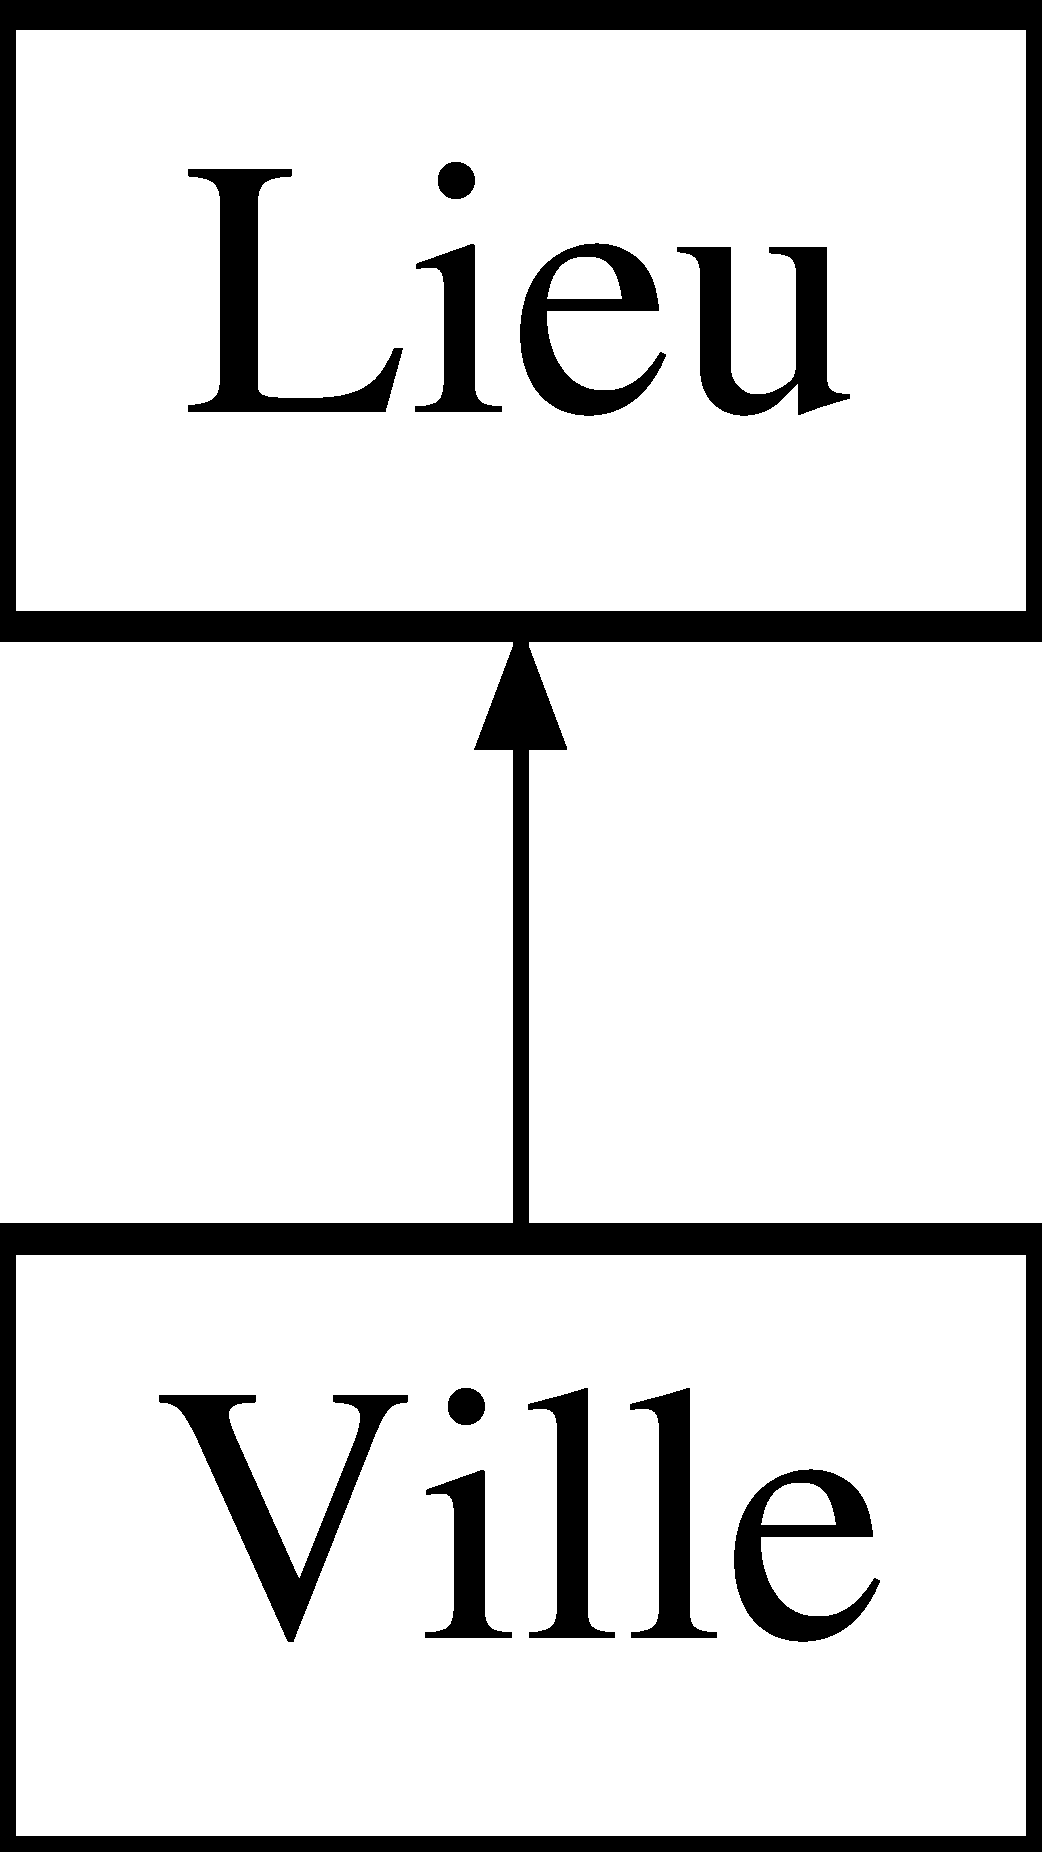
\includegraphics[height=2.000000cm]{class_ville}
\end{center}
\end{figure}
\subsection*{Public Member Functions}
\begin{DoxyCompactItemize}
\item 
\hyperlink{class_ville_a19a413ad16568980b527b5047399c585}{Ville} ()
\begin{DoxyCompactList}\small\item\em Constructeur par défaut. \end{DoxyCompactList}\item 
\hyperlink{class_ville_a0d8ae3c8e779b5918fe4c76095ffa73d}{Ville} (vector$<$ \hyperlink{class_objet}{Objet} $>$ \hyperlink{class_lieu_a3a65fbb8ecba3f2e265905730ad2e631}{objets\-Dispo}, int \hyperlink{class_lieu_a90b76b521f92a43626ccd29ed5a29f89}{cash\-Cache}, vector$<$ \hyperlink{class_p_n_j}{P\-N\-J} $>$ \hyperlink{class_lieu_a8c1e20b105f7972f22d8f16651de4ebd}{liste\-P\-N\-J}, string \hyperlink{class_lieu_a1e48889fe5c581f043b8bd77ca497fc7}{nom\-Lieu}, vector$<$ string $>$ action\-Vec, vector$<$ \hyperlink{class_lieu}{Lieu} $\ast$ $>$ lieu\-Vec)
\begin{DoxyCompactList}\small\item\em Constructeur de la classe ville. \end{DoxyCompactList}\item 
void \hyperlink{class_ville_a7bfe737f37ec9a99bc1e809047ca0e2e}{executer\-Action} (\hyperlink{class_jeu}{Jeu} jeu, \hyperlink{class_heros}{Heros} $\ast$heros, \hyperlink{class_ville}{Ville} $\ast$ville)
\begin{DoxyCompactList}\small\item\em Exécute une action parmi les actions possibles. \end{DoxyCompactList}\item 
void \hyperlink{class_ville_a533804907c678efb9a4e6f6dd0edac58}{initialiser\-Ville} ()
\begin{DoxyCompactList}\small\item\em Initialise la ville. \end{DoxyCompactList}\item 
const vector$<$ \hyperlink{class_lieu}{Lieu} $\ast$ $>$ \& \hyperlink{class_ville_a2a778c77b3c4d60b414807bc350e10ec}{get\-Lieu\-Vec} () const 
\begin{DoxyCompactList}\small\item\em Accède à la variable lieu\-Vec. \end{DoxyCompactList}\item 
void \hyperlink{class_ville_a64a43e83e7666ca2b157aea711b3bd2f}{set\-Lieu\-Vec} (const vector$<$ \hyperlink{class_lieu}{Lieu} $\ast$ $>$ \&lieu\-Vec)
\begin{DoxyCompactList}\small\item\em stock la valeur de la variable \& lieu\-Vec dans la variable lieu\-Vec. \end{DoxyCompactList}\end{DoxyCompactItemize}
\subsection*{Additional Inherited Members}


\subsection{Detailed Description}
Classe représentant la ville. 

\subsection{Constructor \& Destructor Documentation}
\hypertarget{class_ville_a19a413ad16568980b527b5047399c585}{\index{Ville@{Ville}!Ville@{Ville}}
\index{Ville@{Ville}!Ville@{Ville}}
\subsubsection[{Ville}]{\setlength{\rightskip}{0pt plus 5cm}Ville\-::\-Ville (
\begin{DoxyParamCaption}
{}
\end{DoxyParamCaption}
)}}\label{class_ville_a19a413ad16568980b527b5047399c585}


Constructeur par défaut. 


\begin{DoxyCode}
18 \{\}
\end{DoxyCode}
\hypertarget{class_ville_a0d8ae3c8e779b5918fe4c76095ffa73d}{\index{Ville@{Ville}!Ville@{Ville}}
\index{Ville@{Ville}!Ville@{Ville}}
\subsubsection[{Ville}]{\setlength{\rightskip}{0pt plus 5cm}Ville\-::\-Ville (
\begin{DoxyParamCaption}
\item[{vector$<$ {\bf Objet} $>$}]{objets\-Dispo, }
\item[{int}]{cash\-Cache, }
\item[{vector$<$ {\bf P\-N\-J} $>$}]{liste\-P\-N\-J, }
\item[{string}]{nom\-Lieu, }
\item[{vector$<$ string $>$}]{action\-Vec, }
\item[{vector$<$ {\bf Lieu} $\ast$ $>$}]{lieu\-Vec}
\end{DoxyParamCaption}
)}}\label{class_ville_a0d8ae3c8e779b5918fe4c76095ffa73d}


Constructeur de la classe ville. 


\begin{DoxyParams}{Parameters}
{\em lieu\-Vec} & Le vecteur des lieux possibles. \\
\hline
\end{DoxyParams}

\begin{DoxyCode}
20                                                                                                            
                                       : \hyperlink{class_lieu_a0b3086d598fc1bfc0b4c09ae96304b3a}{Lieu}(\hyperlink{class_lieu_a3a65fbb8ecba3f2e265905730ad2e631}{objetsDispo}, \hyperlink{class_lieu_a90b76b521f92a43626ccd29ed5a29f89}{cashCache}, 
      \hyperlink{class_lieu_a8c1e20b105f7972f22d8f16651de4ebd}{listePNJ}, \hyperlink{class_lieu_a1e48889fe5c581f043b8bd77ca497fc7}{nomLieu}, actionVec)\{
21     this->lieuVec = lieuVec;
22 \}
\end{DoxyCode}


\subsection{Member Function Documentation}
\hypertarget{class_ville_a7bfe737f37ec9a99bc1e809047ca0e2e}{\index{Ville@{Ville}!executer\-Action@{executer\-Action}}
\index{executer\-Action@{executer\-Action}!Ville@{Ville}}
\subsubsection[{executer\-Action}]{\setlength{\rightskip}{0pt plus 5cm}void Ville\-::executer\-Action (
\begin{DoxyParamCaption}
\item[{{\bf Jeu}}]{jeu, }
\item[{{\bf Heros} $\ast$}]{heros, }
\item[{{\bf Ville} $\ast$}]{ville}
\end{DoxyParamCaption}
)\hspace{0.3cm}{\ttfamily [virtual]}}}\label{class_ville_a7bfe737f37ec9a99bc1e809047ca0e2e}


Exécute une action parmi les actions possibles. 


\begin{DoxyParams}{Parameters}
{\em jeu} & Un paramètre de la classe \hyperlink{class_jeu}{Jeu}. \\
\hline
{\em heros} & un paramètre de la classe \hyperlink{class_heros}{Heros}. \\
\hline
\end{DoxyParams}


Reimplemented from \hyperlink{class_lieu_ad5d4e14283df04f0174f090f1614225c}{Lieu}.


\begin{DoxyCode}
33                                                               \{
34 
35         jeu.\hyperlink{class_jeu_aa09fb40439f16b9665a0d76679f78e4e}{afficherTexte}( \textcolor{stringliteral}{"\(\backslash\)nVous êtes dans le lieu suivant : "} + 
      \hyperlink{class_lieu_a1e48889fe5c581f043b8bd77ca497fc7}{nomLieu} + \textcolor{stringliteral}{". Que voulez-vous faire ?\(\backslash\)n"} );
36 
37         \textcolor{keywordtype}{int} i=0 ;
38         \textcolor{keywordflow}{for} (i=0 ; i < lieuVec.size(); i++) \{
39             jeu.\hyperlink{class_jeu_aa09fb40439f16b9665a0d76679f78e4e}{afficherTexte}( \hyperlink{ville_8cpp_a0d2f37137ee1fd6ff4a0ef803849dd63}{SSTR}(i) + \textcolor{stringliteral}{". Se rendre au lieu suivant :"} + this->lieuVec.
      at(i)->getNomLieu() );
40         \}
41         \textcolor{keywordtype}{int} entree = -1 ;
42         \textcolor{keywordflow}{while} (entree < 0 or entree > i-1) \{
43             entree = jeu.\hyperlink{class_jeu_ac504a2a26ad7aa3c4281f8ab40cdc445}{demanderEntreeUtilisateur}(\textcolor{stringliteral}{"Faites votre choix :"});
44         \}
45 
46         \textcolor{keywordflow}{if} ( entree >= 0 and entree < i ) \{
47             jeu.\hyperlink{class_jeu_a52ce4fb6c415b45209db13a589c9d675}{timer}(4, \textcolor{stringliteral}{"déplacement en cours..."});
48             heros->\hyperlink{class_heros_a8decc0b04f6724de10d2e2a8d1c3395c}{setLieuActuel}(lieuVec[entree]) ;
49         \}
50 
51         \textcolor{keywordflow}{else} \{\}
52 
53 
54 \}
\end{DoxyCode}
\hypertarget{class_ville_a2a778c77b3c4d60b414807bc350e10ec}{\index{Ville@{Ville}!get\-Lieu\-Vec@{get\-Lieu\-Vec}}
\index{get\-Lieu\-Vec@{get\-Lieu\-Vec}!Ville@{Ville}}
\subsubsection[{get\-Lieu\-Vec}]{\setlength{\rightskip}{0pt plus 5cm}const vector$<$ {\bf Lieu} $\ast$ $>$ \& Ville\-::get\-Lieu\-Vec (
\begin{DoxyParamCaption}
{}
\end{DoxyParamCaption}
) const}}\label{class_ville_a2a778c77b3c4d60b414807bc350e10ec}


Accède à la variable lieu\-Vec. 

\begin{DoxyReturn}{Returns}
le vecteur des lieux possibles. 
\end{DoxyReturn}

\begin{DoxyCode}
24                                              \{
25     \textcolor{keywordflow}{return} lieuVec;
26 \}
\end{DoxyCode}
\hypertarget{class_ville_a533804907c678efb9a4e6f6dd0edac58}{\index{Ville@{Ville}!initialiser\-Ville@{initialiser\-Ville}}
\index{initialiser\-Ville@{initialiser\-Ville}!Ville@{Ville}}
\subsubsection[{initialiser\-Ville}]{\setlength{\rightskip}{0pt plus 5cm}void Ville\-::initialiser\-Ville (
\begin{DoxyParamCaption}
{}
\end{DoxyParamCaption}
)}}\label{class_ville_a533804907c678efb9a4e6f6dd0edac58}


Initialise la ville. 


\begin{DoxyCode}
57                             \{
58     
59 \}
\end{DoxyCode}
\hypertarget{class_ville_a64a43e83e7666ca2b157aea711b3bd2f}{\index{Ville@{Ville}!set\-Lieu\-Vec@{set\-Lieu\-Vec}}
\index{set\-Lieu\-Vec@{set\-Lieu\-Vec}!Ville@{Ville}}
\subsubsection[{set\-Lieu\-Vec}]{\setlength{\rightskip}{0pt plus 5cm}void Ville\-::set\-Lieu\-Vec (
\begin{DoxyParamCaption}
\item[{const vector$<$ {\bf Lieu} $\ast$ $>$ \&}]{lieu\-Vec}
\end{DoxyParamCaption}
)}}\label{class_ville_a64a43e83e7666ca2b157aea711b3bd2f}


stock la valeur de la variable \& lieu\-Vec dans la variable lieu\-Vec. 


\begin{DoxyCode}
28                                                    \{
29     this->lieuVec = lieuVec;
30 \}
\end{DoxyCode}


The documentation for this class was generated from the following files\-:\begin{DoxyCompactItemize}
\item 
/nfs/usersgm/\-G\-M26/neljibbawe/\-Bureau/\-Projet\-C\-P\-P\-A\-Rendre/\-C\-P\-P R\-P\-G/\-R\-P\-G/\hyperlink{ville_8hpp}{ville.\-hpp}\item 
/nfs/usersgm/\-G\-M26/neljibbawe/\-Bureau/\-Projet\-C\-P\-P\-A\-Rendre/\-C\-P\-P R\-P\-G/\-R\-P\-G/\hyperlink{ville_8cpp}{ville.\-cpp}\end{DoxyCompactItemize}

\chapter{File Documentation}
\hypertarget{banque_8cpp}{\section{/nfs/usersgm/\-G\-M26/neljibbawe/\-Bureau/\-Projet\-C\-P\-P\-A\-Rendre/\-C\-P\-P R\-P\-G/\-R\-P\-G/banque.cpp File Reference}
\label{banque_8cpp}\index{/nfs/usersgm/\-G\-M26/neljibbawe/\-Bureau/\-Projet\-C\-P\-P\-A\-Rendre/\-C\-P\-P R\-P\-G/\-R\-P\-G/banque.\-cpp@{/nfs/usersgm/\-G\-M26/neljibbawe/\-Bureau/\-Projet\-C\-P\-P\-A\-Rendre/\-C\-P\-P R\-P\-G/\-R\-P\-G/banque.\-cpp}}
}
{\ttfamily \#include $<$sstream$>$}\\*
{\ttfamily \#include \char`\"{}banque.\-hpp\char`\"{}}\\*
{\ttfamily \#include \char`\"{}heros.\-hpp\char`\"{}}\\*
{\ttfamily \#include \char`\"{}jeu.\-hpp\char`\"{}}\\*
{\ttfamily \#include \char`\"{}pnj.\-hpp\char`\"{}}\\*
{\ttfamily \#include \char`\"{}ville.\-hpp\char`\"{}}\\*
{\ttfamily \#include $<$iostream$>$}\\*
{\ttfamily \#include $<$string$>$}\\*
{\ttfamily \#include $<$vector$>$}\\*
\subsection*{Macros}
\begin{DoxyCompactItemize}
\item 
\#define \hyperlink{banque_8cpp_a0d2f37137ee1fd6ff4a0ef803849dd63}{S\-S\-T\-R}(x)
\end{DoxyCompactItemize}


\subsection{Macro Definition Documentation}
\hypertarget{banque_8cpp_a0d2f37137ee1fd6ff4a0ef803849dd63}{\index{banque.\-cpp@{banque.\-cpp}!S\-S\-T\-R@{S\-S\-T\-R}}
\index{S\-S\-T\-R@{S\-S\-T\-R}!banque.cpp@{banque.\-cpp}}
\subsubsection[{S\-S\-T\-R}]{\setlength{\rightskip}{0pt plus 5cm}\#define S\-S\-T\-R(
\begin{DoxyParamCaption}
\item[{}]{x}
\end{DoxyParamCaption}
)}}\label{banque_8cpp_a0d2f37137ee1fd6ff4a0ef803849dd63}
{\bfseries Value\-:}
\begin{DoxyCode}
\textcolor{keyword}{dynamic\_cast<} std::ostringstream & \textcolor{keyword}{>}( \(\backslash\)
                ( std::ostringstream() << std::dec << x ) ).str()
\end{DoxyCode}

\hypertarget{banque_8hpp}{\section{/nfs/usersgm/\-G\-M26/neljibbawe/\-Bureau/\-Projet\-C\-P\-P\-A\-Rendre/\-C\-P\-P R\-P\-G/\-R\-P\-G/banque.hpp File Reference}
\label{banque_8hpp}\index{/nfs/usersgm/\-G\-M26/neljibbawe/\-Bureau/\-Projet\-C\-P\-P\-A\-Rendre/\-C\-P\-P R\-P\-G/\-R\-P\-G/banque.\-hpp@{/nfs/usersgm/\-G\-M26/neljibbawe/\-Bureau/\-Projet\-C\-P\-P\-A\-Rendre/\-C\-P\-P R\-P\-G/\-R\-P\-G/banque.\-hpp}}
}
{\ttfamily \#include \char`\"{}lieu.\-hpp\char`\"{}}\\*
{\ttfamily \#include $<$string$>$}\\*
{\ttfamily \#include $<$vector$>$}\\*
\subsection*{Classes}
\begin{DoxyCompactItemize}
\item 
class \hyperlink{class_banque}{Banque}
\begin{DoxyCompactList}\small\item\em Classe représentant la banque. \end{DoxyCompactList}\end{DoxyCompactItemize}


\subsection{Detailed Description}
\begin{DoxyVersion}{Version}
1.\-0 
\end{DoxyVersion}
\begin{DoxyDate}{Date}
05/05/2015 
\end{DoxyDate}
\begin{DoxyAuthor}{Author}
A\-L\-A\-N\-I-\/\-D\-A\-R\-C\-I\-S\-S\-A\-C-\/\-E\-L J\-I\-B\-B\-A\-W\-E-\/\-W\-A\-N\-G 
\end{DoxyAuthor}

\hypertarget{consommable_8cpp}{\section{/nfs/usersgm/\-G\-M26/neljibbawe/\-Bureau/\-Projet\-C\-P\-P\-A\-Rendre/\-C\-P\-P R\-P\-G/\-R\-P\-G/consommable.cpp File Reference}
\label{consommable_8cpp}\index{/nfs/usersgm/\-G\-M26/neljibbawe/\-Bureau/\-Projet\-C\-P\-P\-A\-Rendre/\-C\-P\-P R\-P\-G/\-R\-P\-G/consommable.\-cpp@{/nfs/usersgm/\-G\-M26/neljibbawe/\-Bureau/\-Projet\-C\-P\-P\-A\-Rendre/\-C\-P\-P R\-P\-G/\-R\-P\-G/consommable.\-cpp}}
}
{\ttfamily \#include \char`\"{}consommable.\-hpp\char`\"{}}\\*
{\ttfamily \#include \char`\"{}jeu.\-hpp\char`\"{}}\\*
{\ttfamily \#include \char`\"{}heros.\-hpp\char`\"{}}\\*
{\ttfamily \#include $<$iostream$>$}\\*
{\ttfamily \#include $<$string$>$}\\*
{\ttfamily \#include $<$vector$>$}\\*
{\ttfamily \#include $<$sstream$>$}\\*
\subsection*{Macros}
\begin{DoxyCompactItemize}
\item 
\#define \hyperlink{consommable_8cpp_a0d2f37137ee1fd6ff4a0ef803849dd63}{S\-S\-T\-R}(x)
\end{DoxyCompactItemize}


\subsection{Macro Definition Documentation}
\hypertarget{consommable_8cpp_a0d2f37137ee1fd6ff4a0ef803849dd63}{\index{consommable.\-cpp@{consommable.\-cpp}!S\-S\-T\-R@{S\-S\-T\-R}}
\index{S\-S\-T\-R@{S\-S\-T\-R}!consommable.cpp@{consommable.\-cpp}}
\subsubsection[{S\-S\-T\-R}]{\setlength{\rightskip}{0pt plus 5cm}\#define S\-S\-T\-R(
\begin{DoxyParamCaption}
\item[{}]{x}
\end{DoxyParamCaption}
)}}\label{consommable_8cpp_a0d2f37137ee1fd6ff4a0ef803849dd63}
{\bfseries Value\-:}
\begin{DoxyCode}
\textcolor{keyword}{dynamic\_cast<} std::ostringstream & \textcolor{keyword}{>}( \(\backslash\)
        ( std::ostringstream() << std::dec << x ) ).str()
\end{DoxyCode}

\hypertarget{consommable_8hpp}{\section{/nfs/usersgm/\-G\-M26/neljibbawe/\-Bureau/\-Projet\-C\-P\-P\-A\-Rendre/\-C\-P\-P R\-P\-G/\-R\-P\-G/consommable.hpp File Reference}
\label{consommable_8hpp}\index{/nfs/usersgm/\-G\-M26/neljibbawe/\-Bureau/\-Projet\-C\-P\-P\-A\-Rendre/\-C\-P\-P R\-P\-G/\-R\-P\-G/consommable.\-hpp@{/nfs/usersgm/\-G\-M26/neljibbawe/\-Bureau/\-Projet\-C\-P\-P\-A\-Rendre/\-C\-P\-P R\-P\-G/\-R\-P\-G/consommable.\-hpp}}
}
{\ttfamily \#include \char`\"{}jeu.\-hpp\char`\"{}}\\*
{\ttfamily \#include \char`\"{}objet.\-hpp\char`\"{}}\\*
{\ttfamily \#include $<$string$>$}\\*
{\ttfamily \#include $<$vector$>$}\\*
{\ttfamily \#include $<$iostream$>$}\\*
\subsection*{Classes}
\begin{DoxyCompactItemize}
\item 
class \hyperlink{class_consommable}{Consommable}
\begin{DoxyCompactList}\small\item\em Classe représentant les objets consommables. \end{DoxyCompactList}\end{DoxyCompactItemize}


\subsection{Detailed Description}
\begin{DoxyVersion}{Version}
1.\-0 
\end{DoxyVersion}
\begin{DoxyDate}{Date}
05/05/2015 
\end{DoxyDate}
\begin{DoxyAuthor}{Author}
A\-L\-A\-N\-I-\/\-D\-A\-R\-C\-I\-S\-S\-A\-C-\/\-E\-L J\-I\-B\-B\-A\-W\-E-\/\-W\-A\-N\-G 
\end{DoxyAuthor}

\hypertarget{ecole_8cpp}{\section{/nfs/usersgm/\-G\-M26/neljibbawe/\-Bureau/\-Projet\-C\-P\-P\-A\-Rendre/\-C\-P\-P R\-P\-G/\-R\-P\-G/ecole.cpp File Reference}
\label{ecole_8cpp}\index{/nfs/usersgm/\-G\-M26/neljibbawe/\-Bureau/\-Projet\-C\-P\-P\-A\-Rendre/\-C\-P\-P R\-P\-G/\-R\-P\-G/ecole.\-cpp@{/nfs/usersgm/\-G\-M26/neljibbawe/\-Bureau/\-Projet\-C\-P\-P\-A\-Rendre/\-C\-P\-P R\-P\-G/\-R\-P\-G/ecole.\-cpp}}
}
{\ttfamily \#include $<$sstream$>$}\\*
{\ttfamily \#include \char`\"{}ecole.\-hpp\char`\"{}}\\*
{\ttfamily \#include \char`\"{}pnj.\-hpp\char`\"{}}\\*
{\ttfamily \#include \char`\"{}heros.\-hpp\char`\"{}}\\*
{\ttfamily \#include \char`\"{}jeu.\-hpp\char`\"{}}\\*
{\ttfamily \#include \char`\"{}ville.\-hpp\char`\"{}}\\*
{\ttfamily \#include $<$iostream$>$}\\*
{\ttfamily \#include $<$string$>$}\\*
{\ttfamily \#include $<$vector$>$}\\*
{\ttfamily \#include $<$map$>$}\\*
\subsection*{Macros}
\begin{DoxyCompactItemize}
\item 
\#define \hyperlink{ecole_8cpp_a0d2f37137ee1fd6ff4a0ef803849dd63}{S\-S\-T\-R}(x)
\end{DoxyCompactItemize}


\subsection{Macro Definition Documentation}
\hypertarget{ecole_8cpp_a0d2f37137ee1fd6ff4a0ef803849dd63}{\index{ecole.\-cpp@{ecole.\-cpp}!S\-S\-T\-R@{S\-S\-T\-R}}
\index{S\-S\-T\-R@{S\-S\-T\-R}!ecole.cpp@{ecole.\-cpp}}
\subsubsection[{S\-S\-T\-R}]{\setlength{\rightskip}{0pt plus 5cm}\#define S\-S\-T\-R(
\begin{DoxyParamCaption}
\item[{}]{x}
\end{DoxyParamCaption}
)}}\label{ecole_8cpp_a0d2f37137ee1fd6ff4a0ef803849dd63}
{\bfseries Value\-:}
\begin{DoxyCode}
\textcolor{keyword}{dynamic\_cast<} std::ostringstream & \textcolor{keyword}{>}( \(\backslash\)
                ( std::ostringstream() << std::dec << x ) ).str()
\end{DoxyCode}

\hypertarget{ecole_8hpp}{\section{/nfs/usersgm/\-G\-M26/neljibbawe/\-Bureau/\-Projet\-C\-P\-P\-A\-Rendre/\-C\-P\-P R\-P\-G/\-R\-P\-G/ecole.hpp File Reference}
\label{ecole_8hpp}\index{/nfs/usersgm/\-G\-M26/neljibbawe/\-Bureau/\-Projet\-C\-P\-P\-A\-Rendre/\-C\-P\-P R\-P\-G/\-R\-P\-G/ecole.\-hpp@{/nfs/usersgm/\-G\-M26/neljibbawe/\-Bureau/\-Projet\-C\-P\-P\-A\-Rendre/\-C\-P\-P R\-P\-G/\-R\-P\-G/ecole.\-hpp}}
}
{\ttfamily \#include \char`\"{}objet.\-hpp\char`\"{}}\\*
{\ttfamily \#include \char`\"{}lieu.\-hpp\char`\"{}}\\*
{\ttfamily \#include $<$string$>$}\\*
{\ttfamily \#include $<$vector$>$}\\*
{\ttfamily \#include $<$map$>$}\\*
\subsection*{Classes}
\begin{DoxyCompactItemize}
\item 
class \hyperlink{class_ecole}{Ecole}
\begin{DoxyCompactList}\small\item\em Classe représentant l'école. \end{DoxyCompactList}\end{DoxyCompactItemize}


\subsection{Detailed Description}
\begin{DoxyVersion}{Version}
1.\-0 
\end{DoxyVersion}
\begin{DoxyDate}{Date}
05/05/2015 
\end{DoxyDate}
\begin{DoxyAuthor}{Author}
A\-L\-A\-N\-I-\/\-D\-A\-R\-C\-I\-S\-S\-A\-C-\/\-E\-L J\-I\-B\-B\-A\-W\-E-\/\-W\-A\-N\-G 
\end{DoxyAuthor}

\hypertarget{foret_8cpp}{\section{/nfs/usersgm/\-G\-M26/neljibbawe/\-Bureau/\-Projet\-C\-P\-P\-A\-Rendre/\-C\-P\-P R\-P\-G/\-R\-P\-G/foret.cpp File Reference}
\label{foret_8cpp}\index{/nfs/usersgm/\-G\-M26/neljibbawe/\-Bureau/\-Projet\-C\-P\-P\-A\-Rendre/\-C\-P\-P R\-P\-G/\-R\-P\-G/foret.\-cpp@{/nfs/usersgm/\-G\-M26/neljibbawe/\-Bureau/\-Projet\-C\-P\-P\-A\-Rendre/\-C\-P\-P R\-P\-G/\-R\-P\-G/foret.\-cpp}}
}
{\ttfamily \#include $<$sstream$>$}\\*
{\ttfamily \#include \char`\"{}foret.\-hpp\char`\"{}}\\*
{\ttfamily \#include \char`\"{}pnj.\-hpp\char`\"{}}\\*
{\ttfamily \#include \char`\"{}heros.\-hpp\char`\"{}}\\*
{\ttfamily \#include \char`\"{}jeu.\-hpp\char`\"{}}\\*
{\ttfamily \#include \char`\"{}ville.\-hpp\char`\"{}}\\*
{\ttfamily \#include $<$iostream$>$}\\*
{\ttfamily \#include $<$string$>$}\\*
{\ttfamily \#include $<$vector$>$}\\*
{\ttfamily \#include $<$map$>$}\\*
\subsection*{Macros}
\begin{DoxyCompactItemize}
\item 
\#define \hyperlink{foret_8cpp_a0d2f37137ee1fd6ff4a0ef803849dd63}{S\-S\-T\-R}(x)
\end{DoxyCompactItemize}


\subsection{Macro Definition Documentation}
\hypertarget{foret_8cpp_a0d2f37137ee1fd6ff4a0ef803849dd63}{\index{foret.\-cpp@{foret.\-cpp}!S\-S\-T\-R@{S\-S\-T\-R}}
\index{S\-S\-T\-R@{S\-S\-T\-R}!foret.cpp@{foret.\-cpp}}
\subsubsection[{S\-S\-T\-R}]{\setlength{\rightskip}{0pt plus 5cm}\#define S\-S\-T\-R(
\begin{DoxyParamCaption}
\item[{}]{x}
\end{DoxyParamCaption}
)}}\label{foret_8cpp_a0d2f37137ee1fd6ff4a0ef803849dd63}
{\bfseries Value\-:}
\begin{DoxyCode}
\textcolor{keyword}{dynamic\_cast<} std::ostringstream & \textcolor{keyword}{>}( \(\backslash\)
                ( std::ostringstream() << std::dec << x ) ).str()
\end{DoxyCode}

\hypertarget{foret_8hpp}{\section{/nfs/usersgm/\-G\-M26/neljibbawe/\-Bureau/\-Projet\-C\-P\-P\-A\-Rendre/\-C\-P\-P R\-P\-G/\-R\-P\-G/foret.hpp File Reference}
\label{foret_8hpp}\index{/nfs/usersgm/\-G\-M26/neljibbawe/\-Bureau/\-Projet\-C\-P\-P\-A\-Rendre/\-C\-P\-P R\-P\-G/\-R\-P\-G/foret.\-hpp@{/nfs/usersgm/\-G\-M26/neljibbawe/\-Bureau/\-Projet\-C\-P\-P\-A\-Rendre/\-C\-P\-P R\-P\-G/\-R\-P\-G/foret.\-hpp}}
}
{\ttfamily \#include \char`\"{}objet.\-hpp\char`\"{}}\\*
{\ttfamily \#include \char`\"{}lieu.\-hpp\char`\"{}}\\*
{\ttfamily \#include $<$string$>$}\\*
{\ttfamily \#include $<$vector$>$}\\*
{\ttfamily \#include $<$map$>$}\\*
\subsection*{Classes}
\begin{DoxyCompactItemize}
\item 
class \hyperlink{class_foret}{Foret}
\begin{DoxyCompactList}\small\item\em Classe représentant la foret. \end{DoxyCompactList}\end{DoxyCompactItemize}


\subsection{Detailed Description}
\begin{DoxyVersion}{Version}
1.\-0 
\end{DoxyVersion}
\begin{DoxyDate}{Date}
05/05/2015 
\end{DoxyDate}
\begin{DoxyAuthor}{Author}
A\-L\-A\-N\-I-\/\-D\-A\-R\-C\-I\-S\-S\-A\-C-\/\-E\-L J\-I\-B\-B\-A\-W\-E-\/\-W\-A\-N\-G 
\end{DoxyAuthor}

\hypertarget{heros_8cpp}{\section{/nfs/usersgm/\-G\-M26/neljibbawe/\-Bureau/\-Projet\-C\-P\-P\-A\-Rendre/\-C\-P\-P R\-P\-G/\-R\-P\-G/heros.cpp File Reference}
\label{heros_8cpp}\index{/nfs/usersgm/\-G\-M26/neljibbawe/\-Bureau/\-Projet\-C\-P\-P\-A\-Rendre/\-C\-P\-P R\-P\-G/\-R\-P\-G/heros.\-cpp@{/nfs/usersgm/\-G\-M26/neljibbawe/\-Bureau/\-Projet\-C\-P\-P\-A\-Rendre/\-C\-P\-P R\-P\-G/\-R\-P\-G/heros.\-cpp}}
}
{\ttfamily \#include $<$iostream$>$}\\*
{\ttfamily \#include $<$string$>$}\\*
{\ttfamily \#include $<$vector$>$}\\*
{\ttfamily \#include $<$map$>$}\\*
{\ttfamily \#include \char`\"{}heros.\-hpp\char`\"{}}\\*
{\ttfamily \#include \char`\"{}jeu.\-hpp\char`\"{}}\\*
{\ttfamily \#include \char`\"{}pnj.\-hpp\char`\"{}}\\*
{\ttfamily \#include \char`\"{}mission.\-hpp\char`\"{}}\\*
{\ttfamily \#include \char`\"{}missionmaths.\-hpp\char`\"{}}\\*
{\ttfamily \#include \char`\"{}missioncombat.\-hpp\char`\"{}}\\*
{\ttfamily \#include \char`\"{}missionobjet.\-hpp\char`\"{}}\\*
{\ttfamily \#include \char`\"{}consommable.\-hpp\char`\"{}}\\*
{\ttfamily \#include \char`\"{}nonconsommable.\-hpp\char`\"{}}\\*

\hypertarget{heros_8hpp}{\section{/nfs/usersgm/\-G\-M26/neljibbawe/\-Bureau/\-Projet\-C\-P\-P\-A\-Rendre/\-C\-P\-P R\-P\-G/\-R\-P\-G/heros.hpp File Reference}
\label{heros_8hpp}\index{/nfs/usersgm/\-G\-M26/neljibbawe/\-Bureau/\-Projet\-C\-P\-P\-A\-Rendre/\-C\-P\-P R\-P\-G/\-R\-P\-G/heros.\-hpp@{/nfs/usersgm/\-G\-M26/neljibbawe/\-Bureau/\-Projet\-C\-P\-P\-A\-Rendre/\-C\-P\-P R\-P\-G/\-R\-P\-G/heros.\-hpp}}
}
{\ttfamily \#include \char`\"{}objet.\-hpp\char`\"{}}\\*
{\ttfamily \#include \char`\"{}lieu.\-hpp\char`\"{}}\\*
{\ttfamily \#include \char`\"{}personnage.\-hpp\char`\"{}}\\*
{\ttfamily \#include $<$string$>$}\\*
{\ttfamily \#include $<$vector$>$}\\*
{\ttfamily \#include $<$map$>$}\\*
\subsection*{Classes}
\begin{DoxyCompactItemize}
\item 
class \hyperlink{class_heros}{Heros}
\begin{DoxyCompactList}\small\item\em Classe représentant l'héros. \end{DoxyCompactList}\end{DoxyCompactItemize}


\subsection{Detailed Description}
\begin{DoxyVersion}{Version}
1.\-0 
\end{DoxyVersion}
\begin{DoxyDate}{Date}
05/05/2015 
\end{DoxyDate}
\begin{DoxyAuthor}{Author}
A\-L\-A\-N\-I-\/\-D\-A\-R\-C\-I\-S\-S\-A\-C-\/\-E\-L J\-I\-B\-B\-A\-W\-E-\/\-W\-A\-N\-G 
\end{DoxyAuthor}

\hypertarget{jeu_8cpp}{\section{/nfs/usersgm/\-G\-M26/neljibbawe/\-Bureau/\-Projet\-C\-P\-P\-A\-Rendre/\-C\-P\-P R\-P\-G/\-R\-P\-G/jeu.cpp File Reference}
\label{jeu_8cpp}\index{/nfs/usersgm/\-G\-M26/neljibbawe/\-Bureau/\-Projet\-C\-P\-P\-A\-Rendre/\-C\-P\-P R\-P\-G/\-R\-P\-G/jeu.\-cpp@{/nfs/usersgm/\-G\-M26/neljibbawe/\-Bureau/\-Projet\-C\-P\-P\-A\-Rendre/\-C\-P\-P R\-P\-G/\-R\-P\-G/jeu.\-cpp}}
}
{\ttfamily \#include $<$iostream$>$}\\*
{\ttfamily \#include $<$string$>$}\\*
{\ttfamily \#include $<$vector$>$}\\*
{\ttfamily \#include \char`\"{}jeu.\-hpp\char`\"{}}\\*
{\ttfamily \#include \char`\"{}heros.\-hpp\char`\"{}}\\*
{\ttfamily \#include \char`\"{}lieu.\-hpp\char`\"{}}\\*
{\ttfamily \#include \char`\"{}objet.\-hpp\char`\"{}}\\*
{\ttfamily \#include \char`\"{}consommable.\-hpp\char`\"{}}\\*
{\ttfamily \#include \char`\"{}nonconsommable.\-hpp\char`\"{}}\\*
{\ttfamily \#include \char`\"{}mission.\-hpp\char`\"{}}\\*
{\ttfamily \#include \char`\"{}missionmaths.\-hpp\char`\"{}}\\*
{\ttfamily \#include \char`\"{}missionobjet.\-hpp\char`\"{}}\\*
{\ttfamily \#include \char`\"{}missioncombat.\-hpp\char`\"{}}\\*
{\ttfamily \#include \char`\"{}personnage.\-hpp\char`\"{}}\\*
{\ttfamily \#include \char`\"{}pnj.\-hpp\char`\"{}}\\*
{\ttfamily \#include \char`\"{}banque.\-hpp\char`\"{}}\\*
{\ttfamily \#include \char`\"{}ville.\-hpp\char`\"{}}\\*
{\ttfamily \#include \char`\"{}superette.\-hpp\char`\"{}}\\*
{\ttfamily \#include \char`\"{}foret.\-hpp\char`\"{}}\\*
{\ttfamily \#include \char`\"{}ecole.\-hpp\char`\"{}}\\*
{\ttfamily \#include $<$cstdlib$>$}\\*
{\ttfamily \#include $<$sstream$>$}\\*
{\ttfamily \#include $<$time.\-h$>$}\\*
\subsection*{Macros}
\begin{DoxyCompactItemize}
\item 
\#define \hyperlink{jeu_8cpp_a3e030f3bbc16ca2aaff0a16e4b52c81b}{I\-N\-T\-E\-L\-D\-E\-B\-U\-T}~6
\item 
\#define \hyperlink{jeu_8cpp_a9d7c6bcc45075584ee24bdacc0e529cb}{F\-O\-R\-C\-E\-D\-E\-B\-U\-T}~5
\item 
\#define \hyperlink{jeu_8cpp_a86f9fdd9a6f1475942d36b9b192023de}{C\-A\-S\-H\-D\-E\-B\-U\-T}~20
\item 
\#define \hyperlink{jeu_8cpp_a2507ddd8559f97e4733e6d841ad95c03}{E\-N\-E\-R\-G\-I\-E}~20
\item 
\#define \hyperlink{jeu_8cpp_a9d6989b85af84d4c359c8a47437cf8b7}{I\-N\-T\-E\-L\-F\-I\-N}~50
\item 
\#define \hyperlink{jeu_8cpp_ab33c269a96a182fa40c46ae8f0eec850}{F\-O\-R\-C\-E\-F\-I\-N}~20
\item 
\#define \hyperlink{jeu_8cpp_a0d2f37137ee1fd6ff4a0ef803849dd63}{S\-S\-T\-R}(x)
\end{DoxyCompactItemize}
\subsection*{Functions}
\begin{DoxyCompactItemize}
\item 
int \hyperlink{jeu_8cpp_ae66f6b31b5ad750f1fe042a706a4e3d4}{main} ()
\end{DoxyCompactItemize}


\subsection{Macro Definition Documentation}
\hypertarget{jeu_8cpp_a86f9fdd9a6f1475942d36b9b192023de}{\index{jeu.\-cpp@{jeu.\-cpp}!C\-A\-S\-H\-D\-E\-B\-U\-T@{C\-A\-S\-H\-D\-E\-B\-U\-T}}
\index{C\-A\-S\-H\-D\-E\-B\-U\-T@{C\-A\-S\-H\-D\-E\-B\-U\-T}!jeu.cpp@{jeu.\-cpp}}
\subsubsection[{C\-A\-S\-H\-D\-E\-B\-U\-T}]{\setlength{\rightskip}{0pt plus 5cm}\#define C\-A\-S\-H\-D\-E\-B\-U\-T~20}}\label{jeu_8cpp_a86f9fdd9a6f1475942d36b9b192023de}
\hypertarget{jeu_8cpp_a2507ddd8559f97e4733e6d841ad95c03}{\index{jeu.\-cpp@{jeu.\-cpp}!E\-N\-E\-R\-G\-I\-E@{E\-N\-E\-R\-G\-I\-E}}
\index{E\-N\-E\-R\-G\-I\-E@{E\-N\-E\-R\-G\-I\-E}!jeu.cpp@{jeu.\-cpp}}
\subsubsection[{E\-N\-E\-R\-G\-I\-E}]{\setlength{\rightskip}{0pt plus 5cm}\#define E\-N\-E\-R\-G\-I\-E~20}}\label{jeu_8cpp_a2507ddd8559f97e4733e6d841ad95c03}
\hypertarget{jeu_8cpp_a9d7c6bcc45075584ee24bdacc0e529cb}{\index{jeu.\-cpp@{jeu.\-cpp}!F\-O\-R\-C\-E\-D\-E\-B\-U\-T@{F\-O\-R\-C\-E\-D\-E\-B\-U\-T}}
\index{F\-O\-R\-C\-E\-D\-E\-B\-U\-T@{F\-O\-R\-C\-E\-D\-E\-B\-U\-T}!jeu.cpp@{jeu.\-cpp}}
\subsubsection[{F\-O\-R\-C\-E\-D\-E\-B\-U\-T}]{\setlength{\rightskip}{0pt plus 5cm}\#define F\-O\-R\-C\-E\-D\-E\-B\-U\-T~5}}\label{jeu_8cpp_a9d7c6bcc45075584ee24bdacc0e529cb}
\hypertarget{jeu_8cpp_ab33c269a96a182fa40c46ae8f0eec850}{\index{jeu.\-cpp@{jeu.\-cpp}!F\-O\-R\-C\-E\-F\-I\-N@{F\-O\-R\-C\-E\-F\-I\-N}}
\index{F\-O\-R\-C\-E\-F\-I\-N@{F\-O\-R\-C\-E\-F\-I\-N}!jeu.cpp@{jeu.\-cpp}}
\subsubsection[{F\-O\-R\-C\-E\-F\-I\-N}]{\setlength{\rightskip}{0pt plus 5cm}\#define F\-O\-R\-C\-E\-F\-I\-N~20}}\label{jeu_8cpp_ab33c269a96a182fa40c46ae8f0eec850}
\hypertarget{jeu_8cpp_a3e030f3bbc16ca2aaff0a16e4b52c81b}{\index{jeu.\-cpp@{jeu.\-cpp}!I\-N\-T\-E\-L\-D\-E\-B\-U\-T@{I\-N\-T\-E\-L\-D\-E\-B\-U\-T}}
\index{I\-N\-T\-E\-L\-D\-E\-B\-U\-T@{I\-N\-T\-E\-L\-D\-E\-B\-U\-T}!jeu.cpp@{jeu.\-cpp}}
\subsubsection[{I\-N\-T\-E\-L\-D\-E\-B\-U\-T}]{\setlength{\rightskip}{0pt plus 5cm}\#define I\-N\-T\-E\-L\-D\-E\-B\-U\-T~6}}\label{jeu_8cpp_a3e030f3bbc16ca2aaff0a16e4b52c81b}
\hypertarget{jeu_8cpp_a9d6989b85af84d4c359c8a47437cf8b7}{\index{jeu.\-cpp@{jeu.\-cpp}!I\-N\-T\-E\-L\-F\-I\-N@{I\-N\-T\-E\-L\-F\-I\-N}}
\index{I\-N\-T\-E\-L\-F\-I\-N@{I\-N\-T\-E\-L\-F\-I\-N}!jeu.cpp@{jeu.\-cpp}}
\subsubsection[{I\-N\-T\-E\-L\-F\-I\-N}]{\setlength{\rightskip}{0pt plus 5cm}\#define I\-N\-T\-E\-L\-F\-I\-N~50}}\label{jeu_8cpp_a9d6989b85af84d4c359c8a47437cf8b7}
\hypertarget{jeu_8cpp_a0d2f37137ee1fd6ff4a0ef803849dd63}{\index{jeu.\-cpp@{jeu.\-cpp}!S\-S\-T\-R@{S\-S\-T\-R}}
\index{S\-S\-T\-R@{S\-S\-T\-R}!jeu.cpp@{jeu.\-cpp}}
\subsubsection[{S\-S\-T\-R}]{\setlength{\rightskip}{0pt plus 5cm}\#define S\-S\-T\-R(
\begin{DoxyParamCaption}
\item[{}]{x}
\end{DoxyParamCaption}
)}}\label{jeu_8cpp_a0d2f37137ee1fd6ff4a0ef803849dd63}
{\bfseries Value\-:}
\begin{DoxyCode}
\textcolor{keyword}{dynamic\_cast<} std::ostringstream & \textcolor{keyword}{>}( \(\backslash\)
        ( std::ostringstream() << std::dec << x ) ).str()
\end{DoxyCode}


\subsection{Function Documentation}
\hypertarget{jeu_8cpp_ae66f6b31b5ad750f1fe042a706a4e3d4}{\index{jeu.\-cpp@{jeu.\-cpp}!main@{main}}
\index{main@{main}!jeu.cpp@{jeu.\-cpp}}
\subsubsection[{main}]{\setlength{\rightskip}{0pt plus 5cm}int main (
\begin{DoxyParamCaption}
{}
\end{DoxyParamCaption}
)}}\label{jeu_8cpp_ae66f6b31b5ad750f1fe042a706a4e3d4}

\begin{DoxyCode}
43           \{
44 
45 srand(time(NULL));
46 \hyperlink{class_jeu}{Jeu} jeu;
47 map<string,Objet*> sac;
48 vector<Objet> vectObj;
49 vector<PNJ> vectPnj;
50 vector<string> vectS; \textcolor{comment}{//pas vraiment utile en fait}
51 vector<Lieu*> vectLieu;
52 vector<Mission*> vectMissionHeros;
53 vector<Mission*> vectMission;
54 
55 \hyperlink{class_p_n_j}{PNJ} fanny(10,11,2,\textcolor{stringliteral}{"fanny"},vectMission,\textcolor{stringliteral}{"hello, je suis fanny"});
56 
57 \hyperlink{class_objet}{Objet} obj;
58 
59 
60 \textcolor{comment}{/* -----------------------Initialisation de Superette--------------------*/}
61 
62 vector<Objet> vectObjetSuperette;
63 
64 \textcolor{comment}{//Missions}
65 vector<Mission*> vectMissionVendeuse;
66 
67 \hyperlink{class_non_consommable}{NonConsommable} stylo(0, 5, \textcolor{stringliteral}{"stylo"}, 0, 500, 5);
68 \hyperlink{class_non_consommable}{NonConsommable} styloSac(0, 5, \textcolor{stringliteral}{"stylo"}, 0, 0, 5);
69 sac[\textcolor{stringliteral}{"stylo"}] = &styloSac;
70 vectObjetSuperette.push\_back(stylo);
71 
72 \hyperlink{class_non_consommable}{NonConsommable} caillou(0,0,\textcolor{stringliteral}{"caillou"},1,500,1);
73 \hyperlink{class_non_consommable}{NonConsommable} caillouSac(0,0,\textcolor{stringliteral}{"caillou"},1,0,1);
74 sac[\textcolor{stringliteral}{"caillou"}] = &caillouSac;
75 vectObjetSuperette.push\_back(caillou);
76 
77 \hyperlink{class_consommable}{Consommable} sucette(0,5,\textcolor{stringliteral}{"sucette"},0,500,1,0);
78 \hyperlink{class_consommable}{Consommable} sucetteSac(0, 0,\textcolor{stringliteral}{"sucette"}, 0, 0, 1, 0);
79 sac[\textcolor{stringliteral}{"sucette"}] = &sucetteSac;
80 vectObjetSuperette.push\_back(sucette);
81 
82 
83 
84 \hyperlink{class_mission_objet}{MissionObjet} miss1(1 \textcolor{comment}{/*accIntel*/},  1 \textcolor{comment}{/*accForce*/},  0 \textcolor{comment}{/*accAge*/}, 3 \textcolor{comment}{/*accEnergie*/}, \textcolor{stringliteral}{"j'ai
       perdu mon stylo, je ne pourrais plus faire mes comptes !! retrouve le, une récompense t'attend !!"} \textcolor{comment}{/*
      texteMission*/}, 5 \textcolor{comment}{/* recCash*/}, \textcolor{stringliteral}{"Bravo !!!"} \textcolor{comment}{/*dialogueR*/}, \textcolor{stringliteral}{"Tu n'as pas mon stylo :'( reviens quand tu l'auras trouvé"} \textcolor{comment}{
      /*dialogueE*/}, sucette \textcolor{comment}{/*objRec*/}, stylo \textcolor{comment}{/*objATrouver*/});
85 vectMissionVendeuse.push\_back(&miss1);
86 
87 \textcolor{comment}{// PNJ}
88 \hyperlink{class_p_n_j}{PNJ} vendeuse(10,30,30,\textcolor{stringliteral}{"Jeannette la vendeuse"}, vectMissionVendeuse, \textcolor{stringliteral}{"Bienvenue à la supérette ! Jetez un
       coup d'oeil aux objets à vendre, je suis sûre que quelques uns pourraient vous intéresser."});
89 vector<PNJ> vectPNJSuperette;
90 vectPNJSuperette.push\_back(vendeuse);
91 
92 \textcolor{comment}{//Objets}
93 map<string,Objet> objAvendre;
94 
95 \hyperlink{class_consommable}{Consommable} pain(0, 10, \textcolor{stringliteral}{"pain"}, 0, 500, 5, 0);
96 \hyperlink{class_consommable}{Consommable} painSac(0, 10, \textcolor{stringliteral}{"pain"}, 0, 3, 5, 0);
97 sac[\textcolor{stringliteral}{"pain"}]= &painSac;
98 objAvendre[\textcolor{stringliteral}{"pain"}]= pain;
99 
100 \hyperlink{class_consommable}{Consommable} potionForce(14, 200, \textcolor{stringliteral}{"potion de force"}, 5, 500, 0, 0);
101 \hyperlink{class_consommable}{Consommable} potionForceSac(14, 200, \textcolor{stringliteral}{"potion de force"}, 5, 0, 0, 0);
102 sac[\textcolor{stringliteral}{"potion de force"}]=&potionForceSac;
103 objAvendre[\textcolor{stringliteral}{"potion de force"}]= potionForce;
104 
105 \hyperlink{class_consommable}{Consommable} potionIntel(14, 200, \textcolor{stringliteral}{"potion de force"}, 0, 500, 0, 5);
106 \hyperlink{class_consommable}{Consommable} potionIntelSac(14, 200, \textcolor{stringliteral}{"potion d'intelligence"}, 0, 0, 0, 5 );
107 sac[\textcolor{stringliteral}{"potion d'intelligence"}]=&potionIntelSac;
108 objAvendre[\textcolor{stringliteral}{"potion d'intelligence"}]=potionIntel;
109 
110 \hyperlink{class_non_consommable}{NonConsommable} epee(15, 300, \textcolor{stringliteral}{"épee"}, 10, 500, 3);
111 \hyperlink{class_non_consommable}{NonConsommable} epeeSac(15, 300, \textcolor{stringliteral}{"épee"}, 10, 0, 3);
112 sac[\textcolor{stringliteral}{"épee"}]=&epeeSac;
113 objAvendre[\textcolor{stringliteral}{"épee"}]=epee;
114 
115 
116 \textcolor{comment}{//Supérette}
117 \hyperlink{class_superette}{Superette} superette(vectObjetSuperette, 50, vectPNJSuperette, \textcolor{stringliteral}{"superette"}, vectS, objAvendre );
118 
119 vector<QCM> qcm2;
120 \hyperlink{struct_q_c_m}{QCM} q3;
121 q3.\hyperlink{struct_q_c_m_a6d24b233b44048c23595712c0e03fb47}{exo}= \textcolor{stringliteral}{"Combien d'objets sont disponibles à la vente ?"};
122 q3.\hyperlink{struct_q_c_m_ad90e9b83f64b15f51e3f920922670fa4}{answer} = objAvendre.size();
123 qcm2.push\_back(q3);
124 \hyperlink{class_mission_maths}{MissionMaths} miss2(0 \textcolor{comment}{/*accessintel*/} , 0 \textcolor{comment}{/*accForce*/},0 \textcolor{comment}{/*accAge*/}, 3 \textcolor{comment}{/*accEnergie*/} ,\textcolor{stringliteral}{"Au
       secours ! Mon ordinateur a crashé !! Pourrais-tu compter le nombre d'objets que j'ai en vente ? Je te donnerai un
       précieux conseil."}\textcolor{comment}{/*nom*/}, 1 \textcolor{comment}{/*recIntel*/}, \textcolor{stringliteral}{"Mercii tu me sauves mon magasin ! Je te conseille de faire un
       peu de sport avant d'essayer de combattre les voyous de la Forêt..."} \textcolor{comment}{/*dialogueR*/}, \textcolor{stringliteral}{"Tu ne sais même pas
       compter ?? CHAUUUD..."} \textcolor{comment}{/*dialogueE*/});
125 miss2.setQuestion(qcm2);
126 
127 \textcolor{comment}{/*----------------------Initialisation de Banque ------------------------*/}
128 
129 \hyperlink{class_p_n_j}{PNJ} banquier(40,5,25,\textcolor{stringliteral}{"Banko le banquier"}, vectMission, \textcolor{stringliteral}{"Bienvenue à la banque ! Ici vous pouvez déposer
       et retirer de l'argent en toute sécurité."});
130 vector<PNJ> vectPNJBanque;
131 vectPNJBanque.push\_back(banquier);
132 \hyperlink{class_banque}{Banque} banque(vectObjetSuperette, 50,vectPNJBanque, \textcolor{stringliteral}{"banque"}, vectS );
133 
134 \textcolor{comment}{/*----------------------Initialisation de Forêt ------------------------*/}
135 
136 \hyperlink{class_mission_combat}{MissionCombat} miss3(0,5,12,3,\textcolor{stringliteral}{"Viens te battre, amateur"},3,25,\textcolor{stringliteral}{"Pfff..."},\textcolor{stringliteral}{"Tu es très faible, wow
      "});
137 vector<Mission*> vectMissionVoyou1;
138 vectMissionVoyou1.push\_back(&miss3);
139 \hyperlink{class_mission_combat}{MissionCombat} miss4(0,7,12,4,\textcolor{stringliteral}{"Viens te battre, amateur"},4,40,\textcolor{stringliteral}{"Pfff..."},\textcolor{stringliteral}{"Tu es très faible, wow
      "});
140 vector<Mission*> vectMissionVoyou2;
141 vectMissionVoyou2.push\_back(&miss4);
142 \hyperlink{class_mission_combat}{MissionCombat} miss5(0,10,12,5,\textcolor{stringliteral}{"Viens te battre, amateur"},5,60,\textcolor{stringliteral}{"Pfff..."},\textcolor{stringliteral}{"Tu es très faible,
       wow"});
143 vector<Mission*> vectMissionVoyou3;
144 vectMissionVoyou3.push\_back(&miss5);
145 \hyperlink{class_mission_combat}{MissionCombat} miss6(0,15,12,6,\textcolor{stringliteral}{"Viens te battre, amateur"},6,100,\textcolor{stringliteral}{"Pfff, bravo tu peux te
       considérer comme un voyou de la galaxie..."},\textcolor{stringliteral}{"Tu es très faible, wow"});
146 vector<Mission*> vectMissionVoyou4;
147 vectMissionVoyou4.push\_back(&miss6);
148 
149 \hyperlink{class_p_n_j}{PNJ} voyou1(5, 10,15,\textcolor{stringliteral}{"voyou des rues"},vectMissionVoyou1, \textcolor{stringliteral}{"Wesh t'as un problème ou quoi ?"});
150 \hyperlink{class_p_n_j}{PNJ} voyou2(5, 15,15,\textcolor{stringliteral}{"voyou des champs"},vectMissionVoyou2, \textcolor{stringliteral}{"Wesh tu veux te battre ou quoi ?"});
151 \hyperlink{class_p_n_j}{PNJ} voyou3(5, 20,15,\textcolor{stringliteral}{"voyou des villes"},vectMissionVoyou3, \textcolor{stringliteral}{"Wesh c'est quoi ton problème ?"});
152 \hyperlink{class_p_n_j}{PNJ} voyou4(5, 25,15,\textcolor{stringliteral}{"voyou de la galaxie"},vectMissionVoyou4, \textcolor{stringliteral}{"Wesh tu veux morfler ?"});
153 vector<PNJ> vectPNJForet;
154 vectPNJForet.push\_back(voyou1);
155 vectPNJForet.push\_back(voyou2);
156 vectPNJForet.push\_back(voyou3);
157 vectPNJForet.push\_back(voyou4);
158 
159 \hyperlink{class_foret}{Foret} foret(vectObjetSuperette, 50, vectPNJForet, \textcolor{stringliteral}{"forêt"}, vectS);
160 
161 \textcolor{comment}{/*----------------------Initialisation de Ecole ------------------------*/}
162 
163 vector<QCM> qcm3;
164 \hyperlink{struct_q_c_m}{QCM} q4,q5;
165 q4.\hyperlink{struct_q_c_m_a6d24b233b44048c23595712c0e03fb47}{exo}= \textcolor{stringliteral}{"5x-10=0, que vaut x ?"};
166 q4.\hyperlink{struct_q_c_m_ad90e9b83f64b15f51e3f920922670fa4}{answer}=2;
167 q5.\hyperlink{struct_q_c_m_a6d24b233b44048c23595712c0e03fb47}{exo}= \textcolor{stringliteral}{"3x-3=-3, que vaut x ?"};
168 q5.\hyperlink{struct_q_c_m_ad90e9b83f64b15f51e3f920922670fa4}{answer}=0;
169 qcm3.push\_back(q4);
170 qcm3.push\_back(q5);
171 \hyperlink{class_mission_maths}{MissionMaths} miss7(5 \textcolor{comment}{/*accessintel*/} , 0 \textcolor{comment}{/*accForce*/},5 \textcolor{comment}{/*accAge*/}, 4 \textcolor{comment}{/*accEnergie*/} ,\textcolor{stringliteral}{"Bonjour,
       voici une question que je vous propose :"}\textcolor{comment}{/*nom*/}, 2 \textcolor{comment}{/*recIntel*/}, \textcolor{stringliteral}{"Bravo !"} \textcolor{comment}{/*dialogueR*/}, \textcolor{stringliteral}{"wow t'es nul"} \textcolor{comment}{
      /*dialogueE*/});
172 vector<Mission*> vectMissionPNJprof;
173 miss7.setQuestion(qcm3);
174 vectMissionPNJprof.push\_back(&miss7);
175 
176 \hyperlink{class_p_n_j}{PNJ} prof(50,20,40,\textcolor{stringliteral}{"professeur"},vectMissionPNJprof, \textcolor{stringliteral}{"Bonjour, jeune élève."});
177 vector<PNJ> vectPNJEcole;
178 vectPNJEcole.push\_back(prof);
179 
180 \hyperlink{class_ecole}{Ecole} ecole(vectObjetSuperette, 50, vectPNJEcole, \textcolor{stringliteral}{"Ecole"}, vectS);
181 
182 
183 
184 \textcolor{comment}{/*----------------------Initialisation de Ville --------------------------*/}
185 vectLieu.push\_back(&superette);
186 vectLieu.push\_back(&banque);
187 vectLieu.push\_back(&foret);
188 vectLieu.push\_back(&ecole);
189 
190 
191 \hyperlink{class_ville}{Ville} ville(vectObj, 5, vectPnj, \textcolor{stringliteral}{"Ville"}, vectS, vectLieu);
192 
193 
194 
195 \textcolor{comment}{/*----------------------Initialisation de Heros --------------------------*/}
196 vectMissionHeros.push\_back(&miss1);
197 vectMissionHeros.push\_back(&miss2);
198 vectMissionHeros.push\_back(&miss3);
199 vectMissionHeros.push\_back(&miss4);
200 vectMissionHeros.push\_back(&miss5);
201 vectMissionHeros.push\_back(&miss6);
202 vectMissionHeros.push\_back(&miss7);
203 
204 
205 \hyperlink{class_heros}{Heros} heros(\hyperlink{jeu_8cpp_a3e030f3bbc16ca2aaff0a16e4b52c81b}{INTELDEBUT} \textcolor{comment}{/*intelh*/}, \hyperlink{jeu_8cpp_a9d7c6bcc45075584ee24bdacc0e529cb}{FORCEDEBUT} \textcolor{comment}{/*forceh*/}, 10 \textcolor{comment}{/*ageh*/}, 
      \hyperlink{jeu_8cpp_a86f9fdd9a6f1475942d36b9b192023de}{CASHDEBUT} \textcolor{comment}{/* cashh*/} , \hyperlink{jeu_8cpp_a2507ddd8559f97e4733e6d841ad95c03}{ENERGIE} \textcolor{comment}{/*energieh*/}, sac \textcolor{comment}{/*map<string,Objet>*/}, \textcolor{stringliteral}{"heros"}, 
      vectMissionHeros, &ville);
206 
207 \textcolor{comment}{/*-------------------------------------- Boucle principale --------------------------------------*/}
208 jeu.\hyperlink{class_jeu_ab049953d4de15842e4e3523c4323bc9e}{jouer}(&heros, &ville);
209 
210 
211 
212 
213 \textcolor{comment}{/*------------------------------- TESTS UNITAIRES  -----------------------*/}
214 
215 vector<QCM> qcm1;
216 \hyperlink{struct_q_c_m}{QCM} q1,q2;
217 q1.\hyperlink{struct_q_c_m_a6d24b233b44048c23595712c0e03fb47}{exo}= \textcolor{stringliteral}{"5x-10=0, que vaut x ?"};
218 q1.\hyperlink{struct_q_c_m_ad90e9b83f64b15f51e3f920922670fa4}{answer}=2;
219 q2.\hyperlink{struct_q_c_m_a6d24b233b44048c23595712c0e03fb47}{exo}= \textcolor{stringliteral}{"3x-3=-3, que vaut x ?"};
220 q2.\hyperlink{struct_q_c_m_ad90e9b83f64b15f51e3f920922670fa4}{answer}=0;
221 qcm1.push\_back(q1);
222 qcm1.push\_back(q2);
223 \hyperlink{class_mission_maths}{MissionMaths} missM1(5 \textcolor{comment}{/*accessintel*/} , 0 \textcolor{comment}{/*accForce*/},0 \textcolor{comment}{/*accAge*/}, 10 \textcolor{comment}{/*accEnergie*/} ,\textcolor{stringliteral}{"
      Bonjour, voici une mission que je vous propose :"}\textcolor{comment}{/*nom*/}, 2 \textcolor{comment}{/*recIntel*/}, \textcolor{stringliteral}{"Bravo !"} \textcolor{comment}{/*dialogueR*/}, \textcolor{stringliteral}{"wow t'es nul"} \textcolor{comment}{
      /*dialogueE*/});
224 
225 \hyperlink{class_mission_objet}{MissionObjet} m2(5 \textcolor{comment}{/*accIntel*/},  0 \textcolor{comment}{/*accForce*/},  0 \textcolor{comment}{/*accAge*/}, 10 \textcolor{comment}{/*accEnergie*/}, \textcolor{stringliteral}{"j'ai perdu
       mon stylo, retrouve le !!"} \textcolor{comment}{/*texteMission*/}, 5 \textcolor{comment}{/* recCash*/}, \textcolor{stringliteral}{"Bravo !!!"} \textcolor{comment}{/*dialogueR*/}, \textcolor{stringliteral}{"Tu n'as pas mon
       style :'( reviens quand tu l'auras trouvé"} \textcolor{comment}{/*dialogueE*/}, obj \textcolor{comment}{/*objRec*/}, stylo \textcolor{comment}{/*objATrouver*/});
226 
227 \hyperlink{class_mission_combat}{MissionCombat} m3(5, 0, 0, 5, \textcolor{stringliteral}{"Combat"}, 5, 5, \textcolor{stringliteral}{"Pff t'es plus fort que moi"}, \textcolor{stringliteral}{"MOUHAHAHA je t'ai
       tellement défoncé !!"});
228 
229 vector<Mission*> vectMission1;
230 missM1.setQuestion(qcm1);
231 vectMission1.push\_back(&missM1);
232 cout<<vectMission1.at(0)->executerMission(jeu, &heros, &fanny)<<endl;
233 cout<<missM1.executerMission(jeu, &heros, &fanny)<<endl;
234 cout<<m3.executerMission(jeu, &heros, &fanny)<<endl;
235 cout<<m2.executerMission(jeu, &heros, &fanny)<<endl;
236 
237 
238 
239 
240 \}
\end{DoxyCode}

\hypertarget{jeu_8hpp}{\section{/nfs/usersgm/\-G\-M26/neljibbawe/\-Bureau/\-Projet\-C\-P\-P\-A\-Rendre/\-C\-P\-P R\-P\-G/\-R\-P\-G/jeu.hpp File Reference}
\label{jeu_8hpp}\index{/nfs/usersgm/\-G\-M26/neljibbawe/\-Bureau/\-Projet\-C\-P\-P\-A\-Rendre/\-C\-P\-P R\-P\-G/\-R\-P\-G/jeu.\-hpp@{/nfs/usersgm/\-G\-M26/neljibbawe/\-Bureau/\-Projet\-C\-P\-P\-A\-Rendre/\-C\-P\-P R\-P\-G/\-R\-P\-G/jeu.\-hpp}}
}
{\ttfamily \#include $<$string$>$}\\*
{\ttfamily \#include $<$vector$>$}\\*
\subsection*{Classes}
\begin{DoxyCompactItemize}
\item 
class \hyperlink{class_jeu}{Jeu}
\begin{DoxyCompactList}\small\item\em Classe représentant le jeu. \end{DoxyCompactList}\end{DoxyCompactItemize}


\subsection{Detailed Description}
\begin{DoxyVersion}{Version}
1.\-0 
\end{DoxyVersion}
\begin{DoxyDate}{Date}
05/05/2015 
\end{DoxyDate}
\begin{DoxyAuthor}{Author}
A\-L\-A\-N\-I-\/\-D\-A\-R\-C\-I\-S\-S\-A\-C-\/\-E\-L J\-I\-B\-B\-A\-W\-E-\/\-W\-A\-N\-G 
\end{DoxyAuthor}

\hypertarget{lieu_8cpp}{\section{/nfs/usersgm/\-G\-M26/neljibbawe/\-Bureau/\-Projet\-C\-P\-P\-A\-Rendre/\-C\-P\-P R\-P\-G/\-R\-P\-G/lieu.cpp File Reference}
\label{lieu_8cpp}\index{/nfs/usersgm/\-G\-M26/neljibbawe/\-Bureau/\-Projet\-C\-P\-P\-A\-Rendre/\-C\-P\-P R\-P\-G/\-R\-P\-G/lieu.\-cpp@{/nfs/usersgm/\-G\-M26/neljibbawe/\-Bureau/\-Projet\-C\-P\-P\-A\-Rendre/\-C\-P\-P R\-P\-G/\-R\-P\-G/lieu.\-cpp}}
}
{\ttfamily \#include \char`\"{}lieu.\-hpp\char`\"{}}\\*
{\ttfamily \#include \char`\"{}heros.\-hpp\char`\"{}}\\*
{\ttfamily \#include \char`\"{}jeu.\-hpp\char`\"{}}\\*
{\ttfamily \#include \char`\"{}ville.\-hpp\char`\"{}}\\*
{\ttfamily \#include $<$iostream$>$}\\*
{\ttfamily \#include $<$string$>$}\\*
{\ttfamily \#include $<$vector$>$}\\*
{\ttfamily \#include $<$stdlib.\-h$>$}\\*

\hypertarget{lieu_8hpp}{\section{/nfs/usersgm/\-G\-M26/neljibbawe/\-Bureau/\-Projet\-C\-P\-P\-A\-Rendre/\-C\-P\-P R\-P\-G/\-R\-P\-G/lieu.hpp File Reference}
\label{lieu_8hpp}\index{/nfs/usersgm/\-G\-M26/neljibbawe/\-Bureau/\-Projet\-C\-P\-P\-A\-Rendre/\-C\-P\-P R\-P\-G/\-R\-P\-G/lieu.\-hpp@{/nfs/usersgm/\-G\-M26/neljibbawe/\-Bureau/\-Projet\-C\-P\-P\-A\-Rendre/\-C\-P\-P R\-P\-G/\-R\-P\-G/lieu.\-hpp}}
}
{\ttfamily \#include \char`\"{}objet.\-hpp\char`\"{}}\\*
{\ttfamily \#include \char`\"{}pnj.\-hpp\char`\"{}}\\*
{\ttfamily \#include $<$string$>$}\\*
{\ttfamily \#include $<$vector$>$}\\*
{\ttfamily \#include $<$sstream$>$}\\*
\subsection*{Classes}
\begin{DoxyCompactItemize}
\item 
class \hyperlink{class_lieu}{Lieu}
\begin{DoxyCompactList}\small\item\em Classe représentant le lieu. \end{DoxyCompactList}\end{DoxyCompactItemize}


\subsection{Detailed Description}
\begin{DoxyVersion}{Version}
1.\-0 
\end{DoxyVersion}
\begin{DoxyDate}{Date}
05/05/2015 
\end{DoxyDate}
\begin{DoxyAuthor}{Author}
A\-L\-A\-N\-I-\/\-D\-A\-R\-C\-I\-S\-S\-A\-C-\/\-E\-L J\-I\-B\-B\-A\-W\-E-\/\-W\-A\-N\-G 
\end{DoxyAuthor}

\hypertarget{mission_8cpp}{\section{/nfs/usersgm/\-G\-M26/neljibbawe/\-Bureau/\-Projet\-C\-P\-P\-A\-Rendre/\-C\-P\-P R\-P\-G/\-R\-P\-G/mission.cpp File Reference}
\label{mission_8cpp}\index{/nfs/usersgm/\-G\-M26/neljibbawe/\-Bureau/\-Projet\-C\-P\-P\-A\-Rendre/\-C\-P\-P R\-P\-G/\-R\-P\-G/mission.\-cpp@{/nfs/usersgm/\-G\-M26/neljibbawe/\-Bureau/\-Projet\-C\-P\-P\-A\-Rendre/\-C\-P\-P R\-P\-G/\-R\-P\-G/mission.\-cpp}}
}
{\ttfamily \#include \char`\"{}mission.\-hpp\char`\"{}}\\*
{\ttfamily \#include \char`\"{}jeu.\-hpp\char`\"{}}\\*
{\ttfamily \#include \char`\"{}heros.\-hpp\char`\"{}}\\*
{\ttfamily \#include \char`\"{}pnj.\-hpp\char`\"{}}\\*
{\ttfamily \#include $<$iostream$>$}\\*
{\ttfamily \#include $<$string$>$}\\*
{\ttfamily \#include $<$vector$>$}\\*

\hypertarget{mission_8hpp}{\section{/nfs/usersgm/\-G\-M26/neljibbawe/\-Bureau/\-Projet\-C\-P\-P\-A\-Rendre/\-C\-P\-P R\-P\-G/\-R\-P\-G/mission.hpp File Reference}
\label{mission_8hpp}\index{/nfs/usersgm/\-G\-M26/neljibbawe/\-Bureau/\-Projet\-C\-P\-P\-A\-Rendre/\-C\-P\-P R\-P\-G/\-R\-P\-G/mission.\-hpp@{/nfs/usersgm/\-G\-M26/neljibbawe/\-Bureau/\-Projet\-C\-P\-P\-A\-Rendre/\-C\-P\-P R\-P\-G/\-R\-P\-G/mission.\-hpp}}
}
{\ttfamily \#include $<$string$>$}\\*
{\ttfamily \#include $<$vector$>$}\\*
\subsection*{Classes}
\begin{DoxyCompactItemize}
\item 
class \hyperlink{class_mission}{Mission}
\begin{DoxyCompactList}\small\item\em Classe représentant les missions. \end{DoxyCompactList}\end{DoxyCompactItemize}
\subsection*{Enumerations}
\begin{DoxyCompactItemize}
\item 
enum \hyperlink{mission_8hpp_ace9df1e8554ba5a57340fb42cee370f7}{Etat\-Mission} \{ \hyperlink{mission_8hpp_ace9df1e8554ba5a57340fb42cee370f7a008dce2c823a7fc5afc3b4233e8da8d9}{pas\-Entamee}, 
\hyperlink{mission_8hpp_ace9df1e8554ba5a57340fb42cee370f7aca12092e4757cb029f1b3e1fa95ed277}{en\-Cours}, 
\hyperlink{mission_8hpp_ace9df1e8554ba5a57340fb42cee370f7a9e765bd835523da043a754ce21905cb5}{achevee}
 \}
\end{DoxyCompactItemize}


\subsection{Detailed Description}
\begin{DoxyVersion}{Version}
1.\-0 
\end{DoxyVersion}
\begin{DoxyDate}{Date}
05/05/2015 
\end{DoxyDate}
\begin{DoxyAuthor}{Author}
A\-L\-A\-N\-I-\/\-D\-A\-R\-C\-I\-S\-S\-A\-C-\/\-E\-L J\-I\-B\-B\-A\-W\-E-\/\-W\-A\-N\-G 
\end{DoxyAuthor}


\subsection{Enumeration Type Documentation}
\hypertarget{mission_8hpp_ace9df1e8554ba5a57340fb42cee370f7}{\index{mission.\-hpp@{mission.\-hpp}!Etat\-Mission@{Etat\-Mission}}
\index{Etat\-Mission@{Etat\-Mission}!mission.hpp@{mission.\-hpp}}
\subsubsection[{Etat\-Mission}]{\setlength{\rightskip}{0pt plus 5cm}enum {\bf Etat\-Mission}}}\label{mission_8hpp_ace9df1e8554ba5a57340fb42cee370f7}
\begin{Desc}
\item[Enumerator]\par
\begin{description}
\index{pas\-Entamee@{pas\-Entamee}!mission.\-hpp@{mission.\-hpp}}\index{mission.\-hpp@{mission.\-hpp}!pas\-Entamee@{pas\-Entamee}}\item[{\em 
\hypertarget{mission_8hpp_ace9df1e8554ba5a57340fb42cee370f7a008dce2c823a7fc5afc3b4233e8da8d9}{pas\-Entamee}\label{mission_8hpp_ace9df1e8554ba5a57340fb42cee370f7a008dce2c823a7fc5afc3b4233e8da8d9}
}]\index{en\-Cours@{en\-Cours}!mission.\-hpp@{mission.\-hpp}}\index{mission.\-hpp@{mission.\-hpp}!en\-Cours@{en\-Cours}}\item[{\em 
\hypertarget{mission_8hpp_ace9df1e8554ba5a57340fb42cee370f7aca12092e4757cb029f1b3e1fa95ed277}{en\-Cours}\label{mission_8hpp_ace9df1e8554ba5a57340fb42cee370f7aca12092e4757cb029f1b3e1fa95ed277}
}]\index{achevee@{achevee}!mission.\-hpp@{mission.\-hpp}}\index{mission.\-hpp@{mission.\-hpp}!achevee@{achevee}}\item[{\em 
\hypertarget{mission_8hpp_ace9df1e8554ba5a57340fb42cee370f7a9e765bd835523da043a754ce21905cb5}{achevee}\label{mission_8hpp_ace9df1e8554ba5a57340fb42cee370f7a9e765bd835523da043a754ce21905cb5}
}]\end{description}
\end{Desc}

\begin{DoxyCode}
18 \{ \hyperlink{mission_8hpp_ace9df1e8554ba5a57340fb42cee370f7a008dce2c823a7fc5afc3b4233e8da8d9}{pasEntamee}, \hyperlink{mission_8hpp_ace9df1e8554ba5a57340fb42cee370f7aca12092e4757cb029f1b3e1fa95ed277}{enCours}, \hyperlink{mission_8hpp_ace9df1e8554ba5a57340fb42cee370f7a9e765bd835523da043a754ce21905cb5}{achevee} \};
\end{DoxyCode}

\hypertarget{missioncombat_8cpp}{\section{/nfs/usersgm/\-G\-M26/neljibbawe/\-Bureau/\-Projet\-C\-P\-P\-A\-Rendre/\-C\-P\-P R\-P\-G/\-R\-P\-G/missioncombat.cpp File Reference}
\label{missioncombat_8cpp}\index{/nfs/usersgm/\-G\-M26/neljibbawe/\-Bureau/\-Projet\-C\-P\-P\-A\-Rendre/\-C\-P\-P R\-P\-G/\-R\-P\-G/missioncombat.\-cpp@{/nfs/usersgm/\-G\-M26/neljibbawe/\-Bureau/\-Projet\-C\-P\-P\-A\-Rendre/\-C\-P\-P R\-P\-G/\-R\-P\-G/missioncombat.\-cpp}}
}
{\ttfamily \#include \char`\"{}missioncombat.\-hpp\char`\"{}}\\*
{\ttfamily \#include \char`\"{}heros.\-hpp\char`\"{}}\\*
{\ttfamily \#include \char`\"{}pnj.\-hpp\char`\"{}}\\*
{\ttfamily \#include \char`\"{}jeu.\-hpp\char`\"{}}\\*
{\ttfamily \#include $<$sstream$>$}\\*
{\ttfamily \#include $<$iostream$>$}\\*
{\ttfamily \#include $<$string$>$}\\*
{\ttfamily \#include $<$vector$>$}\\*
\subsection*{Macros}
\begin{DoxyCompactItemize}
\item 
\#define \hyperlink{missioncombat_8cpp_a0d2f37137ee1fd6ff4a0ef803849dd63}{S\-S\-T\-R}(x)
\end{DoxyCompactItemize}


\subsection{Macro Definition Documentation}
\hypertarget{missioncombat_8cpp_a0d2f37137ee1fd6ff4a0ef803849dd63}{\index{missioncombat.\-cpp@{missioncombat.\-cpp}!S\-S\-T\-R@{S\-S\-T\-R}}
\index{S\-S\-T\-R@{S\-S\-T\-R}!missioncombat.cpp@{missioncombat.\-cpp}}
\subsubsection[{S\-S\-T\-R}]{\setlength{\rightskip}{0pt plus 5cm}\#define S\-S\-T\-R(
\begin{DoxyParamCaption}
\item[{}]{x}
\end{DoxyParamCaption}
)}}\label{missioncombat_8cpp_a0d2f37137ee1fd6ff4a0ef803849dd63}
{\bfseries Value\-:}
\begin{DoxyCode}
\textcolor{keyword}{dynamic\_cast<} std::ostringstream & \textcolor{keyword}{>}( \(\backslash\)
        ( std::ostringstream() << std::dec << x ) ).str()
\end{DoxyCode}

\hypertarget{missioncombat_8hpp}{\section{/nfs/usersgm/\-G\-M26/neljibbawe/\-Bureau/\-Projet\-C\-P\-P\-A\-Rendre/\-C\-P\-P R\-P\-G/\-R\-P\-G/missioncombat.hpp File Reference}
\label{missioncombat_8hpp}\index{/nfs/usersgm/\-G\-M26/neljibbawe/\-Bureau/\-Projet\-C\-P\-P\-A\-Rendre/\-C\-P\-P R\-P\-G/\-R\-P\-G/missioncombat.\-hpp@{/nfs/usersgm/\-G\-M26/neljibbawe/\-Bureau/\-Projet\-C\-P\-P\-A\-Rendre/\-C\-P\-P R\-P\-G/\-R\-P\-G/missioncombat.\-hpp}}
}
{\ttfamily \#include \char`\"{}mission.\-hpp\char`\"{}}\\*
{\ttfamily \#include $<$string$>$}\\*
{\ttfamily \#include $<$vector$>$}\\*
{\ttfamily \#include $<$iostream$>$}\\*
\subsection*{Classes}
\begin{DoxyCompactItemize}
\item 
class \hyperlink{class_mission_combat}{Mission\-Combat}
\begin{DoxyCompactList}\small\item\em Classe représentant les missions de type combat. \end{DoxyCompactList}\end{DoxyCompactItemize}


\subsection{Detailed Description}
\begin{DoxyVersion}{Version}
1.\-0 
\end{DoxyVersion}
\begin{DoxyDate}{Date}
05/05/2015 
\end{DoxyDate}
\begin{DoxyAuthor}{Author}
A\-L\-A\-N\-I-\/\-D\-A\-R\-C\-I\-S\-S\-A\-C-\/\-E\-L J\-I\-B\-B\-A\-W\-E-\/\-W\-A\-N\-G 
\end{DoxyAuthor}

\hypertarget{missionmaths_8cpp}{\section{/nfs/usersgm/\-G\-M26/neljibbawe/\-Bureau/\-Projet\-C\-P\-P\-A\-Rendre/\-C\-P\-P R\-P\-G/\-R\-P\-G/missionmaths.cpp File Reference}
\label{missionmaths_8cpp}\index{/nfs/usersgm/\-G\-M26/neljibbawe/\-Bureau/\-Projet\-C\-P\-P\-A\-Rendre/\-C\-P\-P R\-P\-G/\-R\-P\-G/missionmaths.\-cpp@{/nfs/usersgm/\-G\-M26/neljibbawe/\-Bureau/\-Projet\-C\-P\-P\-A\-Rendre/\-C\-P\-P R\-P\-G/\-R\-P\-G/missionmaths.\-cpp}}
}
{\ttfamily \#include \char`\"{}missionmaths.\-hpp\char`\"{}}\\*
{\ttfamily \#include \char`\"{}heros.\-hpp\char`\"{}}\\*
{\ttfamily \#include \char`\"{}jeu.\-hpp\char`\"{}}\\*
{\ttfamily \#include $<$iostream$>$}\\*
{\ttfamily \#include $<$string$>$}\\*
{\ttfamily \#include $<$vector$>$}\\*
{\ttfamily \#include $<$stdio.\-h$>$}\\*
{\ttfamily \#include $<$stdlib.\-h$>$}\\*
{\ttfamily \#include $<$sstream$>$}\\*
\subsection*{Macros}
\begin{DoxyCompactItemize}
\item 
\#define \hyperlink{missionmaths_8cpp_a0d2f37137ee1fd6ff4a0ef803849dd63}{S\-S\-T\-R}(x)
\end{DoxyCompactItemize}


\subsection{Macro Definition Documentation}
\hypertarget{missionmaths_8cpp_a0d2f37137ee1fd6ff4a0ef803849dd63}{\index{missionmaths.\-cpp@{missionmaths.\-cpp}!S\-S\-T\-R@{S\-S\-T\-R}}
\index{S\-S\-T\-R@{S\-S\-T\-R}!missionmaths.cpp@{missionmaths.\-cpp}}
\subsubsection[{S\-S\-T\-R}]{\setlength{\rightskip}{0pt plus 5cm}\#define S\-S\-T\-R(
\begin{DoxyParamCaption}
\item[{}]{x}
\end{DoxyParamCaption}
)}}\label{missionmaths_8cpp_a0d2f37137ee1fd6ff4a0ef803849dd63}
{\bfseries Value\-:}
\begin{DoxyCode}
\textcolor{keyword}{dynamic\_cast<} std::ostringstream & \textcolor{keyword}{>}( \(\backslash\)
        ( std::ostringstream() << std::dec << x ) ).str()
\end{DoxyCode}

\hypertarget{missionmaths_8hpp}{\section{/nfs/usersgm/\-G\-M26/neljibbawe/\-Bureau/\-Projet\-C\-P\-P\-A\-Rendre/\-C\-P\-P R\-P\-G/\-R\-P\-G/missionmaths.hpp File Reference}
\label{missionmaths_8hpp}\index{/nfs/usersgm/\-G\-M26/neljibbawe/\-Bureau/\-Projet\-C\-P\-P\-A\-Rendre/\-C\-P\-P R\-P\-G/\-R\-P\-G/missionmaths.\-hpp@{/nfs/usersgm/\-G\-M26/neljibbawe/\-Bureau/\-Projet\-C\-P\-P\-A\-Rendre/\-C\-P\-P R\-P\-G/\-R\-P\-G/missionmaths.\-hpp}}
}
{\ttfamily \#include \char`\"{}mission.\-hpp\char`\"{}}\\*
{\ttfamily \#include $<$string$>$}\\*
{\ttfamily \#include $<$vector$>$}\\*
{\ttfamily \#include $<$iostream$>$}\\*
{\ttfamily \#include $<$math.\-h$>$}\\*
\subsection*{Classes}
\begin{DoxyCompactItemize}
\item 
struct \hyperlink{struct_q_c_m}{Q\-C\-M}
\item 
class \hyperlink{class_mission_maths}{Mission\-Maths}
\begin{DoxyCompactList}\small\item\em Classe représentant les missions de type maths. \end{DoxyCompactList}\end{DoxyCompactItemize}
\subsection*{Macros}
\begin{DoxyCompactItemize}
\item 
\#define \hyperlink{missionmaths_8hpp_a9bc4fcea0be321e5f1945fab78df4ba1}{N\-O\-M\-B\-R\-E\-Q\-U\-E\-S\-T\-I\-O\-N}~3
\end{DoxyCompactItemize}


\subsection{Detailed Description}
\begin{DoxyVersion}{Version}
1.\-0 
\end{DoxyVersion}
\begin{DoxyDate}{Date}
05/05/2015 
\end{DoxyDate}
\begin{DoxyAuthor}{Author}
A\-L\-A\-N\-I-\/\-D\-A\-R\-C\-I\-S\-S\-A\-C-\/\-E\-L J\-I\-B\-B\-A\-W\-E-\/\-W\-A\-N\-G 
\end{DoxyAuthor}


\subsection{Macro Definition Documentation}
\hypertarget{missionmaths_8hpp_a9bc4fcea0be321e5f1945fab78df4ba1}{\index{missionmaths.\-hpp@{missionmaths.\-hpp}!N\-O\-M\-B\-R\-E\-Q\-U\-E\-S\-T\-I\-O\-N@{N\-O\-M\-B\-R\-E\-Q\-U\-E\-S\-T\-I\-O\-N}}
\index{N\-O\-M\-B\-R\-E\-Q\-U\-E\-S\-T\-I\-O\-N@{N\-O\-M\-B\-R\-E\-Q\-U\-E\-S\-T\-I\-O\-N}!missionmaths.hpp@{missionmaths.\-hpp}}
\subsubsection[{N\-O\-M\-B\-R\-E\-Q\-U\-E\-S\-T\-I\-O\-N}]{\setlength{\rightskip}{0pt plus 5cm}\#define N\-O\-M\-B\-R\-E\-Q\-U\-E\-S\-T\-I\-O\-N~3}}\label{missionmaths_8hpp_a9bc4fcea0be321e5f1945fab78df4ba1}

\hypertarget{missionobjet_8cpp}{\section{/nfs/usersgm/\-G\-M26/neljibbawe/\-Bureau/\-Projet\-C\-P\-P\-A\-Rendre/\-C\-P\-P R\-P\-G/\-R\-P\-G/missionobjet.cpp File Reference}
\label{missionobjet_8cpp}\index{/nfs/usersgm/\-G\-M26/neljibbawe/\-Bureau/\-Projet\-C\-P\-P\-A\-Rendre/\-C\-P\-P R\-P\-G/\-R\-P\-G/missionobjet.\-cpp@{/nfs/usersgm/\-G\-M26/neljibbawe/\-Bureau/\-Projet\-C\-P\-P\-A\-Rendre/\-C\-P\-P R\-P\-G/\-R\-P\-G/missionobjet.\-cpp}}
}
{\ttfamily \#include \char`\"{}missionobjet.\-hpp\char`\"{}}\\*
{\ttfamily \#include \char`\"{}jeu.\-hpp\char`\"{}}\\*
{\ttfamily \#include \char`\"{}pnj.\-hpp\char`\"{}}\\*
{\ttfamily \#include \char`\"{}heros.\-hpp\char`\"{}}\\*
{\ttfamily \#include $<$iostream$>$}\\*
{\ttfamily \#include $<$string$>$}\\*
{\ttfamily \#include $<$vector$>$}\\*
{\ttfamily \#include $<$map$>$}\\*
\subsection*{Macros}
\begin{DoxyCompactItemize}
\item 
\#define \hyperlink{missionobjet_8cpp_a0d2f37137ee1fd6ff4a0ef803849dd63}{S\-S\-T\-R}(x)
\end{DoxyCompactItemize}


\subsection{Macro Definition Documentation}
\hypertarget{missionobjet_8cpp_a0d2f37137ee1fd6ff4a0ef803849dd63}{\index{missionobjet.\-cpp@{missionobjet.\-cpp}!S\-S\-T\-R@{S\-S\-T\-R}}
\index{S\-S\-T\-R@{S\-S\-T\-R}!missionobjet.cpp@{missionobjet.\-cpp}}
\subsubsection[{S\-S\-T\-R}]{\setlength{\rightskip}{0pt plus 5cm}\#define S\-S\-T\-R(
\begin{DoxyParamCaption}
\item[{}]{x}
\end{DoxyParamCaption}
)}}\label{missionobjet_8cpp_a0d2f37137ee1fd6ff4a0ef803849dd63}
{\bfseries Value\-:}
\begin{DoxyCode}
\textcolor{keyword}{dynamic\_cast<} std::ostringstream & \textcolor{keyword}{>}( \(\backslash\)
                ( std::ostringstream() << std::dec << x ) ).str()
\end{DoxyCode}

\hypertarget{missionobjet_8hpp}{\section{/nfs/usersgm/\-G\-M26/neljibbawe/\-Bureau/\-Projet\-C\-P\-P\-A\-Rendre/\-C\-P\-P R\-P\-G/\-R\-P\-G/missionobjet.hpp File Reference}
\label{missionobjet_8hpp}\index{/nfs/usersgm/\-G\-M26/neljibbawe/\-Bureau/\-Projet\-C\-P\-P\-A\-Rendre/\-C\-P\-P R\-P\-G/\-R\-P\-G/missionobjet.\-hpp@{/nfs/usersgm/\-G\-M26/neljibbawe/\-Bureau/\-Projet\-C\-P\-P\-A\-Rendre/\-C\-P\-P R\-P\-G/\-R\-P\-G/missionobjet.\-hpp}}
}
{\ttfamily \#include \char`\"{}mission.\-hpp\char`\"{}}\\*
{\ttfamily \#include \char`\"{}objet.\-hpp\char`\"{}}\\*
{\ttfamily \#include $<$string$>$}\\*
{\ttfamily \#include $<$vector$>$}\\*
{\ttfamily \#include $<$iostream$>$}\\*
\subsection*{Classes}
\begin{DoxyCompactItemize}
\item 
class \hyperlink{class_mission_objet}{Mission\-Objet}
\begin{DoxyCompactList}\small\item\em Classe représentant les missions de type objet. \end{DoxyCompactList}\end{DoxyCompactItemize}


\subsection{Detailed Description}
\begin{DoxyVersion}{Version}
1.\-0 
\end{DoxyVersion}
\begin{DoxyDate}{Date}
05/05/2015 
\end{DoxyDate}
\begin{DoxyAuthor}{Author}
A\-L\-A\-N\-I-\/\-D\-A\-R\-C\-I\-S\-S\-A\-C-\/\-E\-L J\-I\-B\-B\-A\-W\-E-\/\-W\-A\-N\-G 
\end{DoxyAuthor}

\hypertarget{nonconsommable_8cpp}{\section{/nfs/usersgm/\-G\-M26/neljibbawe/\-Bureau/\-Projet\-C\-P\-P\-A\-Rendre/\-C\-P\-P R\-P\-G/\-R\-P\-G/nonconsommable.cpp File Reference}
\label{nonconsommable_8cpp}\index{/nfs/usersgm/\-G\-M26/neljibbawe/\-Bureau/\-Projet\-C\-P\-P\-A\-Rendre/\-C\-P\-P R\-P\-G/\-R\-P\-G/nonconsommable.\-cpp@{/nfs/usersgm/\-G\-M26/neljibbawe/\-Bureau/\-Projet\-C\-P\-P\-A\-Rendre/\-C\-P\-P R\-P\-G/\-R\-P\-G/nonconsommable.\-cpp}}
}
{\ttfamily \#include \char`\"{}nonconsommable.\-hpp\char`\"{}}\\*
{\ttfamily \#include \char`\"{}jeu.\-hpp\char`\"{}}\\*
{\ttfamily \#include \char`\"{}heros.\-hpp\char`\"{}}\\*
{\ttfamily \#include $<$iostream$>$}\\*
{\ttfamily \#include $<$string$>$}\\*
{\ttfamily \#include $<$vector$>$}\\*

\hypertarget{nonconsommable_8hpp}{\section{/nfs/usersgm/\-G\-M26/neljibbawe/\-Bureau/\-Projet\-C\-P\-P\-A\-Rendre/\-C\-P\-P R\-P\-G/\-R\-P\-G/nonconsommable.hpp File Reference}
\label{nonconsommable_8hpp}\index{/nfs/usersgm/\-G\-M26/neljibbawe/\-Bureau/\-Projet\-C\-P\-P\-A\-Rendre/\-C\-P\-P R\-P\-G/\-R\-P\-G/nonconsommable.\-hpp@{/nfs/usersgm/\-G\-M26/neljibbawe/\-Bureau/\-Projet\-C\-P\-P\-A\-Rendre/\-C\-P\-P R\-P\-G/\-R\-P\-G/nonconsommable.\-hpp}}
}
{\ttfamily \#include \char`\"{}objet.\-hpp\char`\"{}}\\*
{\ttfamily \#include \char`\"{}heros.\-hpp\char`\"{}}\\*
{\ttfamily \#include $<$string$>$}\\*
{\ttfamily \#include $<$vector$>$}\\*
{\ttfamily \#include $<$iostream$>$}\\*
\subsection*{Classes}
\begin{DoxyCompactItemize}
\item 
class \hyperlink{class_non_consommable}{Non\-Consommable}
\begin{DoxyCompactList}\small\item\em Classe représentant les objets non consommables. \end{DoxyCompactList}\end{DoxyCompactItemize}


\subsection{Detailed Description}
\begin{DoxyVersion}{Version}
1.\-0 
\end{DoxyVersion}
\begin{DoxyDate}{Date}
05/05/2015 
\end{DoxyDate}
\begin{DoxyAuthor}{Author}
A\-L\-A\-N\-I-\/\-D\-A\-R\-C\-I\-S\-S\-A\-C-\/\-E\-L J\-I\-B\-B\-A\-W\-E-\/\-W\-A\-N\-G 
\end{DoxyAuthor}

\hypertarget{objet_8cpp}{\section{/nfs/usersgm/\-G\-M26/neljibbawe/\-Bureau/\-Projet\-C\-P\-P\-A\-Rendre/\-C\-P\-P R\-P\-G/\-R\-P\-G/objet.cpp File Reference}
\label{objet_8cpp}\index{/nfs/usersgm/\-G\-M26/neljibbawe/\-Bureau/\-Projet\-C\-P\-P\-A\-Rendre/\-C\-P\-P R\-P\-G/\-R\-P\-G/objet.\-cpp@{/nfs/usersgm/\-G\-M26/neljibbawe/\-Bureau/\-Projet\-C\-P\-P\-A\-Rendre/\-C\-P\-P R\-P\-G/\-R\-P\-G/objet.\-cpp}}
}
{\ttfamily \#include \char`\"{}objet.\-hpp\char`\"{}}\\*
{\ttfamily \#include $<$iostream$>$}\\*
{\ttfamily \#include $<$string$>$}\\*
{\ttfamily \#include $<$vector$>$}\\*
{\ttfamily \#include \char`\"{}heros.\-hpp\char`\"{}}\\*
{\ttfamily \#include \char`\"{}jeu.\-hpp\char`\"{}}\\*
\subsection*{Functions}
\begin{DoxyCompactItemize}
\item 
void \hyperlink{objet_8cpp_a7929af69587059139ac5cacc7a667344}{initialiser\-Objet} ()
\end{DoxyCompactItemize}


\subsection{Function Documentation}
\hypertarget{objet_8cpp_a7929af69587059139ac5cacc7a667344}{\index{objet.\-cpp@{objet.\-cpp}!initialiser\-Objet@{initialiser\-Objet}}
\index{initialiser\-Objet@{initialiser\-Objet}!objet.cpp@{objet.\-cpp}}
\subsubsection[{initialiser\-Objet}]{\setlength{\rightskip}{0pt plus 5cm}void initialiser\-Objet (
\begin{DoxyParamCaption}
{}
\end{DoxyParamCaption}
)}}\label{objet_8cpp_a7929af69587059139ac5cacc7a667344}

\begin{DoxyCode}
61                             \{
62     \}
\end{DoxyCode}

\hypertarget{objet_8hpp}{\section{/nfs/usersgm/\-G\-M26/neljibbawe/\-Bureau/\-Projet\-C\-P\-P\-A\-Rendre/\-C\-P\-P R\-P\-G/\-R\-P\-G/objet.hpp File Reference}
\label{objet_8hpp}\index{/nfs/usersgm/\-G\-M26/neljibbawe/\-Bureau/\-Projet\-C\-P\-P\-A\-Rendre/\-C\-P\-P R\-P\-G/\-R\-P\-G/objet.\-hpp@{/nfs/usersgm/\-G\-M26/neljibbawe/\-Bureau/\-Projet\-C\-P\-P\-A\-Rendre/\-C\-P\-P R\-P\-G/\-R\-P\-G/objet.\-hpp}}
}
{\ttfamily \#include $<$string$>$}\\*
{\ttfamily \#include $<$vector$>$}\\*
{\ttfamily \#include $<$iostream$>$}\\*
\subsection*{Classes}
\begin{DoxyCompactItemize}
\item 
class \hyperlink{class_objet}{Objet}
\begin{DoxyCompactList}\small\item\em Classe représentant les objets. \end{DoxyCompactList}\end{DoxyCompactItemize}


\subsection{Detailed Description}
\begin{DoxyVersion}{Version}
1.\-0 
\end{DoxyVersion}
\begin{DoxyDate}{Date}
05/05/2015 
\end{DoxyDate}
\begin{DoxyAuthor}{Author}
A\-L\-A\-N\-I-\/\-D\-A\-R\-C\-I\-S\-S\-A\-C-\/\-E\-L J\-I\-B\-B\-A\-W\-E-\/\-W\-A\-N\-G 
\end{DoxyAuthor}

\hypertarget{personnage_8cpp}{\section{/nfs/usersgm/\-G\-M26/neljibbawe/\-Bureau/\-Projet\-C\-P\-P\-A\-Rendre/\-C\-P\-P R\-P\-G/\-R\-P\-G/personnage.cpp File Reference}
\label{personnage_8cpp}\index{/nfs/usersgm/\-G\-M26/neljibbawe/\-Bureau/\-Projet\-C\-P\-P\-A\-Rendre/\-C\-P\-P R\-P\-G/\-R\-P\-G/personnage.\-cpp@{/nfs/usersgm/\-G\-M26/neljibbawe/\-Bureau/\-Projet\-C\-P\-P\-A\-Rendre/\-C\-P\-P R\-P\-G/\-R\-P\-G/personnage.\-cpp}}
}
{\ttfamily \#include \char`\"{}personnage.\-hpp\char`\"{}}\\*
{\ttfamily \#include $<$string$>$}\\*
{\ttfamily \#include $<$vector$>$}\\*
{\ttfamily \#include $<$iostream$>$}\\*

\hypertarget{personnage_8hpp}{\section{/nfs/usersgm/\-G\-M26/neljibbawe/\-Bureau/\-Projet\-C\-P\-P\-A\-Rendre/\-C\-P\-P R\-P\-G/\-R\-P\-G/personnage.hpp File Reference}
\label{personnage_8hpp}\index{/nfs/usersgm/\-G\-M26/neljibbawe/\-Bureau/\-Projet\-C\-P\-P\-A\-Rendre/\-C\-P\-P R\-P\-G/\-R\-P\-G/personnage.\-hpp@{/nfs/usersgm/\-G\-M26/neljibbawe/\-Bureau/\-Projet\-C\-P\-P\-A\-Rendre/\-C\-P\-P R\-P\-G/\-R\-P\-G/personnage.\-hpp}}
}
{\ttfamily \#include $<$string$>$}\\*
{\ttfamily \#include $<$vector$>$}\\*
{\ttfamily \#include $<$iostream$>$}\\*
\subsection*{Classes}
\begin{DoxyCompactItemize}
\item 
class \hyperlink{class_personnage}{Personnage}
\begin{DoxyCompactList}\small\item\em Classe représentant les personnages. \end{DoxyCompactList}\end{DoxyCompactItemize}


\subsection{Detailed Description}
\begin{DoxyVersion}{Version}
1.\-0 
\end{DoxyVersion}
\begin{DoxyDate}{Date}
05/05/2015 
\end{DoxyDate}
\begin{DoxyAuthor}{Author}
A\-L\-A\-N\-I-\/\-D\-A\-R\-C\-I\-S\-S\-A\-C-\/\-E\-L J\-I\-B\-B\-A\-W\-E-\/\-W\-A\-N\-G 
\end{DoxyAuthor}

\hypertarget{pnj_8cpp}{\section{/nfs/usersgm/\-G\-M26/neljibbawe/\-Bureau/\-Projet\-C\-P\-P\-A\-Rendre/\-C\-P\-P R\-P\-G/\-R\-P\-G/pnj.cpp File Reference}
\label{pnj_8cpp}\index{/nfs/usersgm/\-G\-M26/neljibbawe/\-Bureau/\-Projet\-C\-P\-P\-A\-Rendre/\-C\-P\-P R\-P\-G/\-R\-P\-G/pnj.\-cpp@{/nfs/usersgm/\-G\-M26/neljibbawe/\-Bureau/\-Projet\-C\-P\-P\-A\-Rendre/\-C\-P\-P R\-P\-G/\-R\-P\-G/pnj.\-cpp}}
}
{\ttfamily \#include \char`\"{}pnj.\-hpp\char`\"{}}\\*
{\ttfamily \#include $<$iostream$>$}\\*
{\ttfamily \#include $<$string$>$}\\*
{\ttfamily \#include $<$vector$>$}\\*

\hypertarget{pnj_8hpp}{\section{/nfs/usersgm/\-G\-M26/neljibbawe/\-Bureau/\-Projet\-C\-P\-P\-A\-Rendre/\-C\-P\-P R\-P\-G/\-R\-P\-G/pnj.hpp File Reference}
\label{pnj_8hpp}\index{/nfs/usersgm/\-G\-M26/neljibbawe/\-Bureau/\-Projet\-C\-P\-P\-A\-Rendre/\-C\-P\-P R\-P\-G/\-R\-P\-G/pnj.\-hpp@{/nfs/usersgm/\-G\-M26/neljibbawe/\-Bureau/\-Projet\-C\-P\-P\-A\-Rendre/\-C\-P\-P R\-P\-G/\-R\-P\-G/pnj.\-hpp}}
}
{\ttfamily \#include \char`\"{}mission.\-hpp\char`\"{}}\\*
{\ttfamily \#include \char`\"{}personnage.\-hpp\char`\"{}}\\*
{\ttfamily \#include $<$iostream$>$}\\*
{\ttfamily \#include $<$string$>$}\\*
{\ttfamily \#include $<$vector$>$}\\*
\subsection*{Classes}
\begin{DoxyCompactItemize}
\item 
class \hyperlink{class_p_n_j}{P\-N\-J}
\begin{DoxyCompactList}\small\item\em Classe représentant les \hyperlink{class_p_n_j}{P\-N\-J} (personnes non joueurs). \end{DoxyCompactList}\end{DoxyCompactItemize}


\subsection{Detailed Description}
\begin{DoxyVersion}{Version}
1.\-0 
\end{DoxyVersion}
\begin{DoxyDate}{Date}
05/05/2015 
\end{DoxyDate}
\begin{DoxyAuthor}{Author}
A\-L\-A\-N\-I-\/\-D\-A\-R\-C\-I\-S\-S\-A\-C-\/\-E\-L J\-I\-B\-B\-A\-W\-E-\/\-W\-A\-N\-G 
\end{DoxyAuthor}

\hypertarget{superette_8cpp}{\section{/nfs/usersgm/\-G\-M26/neljibbawe/\-Bureau/\-Projet\-C\-P\-P\-A\-Rendre/\-C\-P\-P R\-P\-G/\-R\-P\-G/superette.cpp File Reference}
\label{superette_8cpp}\index{/nfs/usersgm/\-G\-M26/neljibbawe/\-Bureau/\-Projet\-C\-P\-P\-A\-Rendre/\-C\-P\-P R\-P\-G/\-R\-P\-G/superette.\-cpp@{/nfs/usersgm/\-G\-M26/neljibbawe/\-Bureau/\-Projet\-C\-P\-P\-A\-Rendre/\-C\-P\-P R\-P\-G/\-R\-P\-G/superette.\-cpp}}
}
{\ttfamily \#include $<$sstream$>$}\\*
{\ttfamily \#include \char`\"{}superette.\-hpp\char`\"{}}\\*
{\ttfamily \#include \char`\"{}pnj.\-hpp\char`\"{}}\\*
{\ttfamily \#include \char`\"{}heros.\-hpp\char`\"{}}\\*
{\ttfamily \#include \char`\"{}jeu.\-hpp\char`\"{}}\\*
{\ttfamily \#include \char`\"{}ville.\-hpp\char`\"{}}\\*
{\ttfamily \#include $<$iostream$>$}\\*
{\ttfamily \#include $<$string$>$}\\*
{\ttfamily \#include $<$vector$>$}\\*
{\ttfamily \#include $<$map$>$}\\*
\subsection*{Macros}
\begin{DoxyCompactItemize}
\item 
\#define \hyperlink{superette_8cpp_a0d2f37137ee1fd6ff4a0ef803849dd63}{S\-S\-T\-R}(x)
\end{DoxyCompactItemize}


\subsection{Macro Definition Documentation}
\hypertarget{superette_8cpp_a0d2f37137ee1fd6ff4a0ef803849dd63}{\index{superette.\-cpp@{superette.\-cpp}!S\-S\-T\-R@{S\-S\-T\-R}}
\index{S\-S\-T\-R@{S\-S\-T\-R}!superette.cpp@{superette.\-cpp}}
\subsubsection[{S\-S\-T\-R}]{\setlength{\rightskip}{0pt plus 5cm}\#define S\-S\-T\-R(
\begin{DoxyParamCaption}
\item[{}]{x}
\end{DoxyParamCaption}
)}}\label{superette_8cpp_a0d2f37137ee1fd6ff4a0ef803849dd63}
{\bfseries Value\-:}
\begin{DoxyCode}
\textcolor{keyword}{dynamic\_cast<} std::ostringstream & \textcolor{keyword}{>}( \(\backslash\)
                ( std::ostringstream() << std::dec << x ) ).str()
\end{DoxyCode}

\hypertarget{superette_8hpp}{\section{/nfs/usersgm/\-G\-M26/neljibbawe/\-Bureau/\-Projet\-C\-P\-P\-A\-Rendre/\-C\-P\-P R\-P\-G/\-R\-P\-G/superette.hpp File Reference}
\label{superette_8hpp}\index{/nfs/usersgm/\-G\-M26/neljibbawe/\-Bureau/\-Projet\-C\-P\-P\-A\-Rendre/\-C\-P\-P R\-P\-G/\-R\-P\-G/superette.\-hpp@{/nfs/usersgm/\-G\-M26/neljibbawe/\-Bureau/\-Projet\-C\-P\-P\-A\-Rendre/\-C\-P\-P R\-P\-G/\-R\-P\-G/superette.\-hpp}}
}
{\ttfamily \#include \char`\"{}objet.\-hpp\char`\"{}}\\*
{\ttfamily \#include \char`\"{}lieu.\-hpp\char`\"{}}\\*
{\ttfamily \#include $<$string$>$}\\*
{\ttfamily \#include $<$vector$>$}\\*
{\ttfamily \#include $<$map$>$}\\*
\subsection*{Classes}
\begin{DoxyCompactItemize}
\item 
class \hyperlink{class_superette}{Superette}
\begin{DoxyCompactList}\small\item\em Classe représentant la superette. \end{DoxyCompactList}\end{DoxyCompactItemize}


\subsection{Detailed Description}
\begin{DoxyVersion}{Version}
1.\-0 
\end{DoxyVersion}
\begin{DoxyDate}{Date}
05/05/2015 
\end{DoxyDate}
\begin{DoxyAuthor}{Author}
A\-L\-A\-N\-I-\/\-D\-A\-R\-C\-I\-S\-S\-A\-C-\/\-E\-L J\-I\-B\-B\-A\-W\-E-\/\-W\-A\-N\-G 
\end{DoxyAuthor}

\hypertarget{ville_8cpp}{\section{/nfs/usersgm/\-G\-M26/neljibbawe/\-Bureau/\-Projet\-C\-P\-P\-A\-Rendre/\-C\-P\-P R\-P\-G/\-R\-P\-G/ville.cpp File Reference}
\label{ville_8cpp}\index{/nfs/usersgm/\-G\-M26/neljibbawe/\-Bureau/\-Projet\-C\-P\-P\-A\-Rendre/\-C\-P\-P R\-P\-G/\-R\-P\-G/ville.\-cpp@{/nfs/usersgm/\-G\-M26/neljibbawe/\-Bureau/\-Projet\-C\-P\-P\-A\-Rendre/\-C\-P\-P R\-P\-G/\-R\-P\-G/ville.\-cpp}}
}
{\ttfamily \#include $<$sstream$>$}\\*
{\ttfamily \#include \char`\"{}ville.\-hpp\char`\"{}}\\*
{\ttfamily \#include $<$iostream$>$}\\*
{\ttfamily \#include $<$string$>$}\\*
{\ttfamily \#include $<$vector$>$}\\*
{\ttfamily \#include $<$cstdlib$>$}\\*
{\ttfamily \#include \char`\"{}jeu.\-hpp\char`\"{}}\\*
{\ttfamily \#include \char`\"{}heros.\-hpp\char`\"{}}\\*
\subsection*{Macros}
\begin{DoxyCompactItemize}
\item 
\#define \hyperlink{ville_8cpp_a0d2f37137ee1fd6ff4a0ef803849dd63}{S\-S\-T\-R}(x)
\end{DoxyCompactItemize}


\subsection{Macro Definition Documentation}
\hypertarget{ville_8cpp_a0d2f37137ee1fd6ff4a0ef803849dd63}{\index{ville.\-cpp@{ville.\-cpp}!S\-S\-T\-R@{S\-S\-T\-R}}
\index{S\-S\-T\-R@{S\-S\-T\-R}!ville.cpp@{ville.\-cpp}}
\subsubsection[{S\-S\-T\-R}]{\setlength{\rightskip}{0pt plus 5cm}\#define S\-S\-T\-R(
\begin{DoxyParamCaption}
\item[{}]{x}
\end{DoxyParamCaption}
)}}\label{ville_8cpp_a0d2f37137ee1fd6ff4a0ef803849dd63}
{\bfseries Value\-:}
\begin{DoxyCode}
\textcolor{keyword}{dynamic\_cast<} std::ostringstream & \textcolor{keyword}{>}( \(\backslash\)
                ( std::ostringstream() << std::dec << x ) ).str()
\end{DoxyCode}

\hypertarget{ville_8hpp}{\section{/nfs/usersgm/\-G\-M26/neljibbawe/\-Bureau/\-Projet\-C\-P\-P\-A\-Rendre/\-C\-P\-P R\-P\-G/\-R\-P\-G/ville.hpp File Reference}
\label{ville_8hpp}\index{/nfs/usersgm/\-G\-M26/neljibbawe/\-Bureau/\-Projet\-C\-P\-P\-A\-Rendre/\-C\-P\-P R\-P\-G/\-R\-P\-G/ville.\-hpp@{/nfs/usersgm/\-G\-M26/neljibbawe/\-Bureau/\-Projet\-C\-P\-P\-A\-Rendre/\-C\-P\-P R\-P\-G/\-R\-P\-G/ville.\-hpp}}
}
{\ttfamily \#include \char`\"{}lieu.\-hpp\char`\"{}}\\*
{\ttfamily \#include $<$string$>$}\\*
{\ttfamily \#include $<$vector$>$}\\*
\subsection*{Classes}
\begin{DoxyCompactItemize}
\item 
class \hyperlink{class_ville}{Ville}
\begin{DoxyCompactList}\small\item\em Classe représentant la ville. \end{DoxyCompactList}\end{DoxyCompactItemize}


\subsection{Detailed Description}
\begin{DoxyVersion}{Version}
1.\-0 
\end{DoxyVersion}
\begin{DoxyDate}{Date}
05/05/2015 
\end{DoxyDate}
\begin{DoxyAuthor}{Author}
A\-L\-A\-N\-I-\/\-D\-A\-R\-C\-I\-S\-S\-A\-C-\/\-E\-L J\-I\-B\-B\-A\-W\-E-\/\-W\-A\-N\-G 
\end{DoxyAuthor}

%--- End generated contents ---

% Index
\newpage
\phantomsection
\addcontentsline{toc}{part}{Index}
\printindex

\end{document}
